%%%%% Single page layout:
%%%%% ----------------------------------------------------
%\documentclass[12pt, a4paper,draft]{report}
\documentclass[12pt, a4paper]{report}
\setlength\textwidth{160mm}
\setlength\textheight{247mm}
\setlength\oddsidemargin{0mm}
\setlength\evensidemargin{0mm}
\setlength\topmargin{0mm}
\setlength\headsep{0mm}
\setlength\headheight{0mm}
\let\openright=\clearpage
% Overfull statements
\pretolerance=150
\setlength{\emergencystretch}{3em}
% Overfull end

\usepackage[utf8]{inputenc}


%%% Additional useful packages
%%% ----------------------------------------------------------------
\usepackage{array}
\usepackage{amsmath}  
\usepackage{amssymb}
\usepackage{amsfonts}
\DeclareFontFamily{OT1}{pzc}{}
\DeclareFontShape{OT1}{pzc}{m}{it}{<-> s * [0.900] pzcmi7t}{}
\DeclareMathAlphabet{\mathpzc}{OT1}{pzc}{m}{it}
\usepackage{amsthm}      
\usepackage[ruled,algochapter]{algorithm2e}
\usepackage{algorithmic}
\usepackage{bm}
\usepackage[mathscr]{euscript}
\usepackage{graphicx}       
\usepackage{psfrag}         
\usepackage{fancyvrb}    
\usepackage{float}
\usepackage{ltablex}
\usepackage[square,sort,comma,numbers]{natbib}        
\usepackage{bbding}         
\usepackage{dcolumn}        
\usepackage{booktabs} 
\usepackage{multirow}
\usepackage{paralist}       
\usepackage{indentfirst}    
\usepackage[nottoc,notlof,notlot]{tocbibind}
\usepackage{url}
\usepackage{tabularx}
\usepackage{subcaption}
\usepackage[unicode]{hyperref}
\usepackage{xcolor}

\hypersetup{pdftitle=LiDAR obstacle detection and avoidance, 
            pdfauthor=Alojz Gomola,
            colorlinks=false,
            urlcolor=blue,
            pdfstartview=FitH,
            pdfpagemode=UseOutlines,
            pdfnewwindow,
            breaklinks
          }
\usepackage{array}
\newcolumntype{L}[1]{>{\raggedright\let\newline\\\arraybackslash\hspace{0pt}}m{#1}}
\newcolumntype{C}[1]{>{\centering\let\newline\\\arraybackslash\hspace{0pt}}m{#1}}
\newcolumntype{R}[1]{>{\raggedleft\let\newline\\\arraybackslash\hspace{0pt}}m{#1}}         
\newcolumntype{B}{X}
\newcolumntype{S}[1]{>{\hsize=#1\textwidth}X}

\newcommand{\FIGDIR}{./Pics}    %%% directory containing figures
\newcommand{\twolinecellr}[2][r]{%
  \begin{tabular}[#1]{@{}r@{}}#2\end{tabular}}
\theoremstyle{plain}
\newtheorem{theorem}{Theorem}
\newtheorem{lemma}[theorem]{Lemma}
\newtheorem{proposition}[theorem]{Proposition}

\theoremstyle{plain}
\newtheorem{definition}{Definition}
\newtheorem{problem}{Problem}
\newtheorem{example}{Example}
\newtheorem{assumption}{Assumption}

\theoremstyle{remark}
\newtheorem*{corollary}{Corollary}
\newtheorem*{note}{Note}




\newenvironment{dokaz}{
  \par\medskip\noindent
  \textit{Proof}.
}{
\newline
\rightline{\SquareCastShadowBottomRight}
}

\newenvironment{constraints}[1]{
  \par\medskip\noindent
  \textit{Constraints #1} \\
}{
\newline
\rightline{\SquareCastShadowBottomRight}
}


%\bibliographystyle{plainnat}     %% Author (year) style
\bibliographystyle{unsrt}        %% [number] style
\setcitestyle{square}

% Section  3.7 Challenge list
\newif\ifproblemchallenge   %# Build block for problem challenges
\problemchallengetrue       %# Show comments


\title{Dissertation thesis}
\author{Alojz Gomola}
\date{February 2019}

%%%%% ------------------------------------------------------------
\DefineVerbatimEnvironment{PCinout}{Verbatim}{fontsize=\small, frame=single}



\newcommand{\R}{\mathbb{R}}
\newcommand{\N}{\mathbb{N}}

\DeclareMathOperator{\pr}{\textsf{P}}
\DeclareMathOperator{\E}{\textsf{E}\,}
\DeclareMathOperator{\var}{\textrm{var}}
\DeclareMathOperator{\sd}{\textrm{sd}}


\newcommand{\T}[1]{#1^\top}        

\newcommand{\goto}{\rightarrow}
\newcommand{\gotop}{\stackrel{P}{\longrightarrow}}
\newcommand{\maon}[1]{o(n^{#1})}
\newcommand{\abs}[1]{\left|{#1}\right|}
\newcommand{\dint}{\int_0^\tau\!\!\int_0^\tau}
\newcommand{\isqr}[1]{\frac{1}{\sqrt{#1}}}
\newcommand{\norm}[1]{\left\lVert#1\right\rVert}


\newcommand{\pulrad}[1]{\raisebox{1.5ex}[0pt]{#1}}
\newcommand{\mc}[1]{\multicolumn{1}{c}{#1}}
\newcommand{\TBD}[1]{\color{red}\emph{--TBD:}#1\color{black}}

\begin{document}
%00-Title page 
    \pagestyle{empty}
\begin{center}

%header
{FACULDADE DE ENGENHARIA DA UNIVERSIDADE DO PORTO}

\vspace{3cm}
{\LARGE\bfseries Obstacle Avoidance Framework}
\\\vspace{0.5cm}
{\LARGE\bfseries based on}
\\\vspace{0.5cm}
{\LARGE\bfseries Reach Sets}

\vspace{2cm}
{\LARGE Alojz Gomola}


\vspace{3cm}
\centerline{\mbox{\includegraphics[width=60mm]{\FIGDIR/feuplogo.eps}}}


\vspace{2cm}
{\LARGE Doutoramento em Matemática Aplicada}

\vspace{1.5cm}
\begin{tabular}{rl}
Supervisor: & Dr. João Tasso de Figueiredo Borges de Sousa \\   
\noalign{\vspace{2mm}}
Co-supervisors: & Dr. Fernando Manuel Ferreira Lobo Pereira\\
\noalign{\vspace{2mm}}
& Dr. Milan Hrusecky\\ 
\end{tabular}

\vspace{2cm}
{February 14,2019}
\end{center}

\newpage
%%% Page containing a legal statement
\vspace*{\stretch{8}}

\noindent
I declare that I carried out this research plan  independently, and only with the cited sources, literature and other professional sources.

\vspace{18mm}
\noindent
%% Place and date of signature
In Porto on \makebox[2.5cm]{\dotfill}
\hspace*{\fill}
Alojz Gomola
\hspace*{\fill}

\vspace*{\stretch{1}}

\newpage
\openright

\pagestyle{plain}
\setcounter{page}{1}

\tableofcontents


%%% List of figures
\newpage
\listoffigures

%%% List of tables
\newpage
\listoftables

%00-Nomenclature
    \section*{Nomenclature}
\noindent
This chapter summarize used symbols (tab. \ref{tab:symbols}), acronyms (tab. \ref{tab:acronym}), terminology (tab. \ref{tab:TerminologyExplanation}) and, organizations (tab. \ref{tab:organizations}) mentioned in work. 

\begin{tabularx}{\textwidth}{l|X} 
    Acronym & Meaning\\ \hline\hline
    UAS & Unmanned Autonomous System(including naval vehicles)\\ 
    RPAS & Remotely Piloted Aerial System(lesser degree of autonomy)\\\hline
    LOS & Line Of Sight\\ 
    VLOS & Visual Line Of Sight\\ 
    BLOS & Behind Line Of Sight\\ \hline
    SAA & Sense And Avoid\\ 
    DAA & Detect And Avoid \\ 
    MAC & Mid-Air Collision \\
    CM-RSA & Coverage-Maximizing Reach Set Approximation\\
    TM-RSA & Turning-Minimizing Reach Set Approximation\\
    TCAS &Traffic Alert and Collision Avoidance System\\
    ACAS X & Airborne Collision Avoidance System X\\
    ACAS X$_U$ & Airborne Collision Avoidance System X for UAS\\
    CD\&R & Collision Detection and Resolution\\ \hline 
    GPS & Global Positioning System\\ 
    IMU & Internal Measurement Unit\\ 
    LiDAR &  Light Detection and Ranging \\ 
    ADS-B & Automatic Dependent Surveillance – Broadcast\\ 
    GSE & Ground Support Equipment\\\hline
    ATC & Air Traffic Control \\
    ATO & Air Traffic Organization\\
    C2 & Control and Communications\\\hline
    MOPS & Minimum Operational Performance Standard\\
    \caption{List of Acronyms}
    \label{tab:acronym}
\end{tabularx}

\begin{tabularx}{\textwidth}{l|X}
    Acronym & Organization name \\ \hline\hline
    ICAO & International Civil Aviation Organization (UN)\\
    EASA & European Aviation Safety Agency (EU)\\ 
    JARUS&  Joint Authorities for Regulation of Unmanned Systems (EU)\\ 
    FAA & Federal Aviation Administration (USA)\\\hline
    LSTS & Laboratório de Sistemas e Tecnologia Subaquática (PT)\\ 
    FEUP &Faculdade de Engenharia da Universidade do Porto (PT)\\  
    \caption{List of Organizations}
    \label{tab:organizations}
\end{tabularx} 
    



\begin{tabularx}{\textwidth}{l|X}  
    Symbol & Explanation \\ \hline\hline
    $A,B,C,D,\dots$ & Capital letters are used for matrices\\
    $A(\dots),B(\dots),\dots$ & Functional matrices, $(\dots)$ denotes parameters\\\hline
    $f(\dots),g(\dots),\dots$ & Vector or scalar functions $(\dots)$ denotes parameters\\
    $\vec{f}(\dots),\vec{g}(\dots),\dots$ & Explicit vector functions, when equation contains both types of scalar and vector functions\\\hline
    $t,x,y,z,\dots$ & Vectors or scalar coefficients \\
    $\vec{x},\vec{o},\vec{g},\dots$ & Explicit vectors, when function contains both types of scalar and vector parameters.\\\hline
    $\theta,\varphi$ & Greek letters denoting angles in radians\\
    \caption{List of symbols}
    \label{tab:symbols}
\end{tabularx} 



\begin{tabularx}{\textwidth}{S{0.22}|X} 
    \toprule
     Terminology &Definition  \\\hline
    \midrule
    \endhead
     Air Traffic Control & A service operated by appropriate authority to promote the safe, orderly, and expeditious flow of air traffic\\\hline
     Aircraft & A device that is used or intended to be used for flight in the air\\\hline
     Airspace & Any portion of the atmosphere sustaining aircraft flight and which has defined boundaries and specified dimensions. Airspace may be classified as to the specific types of flight allowed, rules of operation, and restrictions by International Civil Aviation Organization standards or State regulation\\\hline
     Civil Aircraft & Another than public aircraft. \\\hline
     Collision \mbox{Avoidance} & The Sense and Avoid system function where the UAS takes appropriate action to prevent an intruder from penetrating the collision volume. The action is expected to be initiated within a relatively short time horizon before the closest point of approach. The collision avoidance function engages when all other modes of separation fail.\\\hline
     Communication Link & The voice or data relay of instructions or information between the UAS pilot and the air traffic controller and other NAS users.\\\hline
     Control Station & The equipment used to maintain control, communicate with, guide, or otherwise pilot an unmanned aircraft.\\\hline
     Crewmember (UAS) & In addition to the crewmembers identified in 14 CFR Part 1, a UAS flightcrew member includes pilots, sensor/payload operators, and visual observers, but may include other persons as appropriate or required to ensure safe operation of the aircraft.\\\hline
     Data Link & A ground-to-air communications system which transmits information via digitally coded pulses.\\\hline
     Detect and Avoid & A term used instead of Sense and Avoid in the Terms of Reference for RTCA Special Committee 228. This new term has not been defined by RTCA and may be considered to have the same definition as Sense and Avoid when used in this document.\\\hline
     ICAO & International Civil Aviation Organization is a specialized agency of the United Nations whose objective is to develop the principles and techniques of international air navigation and to foster the planning and development of international civil air transport.\\\hline
     Manned Aircraft & Aircraft piloted by a human onboard.\\\hline
     RTCA & RTCA, Inc. is a private, not-for-profit corporation that develops consensus-based recommendations regarding communications, navigation, surveillance, and air traffic management system issues. RTCA functions as a Federal Advisory Committee. The FAA uses its recommendations as the basis for policy, program, and regulatory decisions and by the private sector as the basis for development, investment and other business decisions  (\url{www.rtca.org})\\\hline
     See and Avoid & When weather conditions permit, pilots operating instrument flight rules or visual flight rules are required to observe and maneuver to avoid another aircraft. \\\hline
     Self-Separation & Sense and Avoid system function where the UAS maneuvers within a sufficient time-frame to remain well clear of other airborne traffic.\\\hline 
     Sense and Avoid & The capability of a UAS to remain well clear from and avoid collisions with other airborne traffic. Sense and Avoid provides the functions of self-separation and collision avoidance to establish an analogous capability to “see and avoid” required by manned aircraft.\\\hline
     Unmanned Aircraft & 1.~ A device used or intended to be used for flight in the air that has no onboard pilot. This device excludes missiles, weapons, or exploding warheads, but includes all classes of airplanes, helicopters, airships, and powered-lift aircraft without an onboard pilot.\\
     &2.~An aircraft that is operated without the possibility of direct human intervention from within or on the aircraft.\\\hline
     Unmanned Aircraft System & An unmanned aircraft and its associated elements related to safe operations, which may include control stations (ground, ship, or air-based), control links, support equipment, payloads, flight termination systems, and launch/recovery equipment.\\
     &~An unmanned aircraft and associated elements (including communications links and the components that control the unmanned aircraft) that are required for the pilot-in-command to operate safely and efficiently in the national airspace system. \\\hline
     Visual Line of Sight & Unaided (corrective lenses and/or sunglasses exempted) visual contact between a pilot-in-command or a visual observer and a UAS sufficient to maintain safe operational control of the aircraft, know its location, and be able to scan the airspace in which it is operating to see and avoid other air traffic or objects aloft or on the ground.\\
     \caption{Terminology}
     \label{tab:TerminologyExplanation}
\end{tabularx}

\begin{note}
\emph{Acronyms} (tab. \ref{tab:acronym}) and \emph{Terminology} (tab. \ref{tab:TerminologyExplanation}) comply with \emph{ICAO}, \emph{FAA}, and, \emph{EASA} definitions, refer to  \cite{huerta2013integration} for more detailed information.
\end{note}

%01-Introduction
    \cleardoublepage
\chapter{\secState{R/W}Introduction}\label{ch:introduction}

\noindent This works present an approach based on \emph{reach set approximation} to \emph{detect \& avoid} various sort of threats in \emph{controlled/non-controlled} airspace environment. 

The \emph{motivation} is summarized in (sec. \ref{s:motivation}). The work \emph{goals} are given in (sec. \ref{s:goals}). A \emph{thesis organization} with notes is summarized in (sec. \ref{s:Overview}). A notable contributions of work are listed in (sec. \ref{s:Contributions}). The listing of student publications/technical reports/open source contributions are given in (sec. \ref{sec:listOfPublications}).
    \section{(W) Related Work}\label{s:relatedWork}
    \emph{To be done here:}
    \begin{itemize}
        \item Ramasy work, Sabatiny work on LiDAR and obstacle avoidance, introduce movement automaton etc...
        \item Lattice search related work, the problem of lattice search above 4th dimension
        \item Reach set approximation related work
    \end{itemize}
    \section{(W) Goals}\label{s:goals}
    \emph{To be done here:}
    \begin{itemize}
        \item Propose abstract obstacle avoidance framework able to avoid obstacles in real time and guaranteeing safe path independent of controlled platform
        \item Define guarantee of safety margin concept.
        \item Define requirements for avoidance set.
    \end{itemize}
    \section{(W) Assumptions}\label{s:assumptions}
    \emph{To be done here:}
    \begin{itemize}
        \item  Guarantee feasible safe trajectory in open world space at low altitude of the flight. Manage information resources about real obstacles, weather obstacles, ATM restrictions.
        \item create previously mentioned points as assumptions, xxx is accessible to feasible extent, etc ...
    \end{itemize}
    \input{01I05-Overview}
    \input{01I06-Contributions}

%02-Collision Avoidance
    \chapter{(W) Collision avoidance}\label{ch:CollisionAvoidance}
    \noindent The context of Collision Avoidance is introduced in table \ref{tab:CASContext}, the structure was taken from Gardi \cite{gardi2015automated}and modified to reflect actual state of art.
    \begin{tabularx}{\textwidth}{S{0.20}|S{0.55}} 
        \centering \emph{Function} & \emph{Equipment/Task}\\ \hline\hline
        \centering Communication & Telecommunication datalinks,\newline Controller Pilot Data Link-Control (CPDLC), \newline Voice Communication\\\hline
        \centering Navigation & Navigation sensors including GNSS, INS, etc. providing 3D/4D navigation capabilities.\\\hline
        \centering Surveillance & Cooperative Systems (TCAS, ACAS, etc.)\newline Non-cooperative Sensors (LiDAR,Cameras, etc.)\\\hline
        \centering Situation\newline Awareness& Early Warning Systems, \newline CDTI Display\\\hline
        \centering Autonomous\newline Decision\newline Making & Strategic, Tactical, Emergency Flight Planning,\newline Intelligent Collision Detection,\newline Conflict Resolution and Prevention,\newline Weather/Terrain/Constraints Avoidance\\
        \caption{Collision Avoidance Systems Context Overview \cite{gardi2015automated}.}
        \label{tab:CASContext}
    \end{tabularx}
    
    \emph{Communication} overview elaboration on capability, reliability, security, architecture have been summarized  by Johansen et. al. in \cite{johansenetal2018surveyCommunicaiton}.
    
    \emph{Navigation} overview is given by Nex \cite{nex2014uav} \emph{Waypoint planning in 3D enviroment} is elaborated in \cite{bodin2007navigating}. \emph{Waypoint Tracking and Test Environments} are thoughtfully discussed in \cite{how2008real,girard2004border,andrade2017autonomous,klausen2017nonlinear}.
    
    \emph{Surveillance} cooperative surveillance is covered by TCAS and ACAS systems, interesting aspect of these systems are \emph{Resolution Advisories} \cite{kennedy1995resolution} for TCAS \cite{marston2015acas}. For ACAS. The visualization of surroundings has been introduced in \cite{blaskovich2007declutter}. \emph{LiDAR} based \emph{SAA} system have been introduced by Sabatini \cite{sabatini2014lidar} further enhanced by Ramasay \cite{ramasamy2016lidar}. Other \emph{Non-Cooperative} sensors and their feasibility have been outlined in Ramasay work \cite{ramasamy2014avionics}.
    
    \emph{Situation awareness} is implemented mainly as \emph{human-based} systems, \emph{Early Warning System} has been proposed by Lee \cite{lee2002collision} and adaptive version by Miller \cite{miller2002adaptive}. Effects of \emph{CDTI Display} visualization and human decision impact have been examined by Thomas \cite{thomas2005effects}. \emph{Self Separation} aspect have been examined by Williams \cite{williams1983self}.
    
    \emph{Autonomous Decision Making} \TBD{This will be added later, because its main part...}
    
    \begin{note}
        The purpose following sections is to introduce current state in:
        \begin{enumerate}
            \item Introduce \emph{Airspace Classification} in \ref{sec:AirspaceClassification}, from current ICAO/FAA/EASA viewpoint, emphasizing common viewpoint among regulations.
            \item Provide background for \emph{manned aircraft operation rules} in \ref{sec:AircraftOperationRules},restriction imposed by Visual(\ref{sec:VisualFlightRules})/Instrumental(\ref{sec:InstrumentalFlightRules}) Flight rules.
            \item Define \emph{"Well Clear"} (sec.\ref{sec:WellClear}) state of aircraft in airspace. Introducing the roles of \emph{Air Traffic Control} (\ref{sec:AirTrafficControl}) and current CAS systems TCAS (\ref{sec:TCAS}) and ACAS-X (\ref{sec:ACASX}).
        \end{enumerate}
        
        \noindent The purpose of following sections is to introduce ATM extension for UAS systems:
        \begin{enumerate}
            \item \emph{UAS Traffic Management} functionality is analysed in \ref{sec:UTM}, two major movements EU USPACE (\ref{sec:USpace}) and US NASA UTM (\ref{sec:NASAUtm}).
            \item \emph{Event Based Avoidance} (\ref{sec:EventBasedAvoidance}) defines basic event based control invoked by \emph{UTM}, two major categories are analyzed in \emph{MACP} (\ref{sec:MidairCollisionPrevention}) section and \emph{Weather Impact} (\ref{sec:WeatherImpact})
            \item \emph{UTM Functional decomposition} is given in section \ref{sec:UTMFunctionaalDecomposition}.
        \end{enumerate}
    \end{note}
    
\section{\secState{R}Airspace Classification}\label{sec:AirspaceClassification}
\paragraph{Motivation:} The \emph{Airspace Classification}, last changed by ICAO in 1990, is described in \cite{icaoAnnex11}. The \emph purpose of airspace classification from \emph{collision avoidance perspective} are following:

\begin{enumerate}
    \item \emph{Separation} - Maintaining a minimum distance between an aircraft and another aircraft or terrain to avoid collisions. There are following separation types:
    \begin{enumerate}[a.]
        \item \emph{Vertical separation} - to ensure that \emph{airspace attendants} are separated by sufficient altitude differences from threats.
        
        \item \emph{Horizontal  separation} - to endure that \emph{airspace attendants} have sufficient horizontal distance from threats
    \end{enumerate}
    
    \item{Clearance} - permission award process by Air Traffic Control (ATC) for an airspace attendant to proceed with flight plan execution/change.
    
    \item \emph{Organization} - ensure that \emph{airspace attendant} can expect minimal level of separation and airspace organization depending on the type.
\end{enumerate}

\begin{note}
    This works focus on \emph{separation} in both controlled/non-controlled airspace.
\end{note}

\paragraph{Airspace Categorization:} The airspace is segmented depending on the \emph{altitude}. The altitude boundaries can be given in the one of two ways:

\begin{enumerate}
    \item \emph{Altitude above Mean Sea Level} (AMSL) - the barometric altitude is used as boundary reference.
    
    \item \emph{Altitude above Ground Level} (AGL) - the boundary copies terrain.
\end{enumerate}

\noindent There is an example of airspace classification for \emph{Australia}\footnote{Australian airspace classification: \url{http://www.airservicesaustralia.com/services/how-air-traffic-control-works/how-airspace-is-managed/}} and \emph{Czech Republic}\footnote{Czech Republic Airspace Classification:\url{https://lis.rlp.cz/vfrmanual/actual/enr_1_en.html}}:


\begin{figure}[H]
	\centering
	\begin{subfigure}{0.44\textwidth}
		\includegraphics[width=\textwidth]{\FIGDIR/TE055GenericAirspaceClasses}
		\caption{Australian airspace classification.} 
	\end{subfigure}
	\vspace{1em} 
	\begin{subfigure}{0.48\textwidth} % width of right subfigure
		\includegraphics[width=\textwidth]{\FIGDIR/TE056CzechAirspaceClassification}
		\caption{Czech Republic airspace classification.} % subcaption
	\end{subfigure}
	\caption{Airspace classification examples.} % caption for whole figure
\end{figure}

\noindent The \emph{Airspace classes are given like follow}:
\begin{enumerate}
    \item[\textbf{Class A}] \emph{(Upper) Operational Airspace} (18 000 - 60 000 feet AMSL) (considered as part of national airport controlled airspace in EU) - the operational airspace where the most of the commercial/military flights are conducted
    
    \item[\textbf{Class B}] \emph{International Airport Airspace} (0 - 18 000 feet AMSL) (special class of airports in U.S., considered as C airspace in EU) - the airspace down to the ground, with stricter preventive measures against mid-air collision and ground collisions.
    
    \item[\textbf{Class C}] \emph{National Airport Airspace} (0 - 18 000 feet AMSL) - the standard  national level airport airspace with preventive measurements against mid air collision and ground collision situations.
    
    \item[\textbf{Class D}] \emph{Regional Airport Airspace} (0 - 1 500 feet AMSL) - the \emph{regional airport authority} inactive for the most of the time.
    
    \item[\textbf{Class E}] \emph{(Lower) Operational Airspace} (1 500 - 12 500 feet AMSL) - the controlled airspace on lower flight levels, lower airworthiness requirements are applied.
    
    \item[\textbf{Class F}] \emph{(Upper) Uncontrolled Airspace} (500 - 1 500 feet AGL) - the upper portion of uncontrolled airspace (deprecated and merged into E class airspace in most of countries).
    
    \item[\textbf{Class G}] \emph{(Lower) Uncontrolled Airspace} (0 - 500 feet AGL) - the lower portion of \emph{airspace} which is \emph{free to fly}.
\end{enumerate}

\begin{note}
    The \emph{boundaries of the airspace classes} may vary between countries in all segments. The \emph{ATC authority} is usually enforced from \emph{FL-60} (6 000 feet AMSL).
\end{note}


\paragraph{Airspace Roles and Responsibilities:} The \emph{airspace} characteristics is given in (tab \ref{tab:airspaceResponsibilitiesIcao}). The \emph{characteristics} are following for each airspace class:

\begin{enumerate}
    \item \emph{Controlled Airspace} - indicates if \emph{Air Traffic Control} has authority over the \emph{airspace class} in general the airspace classes can be divided into:
    \begin{enumerate}[a.]
        \item \emph{Uncontrolled Airspace} (classes  F/G) - the \emph{ATC} have only advisory role, the responsibility for safe flight is only on \emph{pilot side}.
        
        \item \emph{Controlled Airspace} (classes A-E) - the \emph{ATC} have full mandate to issue directives and validate or revoke clearance for pilots action. If pilot is following ATC recommendation and order to given \emph{degree of precision} it should remain safe. 
    \end{enumerate}
    
    \item \emph{Instrumental Flight Rules} - indication if manned aviation with compliant with IFR requirements can enter into airspace.
    
    \item \emph{Special Visual Flight Rules} - indication if manned aviation with compliant with SVFR requirements can enter into airspace (U.S. only).
    
    \item \emph{Visual Flight Rules} - indication if manned aviation with compliant with VFR requirements can enter into airspace.

    \item \emph{Flight Clearance} - the flight plan approval and flight plan changes are required to enter and operate in given airspace. The \emph{Flight Clearance} can be:
    \begin{enumerate}[a.]
        \item \emph{Required} - full cooperation with ATC is required. 
        
        \item \emph{Advisory Only} - the ATC provides only flight plan advisories to minimize collision risk, the responsibility for safety and surveillance is on pilot side.
    \end{enumerate}
    
    \item \emph{Separation} - the ATC is actively looking for conflict occurrence and changes the \emph{traffic flow} to keep airspace attendants separated.  
    
    \item \emph{Traffic Information} - the ATC is providing the \emph{movement and intentions} of air traffic attendants in given segment to others.
    
\end{enumerate}

\begin{table}[H]
    \centering
    \begin{tabular}{c||l|l|l|l|l|l|l}
        \multicolumn{1}{c||}{Class} & \multicolumn{1}{c|}{Controlled} & \multicolumn{1}{c|}{IFR} & \multicolumn{1}{c|}{SVFR} & \multicolumn{1}{c|}{VFR} & \multicolumn{1}{c|}{\begin{tabular}[c]{@{}c@{}}ATC \\ Clerance\end{tabular}} & \multicolumn{1}{c|}{Separation} & \multicolumn{1}{c}{\begin{tabular}[c]{@{}c@{}}Traffic \\ Information\end{tabular}} \\\hline\hline
        %line record
        A & Yes & Yes  & No  & No  & 
        \begin{tabular}[c]{@{}l@{}}
            Required
        \end{tabular} & 
        \begin{tabular}[c]{@{}l@{}}
            For all flights
        \end{tabular} & 
        \begin{tabular}[c]{@{}l@{}}
            N/A
        \end{tabular}\\\hline
        %line record
        B & Yes & Yes & Yes  & Yes  & 
        \begin{tabular}[c]{@{}l@{}}
            Required
        \end{tabular} & 
        \begin{tabular}[c]{@{}l@{}}
            For all flights
        \end{tabular} & 
        \begin{tabular}[c]{@{}l@{}}
            N/A
        \end{tabular}\\\hline
        %line record
        C & Yes & Yes  & Yes  & Yes  & 
        \begin{tabular}[c]{@{}l@{}}
            Required
        \end{tabular} & 
        \begin{tabular}[c]{@{}l@{}}
            For all flights:\\
            IFR/SVFR to\\
            IFR/VFR
        \end{tabular} & 
        \begin{tabular}[c]{@{}l@{}}
            Provided:\\
            - all VFR
        \end{tabular}\\\hline
        %line record
        D & Yes & Yes  & Yes  & Yes  & 
        \begin{tabular}[c]{@{}l@{}}
            Required
        \end{tabular} & 
        \begin{tabular}[c]{@{}l@{}}
            Provided:\\
            IFR to IFR
        \end{tabular} & 
        \begin{tabular}[c]{@{}l@{}}
            Provided:\\
            - all VFR\\
            - all IFR
        \end{tabular}\\\hline
        %line record
        E & Yes & Yes  & Yes  & Yes  & 
        \begin{tabular}[c]{@{}l@{}}
            Required:\\
            IFR/SVFR
        \end{tabular} & 
        \begin{tabular}[c]{@{}l@{}}
            Provided:\\
            IFR to IFR
        \end{tabular} & 
        \begin{tabular}[c]{@{}l@{}}
            Provided:\\
            - all VFR\\
            - all IFR
        \end{tabular}\\\hline
        %line record
        F & No & Yes  & No  & Yes  & 
        \begin{tabular}[c]{@{}l@{}}
            Advisory\\only
        \end{tabular} & 
        \begin{tabular}[c]{@{}l@{}}
            Provided:\\
            IFR to IFR
        \end{tabular} & 
        \begin{tabular}[c]{@{}l@{}}
            Provided:\\
            - all VFR\\
            - all IFR
        \end{tabular}\\\hline
        %line record
        G & No & Yes  & No  & Yes  & 
        \begin{tabular}[c]{@{}l@{}}
            No
        \end{tabular} & 
        \begin{tabular}[c]{@{}l@{}}
            No
        \end{tabular} & 
        \begin{tabular}[c]{@{}l@{}}
            Provided:\footnote{Only on request and for higher class airspace only}\\
            - all VFR\\
            - all IFR
        \end{tabular}
    \end{tabular}
    \caption{ICAO airspace summaries \cite{icao4444,icaoAnnex11}.}
    \label{tab:airspaceResponsibilitiesIcao}
\end{table}

\paragraph{Example of Airspace Segmentation:} There is an example of \emph{airspace map} for Czech Republic\footnote{The live map for Czech National Airspace can be viewed on: \url{http://aisview.rlp.cz/}}. The example snapshot contains (fig .\ref{fig:exampleSituationCzechAirspace}) following elements giving the complex feeling of \emph{National Airspace}:

\begin{enumerate}
    \item \emph{Active Airports} (red fill circles) - the active B, C, D class airports, with permanent or temporary ATC for IFR/VFR flights.
    
    \item \emph{Inactive Airports} (gray fill circles) - the inactive or without temporary ATC, enabling VFR/IFR operations after ATC clearance from active airport. 
    
    \item \emph{Flight Corridors} (orange boundary polygons) - the permanent/temporary flight corridor in defined flight levels. The flight corridors have time slot reservation and moving along them requires ATC clearance. 
    
    \item \emph{Airport Corridors} (aquamarine boundary polygons) - the corridors where entering/leave requires ATC clearance, usually used for climb/descent maneuvers, the higher safety measurements are imposed.
    
    \item \emph{Restricted Airspace} (orange fill polygons) - temporary or permanently banned airspace portions. These areas are established by ATC in cases of emergency or military maneuvers or other special requests.
\end{enumerate}
\begin{figure}[H]
    \centering
    \includegraphics[width=0.75\textwidth]{\FIGDIR/TE057RestrictedAirspaceMap}
    \caption{Example situation in Czech Republic airspace.}
    \label{fig:exampleSituationCzechAirspace}
\end{figure}

\begin{note}
    The most of marked zones are restricted for the RPAS/UAS systems. To integrate RPAS/UAS systems it is necessary to make them compliant with manned aviation regulations and requirements. The impact of RPAS/UAS system failures on human body \cite{authority2013human} and \emph{civil airplanes} \cite{weibel2004safety} outlines future integration requirements.
\end{note}

\paragraph{Aircraft Categorization:} The aircraft categorization for \emph{avoidance priority} is defined in ICAO Annex 2. \cite{icaoAnnex2} also known as \emph{aviation classes for immediate avoidance}. This categorization is based on maneuverability:

\begin{enumerate}
    \item \emph{Manned aviation in distress} - any kind of manned aviation in distress has the highest priority in avoidance.
    
    \item \emph{Balloons} - having only limited vertical maneuverability, impaired by any wind impact significantly, the balloons are avoided by any capable maned aviation.
    
    \item \emph{Gliders} - absence of propulsion impairs vertical avoidance capabilities.
    
    \item \emph{Air fuelling and towing} - dependable load impairs maneuvering capability.
    
    \item \emph{Airships} - limited cruising speed turning angles impairs overall avoidance performance.
    
    \item \emph{Other Manned aviation with propulsion} - normal maneuverability, capable of horizontal and vertical separation
\end{enumerate}

\begin{note}
    This categorization is based on airspace attendant maneuverability    
\end{note}

\noindent There is also supplemental categorization based on operational approach speed (for manned aviation only) \cite{doc20068168} going like follow:
\begin{enumerate}
    \item[\textbf{Class A}] \emph{Small single engine} - cruising speed (100 - 110 knots), runway approach speed (70 - 110 knots).
    
    \item[\textbf{Class B}] \emph{Small multi-engine} - cruising speed (130 - 150 knots), runway approach speed (85 - 130 knots).
    
    \item[\textbf{Class C}] \emph{Airline jet}- cruising speed (160 - 240 knots), runway approach speed (115 - 160 knots).
    
    \item[\textbf{Class D}] \emph{Large jet/military jet}- cruising speed (185 - 265 knots), runway approach speed (130 - 185 knots).
    
    \item[\textbf{Class E}] \emph{Special military}- cruising speed (230 - 275 knots), runway approach speed (155 - 230 knots).
\end{enumerate}

\begin{note}
    The \emph{differences} between cruising speed/runway approach speed are not significant (in terms of ratio). The speed does not impact maneuverability as much as propulsion type and steering elements.
\end{note}
    \section{(W) Aircraft operational rules}\label{sec:AircraftOperationRules}
\begin{itemize}
    \item Introduction to rules and classification and regulations.
    \item Analysis of impact.
\end{itemize}

\subsection{(W) Visual Flight Rules (VFR)}\label{sec:VisualFlightRules}
\begin{itemize}
    \item Rules of the Air
    \item Visual separation
\end{itemize}

\subsection{(W) Instrumental Flight Rules (IFR)}\label{sec:InstrumentalFlightRules}
\begin{itemize}
    \item Instrumental separation
    \item Alert/Notice definition
    \item Prioritization IFR/VFR
\end{itemize}
    \section{(W) Remaining "Well Clear"}\label{sec:WellClear}
    \begin{itemize}
        \item Well clear definition/Near miss definition
        \item Well clear zones (Crash margin (near miss), warning margin, alert margin)
    \end{itemize}
    \begin{figure}[H]
        \centering
        \includegraphics[width=0.6\textwidth]{\FIGDIR/02_05_WellClearTreshold}
        \caption{Well Clear Threshold \cite{valavanis2015uav,united1983pilots}.}
        \label{fig:WellClearTreshold}
    \end{figure}

    \section{\secState{R}UAS Traffic Management}\label{sec:UTM}
\paragraph{Introduction:} This section strongly follows \cite{eurocontrol2018rpasatm}, which outlined the basic concept of operations for Remotely piloted Aerial Systems (RPAS)/Unmanned Autonomous Systems (UAS) Air Traffic Management (ATM) (later re-branded as UTM).

The \emph{RPAS/UAS} integration into \emph{non segregated airspace} follows the general manned aviation procedure:
\begin{itemize}
    \item[$\to$] For selected type of Operations VLOS/BVLOS/VFR/IFR:
    \begin{itemize}
        \item[$\to$] For selected class of Air traffic (class 1. - class 7):
        \begin{itemize}
            \item[$\to$] For selected class of airspace (class A -  classs G):
            \begin{itemize}
                \item[$\to$] Deliver Operation Performance Standards ($\ge$ General Aviation)
            \end{itemize}
        \end{itemize}
    \end{itemize}
\end{itemize}

\noindent  The prototype of regulation for \emph{RPAS/UAS} standard from EASA can be found at \cite{easa2016rpasroperegul}. The section will continue with outline of important functionality.

\paragraph{Airspace Assessment:} The future \emph{UTM} must be capable of \emph{airspace} assessment. In manned aviation the \emph{airspace assessment} is normally triggered by either rise of traffic, environmental issues, capacity issues and safety concerns or adapting the design to meet forecasted demands.

Presently RPAS/UAS operations have not triggered an airspace assessment s most areas are indicated as \emph{no RPAS/UAS zones}. The \emph{restricted areas} are already known on aviation maps (airport, nuclear power station, etc.). However, there are similarities with RPAS/UAS operations below 500 ft (AGL), that can trigger this requirement for an airspace assessment like, but not exclusive:

\begin{enumerate}
    \item \emph{Increase of operations density} - UAS taxi can lead to increase of traffic density in class C and F airspaces, the UAS delivery system can lead to inreased trafic density in F class airspace. 
    
    \item \emph{Introduction of BVLOS, autonomous VLOS/ELOS/BLOS operations} - current RPAS/ UAS operations are limited to VLOS which limits operation space. When this limitation is lifted new business cases will open, leading to \emph{increase} of RPAS/UAS traffic.
    
    \item \emph{Safety Concerns} - there is not enough accidents or critical RPAS/UAS misuse cases, to increase safety concerns, especially G class airspace does not have many manned aviation parallels.
    
    \item \emph{Environmental Aspect} - the RPAS/UAS is not constructed from clean and safe materials, any accident can lead to serious habitat damage (ex. gasoline in water reservoir).
\end{enumerate}

The \emph{assessment} should develop a new type of airspace organization able to cater for the new demand of operations and ensure safety levels are met. The airspace assessment can take into considerations following aspects:

\begin{enumerate}
    \item \emph{Airspace classification} - further airspace decomposition in F/G  uncontrolled airspace to establish \emph{flight routes} and controlled areas. Further flight levels in C class airspace segmentation to enforce manned/unmanned aviation separation.
    
    \item \emph{Traffic complexity and density} - the \emph{congestion} of traffic is very common on the road. The capability to stop or stay still in the air is very costly to implement and maintain both in manned/unmanned aviation.
    
    \item \emph{Geographical situation} - flat-lands vs mountains, urban vs rural areas.
    
    \item \emph{Privacy} - in \emph{very low altitude} operations the privacy is always a concern.  The current restrictions to flew over private properties needs to be lifted in order to enable increased higher traffic density.
    
    \item \emph{Security} - the \emph{UTM} and \emph{RPAS/UAS} systems are creating network of \emph{autonomous agents}, this network is venerable to any kind of \emph{cyber/physical} threat.
\end{enumerate}

\paragraph{Types of RPAS/UAS operations:} The \emph{future UTM functionality} must cover wide range of functionality. It is envisaged that RPAS/UAS will operate in a mixed environment adhering to the requirements of the specified airspace it is operating in. RPAS/UAS will be able to operate as follows:

\begin{enumerate}
    \item \emph{Very low level (VLL) operations} ($<500 feet (AGL)$).
    
    \item  \emph{IFR (instrument Flight Rules) or VFR (Visual Flight Rules)} ($500 feet \le altitude < 60 000 feet (AMSL)$) - following the same rules that apply to manned aircraft. These can be conducted in RLOS or B-RLOS conditions.
    
    \item  \emph{Very High Level operations (VHL suborbital IFR operations above FL600)} ($\ge$ $60 000$ $feet$ $(AMSL)$).
\end{enumerate}

\paragraph{VLL operations (Below 500 feet AGL):} Operations performed at altitudes below 500 feet are not new to manned aviation as many operators - police, armed forces, balloons, gliders, training crafts, fire-fighting, ultra-light aircraft are allowed to operate in this environment. The rule allows VFR traffic to operate, under specific conditions prescribed by the national competent authorities, conditions that can differ from State to State. RPAS/UAS operating in this volume of airspace do not however confirm either IFR or VFR as set in ICAO Annex 2. \cite{icaoAnnex2}.

\begin{enumerate}
    \item \emph{VLOS (Visual Line Of Sight)} - RPAS/UAs operations within 500 meters range and max 500 feet  altitude from pilot. One of the main responsibilities of the pilot is the safe execution of the flight through visual means. The distance can be increased by the use of one or more observers, sometimes referred to as Extended-VLOS (E-VLOS).
    
    \item \emph{BVLOS (Beyond Visual Line Of Sight)} -  RPAS/UAS operations beyond 500 meters range but below 500ft. BVLOS does not require the operator to ensure the safety of the flight visually, and technical solutions such as DAA and C2 data link are required. RPAS/UTM do not adhere to VFR or IFR requirements; however it is foreseen that these flights could be conducted in IMC or VMC conditions. BVLOS operations are already being conducted in several States. Some examples are:
    
    \begin{enumerate}[a.]
        \item Power-line control.
        
        \item Maritime surveillance.
        
        \item Pipeline control.
        
        \item  Agriculture.
    \end{enumerate}
\end{enumerate}

\noindent\emph{VLL Management System:} In order to accommodate the expected growth of traffic in this airspace and ensure a sufficient level of safety, it is anticipated the necessity for a supporting UTM system. This VLL Traffic Management system will provide a series of localization and information services, aiming to the provision of information to the RPAS pilots and manned traffic. The VLL UTM system will not provide an active control service for RPAS in a normal ATC fashion, due to the large number of RPAS/UAS involved. Such a system could be based on existing technologies, such as the mobile phone network. Specific RPAS/UAS reporting systems, providing authorization and information capability, are already in use in several states.

The RPAS/UAS managements system will have to cater to the following aspects:

\begin{enumerate}
    \item  RPAS/UAS Flight planning.
    
    \item  RPAS/UAS Flight authorization.
    
    \item  Real time RPAS/UAS tracking capability.
    
    \item  Provision of actual weather and aeronautical information.
\end{enumerate}

\noindent As previously mentioned, it is envisaged that the VLL management system will not support the active controlling of RPAS/UAS at lower altitudes. The large number of RPAS/UAS will not make this possible, notwithstanding any liability aspects. The system will be supporting operations and will be able to provide sufficient data to safely execute an RPAS/UAS flight, based on the information available to it. Data required could include, but are not limited to:

\begin{enumerate}
    \item Planned flight plans.

    \item Active RPAS/UAS flight plans/missions.

    \item Airspace data.

    \item NOTAM (NOtice To AirMan).
    
    \item Weather.

    %\item Infrastructure availability.

    \item Geo-fencing.

    \item Manned operations below 500 feet (AGL).
\end{enumerate}



\noindent The following assumptions have been made for future ATM/UTM systems:
\begin{enumerate}
    \item A C2 service is provided.

    \item The State has executed an airspace and assessment geo-fencing is in place.
    
    \item  RPAS/UAS have surveillance capability similar in terms of performance and compatible to manned aircraft surveillance capability.
    
    \item  Specific RPAS/UAS traffic management system is in place.
\end{enumerate}

\begin{note}
    RPAS/UTM vehicle categorization is outlined in \emph{U-SPACE section} (sec. \ref{sec:USpace}).
\end{note}

\noindent The classification of traffic in this airspace segment goes like follow:


\paragraph{Class I.:} Class I traffic is primarily reserved for RPAS Category A (buy and fly). In areas of low traffic density this class can operate from ground up to 500ft and is a subject to the following requirements:
    \begin{itemize}
        \item[1.]  Mandatory declaration of operation..
        
        \item[2.]  RPAS must be capable to self-separate in 3D.
        
        \item[3.]  VLOS operations only.
        
        \item[4.]  Geo-fencing capability which ensures that this category remains separated from no-drone zones.
    \end{itemize}
    
\paragraph{Class II.:} Class II traffic operates in free flight due to the nature of their operations like: Surveys, filming, search and rescue and other operations that have no fixed route structure. Class II can operate from ground up to 500 feet (AGL) and is a subject to the following requirements:
    \begin{itemize}
        \item[1.] Mandatory authorization for operation.
        
        \item[2.] Surveillance capability (C2 4G chip or other means).
        
        \item[3.] VLOS and BVLOS operations.
        
        \item[4.]  Free flight Capability.
        
        \item[5.]  RPAS/UAS must be capable to self-separate in 3D.
        
        \item[6.]  BVLOS will have barometric measurement equipage.
    \end{itemize}
    
    
\paragraph{Class III.:} Class III traffic only operates in BVLOS and is mainly used for transport purposes. It can operate as free flight or within a route structure pending on the requirements set by the airspace assessment.
    \begin{itemize}
        \item[1.] Mandatory authorization for operation.
        
        \item[2.] Has surveillance capability.
        
        \item[3.] BVLOS operations only.
        
        \item[4.] Free flight or route structure.
        
        \item[5.] Shall have barometric measurement equipage.
        
        \item[6.] Can operate from ground up to 500 ft.
    \end{itemize}
    
\paragraph{Class IV.:} Class IV traffic can operate within the layer between ground and 500 feet. This category is designed for highly specialized operations and as such not many of these types RPAS/UAS are expected. These can be civil, state or military operations and as such:
    \begin{itemize}
        \item[1.] Require special authorization.
        
        \item[2.] Should be addressed on case by case basis.
        
        \item[3.] VLOS and BVLOS.
        
        \item[4.] Could require surveillance capability.
    \end{itemize}

\paragraph{IFR/VFR Operations (between 500ft - FL 600):} For RPAS/UAS to fly either IFR/VFR requires that they meet the airspace requirements as set for manned aviation. These operations include: airports, TMA and Enroute. For IFR capable RPAS additional requirements can be set for flying in the volumes of airspace where normal transport aircraft operate. As such it is envisaged to have minimum performance standards for elements such as speed, climb/descent speed, turn performance and latency.

\emph{Operations of Small RPAS above 500 feet:} In principle operations above 500 feet by small RPAS/UAS are not allowed unless they meet the IFR/VFR airspace requirements and have a solution to be visible to manned traffic. Other aspect like wake turbulence and separation standards would also have to be addressed. However States can still on a case by case basis accommodate RPAS/UAS above 500ft if the risk assessment of the intended operation is acceptably low.

\noindent The classification of traffic in this airspace segment goes like follow:

\paragraph{Class V.:} Class V is IFR/VFR operations outside the Network not flying SIDs and STARs. In this environment, RPAS/UAS not meeting Network performance requirements will be able to operate without negatively impacting manned aviation. Operations at airports will be accommodated through segregation of launch and recovery.

    Ground operations can also be accommodated through either towing or wing walking.

    Operations from uncontrolled airports or dedicated launch and recovery sites are to be conducted initially under VLOS/VFR until establishing radio contact with ATC.

    No additional performance requirements will be set in this environment compared to manned aviation.
    
    RPAS/UAS operating in the environment will file a flight plan including information such as:
    \begin{itemize}
        \item[1.] Type of RPAS/UAS, 2. Mission plan, 3. Contingency procedure.
        
        \item[4.] RPAS/UAS will meet CNS airspace requirements.
        
        \item[5.] RPAS/UAS will be able to establish two-way communication with ATC/UTM if required.
        
        \item[6.]  RPAS/UTM will remain clear of manned aircraft.
        
        \item[7.]  RPAS operator must be able to contact ATC/UTM (if required) in regard to special conditions such as: data link loss, emergency,controlled termination of flight.
        
        \item[8.] RPA/UTM DAA capability will be cooperative with existing ACAS systems.
    \end{itemize}
    
\paragraph{Class VI.:} Class VI. is IFR operations, including Network, TMA and Airport operations with RPAS/UAS capable of flying SIDs and STARs as designed for manned operations. These are either manned transport aircraft enabled to fly unmanned with similar capabilities or new types able to meet the set performance requirements for the Network, TMA and airports. General requirements RPAS/UAS operating in this environment will file a flight plan (mission) including:
    \begin{itemize}
        \item[1.] Type of RPAS/UAS.
        \item[2.] Contingency procedure.
        \item[3.] Mission plan (navigation, route, level).
        \item[4.] RPAS/UAS will meet CNS airspace requirements.
        \item[5.] RPAS/UAS will be able to establish two way communication with ATC/UTM.
        \item[6.] RPAS/UAS operator must be able to contact ATC (if required) in regard to special conditions such as: data link loss, emergency, controlled termination of flight.
        \item[7.] RPAS/UAS DAA capability will have ACAS functionality.
    \end{itemize}

\begin{note}
    The class operation class $V.-VI.$ is covered mostly in this work.
\end{note}

\paragraph{VHL operations (Above FL 600):} Suborbital unmanned flights operating at altitudes above FL 600 are expected to grow fast in numbers. Apart from military HALE RPAS, several other vehicles (i.e. space rockets, Virgin Galactic etc) operate through or in this block of airspace. At this moment, no management of this traffic is foreseen in most parts of the world. Particular attention should be given to the entry and exit of this high altitude volume as they need to interact with the airspace below.

\noindent The classification of traffic in this airspace segment goes like follow:


\paragraph{Class VII.:} Class VII consists solely of IFR operations above FL600 and transiting non-segregated airspace.
    
    These types of RPAS/UAS are solely designed for operations at very high altitudes. The launch and recovery of fixed-wing RPAS/UAS can be from dedicated airports and outside congested airspace, unless Class VI requirements are met. This airspace will be shared with many different RPAS/UAS. Although their operations will not directly impact the lower airspace, however they will have to transit through either segregated or non-segregated airspace to enter or exit the airspace above FL 600.
    
    For such cases, temporary segregated airspace should be considered. Transition performance in segregated or non-segregated airspace below FL600 will be very limited since they will be focusing on long missions (up to several months).

    The airspace in which these types of operation take place is mostly seen as uncontrolled. This requires no management of this traffic; however due to the expected numbers - estimated to be around 18000 just for Google and Facebook - it will become necessary to manage this type of operation since the performance envelopes differ a lot. Speeds can vary from average wind speed at those altitudes (for Google balloons) up to above-mach.

    Launch and recovery of unmanned balloons or aircraft, together with emergency situations, will also require a set of procedures and pre-arranged coordination capabilities to ensure the safety of traffic below this altitude.



    \section{\secState{R}Event Based Avoidance}\label{sec:EventBasedAvoidance}
\paragraph{Avoidance Urgency:} The avoidance problem is most dependable on the \emph{reaction time frame} or \emph{opportunity time}. A \emph{Reaction Time frame} can be derived from \emph{manned aviation}:

\begin{enumerate}
    \item \emph{Preventive Detect \& Avoid} - the parallel to a \emph{flight plan} which is approved by \emph{Air Traffic Control}. The purpose of \emph{preventive avoidance} in UAS systems is to \emph{mitigate collision risk}. The \emph{collision mitigation} is ensured by planed route validation, airway reservations, etc. The \emph{Preemptive Detect \& Avoid} for UAS will be covered by \emph{UTM} mission plan acceptance procedure.  
    
    \item \emph{Event Based Detect \& Avoid} - the parallel to \emph{manned aviation} \emph{Surveillance} and \emph{ATC directives}. The \emph{reaction time frame} is in minutes to tenth of minutes. The practices can be taken from \emph{Instrumental Flight Rules} (sec. \ref{sec:InstrumentalFlightRules}). Following sources of conflicts are expected:
    \begin{enumerate}[a.]
        \item \emph{UTM directive} - the directive to change heading or goal from authority, similar to \emph{ATM directives} \cite{icao4444}.
        
        \item \emph{UAS threat detection} - the \emph{Surveillance} detection of \emph{direct impact}.
    \end{enumerate}
    
    \item \emph{Reactive Detect \& Avoid} - the parallel to \emph{manned aviation} See \& Avoid or \emph{Visual Flight Rules}. The reaction time frame is in seconds or tenth of seconds. The \emph{avoidance maneuver} is usually to minimize the damaging impact on environment or to preserve the \emph{UAs} intact.
\end{enumerate}

This work focus on \emph{Event Based} and \emph{Reactive Detect \& Avoid} level. The \emph{preventive level} is implementation of pre-flight procedures which are not outlined yet.

\paragraph{Notification Event Resolution:} The \emph{future UAS/UTM} network can be abstracted as a hierarchical agent network, where UTM is master for given \emph{controlled airspace portion} and UAS systems are slaves. The communication principle is outlined by following communication diagram:
\begin{equation*}
    \begin{aligned}
         \texttt{UTM (master)}& & &  \texttt{UAS (slave)} \\
         send(Notification)&\longleftarrow&&|\\
         |&\longrightarrow  &&receive(Notification)\\
         |& & \circlearrowleft& triggerEvents(Notification)\\
         |& \longleftarrow && send(Events)\\
         \circlearrowleft check(Events)&\longleftrightarrow  &\circlearrowleft & process(Events)\\
         |&\longleftarrow&&resolve(Nontification)
    \end{aligned}
\end{equation*}

\noindent The \emph{UTM authority} (master) sends a notification about dangerous situation or a directive for one or multiple \emph{UAS}(slaves). The \emph{UAS} receive \emph{Notification/Directive}, this can trigger multiple events on UAS side. The \emph{triggered Events} are notified to \emph{UTM} (master). Then \emph{UAS} process events and \emph{UTM} checks the outcome. Once \emph{events} from notification are resolved, the \emph{UAS} will send out \emph{resolution notification}. 

The presented communication schema requires to implement following mechanisms to ensure concept flexibility:
\begin{enumerate}
    \item \emph{UTM notification mechanism} - to notify some airspace changes it is necessary to implement minimal detection mechanism and to sent necessary data for \emph{slave event handling} system. The \emph{UTM} should also cover mechanisms for \emph{fail safe} directives fulfillment check.
    
    \item \emph{UAS rule engine} - The UAS \emph{Navigation/Detect \& Avoid} systems must have some level of flexibility. The processing of some events are changing with time and having static structure of event handling is obsolete. The \emph{rule engine} with well defined process decision points is modern approach to event handling.
\end{enumerate}

\paragraph{Threat Hierarchy:} The \emph{Threath Hierarchy} is depending on the \emph{airspace type} and its decided by \emph{rules and regulations}, sometimes by a common sense. The \emph{hierarchy} goes like follow:

\begin{itemize}
    \item[$\to$] \emph{Controlled Airspace} - there should be no static obstacles, usually the \emph{airspace} is controlled from flight levels where is no presence of \emph{permanent structures}.
        \begin{itemize}
            \item[$\to$] \emph{Air Traffic Control Restrictions} - there are restrictions of \emph{airspace corridors} or \emph{portions}. These restrictions are over \emph{all} following and can not be broken without causing a serious security incident.
            
            \item[$\to$] \emph{Weather Restrictions (Critical Conditions)} - there are static or moving areas of bad weather, which impact can harm the UAS to the point of no recovery. This areas can be classified as \emph{hard constraints}.  
            
            \item[$\to$] \emph{UAS Traffic Management Restrictions} - there are static or moving  areas which are prohibited to enter by \emph{UTM} authority.  They are similar to \emph{Air Traffic Control} restrictions. The \emph{restricted space} is prohibited to enter by \emph{UAS}, but it can contain or be entered by \emph{manned aviation}.
            \begin{note}
                The pilot community statement to UAS integration is to have preferential treatment to manned aviation.
            \end{note}      
            
            
            \item[$\to$] \emph{Non-cooperative Intruders} - the \emph{intruding UAS} or \emph{bird} entering into \emph{controlled portion}. These needs to be avoided without using \emph{cooperative} capabilities.
            
            \item[$\to$] \emph{Weather Restrictions (Breachable Conditions)} - there are weather impacted areas where the \emph weather impact is not fatal to UAS (humidity resistance, wind resistance, improved exoskeleton). These impacted areas can be entered if its safe and cost effective for the UAS. These type of restrictions are considered as \emph{soft constraints}, because they can be broken without significant drawback. 
        \end{itemize}
        
    \item[$\to$] \emph{Non-Controlled Airspace} - there is addition of \emph{static obstacles} and \emph{geo-fencing} threats to UAS, some of \emph{controlled airspace aspects} are relaxed.
    
    \begin{itemize}
        \item[$\to$] \emph{Static obstacles} - there is terrain and man made structures which are considered static in UAS mission time frame. These needs to be avoided with highest priority. They are usually detected with \emph{UAS Sensors}.
        
        \item[$\to$] \emph{Intruders} - there can be intruders which do not have an intention to harm the \emph{UAS}. These intruders can be handled same way as in term of \emph{controlled airspace}.
        
        \item[$\to$] \emph{Geo-fencing} - there are important structures or natural formations which are protected against entrance of an \emph{UAS}. The protection zone can have different shapes and can impact different altitudes even in \emph{Controlled Airspace}. These zones can be considered as \emph{hard constraints} or \emph{soft constraints} depending on the situation.
        
        \item[$\to$] \emph{Weather Restrictions (Critical/Breachable Conditions)} - the weather have same impact as in \emph{controlled airspace}. The \emph{weather} in non-controlled airspace can be considered as \emph{hard constraints} or \emph{soft constraints} depending on the situation.
    \end{itemize}
\end{itemize}

\paragraph{Minimal Operational Data Set:} The \emph{operational equipment} should be at least on the \emph{manned aviation} grade. The \emph{minimal} Instrumental Flight Rules (IFR) equipment was outlined in (sec. \ref{sec:InstrumentalFlightRules}). The minimal operational data set can be defined trough mandatory equipment, the listing goes as follow:

\begin{enumerate}
    \item \emph{Precise positioning} - the precise and real-time position for UAS are mandatory for precise navigation and precise position notifications. 
    
    \item \emph{Self Identification Service} - each UAS needs to provide own identity, sharing position information and intentions information. The unique identifier and registration is mandatory to provide UAS ownership and responsibility link.
    
    \item \emph{Barometric Altitude} - the precise measurement for barometric altitude is necessary to enter into \emph{controlled airspace}. The reference barometric pressure is provided by \emph{Air Traffic Services} for selected airport/national airspace.
    
    \item \emph{Terrain Sensor} - the ability to avoid static obstacles and terrain is necessary for \emph{low altitude operations}.
    
    \item \emph{Transponder (Cooperative Intruders Sensor)} - complement to \emph{self identification service} and \emph{position notification}. All mentioned functionality is covered by single device ADS-B In/Out.
    
    \item \emph{Non-cooperative Intruders Sensor} - the identification and extraction of non cooperative intruders (hobby UAVs, birds) is increasing overall safety.
\end{enumerate}

    \section{(W) UTM Functional Decomposition}\label{sec:UTMFunctionaalDecomposition}
\begin{itemize}
    \item general thinking, approach 
    \item notification run
    \item resolution run
\end{itemize}

\subsection{(W) Information Exchange Principles}\label{sec:InformationExchangePrinciples}
\begin{itemize}
    \item Information Exchange schematics in general, describe data flow and actors
\end{itemize}

\subsubsection{ Collision Case}\label{sec:CollisionCase}
\begin{itemize}
    \item what collision case contains and how is calculated
    \item define conditions and role prioritization
    \item define blank spaces in VFR procedures 
\end{itemize}

\subsubsection{ Weather Case}\label{sec:WeatherCase}
\begin{itemize}
    \item This section needs to be discussed with subject matter expert.
\end{itemize}

\subsection{(W) Resolution Advisories}\label{sec:ResolutionAdvisiories}
\begin{itemize}
    \item just describe the resolution format from ATM
    \item discuss manned/unmanned interaction and reaction delays, reaction uncertainity, etc ...
\end{itemize}
\subsubsection{Movement Restriction}\label{sec:MovementRestriction}
\subsubsection{Convergence/Divergence}\label{sec:ConvergenceDivergence}

    
%03-Background theory
    \cleardoublepage
\chapter{Background Theory}\label{ch:backGroundTheory}

\paragraph{Motivation:} Cooperative and Non-Cooperative \emph{Sense and Avoid} (SAA) systems are key enablers for the \emph{Unmanned Aerial Systems} (UAS) to routinely access non-segregated airspace \cite{spriesterbach2013unmanned}. Both cooperative and non-cooperative SAA systems are being developed to address this integration requirement.

The \emph{DAA capability} is defined as the automatic detection of possible conflicts by the UAS platform under consideration and performing avoidance maneuvers to prevent the identified collisions.

An analysis of the available SAA candidate technologies and the associated sensors for both cooperative and non-cooperative SAA systems is presented in \cite{muraru2011critical}. 

Non-cooperative \emph{Collision Detection and Resolution} (CD\&R) for UAS is considered as one of the major challenges that need to be addressed \cite{lai2012see} for the insertion of UAVs in non-segregated air space. As a result, many non-cooperative sensors for the SAA system have been adopted. Light Detection and Ranging (LIDAR)is used for detecting, warning and avoiding obstacles for low-level flying \cite{sabatini2014lidar}.

An approach to the definition of encounter models and their applications to SAA strategies is presented in \cite{kochenderfer2008encounter} for both cooperative and non-cooperative scenarios.

Since 2014, there is a visible strong political support for developing rules on drones, but regulations are harmonizing slowly. The European Aviation Safety Agency (EASA) has been tasked to develop a regulatory framework for drone operations and proposals for the regulation of "low-risk" UAS operations. In achieving this, EASA is working closely with the Joint Authorities for Regulation of Unmanned Systems (JARUS) \cite{jarus2016regulations}.

\paragraph{Background Areas:} Following Areas are introduced in this chapter:
\begin{enumerate}
    \item \emph{UAS System Model} (sec. \ref{s:uavMotionModel}) - continuous and discrete mathematical models.
    
    \item \emph{Reach Sets} (sec. \ref{s:ReachSets}) - introduction to \emph{Reach set} representation and calculation methods.
    
    \item \emph{Hybrid Automaton} (sec. \ref{s:HybridAutomaton}) - intuitive definition and establishment of the \emph{hybrid automaton}.
    
    \item \emph{LiDAR} (sec. \ref{sec:LiDARStateOfArt}) - a summary of \emph{LiDAR} technology and terminology introduction.
\end{enumerate}

    \section{(W) UAS Motion Model}\label{s:uavMotionModel}
    \emph{To be done here:}
    \begin{itemize}
        \item Continious time model.
        \item Discrete time model.
        \item Properties like controllability, observability, invariance to a set of points.
        \item Taken mostly from \emph{Research plan}, \emph{Article}, and \emph{MPC report}
    \end{itemize}
    \section{\secState{D}Reach Sets}\label{s:ReachSets}
    \noindent Informally, the \emph{Reach Set} of a UAS system described by a differential equation is the \emph{set of all states that can be reached from an initial state within a given time interval}.

\subsection{\secState{D}Definitions}\label{sec:reachSetIncrementalDefinition}
    \paragraph{For following definitions} consider \emph{nonlinear UAS system} described in (sec. \ref{s:uavMotionModel}).
    
    \begin{definition}[Reach set starting at a given point]\label{def:reachset01}
        Suppose the initial position
        and time $(state_0, time_0)$ are given. The reach set $ReachSet[\tau, time_0, state_0]$ of \emph{nonlinear system} at time $\tau \ge time_0$, starting at $(state_0, time_0)$ is given by:
        \begin{equation}
            ReachSet[\tau, time_0, state_0] = \bigcup \{state(\tau):input(s)\in Inputs(s),s \in (time_0,\tau]\}
        \end{equation}
    \end{definition}
    
    \paragraph{Reach set starting at given set} can be used to determine reach set in case of \emph{hybrid system} input control switch and it is defined as follow:
    \begin{definition}\label{def:ReachSetBasic} set starting at a given set]
        The reach set at time $\tau > t_0$ starting from set $States_0$ is defined as:
        \begin{equation}
            ReachSet[\tau, time_0, States_0] = \bigcup \{ReachSet[\tau, time_0, state_0]: state_0 \in States_0\}
        \end{equation}
    \end{definition}

    \paragraph{Reach set for adversarial behavior} can be used to calculate possible escape routes from pursuer and it is defined as follow:

    \begin{definition}[Reach set under adversarial behavior]
        Consider now the case of adversarial behavior(\cite{game1987,game1988}).
        where $input(t)$ is our control and $adversary(t)$ is adversary control which is independent of $input(t)$, let $differentialControl(t)=input(t)-$ $\sup_{{state} \in state(t)}$\\ $adversary(t)$, which represents worst possible input change in given state and time, then \emph{reach set for system} is represented as:
        \begin{equation}
            ReachSet\left[\begin{gathered}\tau,\\ time_0,\\ state_0\end{gathered}\right] = \bigcup \left\{state(\tau): 
                \begin{aligned}
                    differentialControl(s)\in\\  DifferentialControlSet(s)
                \end{aligned}
            ,s \in (time_0,\tau]\right\}
        \end{equation}
    \end{definition}

    \paragraph{Reach set under constraints} are usable to define state constrained systems in terms of dynamics and technical capabilities.
    
    \begin{definition}[Reach set under state constraints]
        Suppose the initial position and time $(state_0, time_0)$ and $state$ constraints are given $state(t) \in \mathbb{A} \subset \R^n, \dot{x}(t) \in \mathbb{B} \subset \R^n$. The reach set $ReachSet[\tau, time_0, \vec{state}_0]$ of \emph{nonlinear UAS system} at time $\tau \ge time_0$, starting at position and time $(state_0, time_0)$ is given by:
        
        \begin{equation}
            ReachSet\left[\begin{gathered}\tau,\\ time_0,\\ state_0\end{gathered}\right] = \bigcup 
            \left\{
                state(\tau):
                \begin{gathered}
                    \forall s\in (time_0,\tau], state(s) \in \mathbb{A},\\ 
                    \dot{state}(s) \in \mathbb{B},\\ 
                    \exists input(s) \in Inputs(s)
                \end{gathered}
            \right\}
        \end{equation}
        
    \end{definition}


    \subsection{\secState{D}Computation of Reach Sets}
    \noindent   Several techniques for reachability analysis of systems have been proposed. They can be (roughly) classified into two kinds:
    
    \begin{enumerate}
    \item Purely symbolic methods based on: 
        \begin{enumerate}[a.]
        \item the existence of analytic solutions of the differential equations and 
    
        \item the representation of the state space in a decidable theory of the real numbers.
        \end{enumerate}
    \item Methods that combine 
    \begin{enumerate}[a.]
        \item numeric integration of the differential equations
    
        \item symbolic representations of approximations of state space typically using (unions of) polyhedra or ellipsoids.
        \end{enumerate}
    \end{enumerate}
    These techniques provide the algorithmic foundations for the tools that are available for computer-aided verification of hybrid systems (\cite{daws1996tool}, \cite{henzinger1994symbolic}, \cite{henzinger1995hytech}).

    The set-valued Lebesgue integral provides a conceptual tool for the direct computation of the reach set. In what follows we describe techniques from dynamic optimization which are used to compute reach sets for dynamic systems.

    The relation between dynamic optimization and reachability was first observed in \cite{leitmann1982optimality}. A typical problem of optimal control can be formulated as follows:

    \begin{equation}
        \max \left(
        \begin{gathered}
            \int_{initialTime}^{finalTime} cost(time,state(time),contro(time)) \textnormal{d}time + \dots \\ \dots +FinalCost(state(finalTime))\end{gathered}
        \right)
    \end{equation}
    
    \noindent For nonlinear system:
    \begin{equation}
        \dot{state}(t) = f(t,state(t),control(t)), control(t) \in ControlSet(t) \subset \R^p
    \end{equation}
    
    Where $cost$ is given as cost function of time,state and input and $FinalCost$ represents cost functional.
    There are two main techniques to solve this problem: 
    
    \begin{enumerate}
        \item The maximum principle
        
        \item Dynamic programming. The maximum principle gives necessary conditions of optimality. Dynamic programming may be used to derive sufficientconditions of optimality.
    \end{enumerate}

    A good reference on the maximum principle is \cite{pontryagin1962ef}. A less known reference with detailed geometric interpretations is \cite{girsanov2012lectures}. A good reference on dynamic programming is \cite{bardi2008optimal}.
    
    \section{(W) Space Segmentation}\label{s:spaceSegmentation}
    \emph{To be done here:}
    \begin{itemize}
        \item Polar space segmentation.
        \item local vs global space segmentation.
        \item benefits of uneven space segmentation.
    \end{itemize}
    \section{(R) Movement Automaton}

    \noindent\emph{Movement Automaton} is basic interface approach for discretization of \emph{trajectory evolution}  or \emph{control input} for any \emph{continuous or discrete system model}.
    
    \emph{Main function} of \emph{Movement Automaton is} for system given by equation $\dot{state}=f(time,state,input)$ with initial state $state_0$ to generate \emph{reference trajectory} $\hat{state}(t)$ or \emph{control signal} $input(t)$.
    
    Using \emph{Movement Automaton} as \emph{Control Proxy} will provide us with \emph{discrete command chain} interface. This will reduce the \emph{non deterministic} element from \emph{Evasive trajectory} generation, by reducing infinite maneuver set to finite \emph{movement set}.
    
    \emph{Non determinism} of \emph{Avoidance Maneuver} have been discussed as an issue in following works:
    \begin{enumerate}
        \item Newton gradient method for evasive car maneuvers \cite{vsantin2011combined}.
        \item Non-holistic methods for trajectory generation \cite{pin1990autonomous}.
        \item Stochastic approach to elliptic trajectories generation \cite{andrzejak2001epileptic}.
    \end{enumerate}
    
    \emph{Examples} of \emph{Movement Automaton Implementation} as \emph{Control Element} can be mentioned as follows:
    \begin{enumerate}
        \item Control of traffic flow \cite{kuwata2009real}.
        \item Complex air traffic collision situation resolution system  \cite{frazzoli2001robust,frazzoli2000trajectory}.
        \item SAA/DAA capable avoidance system \cite{gomola2017obstacle}.
    \end{enumerate}


    \subsection{Hybrid Automaton}\label{s:HybridAutomaton}
    \noindent First the notion of  \emph{hybrid} automaton  \cite{lazar2006model,borrelli2006mpc,daws1996tool} needs to be introduced:

    \begin{definition}{Hybrid automaton} (\ref{eq:hybridAutomaton}) is given as structure:
        \begin{equation}\label{eq:hybridAutomaton}
        \begin{aligned}
            HybridAutomaton(&States,SystemState,VectorField,\\
                            &DiscreteTransition,ResetMap)
        \end{aligned}
        \end{equation}
    
        \emph{States} ($Q$) is given as set of discrete states, for every time $t\in Domain$ hybrid automaton stays in exactly one of \emph{states}.
    
        \emph{SystemState} ($x$), is given in domain $x\in\R^n,n\in\N^+$, representing the trajectory evolution.
        
        \emph{VectorField} ($f$) (\ref{eq:vectorField}) is bounded to single $State\in States$ and represents local SystemState evolution, when given automaton State is Active.
        
        \begin{equation}\label{eq:vectorField}
            VectorField: State\times SystemState \to SystemState
        \end{equation}
        
        \emph{DiscreteTransition} ($\varphi$) (eq. \ref{eq:discreteTransition}) indicates changes of states in automaton, the changes are triggered by satisfying specific condition given by State and SystemState. 
        
        \begin{equation}\label{eq:discreteTransition}
            DiscreteTransition:State\times SystemState \to State
        \end{equation}
        
        \emph{ResetMap} ($\rho$) (eq. \ref{eq:resetMap}) defines changes of State to some default value, this change is triggered by specific automaton State and SystemState.
        
        \begin{equation}\label{eq:resetMap}
            ResetMap:State\times SystemState \to SystemState
        \end{equation}
    
    \end{definition}

\subsection{Building Blocks}\label{s:MovementAutomatonBuidlingBlocks}
    \begin{definition}{Movement Primitive:}\label{def:MovementPrimitive}\\\emph{States} from \emph{Hybrid automaton} can be taken as \emph{Movements} in \emph{Movement Automaton}. \emph{MovementPrimitive} (eq. \ref{eq:movementPrimitive}) is describing the \emph{Movement} behaviour as transfer function \emph{VectorField} enriched with parameters. 

    \begin{equation}\label{eq:movementPrimitive}
        \begin{aligned}
            &MovementPrimitive(vectorField,minimalDuration,parameters)\\
            &VectorField:SystemState\times parameters \to SystemState
        \end{aligned}
    \end{equation}
    \end{definition}



    \paragraph{Example: }Let say that \emph{UAS} system is given as $\dot{position}=velocity$, then let us have two \emph{MovementPrimitives}:
    
    \begin{enumerate}
        \item \textit{Stay} - $minimalTime=1s$, $parameters=\{\}$, $VectorField:\dot{position}=0$.
        \item \textit{Move} - $minimalTime=1s$, $parameters=\{velocity\}$, $VectorField:\dot{position}=velocity$.
    \end{enumerate}
    
    \paragraph{Trajectory from Movement Primitives:} The \emph{UAS} should \emph{Move} for $5s$ with velocity $10 m/s$, then \emph{Stay} for $10s$, then move for $7s$ with velocity $4 m/s$, with initial position $position_0=0$ and initial time $t_0=1$ The standard approach is to derive transfer function $position = \Theta(\dots)$
    \begin{equation}\label{eq:trajectoryExample}
        position(t)=\Theta(\dots)
        \begin{cases}
            t \in [0,5] &: 10\times t + position(0)\\
            t \in (5,15] &: 0\times (t-5) + position(5)\\
            t \in (15,22]&: 4\times (t-15) + position(15)
        \end{cases}
    \end{equation}

    The \emph{example} given by (eq. \ref{eq:trajectoryExample}) is fairly primitive, but imagine UAS system given by nonlinear dynamics $\dot{x}=f(x,u,t)$ \cite{fossen2011mathematical}. Then defining transfer function for given command chain can be impossible.

    \begin{definition}{Movement Transition:}\label{def:movementTransition}\\
        \emph{System state} can be different than intended movement application, the notion of \emph{Transition} is therefore introduced as stabilizing element in movement chaining (eq. \ref{eq:movementTransition}).
        \begin{equation}\label{eq:movementTransition}
            Transition:MovementPrimitive\times SystemState \to MovementPrimitive    
        \end{equation}
    \end{definition}

    \paragraph{Trajectory with Transitions:} Introducing two transitions $Transition(Move,Stay)$ and $Transition(Stay,Move)$ reflecting periods when vehicle stop moving or speed-up to desired velocity. The transfer function (eq. \ref{eq:trajectoryExample}) can be rewritten as combination of \emph{MovementPrimitives} (eq. \ref{eq:movementPrimitive}) and \emph{Transitions} (eq. \ref{eq:movementTransition}):
    
    \begin{multline}
        Transition(Stay,Move), Move(5s,10m/s),\\
        Transition(Move,Stay), Stay(10s),\\ 
        Transition(Stay,Move), Move(7s,4m/s)
    \end{multline}.

    \begin{note} There are two types of \emph{MovementPrimitives}:
    \begin{enumerate}
        \item \emph{Stationary} - when system state is considered neutral and they are considered as entry point for automaton.
        \item \emph{Dynamic} - when the system state is considered evolving and they needs to be terminated with \emph{stationary} transition.
    \end{enumerate}
    \end{note}

    \paragraph{Movement Mapping Example:} Transition/MovementPrimitive pairs (eq. \ref{eq:movementTransition}) can be mapped into movements (eq. \ref{eq:movementMappingExample}).
    
    \begin{equation}\label{eq:movementMappingExample}
    \begin{aligned}
        Move(5s,10m/s) &:Transition(Stay,Move), Move(5s,10m/s),\\
        Stay(10s) &: Transition(Move,Stay), Stay(10s),\\ 
        Move(7s,4m/s) &: Transition(Stay,Move), Move(7s,4m/s)
    \end{aligned}    
    \end{equation}

    \begin{definition}{Movement:}\label{def:Movement}\\
        Movement can consist from multiple \emph{Transitions} (eq. \ref{eq:movementTransition}) and one \emph{MovementPrimitive} (eq. \ref{eq:movementPrimitive}), the duration of \emph{MovementPrimitive} can be shortened by \emph{Transitions} duration. \emph{Movement} is defined as follows:
        
        \begin{equation}
            \small Movement \left(
                \begin{gathered}
                    \scriptstyle initialState,\\
                    \scriptstyle initialTime[0..1],\\ 
                    \scriptstyle duration,\\ 
                    \scriptstyle parameters[0..1]
                \end{gathered}\right)
            = \small Chain \left(
            \begin{gathered}
            \small InitialTransition(\dots)[0..*],\\
            \small MovementPrimitive\left(
            \begin{gathered}
                \scriptstyle transitionState,\\
                \scriptstyle remainingDuration,\\
                \scriptstyle parameters
            \end{gathered}\right)\\
            \small LeaveTransition(\dots)[0..*],\\
            \end{gathered}
            \right)
        \end{equation}
        
        \emph{Chain function} connects multiple \emph{initial Transitions} which are appliead at \emph{initialState} at \emph{initialTime}. Then own \emph{MovementPrimitive} (eq. \ref{eq:movementPrimitive}) is invoked with \emph{transitionnsState}. \emph{Transitions state} is state changed by \emph{Initial Transitions}. After \emph{Movement Primitive} there can be \emph{Leave Transitions Movement}
    \end{definition}

    \paragraph{Minimal Movement Time:} Given by (eq. \ref{eq:minimalMovementTime}) for \emph{movement} is given as sum of \emph{MovementPrimitive} (eq. \ref{eq:movementPrimitive}) minimal time, and \emph{Transition} (eq. \ref{eq:movementTransition}) in/out combined minimal time.
    
    \begin{equation}\label{eq:minimalMovementTime}
        minimalTime(Movement)=
        \begin{aligned}
        &minimalTime(MovementPrimitive) +\\ &\text{max}_{in/out}\left\{time(Transition)\right\}
        \end{aligned}
    \end{equation}

    \paragraph{Movement Chaining:}\emph{Movements} can be \emph{chained} and applied to initial \emph{system state} to generate \emph{system trajectory}. Example of trajectory is given by (eq. \ref{eq:trajectoryExample}). Movements are reversibly obtained by participation such \emph{trajectory} into \emph{Movement primitives} and \emph{Transitions}. Then sample \emph{Trajectory} for $n\in \N^+$ movements looks like (eq. \ref{eq:movementChaining}).
    \begin{equation}\label{eq:movementChaining}
        \begin{aligned}
        &Trajectory(t_0)=State(t_0)\\
        &Trajectory(t_0,t_1]=Movement_1(Trajectory(t_0),t_0,duration_1,parameters_1)\\
        &Trajectory(t_1,t_2]=Movement_2(Trajectory(t_1),t_1,duration_2,parameters_2)\\
        &Trajectory(t_2,t_3]=Movement_3(Trajectory(t_2),t_2,duration_3,parameters_3)\\
        &\vdots\\
        &Trajectory(t_{n-1},t_n]=Movement_n(Trajectory(t_{n-1}),t_{n-1},duration_n,parameters_n)\\
        \end{aligned}
    \end{equation}

    Given \emph{Trajectory} at time $t_0$ is given as initial \emph{State} of \emph{System}. For time interval $(t_0,t_1)$, which length is equal to $duration_1$, the \emph{State} is given by $Movement_1$ with $parameters_1$ and base time $t_0$. This behaviour continues for movements $2,\dots,n$. 

    \begin{definition}{Movement Buffer:}\label{def:MovementBuffer}\\
        \noindent\emph{Movements} can be chained into \emph{Buffer} with assumption of \emph{continuous movement execution}. \emph{Continuous movement executions} each movement in chain (eq. \ref{eq:movementChaining}) is executed in time interval $\tau_i=(t_{i-1},t_{i}]$ where $i$ is movement order and $\forall$ $Movement_i$ starting time is $t_0$ or $t_{i-1}$ from previous movement. With given assumption \emph{Buffer} is given as (eq. \ref{eq:movementBuffer}) with parameters $t_{i-1},t_{i}$ omitted, due $t_0$ and $duration_i$ dependency.
        
        \begin{equation}\label{eq:movementBuffer}
            Buffer = \left\{Movement_i(duration_i,parameters_i)\right\}i\in\N^+
        \end{equation}
    \end{definition}
    
    \begin{definition}{Movement Automaton Trajectory:}\label{def:MovementAutomatonTrajectory}\\
        Let say system \emph{State}$\in\R^n$ which \emph{Trajectory} is defined by movement chaining (eq. \ref{eq:movementChaining}), applied on some \emph{initial time} $t_0\in\R^+$ and final time $t_f=t_0+\sum_{i=1}^{I}duration_i$, with movements contained in \emph{Buffer} (eq. \ref{eq:movementBuffer}) is given as \emph{Trajectory} (eq. \ref{eq:TrajectoryDefinition}).
        
        \begin{equation}\label{eq:TrajectoryDefinition}
            Trajectory(t_0,State(t_0),Buffer)\text{ or } Trajectory(State_0,Buffer) \text{ if } t_0=0
        \end{equation}
    \end{definition}


    \begin{note}
        The space dimension of \emph{Trajectories} is $\R^{n+1}$ if the space dimension of state \emph{Space} is $R^n$, because \emph{Trajectory space} contains evolution of \emph{Space} in time interval $T[t_0,t_f]$.
        
        The transformation from \emph{transfer function} (eq. \ref{eq:trajectoryExample}) to \emph{trajectory} (eq. \ref{eq:TrajectoryDefinition}) is natural, only set of \emph{Movement primitives} (eq. \ref{eq:movementPrimitive}) and set of \emph{Transitions} (eq. \ref{eq:movementTransition}) is required.
    \end{note}

    \paragraph{State Projection:} \emph{Trajectory} (eq. \ref{eq:TrajectoryDefinition})is naturally evolution of space over time, then there exists \emph{StateProjection} function (eq. \ref{eq:stateprojection}) which returns \emph{State} for specific \emph{Time}.
    
    \begin{equation}\label{eq:stateprojection}
        StateProjection:Trajectory\times Time \to State(Time)
    \end{equation}
    
\subsection{Definition}\label{s:MovementAutomatonDefinitionAndProperties}

    \begin{definition}\label{def:movementAutomaton}Movement Automaton is given as follow:
    
    \begin{align}   
        \label{eq:madInitialState}
        InitialState&: \in \R^h, h\in \N^+\\
        \label{eq:madSystemdefinition}
        System&: \dot{State}=f(Time,State,Input)\text{ or } vectorField\\
        \label{eq:madMovementPrimitive}
        Primitives &= \left\{MovementPrimitive_i\left(
                                \begin{aligned}
                                &vectorField,\\
                                &minimalDuration,\\
                                &parameters
                                \end{aligned}\right)
                            \right\} i \in \N^+\\
        \label{eq:madTransitions}
        Transitions&= \left\{Transition_j\left(
                                \begin{aligned}
                                    &MovementPrimitive_l,\\
                                    &MovementPrimitive_k
                                \end{aligned}\right)_{k\neq l}\right\} j\in N^+\\
        \label{eq:madMovements}
        Movements&= \left\{Movement_m\left[
                                \begin{aligned}
                                    &Transition_o[0..*],\\
                                    &MovementPrimitive_p\\
                                    &Transition_r[0..*],\\
                                \end{aligned}\right]_{o \neq r}\right\}  m\in N^+\\
        \label{eq:madBuffer}
        Buffer&= \left\{Movement_s(duration_s,parameters_s)\right\} s\in \N^+\\
        \label{eq:madExecuted}
        Executed&= \left\{Movement_s(duration_s,parameters_t)\right\} t\in \N^+\\
        \label{eq:madBuilder}
        Builder&:Movement \times MovementPrimitive \to Movement\\
        \label{eq:madTrajectory}
        Trajectory&:InitialState\times Movement^u \to State \times Time, u\in N^+\\
        \label{eq:madStateProjection}
        StateProjection&:Trajectory\times Time \to State(Time)  
    \end{align}
    
    \noindent \emph{System} (eq. \ref{eq:madSystemdefinition}) is given in form of \emph{differential equations} $\dot{x} = f(t,x,u)$ or \emph{other transformable equivalent}, with \emph{initial state} (eq. \ref{eq:madInitialState}).
    
    \emph{Movements} (eq. \ref{eq:movementChaining}) are defined as sequence of necessary \emph{initial transitions} (eq. \ref{eq:madTransitions}), \emph{movement primitive} (eq. \ref{eq:madMovementPrimitive}), and, \emph{leave transitions} (\ref{eq:madTransitions}).
    
    \emph{Buffer} contains a set of \emph{movement primitives} (eq. \ref{eq:madMovementPrimitive}) to be executed in order to achieve desired goal. \emph{Builder} (eq. \ref{eq:madBuilder}) assures that first \emph{movement primitive} (eq. \ref{eq:movementPrimitive})from \emph{Buffer} (eq. \ref{eq:madBuffer}) is transformed into \emph{next movement} (eq. \ref{eq:madMovements}) based on \emph{current movement} (eq.\ref{eq:madMovements}).
    
    System \emph{trajectory} (eq. \ref{eq:madTrajectory}) is defined in (eq. \ref{eq:TrajectoryDefinition}). \emph{State projection} (eqs. \ref{eq:stateprojection},\ref{eq:madStateProjection}) is giving \emph{State} variable for time $t\in[t_0,t_{max}]$ where $t_max$ is given by:
    \begin{equation}
    t_{max}=t_0+\sum_{i=1,u}Buffer.Movement(i).movementDuration    
    \end{equation}
    \end{definition}
    
    \begin{note}{From Continuous Reach set to Movement Automaton Control Reach Set:}\label{eq:fromContRStoMARS}

\emph{The reach set $R$} (\ref{eq:reachSetExample1}) for system $\partial/\partial \text{t state} =model(state,input)$ with initial state $state_0=state(t_i)$ in time interval $[t_i,t_{i+1}[$  is with existing control strategy $input(t)\in Control Strategy(t)$. The reach set $R(state_0, t_0,t_1)$ where $t_1 > t_0$.
\begin{equation}\label{eq:reachSetExample1}
    R(state_0, t_0,t_1) = \bigcup \left\{state(s):input(s)\in Control Strategy(s), s\in (t_0,t_1]\right\} 
\end{equation}


\noindent\emph{The reach set $\mathscr{R}$} (\ref{eq:reachSetExample2}) of the system under the control of the \emph{movement automation} consist from the set of trajectories $Trajectory(initialState,buffer)$, which are executed in constrained time period $[t_i,t_{i+1}[$.
\begin{multline}\label{eq:reachSetExample2}
     ReachSet(state_0,t_i,t_{i+1})=\\\left\{Trajectory(state_0,buffer):\text{duration}(buffer) \le (t_{i+1}-t_i)\right\}
\end{multline}
\end{note}

\begin{note}{Weak Invariance:}

When the UAS is under the control of the movement automaton  for the obstacle avoidance problem,  by design of the avoidance algorithm, the trajectories of the UAV will not intersect any threat. This means that the controlled system $\partial/\partial \text{t state} =model(state,input)$ is \emph{weakly invariant} with respect to the complement of the threats, and with respect to the free space. A pair $(state, SafeSpace)$, where $\partial/\partial \text{t state} =model(state,input)$ and $SafeSpace$ is a closed set, is weakly invariant if there exist controls such that a trajectory starting inside $State_0\in SafeSpace$ remains inside $State (t)\in SafeSpace$ \cite{blanchini1999set}.
 \end{note}

%04-Problem Statement
    %%\chapter{Problem Statement}


\section{Basic Definitions}\label{s:basicDefinitions}
    \begin{definition}{\emph{Obstacle} $o$} is given as any inaccessible set of points $o\subset\R^3$ it can be represented as polygon, space boundary, thick point-cloud, separation plane.
    \end{definition}
    
    \begin{definition}{Information source $s$}\label{def:informationSource} is source of obstacle information to relative vehicle position and orientation $\vec{p}\in\R^6$ with time $t$ mapping capability. The information source can be sensory reading, obstacle map,weather forecast zones, and, \emph{Air Traffic Management} restrictions.
    
    Information sources are aggregated in \emph{information source set} $\mathscr{S}$.
    
    \emph{Information source} $s\in\mathscr{S}$ provides \emph{obstacle feed} $\mathscr{O}_s$ depending on vehicle position and orientation $\vec{p}$ and time $t$. Overall obstacle set is aggregation of obstacle feeds from \emph{information source set}
    \begin{equation}\label{eq:obstacleSet}
        \mathscr{O}(\vec{p},t)=\bigcup_{s\in\mathscr{S}} \mathscr{O}_s(\vec{p},t), \quad \mathscr{O}_s(\vec{p},t)=s(\vec{p},t)
    \end{equation}
    \end{definition}
    
    \begin{definition}{\emph{Field of vision}}\label{def:} (FOV) of vehicle or sensor is given as subset $\mathscr{F}\subset\R^3$ with position and orientation $\vec{p}\in\R^6$, for time $t$. Field of the vision is denoted $\mathscr{F}(\vec{p},t,s)$, where $s\in\mathscr{S}$ is sensor from sensory field, or $\mathscr{F}(t)$, in case $\vec{p}$ is implicit from vehicle position $\vec{p}=\vec{x}(t)\to\R^6$ and sensor is implicit.
    \end{definition}
    
    \begin{note} Field of the vision for vehicle is combination of all field of the visions from information sources $\mathscr{S}$:
    \begin{equation}\label{eq:fieldOfVisonFixedTime}
        \mathscr{F}(t)=\bigcap_{s\in\mathscr{S}} \mathscr{F}(\vec{p},t,s)
    \end{equation}
    \end{note}
    
    \begin{definition}{Space segmentation}\label{def:spaceSegmentation} of any space $\mathscr{A}=\R^k, k\in\N^+$ is given as separation of space to exclusive sets $c_\mathbb{I}\subset\mathscr{A}$ called cells, with index vector $\mathbb{I}\subset\mathbb{Z}^l$ serving as unique identifier.The segmentation holds following properties:
    \begin{enumerate}
        \item Cells are covering segmented space $\bigcup_{\forall i\in \mathbb{I}\subset\mathbb{Z}^l} c_i = \mathscr{A}$
        \item Each cell $c_\mathbb{I}\in\mathscr{A}$ is nonempty set.
        \item Each point $\vec{p}\in\R^k$ in one cell $\vec{p}\in c_i$ shares same property value $P(\vec{p},\dots)$ with any point $\vec{r}\neq\vec{p}$ 
    \end{enumerate}
    
    \end{definition}
    
    \begin{definition}{Obstacle space $\mathscr{O}$} is segmentation (def. \ref{def:spaceSegmentation}) of obstacle set $\mathscr{O}(\vec{p},t)$ (\ref{eq:obstacleSet}).
    \end{definition}
    
    \begin{definition}{Free space $\mathscr{F}$} is space where exists direct visibility between observation point $\vec{p}\in\R^m$ and points in segmented space (def. \ref{def:spaceSegmentation}).
    \end{definition}
    
    \begin{definition}{Uncertain space $\mathscr{U}$} contains space segments (def. \ref{def:spaceSegmentation}) which are not in obstacle or free space.
    \begin{equation}
        \mathscr{U}=(\mathscr{A}-\mathscr{F})-\mathscr{O}
    \end{equation}
    \end{definition}
    
    \begin{definition}{\emph{Intruder}(moving obstacle) $i$} is identified via information source $s\in\mathscr{S}$ with minimal set of properties bounded to time of detection $t$:
    \begin{enumerate}
        \item position $\vec{p}\in\R^k$,
        \item velocity $\vec{v}\in\R^k$,
        \item intruder body radius (vehicle class) $r\in\R^+$,
        \item uncertainty spread $\Theta\in\R^{k-1}$.
    \end{enumerate}
    
    \end{definition}

\section{Avoidance set}\label{s:AvoidanceSet}
    \begin{definition}{Avoidance set $\mathscr{A}(t,\vec{x}_0,\vec{u}_0,\mathscr{S})$} is defined for vehicle system:
    \begin{equation}
        \dot{\vec{x}}(t)=\vec{f}(t,\vec{x},\vec{u})
    \end{equation}
    With system state $\vec{x}(t)\in\R^n$, control signal $\vec{u}(t)\in\R^k$. Regardless of system class the system entry point is given as $\vec{e}$:
    \begin{equation}
        \vec{e}= [\vec{x}_0,\vec{u}_0,t_0,d_0]\in\R^{n+k+1+1}
    \end{equation}
    Initial state $x_0$ at time $t_0$ is accompanied with initial input signal $u(t)$, initial time $t_0$, and initial decision $d_0\in\N$. Note that structure can store multiple system trajectories due the discrete decision dimension $d\in\N$.
    
    For time period $\tau\in[t_0,t]$ vehicle fly along the trajectory $\vec{x}(\tau)$ based on taken decisions $D=\{d_0,d_1,\dots,d_i\},i\in\N$ in decision times $T_D=\{t_{d1},t_{d2},\dots,t_{di}\}, t_{di}\le t$. Field of the vision $\mathscr{F}(\tau)$ along trajectory $\vec{x}(\tau)$ is given as:
    \begin{equation}
        \mathscr{F}(\tau) = \bigcup_{t_d\in T_D} \mathscr{F}(\vec{x}(t_d)\to\vec{p},t_d,\forall s\in\mathscr{S}) \quad (\ref{eq:fieldOfVisonFixedTime})
    \end{equation}
    \end{definition}
    Aggregated field of the vision $\mathscr{F}(\tau)$ is separated into obstacle space $\mathscr{O}(\tau)$ uncertain space $\mathscr{U}(\tau)$ and free space $\mathscr{F}(\tau)$. Then for any fixed time $t_{fix}\in[t_0,\infty)$ all system trajectories $x(t)$ starting within entry point $\vec{e}$ holds following conditions:
    \begin{enumerate}
        \item Each projected point $\vec{p}=\vec{x}(t_{fix})\to\mathscr{F}(\tau)$ belongs to free space $\mathscr{F}(\tau)$.
        \item Each projected point $\vec{p}$ has minimal distance from obstacle space $\mathscr{O}(t_{fix})$ or $\mathscr{U}(t_{fix})$ greater than safety margin $s_m$.
    \end{enumerate}
    
    \begin{note} Note following attributes of avoidance set ($\mathscr{A}(t,\vec{x}_0,\vec{u}_0,\mathscr{S})$):
    \begin{enumerate}
        \item \emph{Avoidance set respects vehicle dynamics} - avoidance set contains trajectories which are feasible for vehicle dynamics and control.
        \item \emph{Avoidance set stores multiple system trajectories} due the added decision dimension.
        \item \emph{Avoidance set respects all sources of obstacles} due the incorporation of information source set $\mathscr{S}$ which is depending on vehicle position, orientation and time.
        \item \emph{Avoidance set definition} is not giving away construction method it only defines relationship to free obstacle and uncertain spaces within aggregated field of vision.
        \item \emph{Avoidance set contains all previously executed trajectory segments and future possible to execute trajectories}
    \end{enumerate}
    \end{note}
    
    \begin{definition}{Safety of Avoidance set $\mathscr{A}(t,\vec{x}_0,\vec{u}_0,\mathscr{S})$} is guaranteed by its property where each projected point $\vec{p}$ has minimal distance from obstacle space $\mathscr{O}(t_{fix})$ or $\mathscr{U}(t_{fix})$ greater than safety margin $s_m$.
    \end{definition}
    
    \begin{definition}{Reachibility of Avoidance set $\mathscr{A}(t,\vec{x}_0,\vec{u}_0,\mathscr{S})$} is given by respect to the vehicle dynamics. The reach set for time period $\tau\in[t_0,t]$ and control strategy $u(\tau)\in U(\tau)$ is given as:
    \begin{equation}\label{eq:ReachibilityofAvoidanceSet}
        \mathscr{R}(\vec{x_0}:t_0,\tau)=\left\{\vec{x}(\tau):\vec{x}(\tau)=\vec{f}(\vec{x}(\tau),\vec{u}(\tau)),u(\tau)\in U(\tau)\right\}
    \end{equation}
    Each trajectory $\vec{x}(t)$ extracted from avoidance set $\mathscr{A}(t,\vec{x}_0,\vec{u}_0,\mathscr{S})$ based on decision chain $D$ is then included in reach set $\mathscr{R}$ (\ref{eq:ReachibilityofAvoidanceSet}).
    \end{definition}
    
    \begin{definition}{Weak invariance of Avoidance set $\mathscr{A}(t,\vec{x}_0,\vec{u}_0,\mathscr{S})$} is invariant for Each trajectory $\vec{x}(t)$ based on decision chain $D$.
    \end{definition}
    
    \begin{definition}{Obstacle collision time} is depending on vehicle position and vehicle velocity. Obstacle collision time can be infinite in case the vehicle is avoiding an obstacle at current path. Only obstacles where collision time is finite are possessing threat of collision with vehicle. 
    \end{definition}
    
    \begin{definition}{Avoidance execution time period} is given by subsequent decision times from avoidance set $\mathscr{A}(t,\vec{x}_0,\vec{u}_0,\mathscr{S})$ as:
    \begin{equation}
        \tau = (t_{d,k},t{d,k+1}]
    \end{equation}
    The duration of avoidance execution time period is bounded by field of the vision range $r(\mathscr{F}(t))$ and mean vehicle velocity until it reach Field of vision boundary. 
    \end{definition}
    
    \begin{definition}{Decision time $t_d \in T_D$} is given by avoidance execution time boundary at maximum and by control signal granularity $u$(t) at minimum, decision time can be forced by event related to information source, rule application or other type of event. 
    \end{definition}
    
\section{Efficient Avoidance}\label{s:efficienctAvoidance}
    \emph{To be done in addition of textual description from meeting:}
    \begin{itemize}
        \item Definition - pragmatic and formally corectt definition of the weather:
	    \item wind
	    \item disability
	    \item placeholder definition
	    \item rewrite  definition
	    \item Rules will be encoded in hybrid automaton
    \end{itemize}
    

\section{Task Oriented Avoidance}\label{s:taskOrientedAvoidance}
    \noindent text from text file

\section{Problem Statement}
    \paragraph{Situation:} A vehicle equipped with LiDAR and ADS-B receiver is flying close to the surface, with the mission given as ordered set of reachable waypoints. Obstacle map, containing prior knowledge of the vehicle is precise to some extent. 

    \paragraph{Sensing}: The vehicle is sensing static obstacles in Field of Vision (FOV) with bounded distance, horizontal range, and vertical range. Intruders are discovered and accounted in detection space bounded by ADS-B receiver range. 

    \paragraph{Space representation}
        Avoidance grid is partitioning combined sensing spaces into cells with defined boundaries. The cell can achieve following states depending on contained features:
        \begin{itemize}
            \item{Obstacle} – contains the feature of terrain or intruder intersection which intersects projected vehicle trajectory.
            \item{Occupied} – contains the feature of terrain or intruder intersection not leading to the collision.
            \item{Free} – does not contain any feature of terrain or intersection
        \end{itemize}
    \paragraph{Trajectories:}
        The set emergency maneuvers are represented as the set of trajectories originating in actual vehicle position, the trajectories can be in relation to Avoidance Grid:
        \begin{itemize}
            \item Unbounded – assume that some trajectories will leave FOV, there are no guarantees that emergency maneuver will lead to safe escape from obstacle. 
            \item Contained – assume that all trajectories are contained within FOV and there exist decision point when the vehicle can decide return to the safe area, with the implementation of conservative avoidance strategy it is possible to guarantee safe movement of the vehicle. 
        \end{itemize}

    \paragraph{Problems to be addressed}
    If emergency maneuvers are contained avoidance strategy can be defined to solve following problems:
    \begin{itemize}
        \item Safe exploration of uncharted area – guarantee vehicle safety during uncharted area exploration. 
        \item Terrain following – low altitude flight safely following terrain  to hide vehicles presence
    \end{itemize}
    
    \emph{To be done here:}
    \begin{itemize}
        \item Formal requirements
        \item Definitions
        \item Sub-problems
    \end{itemize}
    


 - NEVER USE
    \cleardoublepage
\chapter{Problem Statement}\label{c:problemStatement}

\noindent A \emph{UAS} equipped with several types of sensors is tasked to fly several types of \emph{Missions} in a 3-dimensional space. There is a \emph{Terrain} map, an \emph{Object map}, and a \emph{Weather} forecast for target region that are  known a priori. The map of the \emph{Terrain} may not be up to date, and \emph{Uncharted obstacles} may affect flight safety. The \emph{UAS} has to comply with a set of \emph{Flight Rules} specifying \emph{Flight Constraints}. The performance of the \emph{UAS}, including sensor performance, is affected by the \emph{Weather}.


Several difficulties must be faced.  First, the design space of is large and complex. Second, \emph{Trajectory calculation} Third, \emph{Navigation}.
    \section{\secState{D}Basic Definitions}\label{s:basicDefinitions}
\noindent A few definitions are needed.

\subsection{\secState{D}World}\label{s:World} 
    \noindent The world of interest consists of:

    \emph{Space} has a Global Reference Frame with three axes $X^+,Y^+,Z^+$. 
    \begin{equation}\label{eq:SpaceDefinition}
        Space \subseteq \R^3:\text{main axes:} X^+,Y^+,Z^+\text{, center} [x_0,y_0,z_0] 
    \end{equation}

    \emph{Object} (\ref{eq:ObjectDefinition}) is generic subset of \emph{Space} which has \emph{Boundary}.
    \begin{equation}\label{eq:ObjectDefinition}
        Object \subset Space: \forall point \in Object, point \text{ is solid}
    \end{equation}

    The dynamic model of the \emph{UAV} is given by a nonlinear first order state-space model:
    \begin{equation}\label{eq:vehicleModelAbstract}
        \dot{x} = f(t,x,u)
    \end{equation}

    \noindent Where $x\in\R^{6+n}, n\in\N^{0+}$ is \emph{system state} containing minimal information about vehicle position $[x,y,z]$ and orientation $[\theta,\varphi,\rho]$ (roll, pitch yaw), and $u(t)$ is \emph{control signal} belonging to $R^k,k\in\N^+ $, bounded by control set $u(t)\in U$.
    
    The map of the terrain is given by \emph{TerrainMap} mapping $(x,y)$ to the terrain elevation
    \begin{equation}\label{eq:TerrainMap}
        TerrainMap: (x,y) \rightarrow z 
    \end{equation}
   
    \noindent\emph{Weather} (\ref{eq:weatherProjection}) can impact the performance of the \emph{UAV}. \emph{wind} can decrease flying capabilities and maneuverability, \emph{visibility} can impair the performance of sensors such as LiDAR and cameras, \emph{humidity} can be serious danger to electronic equipment and in combination low \emph{temperature} it can cause icing on vehicle, and \emph{air pressure} can impact ranging sensor and flight performance. 
    \begin{equation}\label{eq:weatherProjection}
        Weather:\left(position\in Space\right) \times time \to
        \left[
        \begin{aligned}
            \text{wind } & \begin{aligned}&(w_x,w_y,w_z)\\&[m/s,m/s,m/s]\end{aligned}\\
            \text{visibility }& v\,[m]\\
            \text{humidity }& h\,[0-100 \%] \\
            \text{air pressure }& a\,[hPa]\\
            \text{temperature: }& \tau\,[C]\\
        \end{aligned}
        \right]
    \end{equation}

\subsection{\secState{D}Mission}\label{s:mission}
    \emph{Mission} (\ref{eq:missionAbstractSet}) which UAV should fly is given as set of \emph{ordered, feasible in terms of vehicle dynamic (\ref{eq:vehicleModelAbstract}), waypoints} in subspace of $Space$ (\ref{eq:SpaceDefinition}).
    
    \begin{equation}\label{eq:missionAbstractSet}
        Mission = \left\{
        \begin{aligned}
            &waypoint_1, waypoint_2, \dots,waypoint_m:\\
            &\forall_{i=1\dots m} waypoint_i \in  Space
        \end{aligned}
        \right\}, \quad m\in\N^{+},m\ge2
    \end{equation}

    \emph{Waypoint Passing} (\ref{eq:waypointPassingFunction}) function maps system (\ref{eq:vehicleModelAbstract}) trajectory \emph{projection in Space} and \emph{Mission} waypoints (\ref{eq:missionAbstractSet}) to a vector of \emph{passing times}.
    
    \begin{equation}\label{eq:waypointPassingFunction}
        WaypointPassing:TrajectoryProjection \times Mission \to Time^m
    \end{equation}

    \begin{note}
        The \emph{Mission} (\ref{eq:missionAbstractSet}) is considered as successfully completed if and only if $\forall$ waypoints are reached and in given order (check output of \ref{eq:waypointPassingFunction}).
    \end{note}



\subsection{\secState{D}Flight Constraints}\label{s:FlightConstraints}

    \noindent Flight constraints arise from aviation rules and from ATM. 

    There are $H$ sets of hard flight constraints expressed as subsets of \emph{Space}:

    \begin{equation}\label{eq:HFlightConstraints}
        HFlightConstraints=\left\{HFlightConstraint_1, \dots, HFlightConstraint_H \right\}
    \end{equation}

    The union of all \emph{$HFlightConstraint_i$} is the set \emph{$HFlightConstraint$}. \emph{Example:} turning radius of UAV, climb rate etc. 
    
    There are $S$ sets of soft flight constraints expressed as subsets of \emph{Space}:

    \begin{equation}\label{eq:SFlightConstraints}
        SFlightConstraints=\left\{SFlightConstraint_1, \dots, SFlightConstraint_S \right\}
    \end{equation}

    The union of all \emph{$SFlightConstraint_i$} is the set \emph{SFlightConstraint}. \emph{Example:} sharp maneuvers, restricted flight areas etc.

    The \emph{Weather} may impose either soft or hard flight constraints.



\subsection{\secState{D}Partition of Space}\label{s:partitionOfSpace}

    \noindent In what follows it is convenient at each time $t$ to partition the \emph{Space} into four disjoint subsets \emph{Free(t)}, \emph{Restricted(t)}, \emph{Occupied(t)} and \emph{Uncertain(t)}.

    There is a \emph{SpaceClassification}  function (\ref{eq:spaceCassificationFunction})
    
    \begin{equation}\label{eq:spaceCassificationFunction}
        SpaceClassification: y \in \emph{Space} \mapsto s \in \{Free, Restricted, Occupied, Uncertain \}
    \end{equation}

    \begin{note}
        \emph{SpaceClassification} (\ref{eq:spaceCassificationFunction}) is \emph{total} function mapping each element of \emph{Space}. Other followup \emph{classifications} are considered as \emph{total} functions. 
    \end{note}

    There is set of \emph{Space} Hard constraints, where one \emph{HardConstraint} (\ref{eq:hardSpaceConstraints}) is given as:

    \begin{equation}\label{eq:hardSpaceConstraints}
        \emph{HardConstraint} = \{point \in \emph{Space}: \emph{SpaceClassification}(point) = Occupied \}
    \end{equation}

    There is set of \emph{Space} Soft constraints, where one \emph{SoftConstraint} (\ref{eq:softSpaceConstraints}) is given as:

    \begin{equation}\label{eq:softSpaceConstraints}
        \emph{SoftConstraint} = \{point \in \emph{Space}: \emph{SpaceClassification}(point) = Restricted \}
    \end{equation}

\subsection{\secState{D}Information Source}\label{s:informationSources}
    \begin{definition}{Information source} \label{def:InformationSurceDefinition}         
        (\ref{eq:InformationSurceDefinition}) represents a priori information for each \emph{point} in \emph{Space} at time prior mission execution mapping it into one of distinctive categories \emph{Free, Occupied, Restriced}, and \emph{Uncertain}.
        
        \begin{equation}\label{eq:InformationSurceDefinition}
            InformationSource = SpaceClassification(PriorTime)
        \end{equation}
    \end{definition}

    \begin{definition}{Landmark}\label{def:Landmark} 
        is partition of \emph{Space} (\ref{eq:SpaceDefinition}) which is notable in context of \emph{society} or \emph{law} given properties. Landmark can be: notable buildings, notable natural structures or crucial infrastructure. Landmark is part of terrain map, but it special status can induce additional properties.
    \end{definition}

    \noindent For obstacle avoidance problem following \emph{Information sources} are available:
    
    \begin{enumerate}
        \item\emph{Terrain map} - map of terrain with notable landmarks.
        \item\emph{Object map} - map of notable structures with \emph{protection zones} considered as \emph{occupied} or \emph{restricted} space.
        \item\emph{Fly zones restriction map} - map of restricted flight areas considered as \emph{restricted} constraints.
    \end{enumerate}

\subsection{\secState{D}Single Observation by Single Sensor Classification} \label{singleObservationSingle sensor}
    \noindent\emph{Vehicle} is equiped with single \emph{Sensor}, which returns \emph{Space} classification for given \emph{observation position} and observation time.


    Observation (\ref{eq:observationClassification}) at given UAV \emph{position}, \emph{time}, and for given \emph{sensor} sorts points from \emph{sensor reading} into following distinguish sets (\ref{eq:observationClassification}):
    
    \begin{enumerate}
        \item $Free_O(position,sensor,time)$ - observable space by sensor and considered as $Free$ by sensor reading,
        \item $Occupied_O(position,sensor,time)$ -  observable space by sensor and considered as $Occupied$ by sensor reading,
        \item $Uncertain_O(position,sensor,time)$ - all other points.
    \end{enumerate}
    
    \begin{equation}\label{eq:observationClassification}
        Observation(position,sensor,time)\to
        \begin{cases}
            Free_O(position,sensor,time)\\
            Occupied_O(position,sensor,time)\\
            Uncertain_O(position,sensor,time)\\
        \end{cases}
    \end{equation}


\subsection{\secState{D}Multiple Observations by Single Sensor Classification}\label{multipleObservationsBySingleSensor}
    \noindent Let Let add pairs of \emph{observation position} and \emph{observation time} in manner $\{(position_1,t_1),$ $(position_2,t_2),$ $\dots(position_k,t_k)\}, k\in\N^+$ that point position is independent and time is ordered in fashion $t_1 < t_2 < \dots < t_k$.
 
 
    \emph{Free space} from multiple sensor \emph{reading} over multiple \emph{positions} is inclusive space, because we are obtaining additional information regarding to space reachability by sensor reading independent on sensor space and orientation limitation. Therefore the union of single instances of observations are used to represent \emph{Combined free space} $Free_O(sensor)$ (\ref{eq:freeObservableSpaceForOneSensor}).

    \begin{equation}\label{eq:freeObservableSpaceForOneSensor}
        Free_O(sensor)= \bigcup_{i=\{1,\dots,k\}}Free_O(sensor,position_i,time_i)
    \end{equation}
 
    \emph{Occupied space} (\ref{eq:occupiedObservableSpaceForOneSensor}) from multiple sensor \emph{reading} over multiple \emph{positions} is inclusive space, because of increased information, therefore it has similar handling to \emph{Free space}.
    \begin{equation}\label{eq:occupiedObservableSpaceForOneSensor}
        Occupied_O(sensor)= \bigcup_{i=\{1,\dots,k\}}Occupied_O(sensor,position_i,time_i)
    \end{equation}
 
    \emph{Uncertain space} (\ref{eq:uncertainObservableSpaceForOneSensor}) from multiple sensor \emph{reading} over multiple \emph{positions} is exclusive space, because of decrease in uncertainty. 
 
    \begin{equation}\label{eq:uncertainObservableSpaceForOneSensor}
         Uncertain_O(sensor)= \bigcap_{i=\{1,\dots,k\}}Uncertain_O(sensor,position_i,time_i)
    \end{equation}

\subsection{\secState{D}Sensor Fusion}\label{s:SensorFusionDefinition}
    \noindent The observation at fixed time $t_{fix}$ can be made by multiple sensors $sensor_1,$ $sensor_2,$ $\dots,$ $sensor_k,$ $k\in\N^k$, for $k$ sensors execute observations $Observation_1$ $(sensor_1,$ $position_1,$ $t_{fix}),$ $Observation_2$ $(sensor_2,$ $position_2,$ $t_{fix}),$ $\dots,$ $Observation_k($ $sensor_k,$ $position_k,$ $t_{fix})$. 

    \emph{Sensor Fusion} (\ref{eq:SensorFusionFunction}) function with \emph{data fusion parameters} is introduced which combines \emph{Observations} for each \emph{sensor} and \emph{Weather}, then  uniquely maps each point into four distinguish sets: \emph{$Free(t_{fix})$, $Occupied(t_{fix})$, $Restricted(t_{fix})$, and $Uncertain(t_{fix})$} (special case of (\ref{eq:spaceCassificationFunction})).

    \begin{equation}\label{eq:SensorFusionFunction}
        SensorFusion:
        \left[
        \begin{aligned}
            &Observation_1 (sensor_1, position_1, t_{fix})\times\\
            &Observation_2 (sensor_2, position_2, t_{fix})\times\\
            &\times\dots\times\\
            &Observation_k (sensor_k, position_k, t_{fix})\times\\
            &Weather(\dots)\\
            &\textit{fixed time }t_{fix}\times\\
            &sensorFusionParameters\\
        \end{aligned}
        \right]
        \to
        \begin{cases}
            Free(t_{fix})\\
            Occupied(t_{fix})\\
            Restricted(t_{fix})\\
            Uncertain(t_{fix})
        \end{cases}
    \end{equation}

\subsection{\secState{D}Data Fusion}\label{s:dataFusionDefinition}
    \noindent Multiple \emph{Information Sources}: \emph{InformationSource}$_1$, \emph{InformationSource}$_2$, $\dots$, \emph{InformationSource}$_l$, $l\in\N$, where $l$ is count of information sources needs to be fused with \emph{Sensor Fusion} function (\ref{eq:SensorFusionFunction}) outcome at \emph{fixed time} $t_{fix}$.

    \emph{Data fusion} function (\ref{eq:DataFusionFunction}) combines the classification from various \emph{Information Sources} with classification from \emph{Sensor Fusion} function (\ref{eq:SensorFusionFunction}) for vehicle position at \emph{fixed time} $t_{fix}$, under given \emph{Data Fusion Parameters}. 

    \begin{equation}\label{eq:DataFusionFunction}
        DataFusion:
        \left[
        \begin{aligned}
            &InformationSource_1 \times\\
            &InformationSource_2 \times\\
            &\times\dots\times\\
            &InformationSource_l \times\\
            &SensorFusion(\dots)\times\\
            &Weather(\dots)\\
            &position\times\\
            &\textit{fixed time }t_{fix}\times\\
            &dataFusionParameters
        \end{aligned}
        \right]
        \to 
        \begin{cases}
            Free(t_{fix})\\
            Occupied(t_{fix})\\
            Restricted(t_{fix})\\
            Uncertain(t_{fix})
        \end{cases}
    \end{equation}

    Each $point$ in $Space$ is uniquely classified into one of sets\emph{Free$(t_{fix})$, Occupied$(t_{fix})$, Restricted$(t_{fix})$, Uncertain($t_{fix}$)} (special case (\ref{eq:spaceCassificationFunction})).
    
    
    \begin{note}
    Moreover \emph{Data Fusion} function is covering the case of \emph{Multiple information sources, combined with multiple sensor readings over multiple times}, including \emph{Weather} as \emph{sensor impact factor} and \emph{information source}. 
    \end{note}

\subsection{\secState{D}Known World}\label{s:KnownWorld}
    \emph{Known world} (\ref{eq:knownWorldSet}) for some \emph{fixed time}$t_{fix}$ is given as joint set of points which belongs to one of \emph{Data Fusion} (\ref{eq:DataFusionFunction}) output sets $Free(t_{fix})$ or $Occupied(t_{fix})$ or $Restricted(t_{fix})$. The \emph{Known World} is compact set with existing boundary.
    
    \begin{equation}\label{eq:knownWorldSet}
        KnownWorld(t_{fix})= Free(t_{fix}) \cup Occupied(t_{fix}) \cup Restricted(t_{fix})
    \end{equation}



\subsection{\secState{D}Safety Margin}\label{s:SafetyMarginDefinition}
    \noindent Let say that \emph{mission} was executed in \emph{time} interval $t\in [missionStart,missionEnd]$ in \emph{Known world} (\ref{eq:knownWorldSet}). For every $position$, extracted from \emph{UAV model state} $x(t)$, keeps distance from any point in $Occupied(t)$  with greater or equal to $safetyMargin$ $(s_m)$ (\ref{eq:safetyMarginAbstract}).  
    
    \begin{multline}\label{eq:safetyMarginAbstract}
        \forall t\in [missionStart,missionEnd]:\\distance(x(t),Occupied(t),t) \ge safetyMargin
    \end{multline}


    \section{Basic obstacle avoidance problem}\label{s:BasicProblemDefinition}
    \noindent Given:

    \begin{enumerate}
        \item Initial system state $x_0$, for UAV model (\ref{eq:vehicleModelAbstract}).
        
        \item Mission (\ref{eq:missionAbstractSet}) to be executed.
        
        \item Space (\ref{eq:SpaceDefinition}), with existing objects (\ref{eq:ObjectDefinition}).
        
        \item Sensor system $\{sensor_1, sensor_2,\dots,sensor_k\}$ with existing sensor fusion function (\ref{eq:SensorFusionFunction}).
        
        \item Weather information (\ref{eq:weatherProjection}) during the flight is available.
        
        \item Information sources $informationSource_1, informationSource_2, \dots, informationSource_l$ containing hard (\ref{eq:hardSpaceConstraints}) and soft space constraints (\ref{eq:softSpaceConstraints}),with existing data fusion function (\ref{eq:DataFusionFunction}).
        
        \item \emph{Hard} (\ref{eq:HFlightConstraints}) and \emph{Soft} \ref{eq:SFlightConstraints} flight constraints given by ATM and rules of the air. 
    \end{enumerate}

    \noindent Generate \emph{Control input signal} $u(t)$ to complete mission (\ref{eq:missionAbstractSet}) with satisfaction of following conditions:
    
    \begin{enumerate}
        \item Waypoint passing function condition (\ref{eq:waypointPassingFunction}).
        
        \item Set safety margin $s_m$ to $Occupied$  space in $KnownWorld(time)$ (\ref{eq:knownWorldSet}) is not breached at any time (\ref{eq:safetyMarginAbstract}).
    \end{enumerate}

    \section{\secState{D}Initial Assumptions} \label{s:initialAssumptions}
    \noindent\emph{Initial assumptions} are following:

    \begin{assumption}
        {Filtered sensor readings are available}\label{ass:filteredSensors}.\\
        \emph{SensorObservation} (\ref{eq:observationClassification}) for given \emph{position}, \emph{time} returns classification of \emph{Space} which is corresponding with real situation.
    \end{assumption}
    
    \begin{assumption}
        {There are no moving obstacles}\label{ass:noMovingObstacles}.\\
        The initial \emph{Space Classification Function} (\ref{eq:spaceCassificationFunction}) is static for all observation times $t \in (-\infty,\infty)$. Moreover there are no \emph{intruders} or \emph{adversaries} present. 
    \end{assumption}

    \begin{assumption}
        {The movement takes place in the unrestricted airspace }\label{ass:openAir}.
    \end{assumption}

    \begin{assumption}
        {Mission consists of set of reachable waypoints}\label{ass:reachableWaypoints}.\\
        For specific \emph{UAS system} (\ref{eq:vehicleModelAbstract}) and  \emph{Mission} (\ref{eq:missionAbstractSet}), there exists control signal $u(t)$ which satisfies \emph{Waypoint passing} (\ref{eq:waypointPassingFunction}) criterion and \emph{SafetyMargin} (\ref{eq:safetyMarginAbstract}) condition.
    \end{assumption}
    
    \begin{assumption}
        {The UAS is moving with constant velocity}\label{ass:constantVelocity}.\\
        For given \emph{UAS system} (\ref{eq:vehicleModelAbstract}) there is a subset of state $velocity(t)\subset x(t)$ which contains velocity parameters. Then there exist transformation function $LinearVelocity(\circ)$ which maps $velocity(t)$  to \emph{linear velocity} $\in\R^1$. For time $t$ in \emph{missionStart} and \emph{missionEnd} in \emph{Mission} (\ref{eq:missionAbstractSet}) constraint (\ref{eq:constantVelocityAssmunption}) with some $constantVelocity \in \R^+$ holds.

        \begin{equation}\label{eq:constantVelocityAssmunption}
            \forall t \in \left[\begin{aligned}&missionStart,\\&missionEnd\end{aligned}\right]: LinearVelocity(velocity(t))=constantVelocity
        \end{equation}    
    \end{assumption}

    \begin{note}
        \emph{Initial assumptions} \ref{ass:filteredSensors}., \ref{ass:noMovingObstacles}., \ref{ass:openAir}., \ref{ass:reachableWaypoints}, and \ref{ass:constantVelocity}. will be relaxed in \emph{Incremental problem definition}.
    \end{note}
	\newpage
\section{\secState{R}Incremental Problem Definition}\label{s:IncrementalProblemDefinition}

\noindent This section contains \emph{incremental problem definition} as increments of (sec. \ref{s:BasicProblemDefinition}). Each problem contains definition and references to addressed issues.

\begin{problem}{Basic Avoidance}\label{pro:knownWorldEvolution} (sec. \ref{s:BasicProblemDefinition}) is to navigate through \emph{KnownWorld} under the assumption that every \emph{waypoint} in \emph{Mission} is reachable. The \emph{KnownWorld} is fed through \emph{SensorFusion} function which is joining \emph{LiDAR} scanning into \emph{Free(t), Occupied(t),} and, \emph{Unknown(t)} sets in \emph{discrete scan times} $t$. 

    \begin{equation}\label{eq:basicProblemDefinition}
        \begin{aligned}
            KnownWorld:&= SensorFusion(t)\forall point\in KnownWorld(t)\\
                       &=Free(t) \cup Occupied(t) \cup Unknown(t)\\
            Mission:&= \forall waypoint\in Mission \text{ are reachable}\\
            Sensors:&= \{LiDAR\}\\
            SensorFusion:&= \{\text{Clasificaiton function}\}\\
            HFlightConstraints:&=\{\text{vehicle dynamic}\}\\
        \end{aligned}
    \end{equation}
    
    
    \noindent \emph{Challenges for problem  \ref{pro:knownWorldEvolution}. :}
    \begin{enumerate}
        \item \emph{Navigation Loop Implementation} (sec. \ref{s:missionControlRun}).
        
        \item \emph{Avoidance Loop Implementation}  (sec. \ref{s:aviudabceGridRun}).
    \end{enumerate}   
\end{problem}


\begin{problem}{Intruder Problem}\label{pro:intruderDetection}
    in addition to \emph{Known world evolution} (pr.\ref{pro:knownWorldEvolution}) the \emph{ADS-B} sensor is introduced into \emph{Sensors} array, this imposes \emph{HardConstraint} of \emph{Flight corridor} for detected intruders impacting the evolution of \emph{Free}(t), and \emph{Occupied}(t) sets significantly.
    
    \begin{equation}\label{eq:intruderDetectionProblemdefinition}
        \begin{aligned}
            KnownWorld:&= SensorFusion(t)\forall point\in KnownWorld(t)\\
                       &=Free(t) \cup Occupied(t) \cup Unknown(t)\\
            Mission:&= \forall waypoint\in Mission \text{ are reachable}\\
            Sensors:&= \{LiDAR,ADS-B\}\\
            SensorFusion:&= \{\text{Advanced joint sets}\}\\
            HFlightConstraints:&=\{\text{vehicle dynamic}\}\\
            HardConstraints:&=\{\text{intruder corridors}\}\\
        \end{aligned}
    \end{equation}
    

    \noindent \emph{Challenges for problem  \ref{pro:intruderDetection}. :}
    \begin{enumerate}
        \item \emph{Intruder Intersection Models} (minimal operation requirements achieved):
        \begin{enumerate}[a.]
            \item \emph{Linear Intersection Model} (sec. \ref{s:linearIntersectionModel}).
            \item \emph{Body-volume intersection} (sec. \ref{s:bodyvolumeIntersection}).
            \item \emph{Maneuverability uncertainty intersection} (sec. \ref{s:uncertaintyIntersection}).
        \end{enumerate}
        
        \item \emph{Flight Corridors} (sec. \ref{s:virtualConstraints}).
    \end{enumerate}
    
    \noindent \emph{Relaxed Assumption: } \ref{ass:noMovingObstacles}., the \emph{UAS} encountering cooperative and non-cooperative intruders.
\end{problem}




\begin{problem}{Static restrictions}\label{pro:staticRestrictions},
    in addition to the \emph{Intruder} problem (pr. \ref{pro:intruderDetection}) the \emph{InformationSources} are expanded by \emph{static restriction} sources: 
    \begin{enumerate}
        \item \emph{ObstacleMap} - a database containing notable landmarks, buildings, structures, with well-defined \emph{protection zones}.
        \item \emph{FlightRestrictions} - a database containing ATM flight restrictions in non-segregated airspace for UAS relevant airspace categories. 
    \end{enumerate}
    \noindent This change impacts \emph{DataFusion} by splitting \emph{Free(t)} set into \emph{Free(t)} and \emph{Restricted(t)} disjoint sets. Also \emph{SoftConstraints} are introduced which contain restricted areas from relevant information sources.  
    
    \begin{equation}\label{eq:staticRestrictionsProblemDefinition}
        \begin{aligned}
            KnownWorld:&= DataFusion(t)\forall point\in KnownWorld(t)\\
                       &=Free(t) \cup Occupied(t) \cup Unknown(t)\cup Restricted(t)\\
            Mission:&= \forall waypoint\in Mission \text{ are reachable}\\
            Sensors:&= \{LiDAR,ADS-B\}\\
            SensorFusion:&= \{\text{Advanced joint sets}\}\\
            InformationSources:&=\{Terrain Map,Obstacle Map,Flight Restriction\}\\
            DataFusion:&= \{\text{Advanced data fusion}\}\\
            HFlightConstraints:&=\{\text{vehicle dynamic}\}\\
            HardConstraints:&=\{\text{intruder corridors,terrain,obstacles}\}\\
            Softconstraints:&=\{\text{protection zones}\}
        \end{aligned}
    \end{equation}
    

    \noindent \emph{Challenges for problem  \ref{pro:staticRestrictions}. :}
    \begin{enumerate}
        \item \emph{Obstacle Map} (sec. \ref{s:mapObstacles}).
        \item \emph{Visibility Rating Concept} (fig. \ref{fig:hindranceImpactOnVisibility}).
        \item \emph{Static Constraints} (sec. \ref{s:virtualConstraints}).
    \end{enumerate}

    \noindent \emph{Relaxed Assumption: } \ref{ass:openAir}., the \emph{UAS} is moving in \emph{restricted space} now.
\end{problem}

\begin{problem}{Dynamic restrictions}\label{pro:dynamicRestrictions}
    in addition to \emph{Static restrictions} (pr. \ref{pro:staticRestrictions}), the \emph{Weather} as information source is introduced. \emph{Soft constraints} are extended by medium level dangerous zones from weather map. \emph{Hard constraints} are expanded by protection zones where the \emph{weather} conditions are harsh. Overall \emph{Weather} constraints are dynamic and changing position and shape over mission time. Modern weather systems can provide streamline overview of weather situation. 
    
    \begin{equation}\label{eq:dynamicRestrictionsProblemDefinition}
        \begin{aligned}
            KnownWorld:&= DataFusion(t)\forall point\in KnownWorld(t)\\
                       &=Free(t) \cup Occupied(t) \cup Unknown(t) \cup Restricted(t)\\
            Mission:&= \forall waypoint\in Mission \text{ are reachable}\\
            Sensors:&= \{LiDAR,ADS-B\}\\
            SensorFusion:&= \{\text{Advanced joint sets}\}\\
            InformationSources:&=\{Terrain Map,Obstacle Database,\\
                               &\quad Flight Restriction,Weather\}\\
            DataFusion:&= \{Advanced data fusion\}\\
            HFlightConstraints:&=\{\text{vehicle dynamic}\}\\
            HardConstraints:&=\{\text{intruder corridors,terrain,obstacles, protection zones}\}\\
            Softconstraints:&=\{\text{protection zones}\}
        \end{aligned}
    \end{equation}
    
    \noindent \emph{Challenges for problem  \ref{pro:dynamicRestrictions}. :}
    \begin{enumerate}
        \item\emph{Moving Constraints including Weather} (sec. \ref{s:MovingVirtualConstraints}).
        \item\emph{Weather Avoidance Case} (sec. \ref{sec:weatherCase}).
    \end{enumerate}
\end{problem}


\begin{problem}{Rules of the air}\label{pro:rulesOfTheAir}, 
    in addition to \emph{Dynamic restrictions} (pr. \ref{pro:dynamicRestrictions}), \emph{Rules of the air} framework introduction, inducing new \emph{SFlightConstraints} including air-spaces and rules of air impact on control mechanism.
    \begin{equation}\label{eq:rulesOfTheAir}
        \begin{aligned}
            KnownWorld:&= DataFusion(t)\forall point\in KnownWorld(t)\\
                       &=Free(t) \cup Occupied(t) \cup Unknown(t) \cup Restricted(t)\\
            Mission:&= \forall waypoint\in Mission \text{ are reachable}\\
            Sensors:&= \{LiDAR,ADS-B\}\\
            SensorFusion:&= \{\text{Advanced joint sets}\}\\
            InformationSources:&=\{Terrain Map,Obstacle Database,\\
                               &\quad Flight Restriction,Weather\}\\
            DataFusion:&= \{Advanced data fusion\}\\
            HFlightConstraints:&=\{\text{vehicle dynamic}\}\\
            SFlightConstratins:&=\{\text{airspaces, rules of the air}\}\\
            HardConstraints:&=\{\text{intruder corridors,terrain,obstacles, protection zones}\}\\
            Softconstraints:&=\{\text{protection zones}\}
        \end{aligned}
    \end{equation}
    
    \noindent \emph{Challenges for problem  \ref{pro:rulesOfTheAir}. :}
    \begin{enumerate}
        \item UTM Implementation (sec. \ref{sec:UASTrafficManagement}).
        \item Rule Engine for UAS (sec. \ref{s:RuleEngineArchitecture}).
        \item Rule Implementation (sec. \ref{sec:ruleImplementation}).
    \end{enumerate}
    
    \noindent \emph{Relaxed Assumption: } \ref{ass:constantVelocity}., the \emph{UAS} is required to move with different velocity during \emph{Overtake maneuver}.
\end{problem}

\begin{note}
    The assumptions \ref{ass:filteredSensors}. for \emph{filtered sensor output} and \ref{ass:reachableWaypoints}. \emph{Reachable waypoints} hold for all \emph{problem increments.}
\end{note}
    \section{\secState{D}Avoidance Requirements}\label{s:AvoidanceRequirements}

\paragraph{SAA systems} have following conflicting performance criteria:
\begin{enumerate}
    \item \emph{Energy efficiency} - minimize energy consumption and flight time.
    \item \emph{Trajectory tracking} - stick to the proclaimed trajectory in a mission plan.
    \item \emph{Safety} - avoid harm sources during the mission execution.
\end{enumerate}

\begin{note}
    \emph{Energy efficiency} and \emph{Trajectory Tracking} are an optional criteria, while \emph{the safety} is mandatory.
\end{note}

\subsection{\secState{D}Energy Efficiency}\label{s:EnergyEfficiency}
\paragraph{Energy efficiency} can be measured by \emph{cost function} (eq. \ref{eq:consFunctionMeta}), consisting from the \emph{cost of flown trajectory} (eq. \ref{eq:costFunctionExecuted}) and the \emph{expected reach cost} (eq. \ref{eq:costFunctionReachable}) portions. There are optimalizaiton techniques based on \emph{Reach sets} \cite{kurzhanski2001dynamic}. The inputs for the \emph{cost function} are:
\begin{enumerate}
    \item \emph{Time} - current mission time.
    \item \emph{Initial state} - UAS state at the beginning of a \emph{mission}.
    \item \emph{Applied movements} - list of already executed movements.
    \item  \emph{Future movements} - list of movements to be applied in future.
    \item \emph{Current state} - UAS state at \emph{Time}, with current position and orientation included.
    \item \emph{Waypoint} - current goal waypoint.
\end{enumerate}


\begin{equation}\label{eq:consFunctionMeta}
    Cost (t,\dots)= costTrajectoryFlown(t,\dots) + expectedReachCost(t,waypoint,\dots)
\end{equation}


\paragraph{Cost of flown trajectory} (eq. \ref{eq:costFunctionExecuted}) from \emph{initial state} to \emph{current state} is calculated as a sum of an energy consumed for each movement with following components:
\begin{enumerate}
    \item \emph{Direct cost} - cost of consumed energy to execute movement.
    \item \emph{Horizontal cost} - portion of direct cost which was used for horizontal steering multiplied by \emph{horizontal penalization}.
    \item \emph{Vertical cost} - portion of direct cost which was used for ascending/descending multiplied by \emph{vertical penalization}.
\end{enumerate}


\begin{equation}\label{eq:costFunctionExecuted}
   \scriptsize \begin{gathered}costTrajectoryFlown \end{gathered} \left (\begin{gathered}time,\\ initialState,\\ appliedMovements \end{gathered}\right) = \sum_{\begin{gathered}  movement\in\\ appliedMovements\end{gathered}\normalsize} \left(\begin{gathered}
        duration.directCost+\\
        horizontal(cost,penalization)+\\
        vertical(cost,penalization)
   \end{gathered}
   \right) 
   \normalsize
\end{equation}
 
\paragraph{Expected reach cost} (eq. \ref{eq:costFunctionExecuted}) is calculated for a \emph{planned trajectory} portion and a \emph{direct waypoint distance} to the \emph{latest future UAS position}. \emph{Cost of planned trajectory} is calculated by same formula as a \emph{cost of flown trajectory} (eq. \ref{eq:costFunctionExecuted}), the initial state is replaced with a  \emph{current state} and \emph{executed movements} are replaced with \emph{planned movements}.
    
\begin{equation}\label{eq:costFunctionReachable}
    \scriptsize
    \begin{gathered} expectedReachCost\end{gathered} \left(\begin{gathered}time,\\currentState,\\futureMovements,\\waypoint\end{gathered}\right)
    =
    \left (\begin{gathered}distance(futureState,waypoint)+\\ costTrajectoryFlown\left(\begin{gathered}currectState,\\futureMovements\end{gathered}\right) \end{gathered}\right)
    \normalsize
\end{equation}

\begin{note}
    The tuning parameters of cost function are: \emph{Horizontal penalization} $\in [0,\infty]$ and \emph{Vertical penalization} $\in [0,\infty]$. which are used to enhance the outcome of \emph{cost function}.
    
    Following setup of tuning parameters are used in our simulations:
    \begin{enumerate}
        \item $horizontalPenalization \le verticalPenalization < \infty$ - in an \emph{uncontrolled airspace}, all kind of maneuvers are allowed. Horizontal maneuvers are cheaper for a plane UAS.
        \item $horizontalPenalizaiton < vetricalPenalization = \infty$ - in a \emph{controlled airspace} any kind of horizontal maneuvering must be allowed by UTM.
    \end{enumerate}
    
    The tuning parameters are set up $verticalPenalizaiton \le horizontalPenalizaiton < \infty$ for \emph{copter} UAS in an \emph{uncontrolled airspace}
\end{note}

\subsection{\secState{D}Trajectory Tracking}\label{s:trajectoryTracking}
\paragraph{Trajectory Tracking} is crucial parameter for \emph{controlled airspace} and is expected to be important in \emph{upcoming UTM systems}. There is \emph{mission plan} which is compared with \emph{real-time airspace situation} obtained from UAS \emph{Position notifications}. The optimalization based on \emph{Reach Set} is given in \cite{varaiya2000reach}.

\paragraph{Motivation:} \emph{Situation awareness} for modern DAA systems is depending on planned trajectory tracking. The main conflict is between \emph{navigaiton precision} and \emph{situation evaluation}. If the planned trajectory is defined for \emph{continuous domain} it takes a lot of effort to calculate collision points. 

The discrete domain of \emph{Movement Automaton} (def. \ref{def:movementAutomaton}) can be used as \emph{tool for situation awareness} The main idea is to use \emph{Movement automaton as predictor for trajectory intersection} \cite{frazzoli2000trajectory,frazzoli2001robust}.

\paragraph{Movement Automaton trajectory tracking:} There is a \emph{reference trajectory} which is used as comparison by \emph{aviation authority} (ATM,UTM) given as:

\begin{multline}\label{eq:MissionReferencetrajectory}
    Reference Trajectory = \{(point_1,time_1), (point_2,time_2),\dots,\\,\dots(point_n,time_n)\} \quad n\in\N^+, point_k\in \R^3
\end{multline}

\emph{Reference Trajectory} (eq. \ref{eq:MissionReferencetrajectory}) is given as set of \emph{points} in \emph{Global Coordinate System} for given \emph{UAS}, \emph{operational time-frame} and other authority depending properties.

The \emph{movement} automaton is executing \emph{Trajectory(initialState,buffer)} where buffer is set of \emph{Movements}. The buffer is changing according to following pattern during \emph{mission} time frame:
\begin{equation}\label{eq:BufferEvolutionMission}
    \begin{aligned}
    \texttt{M}&\texttt{ission Start:}\\
    &buffer=\{planned Movements\},planned= m\\
    \texttt{D}&\texttt{uring Mission:}\\
    &buffer=\{executedMovements,plannedMovements\}, \\
    &\quad executed = n, planned =o\\
    \texttt{M}&\texttt{ission End:}\\
    &buffer=\{executedMovements\},executed = p;\\
    \texttt{M}&\texttt{ovement count constraints:}\\
    &m,n,o,p \in \N^+, n+o =m, m\le p
    \end{aligned}
\end{equation}

At the beginning of the mission (eq. \ref{eq:BufferEvolutionMission}) the buffer is filled with $m$ movements, the \emph{Trajectory} generated from this buffer and \emph{initial state} is \emph{predicted}.

During \emph{mission execution phase}, buffer contains \emph{executed movements} and \emph{planned movements}. Trajectory created from \emph{initial state} and this buffer can be split into:

\begin{enumerate}
    \item\emph{Executed part} - trajectory portion generated and executed from \emph{executed movements}
    \item\emph{Predicted part} - trajectory portion generated as future reference from \emph{planned movements} 
\end{enumerate}

After \emph{mission} execution there is only \emph{executed movements} The trajectory generated from \emph{initial state} and buffer is \emph{Executed Trajectory}

\begin{note}
    The part of the trajectory bounded to the pas, the part of the trajectory lies in the future. The strong point of \emph{Movement Automaton} is its ability to work as \emph{predictor} and \emph{trajectory memory} at the same time.
    
    By selecting proper time series $t_1\dots t_n$ one can compare future or past segments of trajectory (eq. \ref{eq:BufferEvolutionMission}) with reference (eq. \ref{eq:MissionReferencetrajectory})
\end{note}

\paragraph{Reference Trajectory Deviation} for reference trajectory given by (eq. \ref{eq:MissionReferencetrajectory}) and \emph{Trajectory segment} (Executed/Predicted) (\ref{eq:BufferEvolutionMission}) with existing \emph{State projection function} (eq. \ref{eq:stateprojection}) for \emph{time series} is given as:

\begin{equation}\label{eq:ReferenceTrajectoryDeviation}
    Deviation\left(\begin{aligned}&timeSeries,\\ &Trajectory,\\ &Reference\end{aligned}\right) = \sum_{\scriptsize\begin{gathered}time_i \in\\ timeSeries\end{gathered}\normalsize} \left(\begin{gathered}StateProjection(Trajectory,time_i)\\-\\Reference(time_i)\end{gathered}\right)^2
\end{equation}

\emph{Reference Trajectory Deviation} (eq. \ref{eq:ReferenceTrajectoryDeviation}) is designed as discrete \emph{Mean Square Error} function, where the \emph{timeSeries} is set of \emph{times} from \emph{reference trajectory} $(point_i,time_i)$ pair. The \emph{state projection}.

\paragraph{Trajectory tracking} is defined as \emph{dual minimization problem} where the \emph{primary objective} is depending on the \emph{airspace type}:

\begin{enumerate}
    \item \emph{Reference trajectory deviation} (eq. \ref{eq:ReferenceTrajectoryDeviation}) in \emph{Controlled Airspace}.
    
    \item \emph{Cost of Flown Trajectory} (eq. \ref{eq:consFunctionMeta}) in \emph{Non-controlled Airspace}.
\end{enumerate}

\noindent\emph{Trajectory tracking} can be defined as optimization problem (eq. \ref{eq:trajectoryTrackingOptimalizaitonProblem}). 

\begin{equation}\label{eq:trajectoryTrackingOptimalizaitonProblem}
    \begin{aligned}
         &\texttt{Minimize:} && costOfTrajectoryFlown &(\ref{eq:consFunctionMeta})\\
         &\texttt{Minimize:} && reference Trajectory Deviation
         &(\ref{eq:ReferenceTrajectoryDeviation})\\
         &\texttt{Subject to:} &&&\\
         &&&UAS\text{ }Dynamics&(\ref{eq:madSystemdefinition})\\
         &&&MovementAutomatonControl&\begin{gathered}(\ref{eq:madInitialState})\\\vdots\\(\ref{eq:madStateProjection})\end{gathered}\\
         &&&Mission&(\ref{eq:missionAbstractSet})\\
         &&&KnownWorld(t)&(\ref{eq:knownWorldSet})\\
         &&&SafetyMargin(t)&(\ref{eq:safetyMarginAbstract})\\
         &&&HardFlightConstraints&(\ref{eq:HFlightConstraints})\\
         &&&SoftFlightConstraints&(\ref{eq:SFlightConstraints})\\
         &&&HardSpaceConstraints&(\ref{eq:hardSpaceConstraints})\\
         &&&SoftSpaceConstraints&(\ref{eq:softSpaceConstraints})\\
    \end{aligned}
\end{equation}

The \emph{reference trajectory} is given by \emph{mission} set of \emph{waypoints}. The \emph{UAS} dynamics with specific \emph{Movement Automaton} goal is to fly in \emph{Known World} to keep \emph{Safety Margin} form  \emph{Obstacle Space}. The \emph{Obstacle space} is result of \emph{Data fusion} procedure (sec. \ref{s:dataFusionDefinition}) combining the \emph{sensor reading}, information sources and constraints.

\paragraph{Feasible Trajectory} for \emph{tracking problem} (eq. \ref{eq:trajectoryTrackingOptimalizaitonProblem}) is a trajectory which in addition to \emph{basic obstacle problem} (sec. \ref{s:BasicProblemDefinition}) keeps deviation from \emph{reference trajectory} under certain threshold:
\begin{equation}\label{feasibleTrajectoryCondition}
    Deviation(timeSeries, Trajectory, Reference) \le performanceMargin \in \R^+
\end{equation}

Feasible trajectory condition (eq. \ref{feasibleTrajectoryCondition}) is used as \emph{margin} for airworthiness,s and \emph{Deviation} is used as performance indicator further in this work.


\subsection{\secState{D}Safety}\label{s:Safety}
\noindent \emph{Safety} is very broad term there are following incidents which can occur and will be discussed in (sec. \ref{s:safetyMarginCalculation}) \emph{Safety margin} is broad term describing minimal distance to the center of intruder/adversary, surface of obstacle, boundary of protected area.

\subsubsection{Controlled airspace safety}
\noindent  Safety for \emph{controlled airspace} in given \emph{flight level} is given as list of incidents:
\begin{enumerate}
    \item \emph{Soft constrained zone breach} - UAS fly to \emph{soft constraint body} or \emph{hard constraint protection zone}, these incidents can happen, and have least avoidance priority. 
    \item \emph{Hard constrained zone breach} - UAS fly to \emph{hard constraint protection zone}, typical geo-fencing, restricted airspace breaches. 
    \item \emph{Well clear breach} - UAS fly to \emph{well clear barrel} without impacting other aircraft, via the wake turbulence or other induced physical phenomenons and vice-versa. This type of breaches are allowed in case of inevitable \emph{near miss situations} or \emph{Clash incidents} 
    \item \emph{Near miss situation}- UAS fly to \emph{near miss} cone/barrel, inducing wake turbulence, or other kind of flight disturbance. This incidents are allowed in very low rate (near $1:10^6$).
    \item \emph{Clash incident} - UAS body impacts other aircraft hull/propulsion/steering systems and components. This kind of incidents are very severe and it should never happen.
\end{enumerate}
\begin{note}
    It is assumed that flight level in controlled airspace is free of terrain, static ground obstacles, the climb/descent maneuvers are not covered in this work and they are topic for multiple dissertation thesis. For more information refer to ICAO document 4444.
\end{note}

\emph{Relation} for breach of \emph{safety margin} and \emph{body margin} for each object is given in  (tab. \ref{tab:controlledAirspaceViolations}):

\begin{tabularx}{\textwidth}{S{0.20}||S{0.35}|S{0.35}}
    Violation of: & Safety Margin & Body Margin\\\hline\hline
    Soft constraint & none & Soft constraint zone breach \\\hline 
    Hard constraint & Soft constrained zone breach & Hard constrained zone breach\\\hline 
    Intruder  & \begin{minipage}{0.30\textwidth}Well clear breach,\\ Near Miss situation\end{minipage} & Clash incident\\
    \caption{Controlled airspace margins violations incidents.}
    \label{tab:controlledAirspaceViolations}
\end{tabularx}

\subsubsection{Uncontrolled airspace safety}
\noindent Safety for \emph{uncontrolled airspace} is applied in $F/G$ class of airspace, which is given as airspace between the \emph{ground} level and \emph{other airspace prevalence}.
\begin{note}{Clarification of controlled/uncontrolled airspace:}
    \begin{itemize}
        \item \emph{Class F} airspace is given as space between the ground level or water surface and it is constrained up to the 500 feet above ground level.
        \item \emph{Class C} airspace or \emph{Controlled airspace} is considered starting at first flight level, which is given by Air traffic control zone starting at least at 300 feets from highest ATC zone ground point. It is measured based on Above Sea Level altitude. \emph{This is not a problem in Portugal, because of terrain diversity, but its a huge problem in Netherlands}.
        \item \emph{Class A} airspace starts at ground level and covers majority of airport infrastructure - this is not a problem, because its modeled as hard constraint, which are unbreakable in non controlled airspace.
    \end{itemize}
\end{note}

\noindent Safety for \emph{uncontrolled airspace} is given as list of incidents:
\begin{enumerate}
    \item \emph{Soft constrained zone breach} - UAS fly into \emph{soft constrained zone} or \emph{hard constraint protection} zone, it is allowed to happen on very low rate.
    \item \emph{Hard constrained zone breach} - UAS fly into \emph{hard constrained zone}, only airports and critical infrastructure are considered as hard constraints, it is not allowed to happen.  
    \item \emph{Intruder near miss} - UAS fly into \emph{other aircraft near miss zone}, it is allowed to happen on very low rate in case of other intermediate threats with higher priority.
    \item \emph{Intruder clash} - UAS has a contact with other man-made aircraft, it is not allowed to happen.
    \item \emph{Adversary clash} - UAS has a contact with other flying object who did not intentionally avoided UAS. (\emph{Bird strike, Differential games,etc..} is out of scope of this thesis).
    \item \emph{Structure harm} - UAS fly close to structure and its propulsion can damage/harm structure.
    \item \emph{Structure crash} - UAS fly into natural/man-made ground structure (building, tree, human).
    \item \emph{Ground harm} - UAS fly close to the ground and its propulsion reflection can impact Ground or UAS.
    \item \emph{Ground collision} - UAS collides with ground.
\end{enumerate} 

\emph{Relation} for breach of  \emph{safety margin} and \emph{body margin} for each object is given in (tab. \ref{tab:uncontrolledAirspaceViolations}):

\begin{tabularx}{\textwidth}{S{0.20}||S{0.35}|S{0.35}}
    Violation of: & Safety Margin & Body Margin\\\hline\hline
    Soft constraint & none & Soft constraint zone breach \\\hline 
    Hard constraint & Soft constrained zone breach & Hard constrained zone breach\\\hline 
    Intruder  & Intruder near miss & Intruder clash \\\hline
    Adversary & none & Adversary clash \\\hline
    Structure & Structure harm & Structure crash \\\hline
    Ground    & Ground harm    & Ground crash \\
    \caption{Non-controlled airspace margins violations incidents.}
    \label{tab:uncontrolledAirspaceViolations}
\end{tabularx}
    \section{(R) Navigation requirements}\label{s:navigationRequirements}
\noindent \emph{Navigation requirements} are not main part of this work, they are used to show variability of the approach for \emph{DAA} requirements:
\begin{enumerate}
    \item \emph{Contextual behaviour} - change navigation and decision behaviour based on context:
    \begin{enumerate}[a.]
        \item \emph{Airspace type} - Controlled/Uncontrolled, 
        \item \emph{Navigation mode} - Cooperative/Emergency. 
    \end{enumerate}    
    
    \item \emph{Determinism} - same result for same dataset in finite time.
    
    \item  \emph{Threat prioritization} - threats prioritization based on \emph{context}, (tab. \ref{tab:controlledAirspaceViolations}) and (tab. \ref{tab:uncontrolledAirspaceViolations}).
    
    \item \emph{Rule compliance} - compliance with given set of rules based on context (focus on rules of the air).
\end{enumerate}

\begin{tabularx}{\textwidth}{S{0.25}||S{0.65}}
    Requirement & Evaluation metrics \\ \hline\hline
    Constrained space navigation & Mission scenario does not have direct path between waypoints, additional borderline cases.\\\hline
    Contextual behaviour & Avoidance system changes behaviour based on the mission and vehicle context.\\\hline
    Determinism & Multiple runs of same non-borderline scenario returns same avoidance paths.\\\hline
    Rule compliance & Rules applied are in compliance with aviation standardization.\\
    \caption{Navigation requirements evaluation metrics.}
    \label{tab:navigationRequirementsEvaluationMetrics}
\end{tabularx}

%05-State of Art
    \cleardoublepage
\chapter{State of the Art}\label{ch:stateOfArt}

\noindent This  chapter is introducing notable works and concepts of \emph{researchers} in the field of \emph{control theory}, \emph{software engineering} and other essential fields used in \emph{Detect and Avoid} systems.
    

%06-Approach
    \chapter{(W) Approach}\label{ch:approach}
\section{(W) Overview}\label{s:approachOverview}
    \begin{itemize}
        \item Clarification where are we at the \emph{Obstacle Avoidance}.
        \item Assumption that \emph{Preemptive avoidance} could fail.
        \item \emph{Basic idea} is to cover \emph{Reactive avoidance} by creating discretization of \emph{Avoidance space,Reach set, Obstacle space, Intruder space ...}
        \item \emph{Navigation concept} can be reused in \emph{Event based avoidance} to address \emph{Weather, Rules of the air, Geo-fencing}.
        \item mention discretizaiton, general algorithm, UTM, ...
        \item Aircraft conflict prediction mentioned in \cite{prandini2008application}.
    \end{itemize}
    \begin{figure}[H]
        \centering
        \includegraphics[width=0.7\linewidth]{\FIGDIR/RE001AvoidanceLevelsBasedOnReactionTime} 
        \caption{Avoidance levels based on reaction time.}
        \label{fig:AvoidanceLevels}
    \end{figure}
    \section{(W) Space Discretization - Avoidance Grid}\label{s:AvoidanceGrid}
    \noindent UAS operates in some space which is given:
    \begin{itemize}
        \item Sensor ranges
        \item UAS maneuverability
        \item Computation power
        \item Airworthiness requirements (IFR/VFR)
        \item intended reaction times for event-bases/emergency situations
    \end{itemize}
    \noindent In this section discuss:
    \begin{itemize}
    	\item Proposed clustering method near thick, far loose , \cite{zaiane2002clustering}.
        \item Planar grid vs Euclidian homogenous grid
        \item Trajectory intersection (mixed-integer) problem
        \item Avoidance grid scaling based on previously mentioned factors
        \item Space (cell) properties:
        \begin{itemize}
            \item Visibility - how is space visible
            \item Occupancy - is space occupied/free ?
            \item Reachibility - is there safe way to given point ?
        \end{itemize}
    \end{itemize}
    \begin{figure}[H]
        \centering
        \includegraphics[width=0.80\linewidth]{\FIGDIR/TE020AvoidanceOrVisibilityGridCellExample} 
        \caption{\emph{Cell} of \emph{Avoidance Grid} with \emph{Boundaries}.}
        \label{fig:cellBoundariesInAvoidanceGrid}
    \end{figure}

    \cleardoublepage
\section{\secState{R}UAS Model and Control}\label{s:modelMAImplementation}

\noindent The key feature of \emph{Movement Automaton} is to interface \emph{continuous-control signal} as the \emph{discrete command chain}. Following topics are introduced in this section:

\begin{enumerate}
	\item \emph{Movement Automaton Background} (sec. \ref{sec:MovementAutomatonBackground}) - the listing of related work and similar approaches to ours.
	
	\item \emph{Specialization of Hybrid Automaton} (sec. \ref{s:MovementAutomatonBuidlingBlocks}) - the specialization of the hybrid automaton to fulfill control/approximation roles in our approach.
	
	\item \emph{Formal Movement Automaton Definition} (sec. \ref{s:MovementAutomatonDefinitionAndProperties}) - the formal definition of \emph{movement automaton} used in our approach.
	
    \item \emph{Used UAS Nonlinear Model} (sec. \ref{s:UASNonlinearModel}) - simple plane model used in this work as \emph{controlled plant}.
    
    \item \emph{Used Movement Automaton} (sec. \ref{s:movementAutomatonDefinition}) - movement automaton for \emph{UAS Nonlinear Model} constructed from scratch.
    
    \item \emph{Segmented Movement Automaton} (sec. \ref{s:segmentedMovementAutomaton}) - for more complex systems the \emph{State Space} can be \emph{separated into Segments} and \emph{segment movement automaton} is used to generate \emph{thick reference trajectory}.
    
    \item \emph{Reference Trajectory Generator} (sec. \ref{s:referenceTrajectoryGenerator}) - other use of \emph{Movement Automaton} as predictor for \emph{reference trajectory calculation}.
\end{enumerate}




    \newpage
\section{(W) Static Obstacles and Constraints}\label{s:staticObstacles}
    \noindent Fast overview of obstacles and space constraints which position is static relative to mission time-frame:
    \begin{itemize}
        \item Static obstacles
        \item Geo-fencing areas (constraints)
        \item Long term bad weather areas (constraints)
		\item \emph{Constraint based path search} and \emph{obstacle modeling} is summarized in \cite{hentenryck2009constraint}.
    \end{itemize}
    \begin{figure}[H]
        \centering
        \includegraphics[width=0.6\linewidth]{\FIGDIR/TE022OsbtacleVehicleCoordinateFrameRelations} 
        \caption{Obstacle, UAS local, and UAS global coordinate frame relations.}
        \label{fig:coordinateFrameRelationsInFramework}
    \end{figure}
    

    \newpage
\section{(W) Moving Obstacles - Intruders and Constraints}\label{s:intruders}
    \noindent Fast overview of obstacles and space constraints which position is dynamic relative to mission or avoidance time frame:
    \begin{itemize}
        \item Non-cooperative intruders
        \item Short term bad weather areas (constraints)
        \item The models are based on \emph{analytical geometry} for \emph{cones and ellipsoids} taken from \cite{sommerville2016analytical}.
        \item The cell boundary was approximated as set of points, the intersection objects were discretized.
        \item Closes point problem \cite{shamos1975closest} was solved by application of method  \cite{bentley1980optimal}
		\item Moving obstacles were adressed in \cite{fiorini1998motion}.
		\item Lidar like intersection rebase the obstacle or intruder into pointcloud with evaluated impact rate ...
    \end{itemize}
    
TODO new section look to Storm scenario structure

The algorithm used for intersection selected based on:\citep{bentley1979algorithms} the selected algorithm  \emph{Shamos-Hoey} \cite{shamos1976geometric}.

    %06-06 Reach Set
    	\cleardoublepage
\section{Reach Set Approximation}\label{s:reachSet}

    \noindent\paragraph{Motivation:} \emph{Reach set} is strong tool for \emph{Obstacle Avoidance} because it contains all possible \emph{avoidance maneuvers}. The current implementations (sec. \ref{sec:ReachSetComputationMethodsASIS}) have following flaws:
    
    \begin{enumerate}
        \item \emph{Realistic approximation} - \emph{nonlinear systems} or \emph{heavily constrained systems} cannot be approximated well by \emph{linear continuous-time Reach Sets}.
        
        \item \emph{Finite count of possibilities} - continuous-time \emph{Reach Set} contains  infinite possibilities for \emph{avoidance maneuvers}, the SAA system demands conflict resolution in finite time.
        
        \item \emph{Computationally feasible data structures} - binding related properties seems problematic, because \emph{continuous- time reach sets} does not have unique identifier of maneuver, trajectory nor segment. 
    \end{enumerate}
    
    \paragraph{Proposed Solution Features:} Our Reach set Estimation method will provide following features:
    
    \begin{enumerate}
        \item \emph{System Control Interface} - implemented via \emph{Movement Automaton}, requiring only \emph{discrete command chain} to approximate system behaviour.
        
        \item \emph{Finite count of possibilities} - finite number of elements in \emph{Reach set} will enable \emph{scalable} calculation.
        
        \item \emph{Computationally feasible data structures} - approximation of Reach set as a set of trajectories, each trajectory can be split into finite number of segments. Each element will have unique identifier enabling both-side  property binding.
        
        \item \emph{Computationally feasible data-structures} - some specific behavior, like horizontal/vertical separation, or maneuver shape can be encoded into a different types of the reach set approximation algorithms.
    \end{enumerate}
    	\subsection{Distinctive Properties of the Trajectories}\label{s:ReachSetPerformanceCriteria}

\paragraph{Motivation:} The need to Make \emph{Reach Set} scalable approach. This may be a problem due to the \emph{Expansion rate}. \emph{Reach set} represented as a \emph{Trajectory Tree} (eq. \ref{eq:trajectoryTree}) for Avoidance Grid with $layer-count$ and Movement automaton with $movement-count$, the \emph{Node count} is given as:

\begin{equation}\label{eq:fullReachSetNodeCount}
    1+ \left(\sum_{i\in\{1\dots layerCount\}} (movementCount)^i\right)
\end{equation}

\noindent \emph{This scaling} is not feasible for \emph{Avoidance Grid} with many layers ($< 10$) or \emph{Movement Set} with many movements ($< 9$). There is a need for \emph{Reduced Reach set calculation}.

\paragraph{Performance Criteria:} The scaling factor (eq. \ref{eq:fullReachSetNodeCount}) shows that there are going to be many trajectories. The main point is that not every trajectory in \emph{Reach Set} is giving us \emph{maneuverability advantage}. Our expectations lie in following \emph{Performance Requirements}:

\begin{enumerate}
    \item \emph{Reach set} must \emph{Cover} maximum of the \emph{possible unique maneuvers} in  \emph{Avoidance Grid}.
    \item \emph{Trajectories} in \emph{Reach Set} should be smoothest possible to prevent cargo damage / UAS wear.
\end{enumerate}

\paragraph{Trajectory footprint:} Discrete space of \emph{Avoidance Grid} is organized in cells. The \emph{cell} is a minimal space portion accessible by \emph{property binding}. There is a need to know if two trajectories contribution to \emph{Maneuverability} in this environment. 

Each trajectory passes through space in \emph{Avoidance Grid}. If there exists a method to extract unique identifier for each \emph{trajectory passed cells}, we can compare two trajectories \emph{Coverage} in \emph{Avoidance Grid}.


\begin{definition}[Trajectory footprint] \label{def:trajectoryFootprint}
    For \emph{Trajectory} from \emph{Reach set} (def. \ref{def:ContainedReducedReachSet}) defined for \emph{Avoidance Grid} has membership function. \emph{Membership Function} returns \emph{ordered set of passing cells}:
    
    \begin{equation}\label{eq:setOfPassedCells}
        footprint
        \left(\begin{gathered}
            Trajectory,\\
            AvoidanceGrid    
        \end{gathered}\right) 
        = 
        \left\{
            \begin{aligned}
                cell \in& AvoidanceGrid:\\ &isMember(trajectory,cell)
            \end{aligned}
        \right\}
    \end{equation}
    
    \noindent Then we can define equality function for $Trajectory_1$ and $Trajectory_2$, as the  comparison of their footprints in common \emph{Avoidance Grid} as follow:
    
    \begin{equation}\label{eq:TrajectoryEquality}
        isEqual\left(\begin{gathered}
        Trajectory_1,\\Trajectory_2,\\AvoidanceGrid  
        \end{gathered}\right):
        \begin{cases}
            \left(\begin{gathered}
                footprint(Trajectory_1,\dots)\\
                = \\
                footprint(Trajectory_2,\dots)
            \end{gathered}\right)
            &:true\\
            Otherwise&: false\\
        \end{cases}
    \end{equation}
\end{definition}

\begin{note}
    Depending on \emph{Movement Automaton`s} movement set and \emph{Avoidance Grid} parameters, there can be multiple \emph{trajectories} which are equal.
\end{note}

\paragraph{Coverage set:} Now it is possible to create a set of unique \emph{trajectory footprints} due to \emph{footprint function} (eq. \ref{eq:setOfPassedCells}). Similarly, there is a possibility to create \emph{Reach set skeleton} containing unique trajectories, by using 
\emph{equality function} (eq. \ref{eq:TrajectoryEquality}).
\emph{Coverage set} is sufficient for now.

\begin{definition}[Coverage Set]\label{def:CoverageSet}
    \emph{Coverage set} (\ref{eq:CoverageSet}) is defined for \emph{Avoidance Grid} and \emph{Reach Set} pair as a set of unique \emph{Trajectory footprints}:
    
    \begin{equation}\label{eq:CoverageSet}
        CoverageSet\left(\begin{gathered}AvoidanceGrid,\\ReachSet\end{gathered}\right)= \left\{
            footprint\left(\begin{gathered}     
                Trajectory,\\AvoidanceGrid
            \end{gathered}\right):
            \begin{aligned}
                \forall &Trajectory\\ &\in Reach Set
            \end{aligned}\right\}
    \end{equation}
\end{definition}

\paragraph{Coverage set properties:} Trajectory footprint (eq. \ref{eq:setOfPassedCells})is not a \emph{bijection}, neither \emph{injection} for $ReachSet \to CoverageSet$. This implies the following properties:

\begin{enumerate}
    \item Equal \emph{Reach Sets} in same \emph{Avoidance Grid} have equal \emph{Coverage Sets}.
    
    \item Equal \emph{Coverage Sets} does not imply \emph{Reach Set} equality.
    
    \item For two {Coverage Sets}, there is a possibility to compare their member count to create coverage ratio.
\end{enumerate}

The second \emph{Property} gives us a proposition that there is a possibility of \emph{Reach Set Reduction} without losing 
\emph{Coverage}.  

\begin{definition}[Coverage Ratio]\label{def:coverageRatio}
    \emph{Coverage Ratio} is a ratio of \emph{Coverage Set Member Count} between two \emph{Reach Sets}. Reach set with a \emph{lesser count of unique Trajectories} is considered as \emph{Reduced Reach Set}.  Reach set with \emph{greater Count of unique Trajectories} is considered as \emph{Reference Reach Set}.
    
    \begin{equation}\label{eq:CoverageRatio} 
        \begin{gathered}
            referenceCoverage=|CoverageSet(ReferenceReachSet,AvoidanceGrid)|\\
            reducedCoverage=|CoverageSet(ReducedReachSet,AvoidanceGrid)|\\
            CoverageRatio = \frac{reducedCoverage}{referenceCoverage}\in[0,1]
        \end{gathered}
    \end{equation}
\end{definition}

\begin{note}
    \emph{Reference Reach Set} is usually \emph{Full Reach Set} containing all possible trajectories in space contained by \emph{Avoidance Grid}. In case \emph{Full Reach Set} cannot be computed, Avoidance Grid is too large, most complex \emph{Reach Set} is used as \emph{Reference Reach Set}.
\end{note}

\paragraph{Trajectory smoothness:} Trajectory other than straight line have some changes in \emph{UAS} heading. 

The goal is to minimize \emph{Maneuvering} of UAS, because:
\begin{enumerate}
    \item \emph{Every Heading Change} needs to be reported to \emph{UTM}.
    \item \emph{Sharp Maneuvering} can damage cargo/wear UAS.
    \item \emph{Often course changes} make \emph{Intruder prediction} harder for other Civil General Aviation.
\end{enumerate}

\noindent For this purpose, \emph{Smoothness Metric} needs to be applied for \emph{Reach Set} or \emph{Trajectory}.  In the case of \emph{Movement Automaton Control}, two distinguish \emph{Movement Sets} are introduced: \emph{Smooth} and \emph{Chaotic} movements set with the following properties:

\begin{equation}\label{eq:ChaoticSmoothMovementSetDefinition}
    \begin{gathered}
        MovementSet=SmoothMovements\cup ChaoticMovements\\
        SmoothMovements\cap ChaoticMovements = \varnothing\\
        |SmoothMovements| > 0, \quad |ChaoticMovements|>0
    \end{gathered}
\end{equation}

Then \emph{Smoothnes clasificator} for $Trajectory(initialState,buffer)$ can be defined as $isSmooth$ and \emph{Smooth Movement Counter} function as $smoothCount$ like follow:

\begin{equation}\label{eq:SmoothnesClasificatorCounter}
    \begin{gathered}
        isSmooth(movement)=
        \begin{cases}
            movement \in SmoothMovements &:1\\
            movement \in ChaoticMovements &:0
        \end{cases}\\
        smoothCount(Trajectory(\dots,buffer))= 
        \begin{aligned}
            \sum isS&mooth(movement),\\& \forall movement \in Buffer
        \end{aligned}
    \end{gathered}
\end{equation}

\begin{definition}[Smoothness Rating for Trajectory]\label{def:SmoothnessRatingForTrajectory} 
    \emph{Smoothness} for trajectory generated by \emph{Movement Automaton} for some \emph{Initial State} with some \emph{Movement Buffer}, under the assumption of \emph{Smooth and Chaotic Movement Set} split (eq. \ref{eq:ChaoticSmoothMovementSetDefinition}), with existing \emph{classification} and \emph{counter} functionals (eq. \ref{eq:SmoothnesClasificatorCounter}) is given as follows:

    \begin{equation}
        Smoothness(Trajectory(\dots,buffer)) = \frac{isSmooth(Trajectory)}{movementCount(Trajectory)} \in [0,1] 
    \end{equation}
    
    \noindent For \emph{Trajectory} with $buffer=\varnothing$ \emph{Smoothness} is given as 1.
\end{definition}

    	\subsection{(R) Constrained Trajectory Expansion}\label{s:constrainedTrajectoryExpansion}

\paragraph{Motivation:} \emph{Purpose} of \emph{Navigation} is to move forward to \emph{Goal Waypoint} in \emph{Mission}. \emph{Structure} of \emph{Avoidance Grid} is designed to enable \emph{forward} and \emph{turning} maneuvers. The \emph{Avoidance Grid} is organized in \emph{Layers} characteristic by same distance from \emph{Avoidance Grid Origin}. 

Survey of motion planning algorithm was given in \cite{goerzen2009survey}. The ideal candidate for propagation algorithm is \emph{Wave-front} algorithm propagating \emph{Trajectory tree} trough Layers. Due the \emph{Avoidance Grid} onion like layers, there is possibility to implement turn maneuver trough layers iterative and effectively .

\paragraph{Rapid Exploration Tree} (fig. \ref{fig:rapidExplorationTrajectoryTree}) was selected, because it enables \emph{Movement Automaton Utilization} and \emph{Property Binding}. Similar approach was used in rapid exploration tree  for space exploration \cite{plaisant2002spacetree}. 

\begin{figure}[H]
    \centering
    \includegraphics[width=0.9\linewidth]{\FIGDIR/RS001RapidExplorationTreeExampleShrink} 
    \caption{\emph{Rapid Exploration tree as result of \emph{Constrained trajectory expansion}}.}
    \label{fig:rapidExplorationTrajectoryTree}
\end{figure}

\paragraph{The example} (fig. \ref{fig:rapidExplorationTrajectoryTree}) shows a \emph{Rapid Exploration Tree} in \emph{Free Space} containing \emph{Waypoint Navigation Path} and \emph{Turn Away Path}. Both paths are starting in same \emph{Root Node} (red circle) which was expanded with simple \emph{Movement Automaton} (bunch of nodes originating from one node are showing way of expansion). The connection (blue line) between two nodes (red circles) represents \emph{Trajectory portion} for \emph{Executed Movement}.

\paragraph{Rapid Exploration Tree Node} will contain following information:
\begin{enumerate}
    \item \emph{Initial state} - root entry point, used in state evolution calculation.
    \item \emph{Trajectory (state evolution)} - trajectory passing trough \emph{state space} in local coordinate frame of \emph{Avoidance Grid}.
    \item \emph{Buffer} (applied movements) - ordered list of \emph{executed movements} applied on \emph{initial state} to obtain \emph{state evolution}.
    \item \emph{Cost} - calculated for \emph{state evolution} based on \emph{predefined cost function}. 
    \item \emph{Footprint} - ordered set of \emph{passing cells} in \emph{Avoidance Grid}.
    \item \emph{Parent Node Reference} - tree reference for parent node, not in case of \emph{root node}.
    \item \emph{Other Bounded Properties} - value list of other properties, depending on \emph{Expansion Constraints} and \emph{Reachibility} evaluation algorithm.
\end{enumerate}

\paragraph{Wave-front propagation of Rapid Exploration Tree} is given in (alg. \ref{alg:Wavefront Propagation}). 

The \emph{Avoidance Grid} have UAS with \emph{position $\in$ Initial State} at the \emph{origin}. The \emph{Grid Layer} is a column ordered set of cells with same \emph{Mean distance} from origin. \emph{Grid Layers} are indexed from origin starting with $1$, there is maximum of \emph{i $\ge$ 1} layers.

\paragraph{Step: Initialization} contains base structure preparation like follows:
\begin{enumerate}
    \item \emph{Avoidance Grid} - Space containing \emph{Reach set} (def. \ref{def:ContainedReducedReachSet}).
    \item \emph{Movement Automaton} - Used as \emph{Predictor}, consuming \emph{buffer} containing \emph{Movements} to generate $Trajectory(initialState,buffer)$.
    
    \item \emph{Reach Set} -  tree consisting from \emph{Wave-frontNodes} representing the end point of $Trajectory(initialState,buffer)$ where each \emph{Edge} represents \emph{one Movement application}. The root is set as node containing \emph{Initial State}.
\end{enumerate}

Function \emph{initializeReachSet(root,stack,grid,automaton)} will take the root and enforces \emph{full wavefornt propagation} to \emph{First Layer}.

\paragraph{Step: Wave-front Propagation} is forced propagation of trajectories from layer $i$ to layer $i+1$. The process goes as follows:
\begin{enumerate}
    \item \emph{Selection of Feasible candidates} - function \emph{[candidates,leftovers] = ExpansionConstraints.select(stack)} for working layer, row and cell selects \emph{feasible trajectory nodes} ordered by \emph{Cost function}. The \emph{Example of Cost Function} can be \emph{Trajectory Smoothness} (def. \ref{def:SmoothnessRatingForTrajectory}).
    
    \item \emph{Expansion of Candidates} - for each \emph{candidate} function \emph{candidate.expandNode (automaton)} is invoked. This function will expand \emph{Candidate Node structure} by appending \emph{Full Trajectory Tree Evolution} until each \emph{Leaf Trajectory} reaches \emph{Next Layer}. Simply put \emph{Par rent Node} \emph{Node(initialState, buffer, cost, footprint )} buffer is appended by movements until the next layer is reached.
    
    \item \emph{Leftovers purge} - function \emph{reachSet.purge(leftovers)} removes unexpanded \emph{Nodes} leading to cell, effectively  removing trajectories which does not  lead to \emph{next layer}.
    
    \item \emph{Append Reach Set} - function \emph{reachSet.append(leafs)} puts newly created \emph{Nodes (Trees)} into \emph{Reach Set} structure. The \emph{Wave-front Propagation} for one cell is finished.
\end{enumerate}

\paragraph{Step: After Layer Propagation Purge} is covered by function \emph{reachSet.purgeSame- Footprint()} which takes trajectories with same footprint and keeps some of them based on \emph{Selection criteria}, more in (sec. \ref{s:chaoticReachSet}, \ref{s:harmonicReachSet}). \emph{Pruning methods} over \emph{Large Decision Trees} are \emph{fast} and \emph{viable} \cite{mingers1989empirical}.

\begin{algorithm}[H]
    \SetKwInOut{Input}{Input}\SetKwInOut{Output}{Output}
    \Input{Node(initialState,buffer=$\varnothing$,cost=0,footprint=$\varnothing$),
           AvoidanceGrid, ExpansionConstraints, MovementAutomaton(movementSet)
    }
    \Output{ReachSet(AvoidanceGrid)}
    \BlankLine
    \# Initialization Sequence\;
    grid=AvoidanceGrid, automaton=MovementAutomaton, root = Node\;
    reachSet = initializeReachSet(root,stack,grid,automaton)\;
    \BlankLine
    \# Main Expansion trough, layers (i), rows (j), cells(k)\;
    \For{layer($1\dots i$) \emph{in} grid}{
        \For{row($1\dots j$ \emph{in} layer)}{
            \For{cell($1 \dots k$) \emph{in} row}{
                \BlankLine
                \# apply selection criteria \;
                [candidates,leftovers] = ExpansionConstraints.select(stack)\;
                \BlankLine
                \# collect expansions \;
                leafs = []\;
                \For{candidate \emph{in} Candidates}{
                    leafs= [leafs, candidate.expandNode(automaton)];
                }
                reachSet.purge(leftovers)\;
                reachSet.append(leafs)\;
            }
        }
        reachSet.purgeSameFootprint()\;
    }
    \caption{\emph{Wave-front propagation} of \emph{Rapid Exploration Tree} to form \emph{Reach Set}.}
    \label{alg:Wavefront Propagation}
\end{algorithm}

\begin{note}
    \emph{Reach Set} is usually computed \emph{Prior the Flight} for \emph{some Initial State} in \emph{Local Coordinate Frame} in \emph{right had coordinate frame} with $X^+$ used as \emph{main axis}.
\end{note}




    	\subsection{(W) Avoidance Grid scaling}\label{s:avoidanceGridScaling}
    \begin{itemize}
        \item Supplement to avoidance grid scaling, based on movement set properties 
        \item Formula for Theta and Varphi parameters adjustment
    \end{itemize}
    

    	\subsection{Combined Reach Set Approximation - Tree Merge}\label{s:combinedReachSet}
\paragraph{Motivation:} Harmonic reach set (sec. \ref{s:harmonicReachSet}) is \emph{efficient} for \emph{Navigation in \emph{Controlled Airspace}}. Chaotic reach set (sec. \ref{s:chaoticReachSet}) is good for \emph{Emergency avoidance}. The need to differentiation between \emph{Navigation} and \emph{Emergency Avoidance} mode is necessary in \emph{Controlled Airspace}. but not in \emph{Non-controlled Airspace}. The combination of \emph{Harmonic} and \emph{Chaotic} reach sets is obvious solution. 

\emph{Automatic mode switch} can be provided by combination of \emph{Navigation Reach Set} and \emph{Avoidance Reach Set} with elevated cost function. Overall having a method to merge multiple trees would be beneficial.

\paragraph{Background:} If two \emph{Reach Set Approximation} were calculated for same \emph{Avoidance Grid} and \emph{Initial State}, using same \emph{Movement Automaton} and \emph{UAS model} are possible to merge. 

The \emph{Reach Set Approximation} is \emph{tree} with \emph{Root Node} in \emph{initail state} with movement buffer = $\varnothing$. The \emph{movement buffer} in each node can be used as \emph{route trace} during merging procedure. The example two reach set merge can be given as follow, where only \emph{latest} applied movement is taken into account.

\begin{equation}\label{eq:mergeTreeFunctionExample}
    \left[
    \begin{aligned}
    \texttt{Fi}&\texttt{rst Reach Set}\\
        &\varnothing \to 
            \left<
                \begin{aligned}
                    &left \to \left<
                                \begin{aligned}
                                    &left\\
                                    &right
                                \end{aligned}
                              \right.\\
                    &\varnothing\\
                \end{aligned}
             \right.\\ 
    \texttt{Se}&\texttt{cond Reach Set}\\
        &\varnothing \to 
            \left<
                \begin{aligned}
                    & \varnothing \\
                    & right \to \left< 
                                    \begin{aligned}
                                        &left\\
                                        &right
                                    \end{aligned}
                                \right.\\
                \end{aligned}
            \right.\\
    \end{aligned}
    \right]
    \to
    \left[
    \begin{aligned}
    \texttt{Co}&\texttt{mbined Reach Set}\\
    &\varnothing\to
        \left< 
            \begin{aligned}
                &left &\to   \left< 
                                \begin{aligned}
                                    &left\\
                                    &right
                                \end{aligned}    
                            \right.\\
                &right &\to   \left< 
                                \begin{aligned}
                                    &left\\
                                    &right
                                \end{aligned}    
                            \right.\\
            \end{aligned}    
        \right.
    \end{aligned}
    \right]
\end{equation}

\noindent\emph{First Reach Set} contains two trajectories given by buffers \emph{\{left,left\}} and \emph{\{left,right\}}. \emph{Second Reach Set} contains two trajectories given by buffers \emph{\{right,left\}} and \emph{\{right,right\}}. The \emph{Combined Reach Set} contains all four trajectories.

\begin{note}
    The combined tree \cite{o1996log} does not need to have combined amount of original \emph{Reach Sets} trajectories. There can be \emph{Duplicity} which means that any bounded property like \emph{Cost} must be \emph{calculated} again.
\end{note}

\paragraph{Combined Reach Set Calculation Function} (alg. \ref{alg:ReachSetMerge}) is implemented as function $Node combinedReachSet(\dots)$ which takes root Node with \emph{initial State}, \emph{Avoidance Grid} and respective parameters for each calculation method. \emph{Harmonic spread} for \emph{Harmonic Reach set calculation} and \emph{Chaotic Spread}, \emph{Footprint Length} for \emph{Chaotic Reach set calculation}.

\emph{Separate Reach Sets} are calculated using \emph{Wave-front propagation} (alg. \ref{alg:Wavefront Propagation}) using respective \emph{Constrained Expansion} functions for \emph{Harmonic} (alg. \ref{alg:ExpansionConstraintFunctionForHarmonicReachSet}) and \emph{Chaotic} (alg. \ref{alg:ExpansionConstraintFunctionForChaoticReachSet}) reach sets.

\emph{Combined Reach Set} is created using \emph{Node mergeTree($\dots$)} function. Because different cost function or \emph{Bounded Parameters Calculation} may be applied on \emph{Original Reach Sets}.

\emph{Cost} for \emph{each node} needs to be recalculated due to original reach sets disparity. Function \emph{combined.applyCostFunction()} will recalculate the new cost for each node. 

The Goal is to have penalization for \emph{Chaotic behaviour}, implementation of \emph{Automatic Mode Switch} can be done like follows:
\begin{enumerate}
    \item \emph{Calculate Normal Cost} for Node $Cost(Node)$ for associated trajectory:\\ $Cost(Node.Trajectory)$.
    \item \emph{Calculate Penalization for \emph{Chaotic Behaviour}}, calculate \emph{Smoothness Rating for Trajectory} (def. \ref{def:SmoothnessRatingForTrajectory}) in interval $[0,1]$, introduce penalization with base $100 \%$.
\end{enumerate}

\noindent The final $Cost(Node)$ function is applied on each \emph{Combined Reach Set Node} and look like follows:

\begin{multline}
    Cost(Node) = Cost(Node.Trajectory) \times\dots\\\dots\times \left(1+ \left(1-SmoothnessRate(N ode.T rajectory)\right)\right)
\end{multline}

\paragraph{Tree Merge Function} $mergeTree(\dots)$ implements \emph{Outer Join} operation on two trees. Example was given in (eq. \ref{eq:mergeTreeFunctionExample}).
Function is applied on \emph{root Node} iterating over \emph{Movements in Movement Set}, because \emph{Movement is pivot}.

\begin{algorithm}[H]
    \SetKwProg{Fn}{}{}{}\SetKwFunction{FRecurs}{Node mergeTree}
    \SetKwProg{Fn}{}{}{}\SetKwFunction{FMain}{Node combinedReachSet}
    
    \BlankLine
    \# Tree merge function\;
    \Fn(){\FRecurs{Node firstNode, Node secondNode}}{
        \BlankLine
        \# Try to copy reference node or return null\;
        Node referenceNode = (firstNode?:(secondNode?: return null))\;
        Node merged =  new Node(referenceNode)\;
        merged.leafs= []\;
        \BlankLine
        \# Try to fetch movement nodes if exist in any sub tree\;
        \For{movement $\in$ Movements}{
            firstLeaf = firstNode.getLeafFor(movement)\;
            secondLeaf = secondNode.getLeafFor(movement)\;
            newLeaf = mergeTree(firstLeaf,secondLeaf)\;
            \If{newLeaf $\sim = $ null}{
                merged.leafs.append(newLeaf)\;
            }
        }
        \Return{merged}
    }{}
    
    \BlankLine
    \# Combined Reach Set calculation function\;
    \Fn(){\FMain{Node root, AvoidanceGrid grid,int$^+$ chaoticSpread, int$^+$ harmonicSpread, int$^+$ footprintLength}}{
        Node chaotic = chaoticReachSet(root,grid, footprintLength,chaoticSpread)\;
        Node harmonic = harmonicReachSet(root,grid, harmonicSpread)\;
        Node combined = mergeTree(chaotic,harmonic)\;
        combined.applyCostFunction()\;
        \Return{combined}
    }

    
    \caption{Reach Set Merge Function and Combined Reach Set calculation}
    \label{alg:ReachSetMerge}
\end{algorithm}

\paragraph{Example:} for \emph{Avoidance Grid} with \emph{Distance 10 m}, \emph{Layer count 10}, \emph{Horizontal range $[-45^\circ,+45^\circ]$}, \emph{Horizontal Cell Count 7}, \emph{Vertical range $[-30^\circ,+30^\circ]$}, and \emph{Vertical Cell Count 5}. Is given in (fig. \ref{fig:combinedReachSetApproximation}). The UAS is at \emph{Back-side} of \emph{Figure} (initial state is at all \emph{Trajectory Origins}). The \emph{black dashed line} marks \emph{Avoidance Grid} space boundary. Each trajectory has its own color and ends at \emph{Front-side} of \emph{Avoidance Grid Boundary}. The \emph{Chaotic Spread} was set to 8, \emph{Footprint Length} to 3 and \emph{Harmonic Spread} to 1.

\begin{note}
    Notice there are typical trajectories from both \emph{Harmonic} (fig. \ref{fig:harmonicReachSetApproximation}) and \emph{Chaotic} (fig. \ref{fig:chaoticReachSetApproximation}) \emph{Reach Set Approximations}.
\end{note}

\begin{figure}[H]
    \centering
    \includegraphics[width=0.7\linewidth]{\FIGDIR/RS004CombinedReachSetEstimationMethod} 
    \caption{\emph{Combined \emph{reach set} approximation}.}
    \label{fig:combinedReachSetApproximation}
\end{figure}


\paragraph{Pros and Cons:} It can bee seen from example (fig. \ref{fig:combinedReachSetApproximation}) that \emph{Combined Reach Set Approximation} (alg. \ref{alg:ReachSetMerge}) contains both types of maneuvers. \emph{Cheaper Smooth} for navigation and \emph{More Expensive Chaotic} for \emph{Emergency Avoidance}. The upper limit of trajectories is given as follow:

\begin{multline}
    countTrajectories(ReachSet) \le countTrajectories(Chaotic) \\+ countTrajectories(Harmonic)
\end{multline}

\noindent The \emph{upper limit of nodes} is given as follow:

\begin{equation}
    countNodes(ReachSet) \le countNodes(Chaotic)+ countNodes(Harmonic)
\end{equation}

\noindent \emph{Harmonic Reach Set} is ideal for \emph{Non-controlled Airspace} missions, because it contains \emph{Automatic Mode Switch} between \emph{Navigation} and \emph{Emergency Avoidance}.




    %06-07 Avoidance Concept	
    \section{(W) Avoidance concept}\label{s:avoidanceConcept}
    
\subsection{(W) Overview}\label{s:avoidanceAlgorithmOverView}
    \noindent Emergency avoidance algorithm overview:
    \begin{itemize}
        \item Decision time introduction, 
        \item Outer/inner loop distinction ...
        \item Platform independence
    \end{itemize}


    	\subsection{Data fusion}\label{s:sensorFusion}

\paragraph{Summary:} There is a need for the final threat assessment in the Avoidance Grid. The data fusion provides mechanisms to represent, process, and assess threat in the cell including the safety of trajectories in the RSA. The output of the data fusion procedure is used further in Avoidance run (sec. \ref{s:aviudabceGridRun}).


\paragraph{Introduction:} The data fusion interfaces \emph{Sensor Field} and \emph{Information Sources} from \emph{cell/trajectory properties}. The \emph{Data Fusion Function} is outlined in (\ref{eq:DataFusionFunction}). 

First, there will be an outline of \emph{Partial Rating} commutation. Then these ratings will be discredited into Boolean values as properties of \emph{Avoidance Grid/Trajectory}. Then these Boolean values will be used for further classification of  space into \emph{Free(t), Occupied(t), Restricted(t)} and \emph{Uncertain(t)}.

All mentioned ratings are the result of \emph{Filtered Sensor Readings} from \emph{Sensor Field} and \emph{Information Sources} with prior processing. This section will focus on \emph{final fuzzy value calculation} and \emph{discretization}. 
\begin{note}
    All rating values are in the \emph{range:} $[0,1]$, and they were introduced in previous sections.
\end{note}


\paragraph{Visibility:} The \emph{sensor reading} of \emph{sensor} if \emph{Sensor field} returns a value of \emph{visibility} for cell space in time of decision $t_i$.

The \emph{visibility} for the cell is given in (eq. \ref{eq:visibilityForCell}) as minimal visibility calculated from all capable sensors in \emph{Sensor Field}.

\begin{equation}\label{eq:visibilityForCell}
    visibility(cell_{i,j,k}) = \min \left\{\begin{aligned}visibility(cell_{i,j,k},&sensor_i):\\&\forall sensor_i \in Sensor Field\end{aligned}\right\}
\end{equation}

\noindent The example of \emph{visibility} calculation for \emph{LiDAR} sensor is given in (fig. \ref{fig:mapObstacleStatesAfterDataFusion}).

\begin{note}
    Sensor reliability for \emph{visibility} is already accounted for prior \emph{data fusion}. If not \emph{weighted average} should be used instead. 
\end{note}

\paragraph{Detected Obstacle:} Sensors detect the physical obstacles  in \emph{Sensor Field}. Each \emph{sensor} returns \emph{detected obstacle rating} in the range $[0,1]$ reflecting the probability of obstacle occurrence in a given  cell.

The \emph{maximal value} of \emph{detected obstacle} rating is selected from readings multiplied by \emph{visibility rating} to enforce \emph{visibility bias}.

\begin{multline}\label{eq:detectedObstacleRatingForCell}
    obstacle(cell_{i,j,k}) = \max \left\{\begin{aligned}obstacle(cell_{i,j,k},&sensor_i):\\&\forall sensor_i \in SensorField\end{aligned}\right\}\times\dots\\\dots\times visibility(cell_{i,j,k})
\end{multline}

\noindent The example of \emph{detected obstacle rating} calculation for \emph{LiDAR} sensor is given in (eq. \ref{eq:naiveObstacleRate}).

\paragraph{Map Obstacle:} The \emph{Information Sources} are feeding \emph{Avoidance Grid} with partial information of \emph{Map obstacle rating}. \emph{Map Obstacle Rating} shows the certainty that \emph{charted obstacle} is in a given cell. This property is bound to \emph{Information Source}, and it has the \emph{range} in  $[0,1]$.

The \emph{Map Obstacle Rating} for a cell (eq. \ref{eq:mapObstacleRatingForCell}) is calculated as the product of maximal \emph{Map Obstacle Rating} and \emph{inverse visibility}. This gives \emph{visibility biased} certainty of \emph{Map Obstacle}.

\begin{multline}\label{eq:mapObstacleRatingForCell}
    map(cell_{i,j,k}) = \max 
    \left\{\begin{aligned}map(&cell_{i,j,k},source_i):\\&\forall source_i \in InformationSources\end{aligned}\right\}\times\dots\\\dots\times \left(1-visibility(cell_{i,j,k})\right)
\end{multline}

\noindent The example of \emph{Map Obstacle Rating} calculation is given in (fig. \ref{fig:mapObstacleStatesAfterDataFusion}).


\paragraph{Intruder:} There is a set of \emph{Active Intruders}, each intruder is using its \emph{parametric intersection model}. This parametric \emph{intersection} model calculates \emph{partial intersection ratings} representing \emph{intersection certainty} ranging in $[0,1]$. The more \emph{partial intersection rating} is closer to 1 the higher is the probability of aerial collision with that intruder in that cell. 

The \emph{geometrical bias} is used for cumulative of multiple intruders; the \emph{intruders are not cooperative}; therefore their occurrence cannot be addressed by the simple \emph{maximum}. The proposed formula (eq. \ref{eq:intruderRatingForCell}) is simply bypassing the intruder rating if there is one intruder. If there  are more intruders, the geometrical bias is applied.


\begin{equation}\label{eq:intruderRatingForCell}
    intruder(cell_{i,j,k}) = 1 - \prod_{\forall intruder_i \in Intruders} \left(1- intersection\left(\begin{gathered}cell_{i,j,k},\\intruder_i\end{gathered}\right)\right)
\end{equation}

\noindent The \emph{intruder intersection models} are outlined in (app. \ref{app:IntruderProbabilisticModels}). 

\paragraph{Constraint:} The \emph{constraints} are coming from various \emph{Information Sources}, the \emph{hierarchical constraint application} is resolved by higher level logic. All \emph{constraints} in this context are considered as \emph{hard}.

The \emph{Constraints rating} (eq. \ref{eq:constraintRatingForCell}) is in the \emph{range} $[0,1]$ reflecting certainty of constraint application in the cell (usually 1).

\begin{equation}\label{eq:constraintRatingForCell}
    constraint(cell_{i,j,k}) = \max \left\{\begin{aligned}constraint(&cell_{i,j,k},source_i):\\&\forall source_i \in InformationSources\end{aligned}\right\}
\end{equation}

\noindent The \emph{Constraint Rating} calculation example for \emph{static} constraints is given in (sec. \ref{s:virtualConstraints}), the example for \emph{moving} constraints is given by (def. \ref{def:movingConstraint}).

\begin{note}{Weather}
    is already considered in constraints; the weather is handled as soft/hard static/moving constraints.
\end{note}

\paragraph{Threat:} The concept of threat is a \emph{rating of expected harm} to receive in a given portion of space. The threat can be time-bound to \emph{decision time $t_i$} (time sensitive \emph{intruder intersection models}).

The \emph{harm prioritization} is addressed by higher navigation logic (fig. \ref{fig:missionControlRunActivityDiagram}). All \emph{sources of harm} are considered as equal. The threat is formalized in the \emph{following definition}:

\begin{definition}{The Threat}\label{def:threat} is considered as any source of harm. The threat is a \emph{maximal aggregation} of various harm ratings. Our \emph{threat} for a  specific cell is defined by (eq. \ref{eq:threatRatingForCell}).
    \begin{equation}\label{eq:threatRatingForCell}
        threat(cell_{i,j,k}) = \max\left\{\begin{gathered}obstacle(cell_{i,j,k}),map(cell_{i,j,k}),\\intruder(cell_{i,j,k}),constraint(cell_{i,j,k})\end{gathered}\right\}
    \end{equation}
\end{definition}

\paragraph{Reachability:} The \emph{Reachability} for trajectory reflects how safe is the \emph{path along}. The \emph{Threat} (def. \ref{def:threat}) for each cell has been already assessed.  The set of \emph{Passing Cells} is defined in \emph{Trajectory Footprint} (eq. \ref{eq:setOfPassedCells}).

The \emph{Trajectory Reachability} is given as a product of \emph{Threats} along the trajectory (eq. \ref{eq:trajectoryReachibility}). The \emph{Trajectory Reachability} can be calculated for each \emph{trajectory segment} given as $\{movement_1,\dots,movement_i\}$ $\subset$ $Buffer$ originating from $state_0$.


\begin{equation}\label{eq:trajectoryReachibility}
    reachibility(Trajectory) = \prod_{Passing Cells}^{\forall cell_{i,j,k}\in} \left(1- threat(c_{i,j,k})\right)
\end{equation}

\begin{note}
    The \emph{Reachability} of \emph{trajectory} segment gives the property of \emph{safety} of route from the beginning, until the last point of the segment. There can be a very unsafe trajectory which is very safe from the beginning.
\end{note}


The \emph{Reachability} of the \emph{cell} is given by the best trajectory segment passing through the \emph{given cell}. This is given by property, that every trajectory is originating from root $state_0$, which means that one safe route is sufficient to reach space in the cell.

The \emph{Trajectory segment} reachability is sufficient, because the overall performance is not interesting, the \emph{local reachability} is sufficient. The cell reachibility is formally defined in (eq. \ref{eq:cellReachibility}).

\begin{multline}\label{eq:cellReachibility}
    reachability(cell_{i,j,k}) = \max\{Trajectory.Segment(cell_{i,j,k}). Reachability: \\\forall Trajectory \in Passing Trajectories (cell{i,j,k})\}
\end{multline}
    
\begin{note}
    Function Trajectory.Segment($cell_{i,j,k}$). Reachability gives same results for any segment in $cell_{i,j,k}$, because (eq. \ref{eq:trajectoryReachibility}) accounts each cell $threat$ only once.
\end{note}

\paragraph{Discretization:} The \emph{fault tolerant} implementation needs to implement sharp Boolean values of properties mentioned before. The \emph{fuzzy values} are usually threshold to Boolean equivalent. The \emph{operational standards} for \emph{Manned Aviation} \cite{icao4444} demands the fail rate below $10^{-7}$ because there is no definition for \emph{UAS} the \emph{minimal fail rate} is expected to be at a similar level.

The \emph{fuzzy values} $[0,1]$ are projected to \emph{Boolean} properties of \emph{cell} and \emph{Trajectory} in the following manner (tab. \ref{tab:defuzificationRatings}).


The high values of \emph{Visibility} (eq. \ref{eq:visibilityForCell}) and \emph{Reachability} (eq. \ref{eq:cellReachibility}, \ref{eq:trajectoryReachibility}) are expected. The low \emph{threshold} for \emph{threats} values is expected. The error margin is solved by \emph{Sensor Fusion}, therefore, initial \emph{false positive} cases have a low rate. The \emph{Detected Obstacle Rate} (eq. \ref{eq:detectedObstacleRatingForCell}), \emph{Map Obstacle Rate} (eq. \ref{eq:mapObstacleRatingForCell}), \emph{Intruder Rate} (eq. \ref{eq:intruderRatingForCell}), and \emph{Constraint Rate} (eq. \ref{eq:constraintRatingForCell}) thresholds are considered low.

\begin{table}[H]
    \centering
    \begin{tabular}{c|ccc}
        \multicolumn{4}{c}{Threshold = $10^{-7}$}\\\hline\hline
        Visibile & $visibility(cell_{i,j,k})$&$\ge$&$(1-threshold)$ \\\hline
        Detected Obstacle &  $obstacle(cell_{i,j,k}) $&$ \ge $&$ threshold$\\\hline
        Map Obstacle &  $map(cell_{i,j,k})$&$\ge$&$threshold$\\\hline
        Intruder &  $intruder(cell_{i,j,k})$&$\ge$&$threshold$\\\hline
        Constraint &  $constraint(cell_{i,j,k})$&$\ge$&$threshold$\\\hline\hline
        Reachable Trajectory &  $reachability(trajectory)$&$\ge$&$(1-threshold)$\\\hline
        Reachable Cell &  $reachibility(cell_{i,j,k})$&$\ge$&$(1-threshold)$
    \end{tabular}
    \caption{Changing ratings from fuzzy to Boolean parameters.}
    \label{tab:defuzificationRatings}
\end{table}


\paragraph{Space Classification:} The \emph{Data Fusion Function} is outlined in (\ref{eq:DataFusionFunction}). This classification is resulting in four distinct cell sets.

The \emph{Uncertain} space for decision time $t_i$ is a portion of \emph{Avoidance Grid} which \emph{UAS} cannot \emph{read} with \emph{Sensor Field}. The \emph{cells} with a $\neg Visible$ property. The \emph{Uncertain} space is given by (eq. \ref{eq:UncertainDataFusion}).

\begin{equation}\label{eq:UncertainDataFusion}
    Uncertain(t_i) = \left\{cell_{i,j,k}:cell_{i,j,k}\in AvoidanceGrid(t_i),cell_{i,j,k}.\neg Visible \right\}
\end{equation}

\noindent The \emph{Occupied} space for decision time $t_i$ is the set of cells which are classified as \emph{Detected Obstacles}. The \emph{Visibility} is not an issue, due to the initial damping in (eq. \ref{eq:detectedObstacleRatingForCell}). The formal definition is the space portion where it is possible to detect \emph{obstacle bodies} or their portions (eq. \ref{eq:ocuupiedDataFusion}).

\begin{equation}\label{eq:ocuupiedDataFusion}
    Occupied(t_i) = \left\{cell_{i,j,k}:\begin{aligned}&cell_{i,j,k}\in AvoidanceGrid(t_i),\\&cell_{i,j,k}.DetectedObstacle\end{aligned}\right\}
\end{equation}

\noindent The \emph{Constrained} space for decision time $t_i$ is \emph{Visible} portion of \emph{Avoidance Grid} where the \emph{Intruder} or \emph{Constraint} is present. The mathematical formulation is given in (eq. \ref{eq:constrainedDataFusion}).

\begin{equation}\label{eq:constrainedDataFusion}
    Constrained(t_i) = \left\{cell_{i,j,k}:
    \begin{aligned}
        &cell_{i,j,k} \in AvoidanceGrid(t_i),\\
        &cell_{i,j,k}.Visible,\\
        &cell_{i,j,k}.Constraint \vee cell_{i,j,k}.Intruder
    \end{aligned}\right\}
\end{equation}

\noindent The \emph{Free} space is the space which is \emph{Visible} and $\neg Obstacle$,  $\neg Intruder$, and, $\neg Constrained$. The mathematical definition is simple set subtractions from \emph{Avoidance Grid} (eq. \ref{eq:freeDataFusion}).

\begin{multline}\label{eq:freeDataFusion}
    Free(t_i) = AvoidanceGrid(t_i) -\dots\\\dots -\left(Uncertain(t_i)\cup Occupied(t_i)\cup  Constrained(t_i)\right)
\end{multline}

\noindent The \emph{Reachable} space for time $t_i$, used in \emph{Avoidance} because its free and there is a safe trajectory, is given as a set of cells from \emph{Avoidance Grid} which are \emph{Reachable}. The mathematical definition is given in (eq. \ref{eq:ReachableDataFusion}).

\begin{equation}\label{eq:ReachableDataFusion}
    Reachable(t_i) = \left\{cell_{i,j,k}:\begin{aligned}&cell_{i,j,k}\in AvoidanceGrid(t_i),\\&cell_{i,j,k}.Reachable\end{aligned}\right\}
\end{equation}

\begin{note}{The Reachable Space at decision time $t_i$:} 
The \emph{Reachable space} is a non-empty set and its a subset of \emph{Free($t_i$)} space:    

\begin{equation}\label{eq:reachableDataFusionConstraints}
    |Reachable(t_i)| > 0, \quad Reachable(t_i) \subset Free(t)
\end{equation}
\end{note}

    	\subsection{(W) Avoidance grid run}\label{s:aviudabceGridRun}
    \begin{itemize}
        \item Avoidance grid and data fusion procedure (sensor/information source)
        \item Obstacle rating calculation - visibility, map, constraints, detected obstacles, long term weather
        \item Intruder rating calculation - intruder intersection models, dynamic constraints, short term weather
        \item Reachibility rating calculation for trajectory
        \item Reachibility rating for cell calculation
        \item Feasible avoidance cells selection process
        \item Waver procedure - when something goes wrong
		\item Low cost sensor fusion \cite{sabatini2013low}.
		\item Concat trajectory search semioptimal like ours \cite{shaw1998using}.
    \end{itemize}
    \begin{figure}[H]
    \centering
        \begin{subfigure}{0.48\textwidth}
            \includegraphics[width=0.9\linewidth]{\FIGDIR/CA001ObstacleDetection}
            \caption{Obstacle detection.}
            \label{fig:obstacleDetectionAvoidanceGrid}
        \end{subfigure}
        \begin{subfigure}{0.48\textwidth}
            \includegraphics[width=0.9\linewidth]{\FIGDIR/CA002UncertainityAssesment} 
            \caption{Uncertainty assessment.}
            \label{fig:uncertainityAssesmentAvoidanceGrid}
        \end{subfigure}
        \\
        \begin{subfigure}{0.48\textwidth}
            \includegraphics[width=0.9\linewidth]{\FIGDIR/CA003SurveyOfVacantSpace} 
            \caption{Trajectories safety evaluation.}
            \label{fig:trajectoriesSafetyEvaluationAvoidanceGrid}
        \end{subfigure}
        \begin{subfigure}{0.48\textwidth}
            \includegraphics[width=0.9\linewidth]{\FIGDIR/CA004ReachableSpaceAssesment} 
            \caption{Reachibility evaluation.}
            \label{fig:reachibilityAssessmentAvoidanceGrid}
        \end{subfigure}
        \caption{Significant steps of \emph{Avoidance grid run} (inner loop).}
        \label{fig:significantStepsofAvoidanceGridRun}
    \end{figure}


    	\newpage
\subsection{Mission Control Run}\label{s:missionControlRun}

\paragraph{Summary:} Event-based navigation algorithm connecting results of the multiple Avoidance Grid Runs over time to generate a trajectory satisfying the mission. The concept of discrete future events is introduced to support the processing of various threats and commands. The overview of process description and thread orchestration is provided.


\paragraph{Introduction and Motivation:}  This section will introduce \emph{Navigation Concept} using  \emph{Reach Set Approximation}. The \emph{Avoidance Framework Concept} (fig. \ref{fig:AvoidanceFrameworkConceptNew}) defines \emph{Navigation Module} as a \emph{sub-system} for long term \emph{trajectory tracking}.  The \emph{Avoidance Grid Run} (sec. \ref{s:aviudabceGridRun}) is solving the \emph{Path Search} problem inside operation space constrained by \emph{Avoidance Grid} for time $t_i$. 

There is a need to build a trajectory between \emph{Waypoints} which are further away than the \emph{distance} of one \emph{Avoidance Grid}.  The \emph{UAS} is controlled via \emph{Movement Automaton}. The \emph{Movements} which are in \emph{Movement Buffer} can be replaced with other movements. This feature of \emph{Movement Automaton} is called \emph{Movement Chaining} (eq. \ref{eq:movementChaining}).

To join the multiple \emph{Avoidance Grids} paths following terminology needs to be established (fig. \ref{fig:missionControlRunExample}):
\begin{enumerate}
    \item \emph{Goal} (Selecting Goal of Navigation) - the point where UAS want to get in the global coordinate frame. The selection needs to be defined.
    
    \item \emph{Next Decision} - the point when the next \emph{Avoidance Grid Run} is applied. The outline of events and triggers is required. The \emph{decision} will be made in the \emph{next decision time} $t_{i+1}$.
\end{enumerate}

\begin{figure}[H]
    \centering
    \begin{subfigure}{0.48\textwidth}
        \centering
        \includegraphics[width=0.9\linewidth]{\FIGDIR/CA005PathCalculation}
        \caption{Mission control run example.}
        \label{fig:missionControlRunExample}
    \end{subfigure}
    \begin{subfigure}{0.48\textwidth}
    	\centering
        \includegraphics[width=0.9\linewidth]{\FIGDIR/CA006FieldOfViewZones} 
        \caption{Grid Zones.}
        \label{fig:gridZonesMissionControl}
    \end{subfigure}
    \caption{Definitions for \emph{Mission Control Run} (outer loop).}
    \label{fig:definitionsForMissionControlRun}
\end{figure}

\noindent The \emph{Avoidance Grid} from \emph{UAS} viewpoint can be separated into following zones (fig. \ref{fig:gridZonesMissionControl}):
\begin{enumerate}
    \item \emph{Crash Area} (last layers) - there is no place for safe return and the \emph{border} of \emph{Avoidance Grid} is near. The \emph{Decision Point} needs to lie before this zone.
    
    \item \emph{Avoidance Area} (middle layers) - the area of \emph{Active Avoidance Maneuvering}. The \emph{Reach Set Approximation} performance (sec. \ref{s:ReachSetPerformanceCriteria}) is important in this area.
    
    \item \emph{Safe Zone} (first layers) - there is space for safe return or damage mitigation.
\end{enumerate}



\noindent Joining \emph{Avoidance Grid Runs} (fig. \ref{fig:joiningMultipleAGRS})  example portrays \emph{Avoidance Grid Runs} invoked on various \emph{Decision Points} to achieve \emph{Navigation} functionality. The UAS (blue plane) is flying Mission (green numbered waypoints). The \emph{Avoidance Grid} boundary (black dashed line) for each \emph{Decision Point} (UAS position at time $t_i$). Following the example of \emph{Navigation} (fig. \ref{fig:missionControlRunActivityDiagram}) run is shown:

\begin{enumerate}
    \item \emph{Mission Start} (fig. \ref{fig:missionExampleWithOAGR}) - UAS at the start of the mission have one \emph{Avoidance Grid} at its position to determine the \emph{Navigation Path} to \emph{Waypoint 2} (goal waypoint). The planned path (red line) is leading directly to \emph{Avoidance Grid} boundary (black dashed line).
    
    \item \emph{Mission End} (fig. \ref{fig:finishedMissionAGR}) - UAS have reached 
    the \emph{last waypoint}. All \emph{Avoidance Grid} boundaries (black dashed line) for all \emph{runs} are drawn along flown trajectory. 
    
    \item \emph{Waypoint Reach} (fig. \ref{fig:waypointReachAGR}) - the \emph{waypoint} is inside \emph{Avoidance Grid}, the navigation path (red line) leads directly to \emph{goal waypoint}. (Excessive \emph{Avoidance Grid} boundaries are removed.)
    
    \item \emph{Next Waypoint} (fig. \ref{fig:newtWaypointAGR}) - the new \emph{Goal Waypoint} is selected, the UAS moves to new goal (invoking \emph{Avoidance Grid Runs} when necessary).
    
\end{enumerate}

\begin{figure}[H]
    \centering
    \begin{subfigure}{0.48\textwidth}
        \centering
        \includegraphics[width=0.9\linewidth]{\FIGDIR/TE042MissionExample}
        \caption{Mission start.}
        \label{fig:missionExampleWithOAGR}
    \end{subfigure}
    \begin{subfigure}{0.48\textwidth}
    	\centering
        \includegraphics[width=0.9\linewidth]{\FIGDIR/TE043AllDecisionDecisionPoint} 
        \caption{Mission end.}
        \label{fig:finishedMissionAGR}
    \end{subfigure}
    \\
    \centering
    \begin{subfigure}{0.48\textwidth}
        \centering
        \includegraphics[width=0.9\linewidth]{\FIGDIR/TE044WaypointReach}
        \caption{Waypoint reach.}
        \label{fig:waypointReachAGR}
    \end{subfigure}
    \begin{subfigure}{0.48\textwidth}
    	\centering
        \includegraphics[width=0.9\linewidth]{\FIGDIR/TE045NewWaypointSetup} 
        \caption{Next waypoint.}
        \label{fig:newtWaypointAGR}
    \end{subfigure}
    \caption{Joining multiple \emph{Avoidance Grid Runs} to achieve Navigation.}
    \label{fig:joiningMultipleAGRS}
    
\end{figure}
    

\newpage
\paragraph{General Concept:}\footnote{Mission Control Run Function Implementation: \url{RuleEngine/MissionControl/MissionControl.m::runOnce(.)}} The \emph{General Concept} is taken from  \cite{sabatini2014navigation,Sabatini2014}, consisting of following main modules:
\begin{enumerate}
    \item \emph{Navigation Loop} - module responsible for \emph{Navigation} providing \emph{Goal Waypoint}.
    
    \item \emph{Data Fusion} (background in sec. \ref{s:sensorFusion}) - module responsible for \emph{Surveillance Data Feed}.
    
    \item \emph{Situation Assessment} - module responsible for \emph{UAS Safety Evaluation}. 
    
    \item \emph{Avoidance Run} (background in sec. \ref{s:aviudabceGridRun}) responsible for \emph{Avoidance Path} selection.    
\end{enumerate}


\begin{figure}[H]
    \centering
    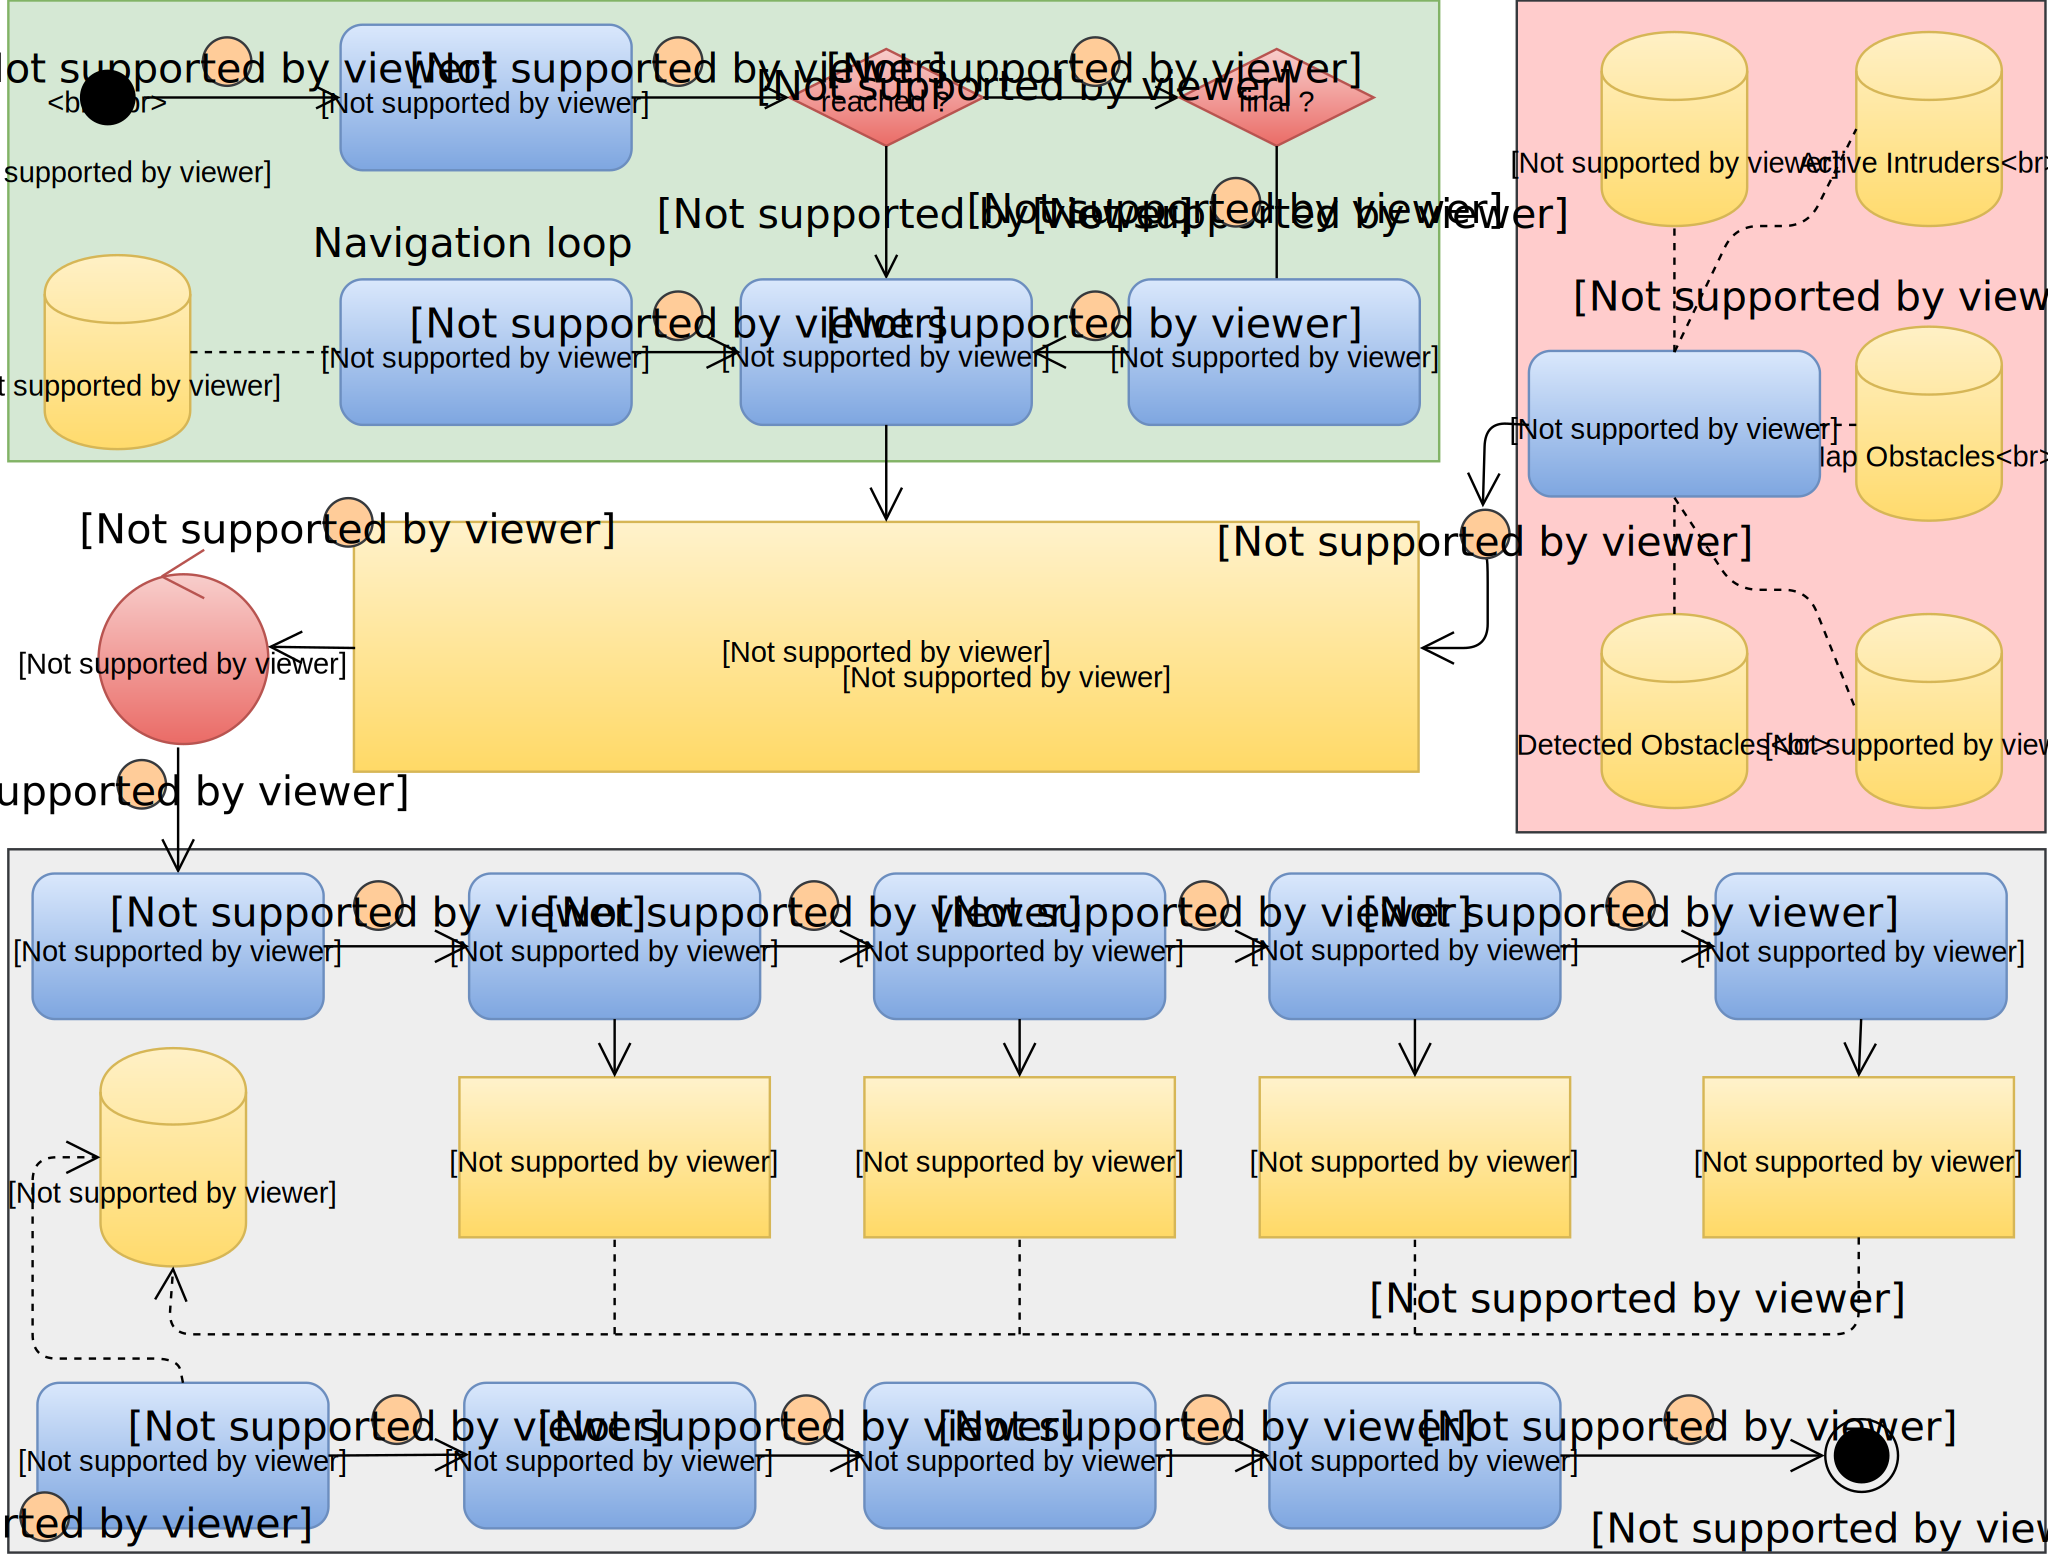
\includegraphics[width=\linewidth]{\FIGDIR/TE026AvoidanceAlgorithmMainLoopRun}
    \caption{Mission control run activity diagram.}
    \label{fig:missionControlRunActivityDiagram}
\end{figure}

\noindent The main changes to \emph{Navigation architecture} are given in \emph{Mission Control Run} activity diagram (fig. \ref{fig:missionControlRunActivityDiagram}):

\begin{enumerate}
    \item \emph{Situation Assessment} - added event-based mode switching control. 
   
    \item \emph{Avoidance Run} - added hierarchical evaluation for \emph{Avoidance Path} selection; This is responsible for prioritizing threat avoidance according to a type. 
\end{enumerate}

\noindent The \emph{Operation Mode} is introduced, based on \emph{Situation assessment} and \emph{Triggering Events} one of the following modes are selected in \emph{Avoidance Run}:

\begin{enumerate}
    \item \emph{Navigation Mode} - the \emph{UAS} is navigating through \emph{Airspace} following \emph{cost-effective patterns} and obeying \emph{Airspace Authority} (UTM). The \emph{Navigation Grid} is an instance of \emph{Avoidance Grid} (sec. \ref{s:AvoidanceGrid}) with initialized \emph{Navigation Reach Set} (ex. \emph{Turn-Minimizing Reach Set Approximation} (sec. \ref{s:harmonicReachSet})).
    
    \item \emph{Emergency Avoidance Mode} - the \emph{UAS} is \emph{threatened} by obstacle, intruder, hard constraint or \emph{soft constraint}, the \emph{UAS} is navigating through \emph{Airspace} following \emph{safe avoidance patterns} and \emph{minimizing the impact} of possible damages. The \emph{Avoidance Grid} is a term used for \emph{Emergency Avoidance Mode}. The \emph{Avoidance Reach Set Approximation} is initialized in \emph{Avoidance Grid} (ex. \emph{Coverage-Maximizing Reach Set Approximation} (sec. \ref{s:chaoticReachSet}))
\end{enumerate}

\begin{note}
    Depending on \emph{Operation Mode} the pair of \emph{Avoidance Grid} and \emph{Reach Set} is selected in \emph{Avoidance Run} part.
    
    
    The \emph{Navigation Grid} and \emph{Avoidance Grid} share the space portioning pattern; therefore the \emph{Data Fusion} (sec. \ref{s:sensorFusion}) needs to be evaluated only once for both grids. 
\end{note}



\paragraph{Decision Time Frame ($[t_i,t_{i+1}[$):} The \emph{Mission Control Run} is executed for \emph{Decision Time Frame} bounded to the \emph{period} of the \emph{UAS executed movement} (fig. \ref{fig:AvoidanceFrameworkConceptNew}).

The \emph{UAS System} (sec. \ref{s:UASNonlinearModel}) controlled by \emph{Movement Automaton Implementation} (sec. \ref{s:movementAutomatonDefinition}) \emph{Planned Movements} can be changed at any time. The real impact on control is shown after the \emph{actual movement} is executed. 

\begin{note}
    For our \emph{Movement Automaton Implementation} movements, the average \emph{movement duration} is \emph{1/velocity second} (tab. \ref{tab:movements1}, \ref{tab:movements2}).
\end{note}

The \emph{Decisions} are made based on \emph{system} state in \emph{current} time-frame started at $t_i$ for the \emph{next} time frame starting at $t_{i+1}$.

\begin{note}
    Because the \emph{Decision Delay} is crucial in \emph{Avoidance System}, it is beneficial to have \emph{short time movements}. On the other hands, the \emph{length and duration  of movements} are impacting \emph{Reach Set Complexity}. The proper construction of movement automaton is greatly impacting overall \emph{approach performance}.
\end{note}

\paragraph{Initialization:} The \emph{UAS} is going to solve a problem for \emph{Rules of the Air} (eq. \ref{eq:rulesOfTheAir}). Using control scheme (fig. \ref{fig:AvoidanceFrameworkConceptNew}) with given \emph{Sensors}:

\begin{equation}
    Sensors = \{LiDAR,ADS-B\}
\end{equation}

\noindent The sensors obstacle assessment into avoidance grid is outlined for static obstacles in (sec. \ref{s:staticObstacles}) and for moving obstacles in (sec. \ref{s:intruders}.)

\noindent The \emph{Data Fusion Procedure} is given as follow:
\begin{equation}
    DataFusion = \{Rating Based Data Fusion \quad (sec. \ref{s:sensorFusion})\}
\end{equation}

Then the \emph{UAS system} (sec. \ref{s:UASNonlinearModel}) with \emph{Movement Automaton Implementation} (sec. \ref{s:movementAutomatonDefinition}) with empty movement buffer:

\begin{equation}
    Movement Buffer = \{\}
\end{equation}

\noindent The \emph{Avoidance Grids} for both \emph{Operation Modes} are created with \emph{identical space segmentation}. The \emph{Reach Set Approximations} are loaded based on initial \emph{UAS State} at decision time $0$. The \emph{Reach Set Approximation} is always selected based on \emph{UAS System State}. The initial \emph{Operation Mode} is set up as \emph{Navigation}. The initialization is summarized like follow:

\begin{equation}
    \begin{aligned}
    Avoidance Grid(0) &= \{UAS.position(0),AvoidanceReachSet(UAS.ReachSet)\}\\
    Navigation Grid (0) &= \{UAS.position(0), NavigationReachSet(UAS.ReachSet)\}\\
    Operation Mode &= Navigation
    \end{aligned}
\end{equation}

The \emph{Mission} is set up as a set of \emph{ordered waypoints}. The \emph{initial goal waypoint} is \emph{first waypoint}. The initialization is summarized like follow:

\begin{equation}
    \begin{aligned}
    Mission &= \{Waypoint_1 \dots  Waypoint_n\}\\
    Goal Waypoint &= Mission.waypoint_1\\
    Last Waypoint &= Mission.waypoint_n\\
    \end{aligned}
\end{equation}

The \emph{actual threats} are set as empty sets for \emph{decision time} $t_i=0$:
\begin{equation}
    \begin{aligned}
    obstacles &= \{\}, intruders = \{\}, hard Constraints = \{\}, soft Constraints = \{\}\\
    \end{aligned}
\end{equation}



\paragraph{Navigation Loop (1\textsuperscript{st}-3\textsuperscript{rd} step):} The purpose of \emph{Navigation Loop} is to select proper \emph{Goal Waypoint} from \emph{Mission} (sec. \ref{s:mission}). If \emph{last waypoint} have been reached the \emph{Landing Procedure} will be initiated and \emph{Mission Control Run} Ends.

First, start with the definition of \emph{waypoint reach condition} (def. \ref{def:waypointReachCondition}) and \emph{Unreachable waypoint} (def. \ref{def:unreachable Waypoint}).

\begin{definition}{Waypoint Reach Condition}\label{def:waypointReachCondition} for \emph{current} decision time $t_i$ for \emph{UAS} position and current \emph{Goal Waypoint} is satisfied only if:

\begin{multline}\label{eq:waypointReachCondition}
    distance(UAS.position(t_i),GoalWaypoint(t_i)) \\\le \\2 \times \max \left\{length(movement):\forall movement\in MovementSet\right\}
\end{multline}

    \begin{note}
        The movements in our solution have a \emph{uniform length} of \emph{1 m} (tab. \ref{tab:movements1}, \ref{tab:movements2}), therefore the waypoint reach condition is satisfied when the \emph{distance to goal waypoint} is lesser than 2 m. The maximal movement length has an impact on \emph{navigation/avoidance} precision.
    \end{note}
\end{definition}

\begin{definition}{Unreachable Waypoint}\label{def:unreachable Waypoint}. The \emph{Goal Waypoint} evaluates as unreachable in decision time $t_i$ when \emph{Avoidance Grid Run} (alg. \ref{alg:FindBestPathAvoidanceGrid}) cannot find the \emph{navigation/avoidance path} leading to it.

\noindent Formally: The \emph{Avoidance/Navigation Grid} has range defined as \emph{final layer distance}. When the \emph{Goal Waypoint} is in  \emph{range} of \emph{Grid}:

\begin{equation}
    Grid(t_i).range \ge distance(UAS.position(t_i),GoalWaypoint(t_i))
\end{equation}

\noindent and following condition is satisfied:

\begin{multline}\label{eq:unreachableWaypoint}
    \forall cell_{i,j,k}\in Grid(t_i) \not\exists cell_{i,j,k}. Reachable == true \wedge\dots  \\\dots\wedge distance(cell_{i,j,k}, Goal Waypoint(t_i)) \le\dots \\ \dots\le 2 \times \max \left\{length(movement):\forall movement\in MovementSet\right\}
\end{multline}

\noindent The \emph{Goal Waypoint} is unreachable.

\end{definition}

Then the \emph{Navigation Loop} is invoked  every \emph{decision time} $t_i$, \emph{Mission Control Run} (fig. \ref{fig:missionControlRunActivityDiagram}), it is described as a sequence of the following steps:

\begin{itemize}
    \item[\textbf{1\textsuperscript{st}}] \textbf{Check Waypoint Reach Condition} - the \emph{UAS position} for given a \emph{time frame} $t_i$ is checked under condition (eq. \ref{eq:waypointReachCondition}).  If the condition is met continue with 2\textsuperscript{nd} step otherwise continue with 3\textsuperscript{rd} step.

    \item[\textbf{2\textsuperscript{nd}}] \textbf{Set Next Waypoint} - until the following condition is met:
    \begin{equation*}
        Goal Waypoint == Last Waypoint    
    \end{equation*}
    Set next goal waypoint like follow:
    \begin{equation*}
        Goal Waypoint = Mission.get Next Waypoint()
    \end{equation*}
    Otherwise, enforce \emph{Landing sequence} (Out of Scope).
        
    \item[\textbf{3\textsuperscript{rd}}] \textbf{Trajectory Prediction} - the \emph{Movement Buffer} is loaded with planned movements from \emph{Movement Automaton}. The \emph{future trajectory} is predicted according to (eq. \ref{eq:ourTrajectoryImplementation}):
    \begin{multline*}
        Predicted Trajectory = \\Trajectory(state=UAS.state(t_i),buffer=future Movements)
    \end{multline*}
\end{itemize}

\noindent The \emph{Predicted Trajectory} is used in 5\textsuperscript{th} step \emph{Situation Assessment}.

\paragraph{Data Fusion (4\textsuperscript{th} step)} The \emph{Data Fusion} (sec. \ref{s:sensorFusion}) in this context is \emph{Threat Sets} preparation for \emph{Avoidance Run}. It depends on the values of \emph{Boolean values} defined in (tab. \ref{tab:defuzificationRatings}) for \emph{threat} classification.

\begin{note}
    Avoidance Grid`s Data fusion (sec. \ref{s:sensorFusion}) is run in the  7\textsuperscript{th}- 10\textsuperscript{th} step (fig. \ref{fig:missionControlRunActivityDiagram}). 
\end{note}

The \emph{static obstacles} source is from \emph{LiDAR} scan received at least at the  beginning of current \emph{decision frame} $t_i$:

\begin{equation*}
        obstacles=LiDAR.scan(UAS.position(t_i))
\end{equation*}

The \emph{intruder`s} source are valid \emph{active intruders notifications} received from ADS-B In positioned to \emph{future expected positions} at \emph{decision time} $t_{i+1}$:

\begin{equation*}
        intruders=ADS-B.get Active Intruders(t_{i+1})
\end{equation*}

\begin{note}
    The \emph{Intruders} needs to be predicted for the next decision time-frame starting at time $t_{i+1}$ Due to their mobility.
\end{note}

\noindent The \emph{hard/soft constraints} are obtained from \emph{Information Sources} and the area of next decision time $t_{i+1}$ \emph{Avoidance Frame} is used as space parameter in the search. The sets of hard and soft constraints are obtained in the following manner:

\begin{equation*}
    hard Constraints= Information Sources.fuse(Avoidance Grid(t_{i+1}))
\end{equation*}

\begin{equation*}        
        soft Constraints=Information Sources.fuse(Avoidance Grid(t_{i+1}))
\end{equation*}

\noindent The results of \emph{Data Fusion} threats set preparation are used in the next step.


\paragraph{Invoke Navigation/Avoidance based on Situation Assessment (5\textsuperscript{th}-6\textsuperscript{th} step):} The \emph{deciding events} depending on \emph{Trajectory Prediction} ($3^{rd}$ step) and \emph{Data Fusion} ($4^{th}$ step) (fig. \ref{fig:missionControlRunActivityDiagram}) are the following:

\begin{enumerate}
    \item \emph{General Events} are \emph{triggered} regardless \emph{Operation Mode}. They are considered after \emph{specific mode events} are handled and \emph{Navigation/Avoidance Grid} is selected:
    \begin{enumerate}[a.]
        \item \emph{Empty Movement Buffer} ($Movement Buffer = \varnothing$) - if there is no movement in \emph{Movement buffer} to be executed (from 3\textsuperscript{rd} step: Load Trajectory), the \emph{Avoidance Run} is enforced to run with \emph{Navigation/Avoidance Reach Set Approximation} to generate the new path.
        
        \item \emph{Waypoint Reached} (2\textsuperscript{nd} step) - the \emph{Navigation Loop} run is forced to set goal \emph{Goal Waypoint}. If the \emph{last waypoint} from \emph{Mission} (sec. \ref{s:mission}) the \emph{Landing Procedure} is enforced.
        
        \item \emph{Waypoint Unreachable} - this type of event is very situations based. The \emph{Waypoint Reachability} (assumption. \ref{ass:reachableWaypoints}) has not been relaxed; therefore this event is not properly handled in approach. The \emph{implementation} considers \emph{selecting next waypoint in the mission} as a goal waypoint of the \emph{first waypoint} if \emph{unreached/unreachable waypoints} are exhausted. 
    \end{enumerate}
    
    \item \emph{Navigation Mode Events} are triggered if \emph{Operation Mode} is set as \emph{Navigation}:
    \begin{enumerate}[a.]
        \item \emph{Empty Navigation Grid} ($|threats| = 0$) - if \emph{movement buffer} contains at least one \emph{movement}, the \emph{Avoidance Run} is omitted. The \emph{Operation Mode} stays in \emph{Navigation Mode}.
        
        \item \emph{Collision Case Resolution} ($|ActiveCollisionCases| > 0$) - there is new/active \emph{Collision Case} (sec. \ref{sec:collisionCase}), the \emph{Navigation Reach Set Approximation} trajectories will be constrained according to  active \emph{Collision Case(s)} requirements. If there exists at least one \emph{Reachable} avoidance path, the \emph{Operation Mode} will remain \emph{Navigation}. If there is no  \emph{Reachable} avoidance path, the \emph{Operation Mode} switches to \emph{Emergency Avoidance}.
        
        \item \emph{Static Obstacle Detection} ($LiDAR.Hits > threshold$) - if \emph{static obstacle set} contains at least one \emph{detected obstacle} (eq. \ref{eq:naiveObstacleRate}) intersecting with \emph{Navigation  grid} the \emph{Operation Mode} will be \emph{switched} to \emph{Emergency Avoidance Mode}.
        
        \item \emph{Intruder Detection} ($intruders> 0$) - if \emph{active intruders set} contains at least one \emph{intruder} which expected impact area (intersection models (app. \ref{app:IntruderProbabilisticModels})) \emph{Navigation  grid} the \emph{Operation Mode} will be \emph{switched} to \emph{Emergency Avoidance Mode}.
        
        \item \emph{Hard or Soft Constraint Occurrence} ($|hard Constraints|$ $>$ $0$ $\vee$ $|soft Constraints|$ $>$ $0$) - if \emph{hard/soft constraint set} contains at least one \emph{constraints} which intersects (static constraints (sec. \ref{s:virtualConstraints}), moving constraints (def. \ref{def:movingConstraint})) \emph{Navigation  grid} the \emph{Operation Mode} will be \emph{switched} to \emph{Emergency Avoidance Mode}.
    \end{enumerate}
    
    \item \emph{Emergency Avoidance Events} are triggered if \emph{Operation Mode} is set as \emph{Emergency Avoidance}:
    \begin{enumerate}[a.]
        \item \emph{Empty Avoidance Grid} ($|threats| = 0$) - if there is no \emph{detectable} threat, the remainder of \emph{avoidance path} is removed from \emph{Movement Buffer}. The \emph{Operation Mode} is switched to \emph{Navigation}, and new \emph{navigation path} is selected. 
    \end{enumerate}
\end{enumerate}



\begin{itemize}
    \item[\textbf{5\textsuperscript{th}}] \textbf{Situation Assessment} - if there is any flag raised by \emph{Event Triggers}, there is an \emph{avoidance situation}.
    
    The \emph{Event Triggers} describe complex \emph{Operation Mode} switching. The simplified principle is the following: \emph{If UAS is in Emergency Avoidance Mode Always Invoke Avoidance Run. If UAS is in Navigation Mode Invoke Only if Necessary}.
    
    If there was event trigger continue with 7\textsuperscript{th} step, otherwise, wait for \emph{next decision time} $t_{i+1}$, execute movement and continue with 1\textsuperscript{st} step.
    
    \item[\textbf{6\textsuperscript{th}}] \textbf{Invoke Navigation/Avoidance} depending on the \emph{Operation Mode} the \emph{Reach Set/Grid} pair is selected. The future $state(t_{i+1})$ in next decision frame $t_{i+1}$ is necessary for Grid/Reach Set initialization. The \emph{next decision frame initial state} is obtained by \emph{prediction}:
    
    \begin{equation*}
        state(t_{i+1}) =  Trajectory(state(t_i),current Movement)
    \end{equation*}
    
    The \emph{Reach Set Approximation} is loaded based on \emph{mode} and $state(t_{i+1})$. The \emph{Grid} is initialized as $Free(t_{i+1})$ (eq. \ref{eq:freeDataFusion}) for all cells.
\end{itemize}



\paragraph{Avoidance Run (7\textsuperscript{th}-15\textsuperscript{th} step):} The \emph{Avoidance Run} goal is to obtain \emph{Path} represented as \emph{Trajectory}(state($t_{+1}$,MovementBuffer)) (eq. \ref{eq:ourTrajectoryImplementation}) from \emph{Navigation/Avoidance Grid} and associated \emph{Navigation/Avoidance Reach Set Approximation}.

If the \emph{Operation Mode} is set as \emph{Navigation Mode}, the algorithm continues with the 11\textsuperscript{th} step. Otherwise, the \emph{Avoidance Grid Space Assessment} is run multiple times to obtain $Reachable(t_{i+1})$ (eq. \ref{eq:ReachableDataFusion}). The \emph{Threat Data} obtained from the 4\textsuperscript{th} step are used. 

\begin{itemize}
    
    \item[\textbf{7\textsuperscript{th}}] \textbf{Apply Obstacles} - The \emph{Space assessment} (tab. \ref{tab:defuzificationRatings}) for \emph{Avoidance Grid} is calculated  with following threat modification:
    
    \begin{equation*}
        intruders = \varnothing, soft Constraints = \varnothing, hard Constraints = \varnothing
    \end{equation*}
    
    The \emph{Find Best Path} (alg. \ref{alg:FindBestPathAvoidanceGrid}) is applied, the resulting \emph{avoidance path} is labeled as \emph{Obstacle Avoidance Path}.
  
    \item[\textbf{8\textsuperscript{th}}] \textbf{Apply Intruders} - The \emph{Space assessment} (tab. \ref{tab:defuzificationRatings}) for \emph{Avoidance Grid} is calculated  with following threat modification:
    
    \begin{equation*}
        soft Constraints = \varnothing, hard Constraints = \varnothing
    \end{equation*}
    
    The \emph{Find Best Path} (alg. \ref{alg:FindBestPathAvoidanceGrid}) is applied, the resulting \emph{avoidance path} is labeled as \emph{Intruders Avoidance Path}.
    
    \item[\textbf{9\textsuperscript{th}}] \textbf{Apply Hard Constraints} - The \emph{Space assessment} (tab. \ref{tab:defuzificationRatings}) for \emph{Avoidance Grid} is calculated  with following threat modification:
    
    \begin{equation*}
        hard Constraints = \varnothing
    \end{equation*}
    
    The \emph{Find Best Path} (alg. \ref{alg:FindBestPathAvoidanceGrid}) is applied, the resulting \emph{avoidance path} is labeled as \emph{Hard Constraint Avoidance Path}.
    
    \item[\textbf{10\textsuperscript{th}}] \textbf{Apply Soft Constraints} - The \emph{Space assessment} (tab. \ref{tab:defuzificationRatings}) for \emph{Avoidance Grid} is calculated  without any modification.
    
    The \emph{Find Best Path} (alg. \ref{alg:FindBestPathAvoidanceGrid}) is applied, the resulting \emph{avoidance path} is labeled as \emph{Soft Constraints Avoidance Path}.
    
    \begin{note}
        The 7\textsuperscript{th} to 10\textsuperscript{th} steps are code-optimized for efficient calculation.
    \end{note}
    
    \item[\textbf{11\textsuperscript{th}}] \textbf{Select Path} -  based on \emph{Operation Mode} the \emph{Navigation/Avoidance Path} is selected.
    
    The \emph{Navigation Path} for \emph{Navigation Mode} is selected by a standard \emph{Find Best Path} (alg. \ref{alg:FindBestPathAvoidanceGrid}) procedure. The \emph{Navigation Reach Set Approximation} can be constrained by \emph{Rule Engine} (fig. \ref{fig:RuleEngineInstanceLevels}).
    
    The \emph{Avoidance Path} for \emph{Emergency Avoidance Mode} is selected from \emph{Collected Avoidance Paths} with the following priority:
    \begin{itemize}
        \item[1.] \emph{Soft Constraints Avoidance Path} - if exists continue with 12\textsuperscript{th} step, if does not exist try to select:
        
        \item[2.] \emph{Hard Constraints Avoidance Path} - if exists continue with 12\textsuperscript{th} step, if does not exist try to select:
        
        \item[3.] \emph{Intruders Avoidance Path} - if exists continue with 12\textsuperscript{th} step, if does not exist try to select:
        
        \item[4.] \emph{Obstacle Avoidance Path} - continue with the 12\textsuperscript{th} step.
    \end{itemize}
    \begin{note}
        The \emph{Waypoint Reachability} (assumption \ref{ass:reachableWaypoints}) is weakened to the point that it is necessary for the waypoint to be \emph{Reachable} only in static obstacle environment. The \emph{Constrained} and \emph{Occupied} spaces are shrunk in the following matter to increase UAS survival chances. There are following relaxations with their conditions:
        \begin{itemize}
            \item[1.] \emph{Soft Constraint Relaxation} - they are breakable by default.  This kind of situation is allowed to happen under any circumstances. 
            
            \item[2.] \emph{Hard Constraints Relaxation} - they can be broken in case of emergency (airspace constraints) or UAS robust build (Weather Constraints). This kind of situation is allowed under very specific conditions depending on \emph{broken constraint} severity.
            
            \item[3.] \emph{Intruder Occupied Space Relaxation} - this can be broken if and only if there is guarantee the Intruder dynamic and navigation algorithm allows to avoid \emph{Collision} with UAS. This relaxation should be used as \emph{the last resort}.
        \end{itemize}
    \end{note}
    
    \item[\textbf{12\textsuperscript{th}}] \textbf{Load Movements} - the \emph{Movement Buffer} is flushed for \emph{future decision times} $t_{i+1}, \dots, t_{i+k}$. The \emph{Navigation/Avoidance Path} movements are pushed into \emph{Movement Buffer} instead. The \emph{executed movement} for \emph{decision time} $t_i$ remains (because movement is executed at this time point).
    
    \item[\textbf{13\textsuperscript{th}}] \textbf{Set Next Decision} - the \emph{next decision point} is set depending on circumstances:
    \begin{itemize}
        \item[1.] Navigation Mode (no active collision cases) - \emph{Decision Point} is set as the point before \emph{UAS} enters into \emph{Crash Zone} (fig. \ref{fig:gridZonesMissionControl}) in \emph{Navigation Grid}.
        
        \item[2.] \emph{Navigation Mode (at least one active collision case)} - \emph{Decision Point} is set after \emph{next movement execution}. Current decision point $UAS.Position(t_i)$, next decision point $UAS.Position(t_{i+1})$.
        
        \item[3.] \emph{Emergency Avoidance Mode (any circumstances)} - \emph{Decision Point} is set after the \emph{next movement execution}. Current decision point $UAS.Position(t_i)$, next decision point $UAS.Position(t_{i+1})$.
    \end{itemize}
    
    \item[\textbf{14\textsuperscript{th}}] \textbf{Execute Movement} - the \emph{First Movement} from \emph{Movement Buffer} is loaded to be executed in decision time frame $[t_{i+1}, t_{i+2}[$. 
    
    \item[\textbf{15\textsuperscript{th}}] \textbf{Finish Avoidance Run} - if the \emph{UAS} is flying, continue with 1\textsuperscript{st} step. 
\end{itemize}

\newpage
\paragraph{Decision Frame:} The \emph{mission control run} (fig. \ref{fig:missionControlRunActivityDiagram}) describes the overall process in \emph{sequence}. The \emph{orchestration overview} is given in (fig. \ref{fig:misisonControlRunOrchestrationDiagram}).

The key idea is to explain what happens in one \emph{decision frame}. The \emph{mission control run} is implemented as multi-thread application which sends the signals between threads. Each thread is the semi-independent process with forced synchronization on \emph{decision frame switch}.

\begin{figure}[H]
    \centering
    \includegraphics[width=\linewidth]{\FIGDIR/TE064DecisonFrameExplained}
    \caption{Mission control orchestration diagram.}
    \label{fig:misisonControlRunOrchestrationDiagram}
\end{figure}

\noindent The notable threads and their roles \& responsibilities are summarized like follow:
\begin{itemize}
    \item[1.] \emph{Sensor Fusion} - responsible for processing real-time sensor array (sec. \ref{s:SensorFusionDefinition}). The output is a partial known world assessment (sec. \ref{s:KnownWorld}). \emph{Obstacle detection} and \emph{intruder detection} events can be risen by this thread. 
    
    \item[2.] \emph{Data Fusion} - responsible for enhancing data from \emph{sensor fusion} by mixing data originating from \emph{information sources} (sec. \ref{s:dataFusionDefinition}). The information sources used in this work contains constraints originating from \emph{geo-fencing}, \emph{weather}, \emph{airspace restrictions}. This thread is delayed by \emph{sensor fusion}. A \emph{data fusion procedure} strongly depends on the \emph{operational space context} (controlled/non-controlled airspace). The output of \emph{data fusion} is full \emph{known world assessment} (sec. \ref{s:KnownWorld}, \ref{s:sensorFusion}). The \emph{UTM-related} and \emph{constraint related} events can arise from \emph{data fusion}.
    
    \item[3.] \emph{Event Buffer} -  special data structure to store, raise, handle, prioritize events raised by other threads. 
    
    The \emph{implemented events} are listed in the  5\textsuperscript{th}-6\textsuperscript{th} step of \emph{mission control run}. The events can be categorized like follow:
    \begin{itemize}
        \item[a.] \emph{Planned events} - raised in previous decision frames to be executed in actual or future \emph{decision frame}. 
        
        \item[b.] \emph{Intermediate events} - raised in \emph{actual decision frame} by other threads to be solved intermediate. 
    \end{itemize}
    
    The event buffer thread executes following event-related activities:
    \begin{itemize}
        \item[a.] \emph{Storing} - the \emph{events} are stored in the \emph{event log}. The trace is useful for process and rules fine-tuning. 
        
        \item[b.] \emph{Raising} - the combination of events (multiple avoidance events) (example sec. \ref{s:testRuleMixed}) can trigger additional avoidance behavior in the form of combined-event.
        
        \item[c.] \emph{Handling} - the events are handled by invoking the \emph{situation assessment} or by rule engine invocation (sec. \ref{s:RuleEngineArchitecture}).
        
        \item[d.] \emph{Prioritizing} - the multiple events can rise during one \emph{decision frame}. Some events cannot be merged and need to have proper prioritization before handling, like the \emph{obstacle detection} events before \emph{intruder detection event}.
    \end{itemize}
    
    \item[4.] \emph{Situation Assessment} - invoked by \emph{event buffer} to assess the situation, responsible for proper \emph{avoidance run} (sec. \ref{s:aviudabceGridRun}) dataset preparation and invocation. The main responsibility is to check \emph{planned trajectory feasibility} stored in \emph{movement buffer} as \emph{planned movements}.
    
    \item[5.] \emph{Avoidance Run} - invoked by \emph{necessity to plan trajectory} originating from \emph{event buffer} or \emph{situation assessment} threads. The avoidance run produces one or multiple \emph{avoidance/navigation} feasible trajectories according to  the 7\textsuperscript{th}-11\textsuperscript{th} step of \emph{mission control run}.
    
    \item[6.] \emph{Movement Buffer} - represents \emph{movement automaton implementation} (sec. \ref{s:movementAutomatonDefinition}). The movement automaton consumes \emph{movement automaton buffer} each decision frame contains exactly one \emph{movement}. The movements can be viewed as:
    \begin{itemize}
        \item[a.] \emph{Past movements} - already executed movements in \emph{past decision frames}.
        
        \item[b.] \emph{Executed movement} - actually executed movement in the current decision frame, this movement cannot be changed.
        
        \item[c.] \emph{Future movements} - future planned movements to be executed after \emph{current decision frame} expires. These movements outline planned trajectory (predictor mode sec. \ref{s:referenceTrajectoryGenerator}).
    \end{itemize}
    
    \item[7.] \emph{Feasible Trajectory} - consists of \emph{future planned movements} taking place directly after the \emph{correct decision frame}. If its necessary, the planned trajectory in movement buffer is no longer feasible, the planned movements will throw away and replaced by \emph{trajectory movements}. 
\end{itemize}

\newpage
\noindent The \emph{roles \& responsibilities} of each thread have been explained to outline their orchestration and roles in \emph{mission control run} (fig. \ref{fig:missionControlRunActivityDiagram}). The numbered steps in (fig. \ref{fig:misisonControlRunOrchestrationDiagram}) shows the threads orchestration in the following manner:

\begin{itemize}
    \item[1.] \emph{Sensor \& Data fusion data set preparation/collection} - the sensor readings are collected through multiple past and over current \emph{decision frame}. Each sensor reading is filtered and processed according to best practices. 
    
    The raw information from various data sources is loaded for relevant space clusters. The relevant space clusters are determined based on \emph{UAS expected position}. 
    
    \item[2.] \emph{Sensor fusion} - the readings from sensors are preprocessed according to (sec. \ref{s:staticObstacles}, \ref{s:intruders}).
    
    \item[3.] \emph{Data fusion} - the information sources are preprocessed according to (sec. \ref{s:staticObstacles}, \ref{s:intruders}).
    
    \item[4.] \emph{Event evaluation process} - the events are evaluated, if there is any triggering event (5\textsuperscript{th}-6\textsuperscript{th} mission control run steps) the situation evaluation process is called.
    
    \item[5.] \emph{Situation evaluation process} - the situation is evaluated according to 5\textsuperscript{th}-6\textsuperscript{th} mission control run steps.
    
    \item[6.] \emph{Feasible trajectory selection process} - from collected \emph{navigation/avoidance trajectories} (7\textsuperscript{th}-10\textsuperscript{th} mission control run steps). If there are more feasible trajectories (increasing threat) the one compliant with most of the threats is selected.
    
    \item[7.] \emph{Movement execution} - the movement for the \emph{current decision frame} is being executed.
    
    \item[8.] \emph{Movement buffer swap} - if there is a new \emph{feasible trajectory} the future movements for next decision frames are flushed away. The movement buffer is then filled with \emph{feasible trajectory movements}.
    \begin{note}
        This step impacts the duration of future \emph{decision frames}.
    \end{note}
\end{itemize}

    	\subsection{(R) Safety Margin Calculation}\label{s:safetyMarginCalculation}
\paragraph{Safety Margin Determination:} To determine \emph{safety Margin} the \emph{Rule of Thumb} is used:

\begin{equation}
    maximal Body Radius \le safety Margin \le 2 \times turning Radius
\end{equation}

\noindent The \emph{lower boundary} is given by \emph{UAS} construction. because the \emph{UAS} body is considered as \emph{unit ball} with radius given as \emph{maximal body radius}. 

The \emph{upper boundary} is optional, The \emph{double of \emph{turning radius}} is used by the \emph{conservative approach} \cite{borenstein1991vector}.


\paragraph{Safety Margin Bloating:}  The \emph{discretization} of \emph{Reach Set}, \emph{Operation Space} and \emph{Decisions} imposes standard \emph{mixed integer} problem in terms of \emph{safety}. This section covers \emph{non-exhaustive} list of possible \emph{Safety Margin Bloats} in our approach.

\paragraph{Own Position Uncertainty Bloat:} The \emph{sensor fusion} is precise, but not \emph{exact} in own UAS position determination. The maximal usual disparity needs to be accounted into \emph{Safety Margin}.

\paragraph{Intruder Position Uncertainty Bloat:} The \emph{sensor fusion} of Intruder is precise, but not \emph{exact} in own UAS position determination. The maximal usual disparity needs to be accounted into \emph{Safety Margin}.

\paragraph{Weather bloat:} The \emph{Weather} impact type may result to increased \emph{safety margin}. Example: UAS is not humidity resistant, the clouds will be avoided from greater distance.

\paragraph{Airspace bloat:} The \emph{Airspace} depending on cluster or \emph{country} may require greater separation distances, depending on circumstances. The example can be UAS directive to keep minimal separation from obstacles. The \emph{Safety Margin} is usually overridden by UTM directive value.

\paragraph{UTM Synchronization Bloat:} \emph{Both UAS} decision times were \emph{synchronized}. The \emph{intruder} can be offset for \emph{full decision frame}. This is not an assumption, but it shows critical performance. Usually safety margin is bloated for (worst case offset):
\begin{equation}\label{safetyMarginBloat}
    safetyMarginBloat = \left( \begin{aligned}
    &intruderVelocity \times\dots \\ &intruderDecisionFrame \end{aligned}\right)[m,ms^{-1},s]
\end{equation}
    
    %06-08 UTM implementation
		\cleardoublepage
\section{\secState{R}UAS Traffic Management}\label{sec:UASTrafficManagement}

\noindent The \emph{Traffic Management} for UAS is based on existing Air Traffic Management System for manned aviation \cite{icao4444}. The controlled airspace segments are \emph{static} and have one \emph{authority for one zone} principle. The dynamic zones have been proposed in \cite{gerdes2016dynamic}. However, it will be omitted for \emph{simplification purpose}. The necessity for \emph{UAS integration} into \emph{National Airspace} has been outlined in \cite{spriesterbach2013unmanned}.

The latest \emph{Airbus blueprint} \cite{airbusUTM2018blueprint} outlines some functionality. The main purpose of this section is to show \emph{Reach Set based Approach} capability to follow \emph{Usual Air Traffic Management} commands.

The \emph{section} is organized to introduce:
\begin{enumerate}
    \item \emph{UTM Architecture} (sec. \ref{sec:utmArchitecture}) - centralized ATM-like authority over airspace cluster.
    
    \item \emph{Handling Standard Collision Situations} - head-on approach (sec. \ref{sec:handlingHeadOnApproach}), converging situation (sec. \ref{sec:handlingConvergingManuever}), overtake (sec. \ref{sec:handlingOvertakeManuever}).
    
    \item \emph{Position Notification} (sec. \ref{sec:positionNotification}) - position notification design.
    
    \item \emph{Collision Case} (sec. \ref{sec:collisionCase}) - calculation and handling of \emph{collision situations}.
    
\end{enumerate}

\noindent The additional material can be found in:
\begin{enumerate}
	\item \emph{Cooperative Conflict Resolution} (app. \ref{sec:cooperativeConflictResolution}) - the model used for conflict resolution in \emph{controlled airspace}.
    
    \item \emph{Non-Cooperative Conflict Resolution} (app. \ref{sec:nonCooperativeConflictResolution})  - the model used for conflict resolution in \emph{non-controlled} airspace and \emph{emergency avoidance}.
    
    \item \emph{Weather Case} (app. \ref{sec:weatherCase}) - definition and handling of \emph{weather hazards}.
\end{enumerate}
		\subsection{\secState{R}Architecture}\label{sec:utmArchitecture}
\paragraph{UTM Concept} is based on \emph{asynchronous event-based control} \cite{zimmer2011rule}. \emph{Event} in \emph{controlled airspace} is handled in form of \emph{cases} \cite{prevot2016uas}. There are following \emph{event sources}:

\begin{enumerate}
    \item \emph{Weather Information Service} (from \cite{zimmer2014selective}) - used to create \emph{weather case} (tab. \ref{tab:weatherConstraint}).
    
    \item \emph{Position Notification from UAS systems} (tab. \ref{tab:positionNotification}) - used to create \emph{collision cases} (new functionality) (tab. \ref{tab:collisionCase}).
\end{enumerate}


\paragraph{Decision Frame} (eq. \ref{eq:decisionFrameDefinition}). The \emph{UTM} is operating in discrete decision frames which are starting on current \emph{decision time} and ending at  next \emph{decision  time}:

\begin{equation}\label{eq:decisionFrameDefinition}
    decision Frame_i = [decision Time_i, decision Time_{i+1}[,\quad i \in {1,\dots,k}, k \in \N^+
\end{equation}

\paragraph{Event-based Airspace Control} is collecting  events in  previous $decisionFrame_{i-1}$ and issuing commands in current $decisionFrame_i$.There are following phases during the \emph{UTM frame} cycle:
\begin{enumerate}
    \item \emph{Planning} - the detection phase, when the hazardous situations are assessed.
    
    \item \emph{Fulfillment} - the monitoring phase, when the state of affairs for directives and mandates is full filled by controlled UAS systems. 
    
    \item \emph{Acknowledgement} - the closing phase, when UTM assess and acknowledges the performance of controlled UAS systems.
\end{enumerate}


\begin{figure}[H]
    \centering
    \includegraphics[width=0.7\linewidth]{\FIGDIR/RE002UTMCommunicationDiagram} 
    \caption{UAS Traffic Management (UTM) architecture overview.}
    \label{fig:UTMArchitectureOverview}
\end{figure}

\paragraph{Architecture} (fig. \ref{fig:UTMArchitectureOverview}).  There are multiple UAS systems equipped with standard \emph{Mission Control} and \emph{Navigation} procedures. 

Depending on the \emph{airspace cluster} decision time frame they are sending \emph{periodical position notifications} (tab. \ref{tab:positionNotification}).

The \emph{UAS Traffic Management} (UTM) collects the event data from \emph{Weather Information Service} and \emph{Position Notifications} calculating respective \emph{cases}. 

If there is an \emph{active collision/weather case} the \emph{UTM} will send \emph{resolutions} to respective airspace attendants. 
		\subsection{(R) Cooperative Conflict Resolution}\label{sec:cooperativeConflictResolution}


\paragraph{Idea:} There is a \emph{final decision maker} (absolute authority) in conflict resolution. This authority is \emph{UTM} or \emph{air traffic attendant} with higher priority. The future \emph{UTM system} is such authority. The approach to mixed conflict resolution is mentioned in \cite{ramasamy2014towards}, based on navigation \cite{ramasamy2013novel}. This is similar to our approach. 

\begin{note}
    \emph{Open Issue:} Decentralized model with UTM as approver of directives is possible, but that is topic for own research.
\end{note}

\paragraph{Goal:} UAS is obligated to follow up committed mission plan with given precision.  There is one to five percent  allowed deviations for ATM mission plans.     Similar rates are achievable according to \cite{ramasamy2014towards}.  This requirement is given by \cite{icao4444} ICAO 4444 document for ATM operations.

\begin{figure}[H]
    \centering
    \includegraphics[width=0.7\linewidth]{\FIGDIR/RE003CooperativeResolution} 
    \caption{Cooperative conflict resolution via UTM authority.}
    \label{fig:CooperativeConflictResolutionUTM}
\end{figure}

\paragraph{Cooperative conflict resolution} (fig. \ref{fig:CooperativeConflictResolutionUTM}) shows functional diagram of one \emph{UTM time-frame} there  are following actors:
\begin{enumerate}
    \item \emph{Unmanned Autonomous System} (UAS) equipped with necessary navigation and communication modules, providing the unique \emph{identification number}.
    
    \item \emph{UAS Traffic Management} (UTM) posing as central authority for given \emph{airspace cluster}.
\end{enumerate}

\noindent The following steps are executed during \emph{Cooperative conflict resolution}:
\begin{enumerate}
    \item $UAS_* \to UTM$ \emph{Send position notification} - each \emph{UAS} is notifying the authority (UTM)
    
    \item $\circlearrowright UTM$ \emph{Calculate collision Cases} - UTM gathers data and predicts possible collisions then it tries to link them and manage the situation.
    
    \item $\circlearrowright UTM$ \emph{Create virtual Roundabout} - active collision cases are aggregated into virtual roundabout. 
    
    \item $UTM \to UAS_*$ \emph{Send directives} - UTM sends commands to UAS systems whom needs to change their planned trajectories. 
    
    \item $UTM \to UAS_*$ \emph{Enforce directives} - UTM is periodically checking constraints imposed in previous \emph{decision frames}.
\end{enumerate}
		\subsection{(R) Non-Cooperative Conflict Resolution}\label{sec:nonCooperativeConflictResolution}

\paragraph{Idea:} There is \emph{main UAS(1)} which is flying in open \emph{non-controlled} airspace. There are other \emph{UAS} operating in its vicinity. It is expected that they are claiming their \emph{planned trajectories}. The \emph{Main UAS(1)} detects the collision with other \emph{UAS}(2-4).

There is no \emph{final decision maker} nor \emph{supervising authority}, all communication participants have similar level of rights. 
\begin{note}
    There is assumption that other airspace users are behaving like intruders, without intent to destroy or harm. The \emph{adversarial behaviour} is not accounted. The response from \emph{intruder} is not mandatory in \emph{non-controlled} airspace.
\end{note}

\paragraph{Goal:} Provide \emph{mutual avoidance mechanism} in \emph{non-controlled} airspace. Considering the equal standpoint of all airspace attendants.

\paragraph{Conflict resolution:} The conflict resolution depends on current mode and \emph{handshake} between airspace attendants. The non-cooperative behaviour have been implemented like follows:

\begin{enumerate}
    \item\emph{Navigation mode} - every \emph{airspace attendant} is calculating own \emph{collision cases} and checking the behaviour of the other (virtual UTM).
    
    \item\emph{Emergency avoidance mode} - is depending on communication mode:
    \begin{enumerate}[a]
        \item\emph{Response mode} - claiming separation methods and using avoidance mechanism (Avoidance grid with intruder model in our case).
        
        \item\emph{Blind mode} - every conflict side picks own strategy respecting given \emph{rules of the air}.
    \end{enumerate}
\end{enumerate}

\begin{note}
    \emph{Intruder Intersection model selection:} UAS based on Event detects possible collision for some reason UTM directive is out of question, then try to claim separation (body volume intruder model (sec. \ref{s:bodyvolumeIntersection})), If separation fails, go full survival mode (uncertain intruder model (sec. \ref{s:bodyvolumeIntersection})).
\end{note}

\paragraph{Special cases in manned aviation:} There are IFALPA reports which can give us overview of \emph{enforced non-cooperative} mode causes in \emph{controlled airspace}:  
\begin{enumerate}
    \item \emph{VFR disabled} - flying in fog or thick clouds can render pilot vision, similar to UAS cameras/LiDAR.
    
    \item \emph{IFR equipment broke} - the sensor malfunction is more likely to happen due the lesser redundancy in UAS systems.
    
    \item \emph{C2C Link disabled} - communication loss is more likely to happen, due the lesser redundancy.
    
    \item \emph{ATM failure} - the ground control module of UTM can also fail.
\end{enumerate}

\begin{note}
    Traffic management related fails are lesser than 0.001 cases per one flight (according to IFALPA \cite{subotic2007recovery}).
\end{note}

\begin{figure}[H]
    \centering
    \includegraphics[width=0.7\linewidth]{\FIGDIR/RE004NonCooperativeResolution} 
    \caption{Non-cooperative conflict resolution via UAS claims.}
    \label{fig:NonCooperativeConflictResolutionUTM}
\end{figure}

\paragraph{Response mode scenario example:} The \emph{main UAS(1)} is going to collide with other \emph{UAS}(2-4):
\begin{enumerate}
    \item $UAS(1) \to UAS(2-4)$ sends position and heading notification.
    \item $\circlearrowright UAS(2-4)$ calculates possible collisions.
    \item $UAS(2-4) \to UAS(1)$ sends response to the \emph{main UAS(1)} with claimed separation mode. 
    \item $\circlearrowright UAS(1)$ acknowledges proposed \emph{separation modes}.
    \item $\circlearrowright UAS(1-4)$ avoids each other using claimed separation mode, because every \emph{UAS} achieved \emph{consensus}.
\end{enumerate}

\begin{note}
	The mutual consensus is not usually achieved via C2 communication. The most common case is \emph{assuming separation mode}. This case is shown in (sec. \ref{s:testEmergencyMixed})
\end{note}
		\subsection{(W) Handling Head on Approach}\label{sec:handlingHeadOnApproach}
    \begin{itemize}
        \item Describe VFR manuever in details
        \item Emphatize on IFR required parameters - angle of approach range, safety margin
        \item introduce virtual roundabout idea - minimizes wake turbulence and enables thick attendants flow on virtual airline in selected flight level (this is actually one of Boeing concepts for next gen ATM).
        \item Refer to conditions and triggers from collision case resolution algorithm.
        \item I prefer structure-process flow, due to my software viewpoint bias, this section can be shifted before \ref{sec:collisionCase}
    \end{itemize}
    \begin{figure}[H]
    	\centering
        \begin{subfigure}{0.45\textwidth}
        	\centering
            \includegraphics[width=0.9\linewidth,height=95pt,keepaspectratio]{\FIGDIR/RE008HeadOnApproach01} 
            \caption{Detection}
            \label{fig:HeadOnApproachTheoreticalDetection}
        \end{subfigure}
        \begin{subfigure}{0.45\textwidth}
        	\centering
            \includegraphics[width=0.9\linewidth,height=95pt,keepaspectratio]{\FIGDIR/RE009HeadOnApproach02} 
            \caption{Resolution/Closure}
            \label{fig:HeadOnApproachTheoreticalResolution}
        \end{subfigure}
        \caption{Head on approach detection/resolution/Closure}
        \label{fig:HeadOnApproachTheoretical}
    \end{figure}
    
\subsection{(W) Handling Converging Maneuver}\label{sec:handlingConvergingManuever}
    \begin{itemize}
        \item Same as Head on approach for most part,
        \item Introduce tilt right concept from highways, emphatize the wake turbulence impact based on angle of approach, 
        \item lesser angle of approach means stronger wake turbulence effect and need to increase or adjust safety margin 
        \item Wake turbulence is represented as dropplet at the back of the plane and can be calculated based on wake turbulence cone from collision case
    \end{itemize}
    \begin{figure}[H]
    	\centering
        \begin{subfigure}{0.32\textwidth}
        	\centering
            \includegraphics[width=0.9\linewidth,height=105pt,keepaspectratio]{\FIGDIR/RE005ConvergingManeuver01} 
            \caption{Detection}
            \label{fig:ConvergingManeuverTheoreticalDetection}
        \end{subfigure}
        \begin{subfigure}{0.32\textwidth}
	        \centering
            \includegraphics[width=0.9\linewidth,height=105pt,keepaspectratio]{\FIGDIR/RE006ConvergingManuever02} 
            \caption{Resolution}
            \label{fig:ConvergingManeuverTheoreticalResolution}
        \end{subfigure}
        \begin{subfigure}{0.32\textwidth}
	        \centering
            \includegraphics[width=0.9\linewidth,height=105pt,keepaspectratio]{\FIGDIR/RE007ConvergingManuever03} 
            \caption{Closure}
            \label{fig:ConvergingManeuverTheoreticalClosure}
        \end{subfigure}
        \caption{Converging maneuver detection/resolution/Closure}
        \label{fig:ConvergingManeuverTheoretical}
    \end{figure}

\subsection{(W) Handling Overtake Maneuver}\label{sec:handlingOvertakeManuever}
    \begin{itemize}
        \item Emphasize on overtake fragility, there is different speed in controlled airspace,
        \item Fact - most of traffic attendants at same flight level have same cruising speed, de facto lower flight levels are for slower turbo-prop planes and higher altitudes are for jet planes. It is stated that this principle will persist even when UAS will be integrated \cite{bayen2005langrangian,kopardekar2002dynamic,helme1992optimization} via multiple air-traffic models.
        \item Overtake is borderline emergency maneuver, most of conflicts should be solved via virtual round-abounds
    \end{itemize}
    \begin{figure}[H]
    	\centering
        \begin{subfigure}{0.32\textwidth}
            \includegraphics[width=0.9\linewidth,height=142pt,keepaspectratio]{\FIGDIR/RE010OvertakeMAnuever01} 
            \caption{Detection}
            \label{fig:OvertakeManeuverTheoreticalDetection}
        \end{subfigure}
        \begin{subfigure}{0.32\textwidth}
            \includegraphics[width=0.9\linewidth,height=142pt,keepaspectratio]{\FIGDIR/RE011OvertakeMAnuever02} 
            \caption{Resolution}
            \label{fig:OvertakeManeuverTheoreticalResolution}
        \end{subfigure}
        \begin{subfigure}{0.32\textwidth}
            \includegraphics[width=0.9\linewidth,height=142pt,keepaspectratio]{\FIGDIR/RE012OvertakeMAnuever03} 
            \caption{Closure}
            \label{fig:OvertakeManeuverTheoreticalClosure}
        \end{subfigure}
        \caption{Overtake maneuver detection/resolution/Closure}
        \label{fig:OvertakeManeuverTheoretical}
    \end{figure}




		\subsection{(W) Position Notification}\label{sec:positionNotification}
    \noindent Process of creation for data structure from table \ref{tab:positionNotification}.
    \begin{tabularx}{\textwidth}{S{0.25}|X}
         \multicolumn{2}{c}{\textbf{Position}}  \\\hline
         latitude & based on GPS/IMU sensor fusion.\\
         longitude & based on GPS/IMU sensor fusion.\\
         altitude & barometric altitude \emph{Above Mean Sea Level} (AMSL). \\         
         \multicolumn{2}{c}{\textbf{Heading}}  \\\hline
         orientation & orientation in standard North-East coordinate frame.\\
         velocity & relative UAS velocity.\\
         \multicolumn{2}{c}{\textbf{Flight Levels}}\\\hline
         main & flight level, where UAS mass center belongs\\
         passing & flight level, during climb/ascend, or when distance of UAS mass center to flight level boundary $\le 250 ft.$ .\\
         \multicolumn{2}{c}{\textbf{Registration}}\\\hline
         registration ID& is unique registration number \emph{to be issued} by local aviation authority for UTM communications purposes.\\
         flight code& or mission code is unique identification number for approved mission plan which is going to be flown by UAS.\\
         UAS name & optional UAS identifier to increase human recognition. \\
         \multicolumn{2}{c}{\textbf{Categorization}}\\\hline
         craft category & ICAO main category, based on vehicle type.\\
         maneuverability& secondary categorization specifying size class, horizontal/vertical turning radius, minimal and maximal cruising speed.\\
         \multicolumn{2}{c}{\textbf{Safety margins}}\\\hline
         universal & minimal safety margin for any avoidance situation\\
         head on & minimal distance from other similar maneuverability class aircraft in case of head on approach.\\
         converging & minimal distance from other similar maneuverability class aircraft in case of head of converging maneuver.\\
         overtake & minimal distance from other similar maneuverability class aircraft in case of overtake maneuver.\\
         wake angle & for wake turbulence cone.\\
         wake radius & for wake turbulence cone.\\
        \caption{Time-stamped \emph{position notification} structure.}
        \label{tab:positionNotification}
    \end{tabularx}


		\subsection{\secState{R}Collision Case}\label{sec:collisionCase}


\paragraph{Collision Case Purpose:} There is a need for detection and tracking of possible \emph{controlled airspace traffic attendants} collisions.  The presented \emph{collision case structure} (tab. \ref{tab:collisionCase}) is minimalist reflection of \emph{ATM} requirements. Following aspects of  \emph{collision case} life cycle are explained in this section:
\begin{enumerate}
    \item \emph{Base terminology} - the definition of \emph{enforcement procedure} and difference between \emph{Resolution} and \emph{Mandate} from UTM authority. The \emph{severity issue} is open.
    
    \item \emph{Calculation of single case for single decision frame} - step by step calculation and threat evaluation. Prequel to \emph{life cycle}.
    
    \item \emph{Life cycle} gives outlook how collision case data are handled trough longer period of time, notably: \emph{Opening}, \emph{collision point handling}, \emph{safety margin handling}, and, \emph{Closure}.
    
    \item \emph{Merge procedure for multiple cases in single cluster} - the naive \emph{merge procedure} to solve \emph{multiple collision cases} via \emph{virtual roundabout}.
\end{enumerate}


\paragraph{Resolution/Mandate Enforcement:}
\emph{Enforcement procedure} is consisting from \emph{Threat detection phase} and \emph{Mitigation phase}. The \emph{mitigation phase} is a time interval when \emph{UTM} decision is enforced. The decision the UTM is enforcing is delivered in form of \emph{Resolutions} and \emph{Mandates}.


\emph{Resolution} is an order from the \emph{UTM} authority which is followed by subjected UAS. The \emph{subjected UAS} can determine own behaviour to some extent. When there is emerging threat or other destructive event, like new non-cooperative adversary, the UAS is allowed to broke \emph{resolution}.  

\emph{Mandate} is an order from the \emph{UTM} authority which can not be broken at any cost. The example of the \emph{mandate}: UAS is flying in airspace, the passenger in distress needs it to safely land. The UAS must obey mandate even at event of own destruction.

\paragraph{Threat Severity Evaluation:} The threat severity evaluation is omitted partialy, all threats are considered as equal. All commands from \emph{UTM authority} will be considered as \emph{resolutions}.

\paragraph{Calculation procedure:} Collision case is calculated for two \emph{Registered UAS systems} in \emph{Unified UTM time-frame}. The \emph{unified UTM time-frame} is a short period of time in future when the anticipated situations are predicted. 

\paragraph{1\textsuperscript{st}} The \emph{position} and \emph{orientation} is adjusted according to \emph{mission plan}. Our implementation uses \emph{Movement Automaton} as a predictor:
\begin{equation}
\begin{gathered}
    adjustedPosition = Position(Trajectory(notifiedState, futureMovements))\\
    adjustedOrientation = Orientation(Trajectory(notifiedState, futureMovements))
\end{gathered}
\end{equation}

\noindent For other cases standard linear prediction can be used:
\begin{equation}
    \begin{gathered}
        adjustedPosition = notificationPosition \times notificationVelocity \times timeDifference\\
        adjustedOrientation = notificationOrientation
    \end{gathered}
\end{equation}

\paragraph{2\textsuperscript{nd}} The \emph{maneuverability}, \emph{craft category}, \emph{registration ID} are taken from \emph{position notification}.

\paragraph{3\textsuperscript{rd}} \emph{Collision case check procedure} goes like follows:
\begin{enumerate}
    \item \emph{Operation space checks} - the controlled airspace and flight level must match for proceeding.
    
    \item \emph{Maneuverability/Category check} - the maneuverability and UAS category must match. If there is mismatch then right of the way is forced to vehicle with higher priority.
\end{enumerate}

\paragraph{4\textsuperscript{th}} \emph{Linear Intersection test} is designed to calculate \emph{closest distance} and \emph{time} of \emph{linear trajectory projections},  First for given \emph{velocity} and \emph{position} for UAS1 and UAS2 the helper variables are calculated:
\begin{equation}
    \begin{aligned}
        A&=\norm{velocity_1}^2\\
        B&=2*({velocity_1}^T\times position_1-{velocity_2}^T\times position2)\\
        C&=2\times {velocity_1}^T *velocity_2\\
        D&=2*({velocity_2}^T \times position_2 - {velocity_2}' \times {position_1});\\
        E&=\norm{velocity_2}^2;\\
        F&=\norm{position_1}^2 + \norm{position_2}^2;\\
    \end{aligned}\\
\end{equation}
\noindent Then the projection parameters can be calculated:
\begin{equation}
    \begin{aligned}
    time& = \frac{-B-D}{2 \times A- 2 \times C+ 2 \times E}\\
    destination_i &= position_i + velocity_i \times time, \quad i \in \{1,2\}\\
    collisionPoint &= \frac{destination_1 + destination_2}{2}\\
    collisionDistance &= \norm{destination_1 - destination_2}\\
    \end{aligned}
\end{equation}

\noindent If $time < 0$ the trajectories are diverging from each other (because the closest points already occurred). The procedure ends, \emph{collision flag} is not raised.

If $time > time Margin$ the trajectories will get close to each other, but in further future and changes are anticipated. The procedure ends, \emph{collision flag} is not raised.

If $0 \le time \le timeMargin$ the trajectories are converging to each other and distance needs to be checked. If $distance \le collisionMargin$ then \emph{collision flag} is raised and \emph{collision point} is set.

\begin{note}
    \emph{Collision Margin} is some number which is determined based on aircraft category and maneuverability. Our work defines collision margin as follow:
    \begin{equation}
        collisionMargin = \forall situation : \max\left\{\begin{gathered}safetyMargin(situation,UAS1)\\ +safetyMargin(situation,UAS2) \end{gathered}\right\}
    \end{equation}
    
    Where \emph{safety margin} for every possible situation is evaluated for both \emph{UAS}.
\end{note}

\paragraph{5\textsuperscript{th}} The \emph{trajectory} intersection is \emph{Movement Automaton} specific collision detection method. Its based on the assumption that \emph{UTM} have following information from \emph{mission plan}:
\begin{enumerate}
    \item \emph{UAS state} - not only \emph{position}, \emph{orientation}, and, \emph{velocity} vectors, but other mathematical model parameters mandatory for \emph{movement automaton}.
    
    \item \emph{Movement Automaton} - movement automaton for our UAS system, so UTM can use it in predictor mode.
    
    \item \emph{Future Movements set} - up to reasonable prediction horizon $timeMargin$. 
\end{enumerate}

The \emph{Movement Automaton} can be used as trajectory prediction for system initial state and future movements.  The prediction function (eq. \ref{eq:statePredictionCollisionCase}).
\begin{equation}\label{eq:statePredictionCollisionCase}
    Prediction: UAS \times state \times future Movements \to [x,y,z,t] \in \R^4
\end{equation}

\begin{note}
    Then prediction for UAS1 is $Prediction_1$ and for UAS 2 $Prediction_2$, the predictions are synchronized meaning that time at position $i$ is equal in both discrete trajectory matrices.
\end{note}

The \emph{collision distance} for predictor (eq. \ref{eq:statePredictionCollisionCase}) is given as minimal distance of projected synchronized trajectories for UAS1 and UAS2. In our discrete enviroment the \emph{collision distance} is given as (eq. \ref{eq:TrajectoryPredictionMinimalDistance}).

\begin{equation}\label{eq:TrajectoryPredictionMinimalDistance}
    collisionDistance = \min\left\{\norm{point_1-point_2}:\forall \left(\begin{gathered}point_1 \in Prediction_1,\\ point_2, \in Prediction_2,\\ t_1 \sim t_2 \end{gathered}\right)\right\} 
\end{equation}

If $collisionDistance \le collision Margin$  condition is met, \emph{collision flag} is set.  

The collision point is then calculated  as mean of \emph{UAS positions} in prediction at time when distance is minimal.  The final collision point is arithmetic mean of two positions (eq. \ref{eq:collisionPointTrajectoryPrediction}).
\begin{equation}\label{eq:collisionPointTrajectoryPrediction}
    collisionPoint= \frac{point_1 - point_2}{2}:\left(\begin{gathered}point_1 \in Prediction_1,\\ point_2, \in Prediction_2,\\ t_1 \sim t_2 \text{ at minimal distance}\end{gathered}\right)
\end{equation}

\begin{note}
    Collision point is overwritten by trajectory intersection (specific) method, the \emph{linear intersection} is considered \emph{general collision detection method}. The collision detection method in future UTM system needs to be determined. The \emph{Trajectory intersection} method presented in this work is one of the possible candidates. 
\end{note}

\paragraph{6\textsuperscript{th}} \emph{Role determination} phase is invoked if and only if previous conditions are met and \emph{collision flag} with \emph{collision point} exists.

There is \emph{adjusted position} of each UAS used as verticals and \emph{collision point} used as center. First step is normalization of adjusted position around collision point for both UAS:
\begin{equation}
    normalized_i =  adjustedPosition_i - collisionPoint,\quad i \in \{1, 2\}
\end{equation}

Then the right hand coordinate system internal angle calculation method is used:


\begin{equation}
    angleOfApproach = \left|\text{atan2}\left(\begin{gathered}normalized_1 \times normalized_2, \\normalized_1 \circ normalized_2\end{gathered}\right)\right|
\end{equation}

\noindent Based on \emph{angle of approach} the \emph{scenario type} is  decided like follows:
\begin{enumerate}
    \item $130^\circ \le angle Of Approach  \le 180^\circ$ - the scenario type is set as \emph{Head On Approach} (sec.\ref{sec:handlingHeadOnApproach})
    \item $70^\circ \le angle Of Approach  < 130^\circ$ - the scenario type is set as \emph{Converging Maneuver} (sec.\ref{sec:handlingConvergingManuever})
    \item $0^\circ \le angle Of Approach  < 70^\circ$ and \emph{different speed} -   - the scenario type is set as \emph{Overtake Maneuver} (sec.\ref{sec:handlingOvertakeManuever})
\end{enumerate}

\noindent Based on \emph{relative position} and \emph{scenario type}, the \emph{avoidance role} like follows:
\begin{enumerate}
    \item \emph{Head On Approach} enforces following:
    \begin{enumerate}[a.]
        \item The \emph{avoidance role} us set as \emph{RoundAbounting} for both UAS.
        
        \item None of the \emph{UAS} does not have the \emph{Right Of the Way}.
    \end{enumerate}
    
    \item \emph{Converging Maneuver} enforces following:
    \begin{enumerate}[a.]
        \item \emph{UAS} without free right side have role set as \emph{Converging}.
        
        \item \emph{UAS} with free right side have the \emph{Right Of the Way}.
    \end{enumerate}
    
    \item \emph{Overtake Maneuver}  enforces following:
    \begin{enumerate}[a.]
        \item \emph{Slower UAS} has \emph{Overtaken} role with \emph{Right Of the Way}.
        
        \item \emph{Faster UAS} has \emph{Overtaking} without 
        \emph{Right Of the Way}.
        
        \item \emph{Faster UAS} mission plan is altered with \emph{divergence and convergence waypoints}.
    \end{enumerate} 
\end{enumerate}

\paragraph{7\textsuperscript{th}} \emph{Safety Margin Calculation} Is invoked when the collision case is \emph{Active}. The \emph{Active Collision Case} in this time-frame means that \emph{Collision Flag} is raised. The \emph{avoidance role} determines \emph{safety margin calculation}.

If \emph{Head On Approach} is case type of \emph{Head collision case} then \emph{safety margin} is calculated as maximum of sum of \emph{default} margins or \emph{head on} margins:
\begin{equation}
    safetyMargin = \max\left\{\begin{aligned}&default(UAS1)+default(UAS2),\\ &headOn(UAS_1)+headOn(UAS_2)\end{aligned}\right\}
\end{equation}

If \emph{Converging Maneuver} is case type of \emph{Head collision case} then \emph{safety margin} is calculated based on \emph{avoiding UAS} as maximum of opposing UAS \emph{default margin} and avoiding \emph{converging margin}:
\begin{equation}
    safetyMargin = 
    \begin{cases}
        uas1.role = Converging :& \max\left\{\begin{aligned}&default(UAS2),\\&converging(UAS1)\end{aligned}\right\} \\
        uas1.role = Converging :&   \max\left\{\begin{aligned}&default(UAS1),\\&converging(UAS2)\end{aligned}\right\} \\
    \end{cases}
\end{equation}

If \emph{Overtake maneuver} is case type of \emph{Head collision case} then \emph{safety margin} is calculated as maximumo of \emph{default, overtaking, overtaken} margins of both UAS:

\begin{equation}
    safetyMargin = \max\left\{\begin{aligned}&default(UAS1),default(UAS2),\\ &overtaken(UAS_1),overtaking(UAS_2),\\&overtaking(UAS_1),overtaken(UAS_2)\end{aligned}\right\}
\end{equation}

\paragraph{Collision Case Chaining} is procedure when multiple active collision cases for different \emph{time-frame} are chained and creates the time ordered series of \emph{collision cases}. There are two notable instances in the \emph{chain}:
\begin{enumerate}
    \item \emph{Head Collision Case} - Collision case when the first danger was detected. The notable parameters are \emph{collision point} and UAS \emph{avoidance roles}, because these are enforced by \emph{Rule engine} (sec. \ref{sec:ruleEngine}). The \emph{head collision case} is first in chain.
    
    \item \emph{Tail Collision Case} -  Collision case when the \emph{collision danger} was not detected. The \emph{tail collision case} is last in the chain.  
\end{enumerate}

\begin{note}
    The \emph{Chaining} of \emph{collision cases} is rather primitive and sensitive for errors/noise.
    
    The \emph{Consistency of Avoidance Manuever} is ensured by enforcing \emph{head collision case} parameters. 
\end{note}

\paragraph{Collision Cases Merge} also known as \emph{Collision Point Adjustment Procedure} purpose it to \emph{merge} multiple collision cases into one general collision case. The clustering is used to identify \emph{airspace congestion events} \cite{bilimoria2005analysis}. Example of \emph{airspace clustering} is given it \cite{brinton2008airspace}.

The main idea is to \emph{encapsulate multiple collision cases} into one virtual roundabout to ease \emph{traffic load} \cite{fouladvand2004characteristics}. The potential risk on \emph{turbo roundabouts} have been outlined in \cite{mauro2010potential}.

There are \emph{active collision cases} in focused \emph{cluster} in \emph{controlled airspace}. The multiple collision cases can pop up in different \emph{start times} and they can be active for different \emph{time period}. 

The \emph{Collision point} is replaced with \emph{roundabout center} point (eq. \ref{eq:aggregatedCollisionCaseCenter}). The \emph{roundabout center} is calculated as weighted average of \emph{active collision cases} collision points. The $weight \in [0,1]$ depending on severity rating of collision case.

\begin{equation}\label{eq:aggregatedCollisionCaseCenter}
    roundaboutCenter=\frac{\sum_{ \in Cluster}^{\forall collisionCase} collisionCase.collisionPoint \times weight}{\left | collisionCase \in Cluster \right |}
\end{equation}

\begin{note}
    The weight in (eq. \ref{eq:aggregatedCollisionCaseCenter}) is set to 1 for all time, the weight calculation needs to be determined in future works. 
\end{note}

The \emph{smallest circle problem} defined and solved in \cite{ritter1990efficient,welzl1991smallest} is used to determine safety margin in our approach. The \emph{naive approach} determining \emph{roundabout safety margin} is to take the maximum of all open case \emph{safety margins} including default ones (eq. \ref{eq:naiveSafetyMarginAgregation}).

\begin{multline}\label{eq:naiveSafetyMarginAgregation}
    safetyMargin = \max \left\{\begin{aligned}&case.UAS_i.roundabout Safety Margin,\\&case.UAS_i.default Safety Margin\\\end{aligned}\right \},\\
    \forall case \in Cluster,\quad UAS_i \in \{1,2\}
\end{multline}

%\begin{note}
%    The \emph{naive approach} to \emph{roundabout} safety margin is bloated, and do not respect original collision points. The minimal circle problem is minimal roundabout design. The issue if there is feasible dynamic for all roundabout attendees is not addressed. 
%\end{note}

%The parameters of single \emph{Collision Case} are given by (tab. \ref{tab:collisionCase}):

\begin{tabularx}{\textwidth}{S{0.25}|X}
     \multicolumn{2}{c}{\textbf{Data for both attendants}}\\\hline
     adjusted position &  predicted from previous \emph{position notifications} (\ref{tab:positionNotification}) data at time of \emph{UTM decision frame} start.\\
     adjusted orientation & predicted from previous \emph{position notifications} (\ref{tab:positionNotification}), \emph{mission plan}, and \emph{expected velocity}.\\
     velocity& proclaimed velocity for given \emph{UTM decision time frame}.\\
     registration ID &  is unique registration number issued by local aviation authority\\
     craft category & from \emph{position notifications} (\ref{tab:positionNotification}).\\
     maneuverability &  from \emph{position notifications} (\ref{tab:positionNotification}).\\
     mission plan & is acquired from \emph{allowed mission registers} where it has been  registered prior UAS flight\\
     safety margins & list of all safety margins, derived based or craft categorization or overridden by \emph{position notifications} (\ref{tab:positionNotification}).\\
     avoidance role & is given based on situation evaluation.\\
     trajectory prediction & simulated based on \emph{position notification} (\ref{tab:positionNotification}) and \emph{mission plan}.\\
     \multicolumn{2}{c}{\textbf{Collision case calculated data}}\\\hline
     linear intersection & is predicted on attendants \emph{position}, \emph{heading},\emph{velocity}, based on \emph{maneuverability} certain thresholds are applied  to determine safety properties.\\
     trajectory intersection & is predicted on attendants \emph{position}, \emph{velocity}, \emph{heading}, and \emph{related mission plans}, based on \emph{maneuverability} certain thresholds are applied  to determine safety properties.\\
     collision point & is created if there is risk of medium/short time period collision, if head collision case has not been closed, collision point is inherited.\\
     adj. collision point & is created if there exists at least one active collision case in nearby surroundings of this case collision point (cluster). \\
     angle of approach($\alpha$) & is calculated based on attendants \emph{velocity} and \emph{position}, range is $[0^\circ,180^\circ]$, it determines \emph{primary avoidance roles}.\\
     safety margin & is calculated based on \emph{avoidance roles}, \emph{maneuverability}, collision indicators, and \emph{angle of approach}.\\
     margin adjustment & is calculated based on \emph{linked collision cases}, \emph{estimation errors} and \emph{weather}.\\
     linked cases & contains list of collision cases which are active and can have impact on this \emph{collision case}.\\
     head case & is reference to collision case in time frame when it was first opened.\\
     \multicolumn{2}{c}{\textbf{Collision case indicators}}\\\hline
     linear intersection & indicates if there was safety breach on linear trajectories estimation with risk of direct collision.\\
     trajectory intersection & indicates if there was breach on trajectory estimation, with risk of direct collision.\\
     well clear breach & indicates if \emph{linear projection} or \emph{trajectory projection} breaches \emph{well clear barrel} in \emph{controlled airspace}.\\
     active case & indicates if case is still open.\\
    \caption{Collision case structure for given decision time-frame.}
    \label{tab:collisionCase} 
\end{tabularx}



		\subsection{(W) Weather Case}\label{sec:weatherCase}
    \noindent Introduce the weather constraint structure given in table \ref{tab:weatherConstraint}, discuss following topics:
    \begin{itemize}
        \item The convex polygon boundary - most of navigation uses S curve algorithm 
        \item The difference between static/dynamic (moving) boundary 
        \item Elaborate weather rules system - very easy, reuse divergence/convergence waypoint system from overtake, other solutions are not quite deterministic.
    \end{itemize}
    \begin{tabularx}{\textwidth}{S{0.25}|X}
         \multicolumn{2}{c}{\textbf{Constrained area}}\\\hline
         center position & is given as geometrical \emph{center point of boundary}.  \\
         boundary & is represented as \emph{convex polygon} on latitude-longitude plane.\\
         start altitude & is lover boundary barometric altitude given at above mean sea level, where given weather factor have significant impact.\\
         end altitude & is upper boundary barometric altitude given at above mean sea level, where given weather factor have significant impact.\\
         \multicolumn{2}{c}{\textbf{Dynamic parameters}}\\\hline
         type(s) & lists weather events occurring in \emph{constrained area}.\\
         severity list & is recorded for each plane \emph{category}\\
         start & indicates when weather constraint was established. \\
         expected end & of weather constraint.\\
         velocity & indicates if weather phenomenon is moving.\\
         \multicolumn{2}{c}{\textbf{Miscellaneous}}\\\hline
         previous & reference to \emph{weather constraint} decision time-frame data.\\
         impacted & list of possibly impacted attendees (planes whom obtained divergence order or warning from UTM).\\
        \caption{Static/Dynamic weather constraint for given decision time-frame.}
        \label{tab:weatherConstraint} 
    \end{tabularx}
    

		
    
    %06-09 Rule Engine Implementation
    \newpage
\section{(R) Rule Engine}\label{sec:ruleEngine}

\noindent This section is follow up of \emph{UTM functionality definition} (sec. \ref{sec:UASTrafficManagement}), outlining realization of \emph{UTM directives} on \emph{UAS} side (sec. \ref{s:RuleEngineArchitecture},  \ref{sec:ruleImplementation}).

\paragraph{Reasoning:} The \emph{Avoidance} process and \emph{UTM directives fulfillment} is different in every national airspace. The ICAO issues recommendation \cite{icao4444,icaoAnnex2} which are implemented by every member country, some of procedures are stricter some are implemented differently.

The \emph{UTM} collision case calculation and procedures may be universal, but their realization by \emph{UAS} will be heavily impacted by local legislation and procedures.  The \emph{approach} must account the need of \emph{variable parts} of \emph{obstacle avoidance process}. The \emph{dynamic parts} needs to be woven to hard-coded processes. 

\begin{note}
	Please refer to \emph{Template Programming} and \emph{Aspect Oriented Programming} for further explanation.
\end{note}

\paragraph{Inspiration:} There was a \emph{Maritime Rules} implementation \cite{benjamin2006navigation} in form of \emph{Movement Restrictions} and \emph{Waypoint Changes}.

    

%07-Simulations
    \chapter{Simulations}\label{Simulations}


\noindent The chapters presents set of simulations developed according to a test plan (sec. \ref{s:testPlan}). Test configuration (sec. \ref{sec:testingConfiguration}) targets at exercising and evaluating proposed framework.
    \section{\secState{D}Test Plan} \label{s:testPlan}

\noindent The \emph{Avoidance requirements} are given in (sec. \ref{s:AvoidanceRequirements}), namely:

\begin{enumerate}
    \item\emph{Safety Margin Enforcement} (sec. \ref{s:Safety}) - keep UAS safe depending on situation.
    
    \item\emph{Path Tracking} (sec. \ref{s:trajectoryTracking}) - track mission is given by a set of \emph{waypoints} in the manner of \emph{Energy Efficiency} (sec. \ref{s:EnergyEfficiency}).
\end{enumerate}

These are given as nominal behavior (sec. \ref{s:aviudabceGridRun}), further enhanced by rule-based behavior (sec. \ref{sec:ruleImplementation}).

The \emph{Navigation requirements}, out of this scope, are given in (sec. \ref{s:navigationRequirements}). These are satisfied by \emph{Mission Control Run} (sec. \ref{s:missionControlRun}).


\subsection{\secState{D}Testing approach}\label{s:testingApproach}

\noindent The purpose of this section is to show complex scenarios, not unit testing of framework functionality. The focus is on \emph{borderline} cases for typical situations in an \emph{expected environment}. The \emph{mode switch} between \emph{Navigation} and \emph{Emergency Avoidance}.

\noindent The \emph{Tests} are designed to focus on particular functionality in specific \emph{operational environment} with main \emph{obstacle/weather/intruder feature} with environment induced \emph{constraints}. There is also \emph{UTM} factor and \emph{Navigation penalty}.

\paragraph{Operational Environment} is classified according to:

\begin{enumerate}
    \item \emph{Operation space} - important for \emph{Low Altitude Operations}, the difficulty of \emph{Avoidance Maneuvers} is proportionally increasing with \emph{Obstacle density}. There are following main categories
    \begin{enumerate}[a.]
        \item \emph{Rural environment} - the relief and man-made structures are sparsely spread around the \emph{operation space};  the UAS is operating on \emph{very low altitude} ($\le 50$ feet).
        
        \item \emph{Urban environment} - the concentration of the man-made structures are much higher, and they are more incorporated info land relief pattern, the UAS is operating on \emph{very low altitude}.
        
        \item \emph{Open air} - the concentration of ground structures is very low, the concentration of \emph{cooperative} and \emph{non-cooperative intruders} is increased, the UAS is operating in altitude ranging from \emph{50 feet} to \emph{space border}. This brings us to:
    \end{enumerate}
    
    \item \emph{Airspace category} -  when \emph{Operation Space} pattern is categorized as \emph{Open air} and depending on \emph{altitude above mean sea level}. The UTM  is \emph{designed authority} for controlled airspace in current \emph{F/G class airspace}.
    \begin{enumerate}[a.]
        \item \emph{Controlled} - Open air where authority is present. The cases when \emph{Authority} is not enforced due to the UTM malfunction, $C2$ link loss or other cause are not considered.
        
        \item \emph{Non-Controlled} - Open air operation space where is no central arbiter to determine or enforce traffic attendants behavior.
        
    \end{enumerate}
\end{enumerate}

\paragraph{Static obstacles:}  Static obstacles with various features detectable by main \emph{LiDAR} sensor. The main purpose is to show avoidance capabilities combined with heavy restrictions imposed by \emph{soft} and \emph{hard} constraints. The original purpose of our approach was to provide robust framework for static obstacle avoidance. Three tests with increasing obstacle density and navigation complexity are delivered.

\paragraph{Operational Space Constraints} depends mainly on the  \emph{operational environment}.  The standard set of constraints were taken into account for our test cases:
\begin{enumerate}
    \item \emph{Rural, Urban environment (low altitude)} are geo-fencing zones, ground (hard constraints), non-controlled airspace altitudes (soft constraints).
    
    \item \emph{Non-controlled airspace constraints (open air)} are  geo-fencing zones (hard constraints), restricted airspace (hard constraint), weather (soft/hard constraint), controlled airspace (hard constraint), very low altitude border (soft constraints).
    
    \item \emph{Controlled airspace constraints (open air)} are  restricted airspace (hard constraint), weather (soft/hard constraint), non-controlled airspace boundary (hard constraints), UTM Directives (hard constraints).
\end{enumerate}

\paragraph{Air Traffic Attendants:} 
\begin{enumerate}
    \item \emph{Non-cooperative UAS} (Intruder) -  there are some intruders with some degree of authority, size and \emph{severity}. There were three test cases for non-cooperative intrudes. Non-cooperative Intruders can be categorized as following based on behavior:
    \begin{enumerate}[a.]
        \item\emph{Chaotic} intruders usually tend to behave unpredictable, for example, bird or \emph{UAS in distress}, for this type of intruders \emph{Maneuver Uncertainty  Intersection Model} is used (app. \ref{s:uncertaintyIntersection}).
        
        \item\emph{Harmonic} intruder usually follows long straight paths, for example, UAS converging to waypoint, for this type of intruder \emph{Body Volume Intersection Model} is used. (app. \ref{s:bodyvolumeIntersection}).
    \end{enumerate}

    \emph{Cooperative UAS} (Intruder) -  there are cooperative intruders who are obeying authority (UTM) or follow \emph{common consensus}. The work focus on \emph{UTM} authority implementation in four test cases. These test cases are reflecting the traffic management situations essential for successful UTM collision management
\end{enumerate}
    
\paragraph{Weather} impose  \emph{soft} and \emph{hard} space constraint, which can be moving or static. The \emph{soft constraint avoidance} is covered by \emph{hard constraint avoidance}. The \emph{static constrained area} is covered by \emph{static obstacle avoidance} capability due to the \emph{data fusion procedure} \cite{gomola2017probabilistic}. The only case which is not covered is \emph{Moving constrained area}; small constraints can be covered by intruder models. The ideal candidate is a \emph{storm}, because it covers quite a large area, the clouds are constantly moving, and severity is changing with time.



\paragraph{UTM:} The \emph{UAS Traffic Management} service should be implemented in \emph{controlled airspace} by 2035. It is necessary to study impact of UTM services on the \emph{Detect and Avoid} systems like ours. 

The most basic service is \emph{Identity provider} which should be implemented by 2020. 

Then there are \emph{location services}, which are necessary for coordinated collision avoidance, these were implemented in our solution up to necessary level for \emph{Rules Of the Air} implementation.

\noindent \emph{Mission tracking} is service tracking deviations from \emph{declared mission plan} and \emph{actual execution}. These statistics were used in all tests to track deviations from the reference trajectory.

\emph{Directives} for \emph{Traffic management} and \emph{Collision prevention} are implemented  as the functional life cycle of  \emph{Position notification} (sec. \ref{sec:positionNotification}), \emph{Collision Case} (sec. \ref{sec:collisionCase}) for UTM. The directive handling is implemented as \emph{Rule engine} (sec. \ref{sec:ruleImplementation}) on UAS side.
\newpage
\paragraph{Navigation:} Navigation algorithm is depending on \emph{Navigation mode}. UAS is usually in \emph{Navigation mode} most of the time, despite this fact, UAS was forced into \emph{Emergency Avoidance Mode} most of the time in test cases. The navigation complexity has been divined into following categories:

\begin{enumerate}
    \item \emph{Open space} - UAS has visibility to goal waypoint most of the time; there are no traps.
    
    \item \emph{Hidden waypoint} - UAS does not have visibility to goal waypoint, most of the time; there are irregular traps sometimes.
    
    \item \emph{Maze solving} - UAS line of sight for goal waypoint is hindered by multiple obstacles, there are irregular traps often.
    
    \item \emph{Rule following} - UAS navigation capabilities are constrained by rule enforcement.
\end{enumerate}

\newpage
\subsection{\secState{D}Test Cases Summary}\label{s:testCaseSummary}

\noindent \emph{Test cases} are summarized in (tab. \ref{tab:testCasesSummary}).

\begin{table}[H]
\scriptsize
\centering
\begin{tabular}{c||c|c|c|c|c|c}
\textit{\begin{tabular}[c]{@{}c@{}}Test Case\\ Name\end{tabular}}                                               & \textit{\begin{tabular}[c]{@{}c@{}}Operational\\ Environment\end{tabular}}                                               & \textit{\begin{tabular}[c]{@{}c@{}}Air Traffic\\Attendants\end{tabular}} & \textit{Weather}                                           & \textit{\begin{tabular}[c]{@{}c@{}}UTM\end{tabular}} & \textit{Navigation}                                        & \textit{Scenario}                                                                     \\\hline\hline
\begin{tabular}[c]{@{}c@{}}Building \\ Avoidance\end{tabular}                                                              & \begin{tabular}[c]{@{}c@{}}Non-controlled \\ (Rural) \\ $\begin{gathered}4 \times buildings \end{gathered}$\end{tabular} & \begin{tabular}[c]{@{}c@{}}-\end{tabular}                      & -                                                        & -                                                                & \begin{tabular}[c]{@{}c@{}}Open \\ space\end{tabular}      & \begin{tabular}[c]{@{}c@{}}Fly mission around \\ four buildings\end{tabular}          \\\hline
Slalom                                                                                                                      & \begin{tabular}[c]{@{}c@{}}Non-controlled\\(Rural) \\ $\begin{gathered}14 \times buildings\end{gathered}$\end{tabular}                                                             & \begin{tabular}[c]{@{}c@{}}-\end{tabular}                     & -                                                        & -                                                                & \begin{tabular}[c]{@{}c@{}}Hidden \\ waypoint\end{tabular} & \begin{tabular}[c]{@{}c@{}}Navigate to hidden\\ waypoint\end{tabular}                 \\\hline
Maze                                                                                                                       & \begin{tabular}[c]{@{}c@{}}Non-controlled\\(Urban) \\ $\begin{gathered}30 \times buildings\end{gathered}$\end{tabular}         & \begin{tabular}[c]{@{}c@{}}-\end{tabular}                      & -                                                        & -                                                                & \begin{tabular}[c]{@{}c@{}}Maze \\ structure\end{tabular}  & \begin{tabular}[c]{@{}c@{}}Solve maze with\\ multiple curves\end{tabular}             \\\hline
Storm                                                                                                                       & \begin{tabular}[c]{@{}c@{}}Non-controlled\\(Rural)\\ $0 \times buildings$\end{tabular} & -                                                                              & Storm                                                        & -                                                                & \begin{tabular}[c]{@{}c@{}}Open\\ Space\end{tabular}       & \begin{tabular}[c]{@{}c@{}}Avoid approaching\\ storm\end{tabular}                     \\\hline
\begin{tabular}[c]{@{}c@{}}Emergency\\ Converging\end{tabular}                                                              & \begin{tabular}[c]{@{}c@{}}Non-controlled\\ (Open air)\end{tabular} & \begin{tabular}[c]{@{}c@{}}Non-cooperative\\ UAS (1x)\end{tabular}                                & \begin{tabular}[c]{@{}c@{}}-\end{tabular} & -                                                       & \begin{tabular}[c]{@{}c@{}}Open\\ Space\end{tabular}       & \begin{tabular}[c]{@{}c@{}}Converging situation\\ resolution w. o. UTM\end{tabular} \\\hline
\begin{tabular}[c]{@{}c@{}}Emergency\\ Head on\end{tabular}                                                               & \begin{tabular}[c]{@{}c@{}}Non-controlled\\ (Open air)\end{tabular} & \begin{tabular}[c]{@{}c@{}}Non-cooperative\\ UAS (1x)\end{tabular}                                & \begin{tabular}[c]{@{}c@{}}-\end{tabular} & -                                                       & \begin{tabular}[c]{@{}c@{}}Open\\ Space\end{tabular}       & \begin{tabular}[c]{@{}c@{}}Head on situation\\ resolution w. o.  UTM\end{tabular}    \\\hline
\begin{tabular}[c]{@{}c@{}}Emergency\\ Multiple\end{tabular}                                                              & \begin{tabular}[c]{@{}c@{}}Non-controlled\\ (Open air)\end{tabular} & \begin{tabular}[c]{@{}c@{}}Non-cooperative\\ UAS (3x)\end{tabular}                          & \begin{tabular}[c]{@{}c@{}}-\end{tabular} & -                                                       & \begin{tabular}[c]{@{}c@{}}Open\\ Space\end{tabular}       & \begin{tabular}[c]{@{}c@{}}Multi-collision case\\ resolution w. o.  UTM\end{tabular} \\\hline
\begin{tabular}[c]{@{}c@{}}Rule-based\\ Converging\end{tabular}                                                             & \begin{tabular}[c]{@{}c@{}}Controlled \\ (Open air)\end{tabular}    & \begin{tabular}[c]{@{}c@{}}Cooperative\\ UAS(1x)\end{tabular}                                & \begin{tabular}[c]{@{}c@{}}-\end{tabular}        & Full                                                              & \begin{tabular}[c]{@{}c@{}}Follow\\ Rules\end{tabular}     & \begin{tabular}[c]{@{}c@{}}Converging situation\\ resolution with UTM\end{tabular}    \\\hline
\begin{tabular}[c]{@{}c@{}}Rule-based\\ Head on\end{tabular}                                                                & \begin{tabular}[c]{@{}c@{}}Controlled \\ (Open air)\end{tabular}    & \begin{tabular}[c]{@{}c@{}}Cooperative\\UAS(1x)\end{tabular}                                & \begin{tabular}[c]{@{}c@{}}-\end{tabular}        & Full                                                              & \begin{tabular}[c]{@{}c@{}}Follow\\ Rules\end{tabular}     & \begin{tabular}[c]{@{}c@{}}Head on situation\\ resolution with UTM\end{tabular}       \\\hline
\begin{tabular}[c]{@{}c@{}}Rule-based\\ Multiple\end{tabular}                                                              & \begin{tabular}[c]{@{}c@{}}Controlled \\ (Open air)\end{tabular}    & \begin{tabular}[c]{@{}c@{}}Cooperative\\UAS(3x)\end{tabular}                                & \begin{tabular}[c]{@{}c@{}}-\end{tabular}        & Full                                                              & \begin{tabular}[c]{@{}c@{}}Follow\\ Rules\end{tabular}     & \begin{tabular}[c]{@{}c@{}}Multi-collision case \\ resolution with UTM\end{tabular}   \\\hline
\begin{tabular}[c]{@{}c@{}}Rule-based\\ Overtake\end{tabular}                                                              & \begin{tabular}[c]{@{}c@{}}Controlled \\ (Open air)\end{tabular}    & \begin{tabular}[c]{@{}c@{}}Cooperative\\ UAS (1x)\end{tabular}                                & \begin{tabular}[c]{@{}c@{}}-\end{tabular}        & Full                                                              & \begin{tabular}[c]{@{}c@{}}Follow\\ Rules\end{tabular}     & \begin{tabular}[c]{@{}c@{}}Overtake by UAS\\ different speed ratio\end{tabular}      
\end{tabular}
\normalsize
\caption{Test Cases Summary.}
\label{tab:testCasesSummary}
\end{table}
    	\subsection{(W) Performance Evaluation}\label{s:performanceEvaluation}
\paragraph{Evaluation method:} \emph{Test cases} were evaluated according to performance requirements defined in (sec. \ref{s:AvoidanceRequirements}). The method was tracking critical parameter for \emph{Safety} (sec . \ref{s:Safety}) (primary) and \emph{Trajectory Tracking} (sec. \ref{s:trajectoryTracking}) (secondary) including \emph{Energy Efficiency} (sec. \ref{s:EnergyEfficiency}).

\paragraph{Safety Margin Performance Evaluation:} The \emph{safety of UAS} is main concern of \emph{DAA system}. The common concept of \emph{safety margin} is evaluated. 

The \emph{threat} is multidimensional, there are often multiple \emph{static obstacles, intruders} or \emph{weather constraints}. To reduce the multidimensional threats to one dimensional value \emph{crash distance} concept is used:

\begin{multline}\label{eq:crashDistance}
    crashDistance(t) =  distance(UAScenter(t),threat) \\\text{  where \emph{selection criterion} is:  }\\ \min \left\{\begin{gathered}\left( \begin{gathered} distance(UAScenter(t),threat)-\dots\\\dots-threat.SafetyMargin\end{gathered}\right)\\:\forall threat \in KnownWorld (t)\end{gathered}\right\}
\end{multline}

The \emph{crash distance} (eq. \ref{eq:crashDistance}) for given time is evaluated as shortest distance between UAS center and threat. The threat origins from known world (sec. \ref{s:KnownWorld}). The \emph{threat} have safety margin. The distance to safety margin is used as prioritization criterion in our test cases (tab. \ref{tab:testCasesSummary}).


The \emph{safety margin} evolution over time (eq. \ref{eq:safetyMarginOverTimeEvolution}) is calculated similar to \emph{crash distance}. The most dangerous threat is selected based on \emph{distance to safety margin} criterion. The value of \emph{safety margin} property is then used.

\begin{multline}\label{eq:safetyMarginOverTimeEvolution}
    safety Margin(t) =  threat.SafetyMargin\\\text{  where \emph{selection criterion} is:  }\\ \min \left\{\begin{gathered}\left( \begin{gathered} distance(UAScenter(t),threat)-\dots\\\dots-threat.SafetyMargin\end{gathered}\right)\\:\forall threat \in KnownWorld (t)\end{gathered}\right\}
\end{multline}

The \emph{distance to safety margin} (eq. \ref{eq:distanceToSafetyMargin}) is calculated as a difference between \emph{crash distance} (eq. \ref{eq:crashDistance}) and \emph{safety margin} (eq. \ref{eq:safetyMarginOverTimeEvolution}). The \emph{acceptance criteria} for safety is \emph{distance to safety margin} $\ge$ 0.

\begin{equation}\label{eq:distanceToSafetyMargin}
    distanceToSafetyMargin(t) =  crashDistance(t) - safetyMargin(t) \ge 0
\end{equation}

\paragraph{Distance to Safety Margin:}
\begin{enumerate}
    \item \emph{Minimal}
    \item \emph{Maximal}
\end{enumerate}

\paragraph{Breach Indicator:} 
\begin{enumerate}
    \item \emph{Yes/No}
    \item \emph{Distance to Safety Margin Reference}
\end{enumerate}

\paragraph{Trajectory Tracking Evaluation:}

\begin{enumerate}
    \item \emph{Waypoint reach:}
    \begin{enumerate}[a.]
        \item \emph{Yes/No}
        \item \emph{UAS ID}
        \item \emph{Trajectory tracking figure reference}
    \end{enumerate}
    \item \emph{Reference deviation:}
    \begin{enumerate}[a.]
        \item \emph{Waypoint ID}
        \item \emph{Peak deviation value}
    \end{enumerate}
    \item \emph{Acceptable deviation:}
    \begin{enumerate}[a.]
        \item \emph{Yes/No}
        \item \emph{Trajectory tracking performance table reference}
    \end{enumerate}
\end{enumerate}
    \cleardoublepage
\section{Testing Configuration}\label{sec:testingConfiguration}

    \noindent All \emph{simulations} are run with the configuration described in this \emph{section}. The UAS used for the purposes is given by \emph{model and control} (sec. \ref{s:modelMAImplementation}). 
    
    \emph{UAS parameters:} An \emph{UAS system} (tab. \ref{tab:testUASBasicParameters}) is modeled after small scale toy model with maximal body radius $30$ $cm$, maximal speed $4$ $m.s^{-1}$, weight $450$ $g$., maximal flight duration $20$ $min$, maximal turning rate $15$ $deg.s^{-1}$. The \emph{body margin} is set to $0.3 m$; the \emph{near-miss radius} is double of \emph{body margin}; thus $0.6$ $m$, the \emph{well clear radius} is set to $5$ $m$. Margins can be set to any value if they are complaint with condition (\ref{eq:marginsBoundary}).
    
    \begin{equation}\label{eq:marginsBoundary}
        0 < bodyMargin \le nearMissRadius \le wellClearRadius \le gridDistance
    \end{equation}   
    
    \begin{note}
        The \emph{safety margin} is broad term used to describe the \emph{minimal distance} between UAS and \emph{adversarial object}. The \emph{Safety margin} is:
        
        \begin{enumerate}
            \item \emph{Near miss radius} in case of \emph{non-controlled airspace} or \emph{emergency avoidance mode}.
            
            \item \emph{Well clear radius} in case of \emph{controlled airspace} and \emph{navigation mode}.
        \end{enumerate}
    \end{note}
    
	\paragraph{Decision time:} Decision time can be set by the user to any positive non-zero value (\ref{eq:decisionTimeBoundary}). The \emph{Decision time} is equal $1$ $s$, and \emph{Decision frames} are synchronized.
    \begin{equation}\label{eq:decisionTimeBoundary}
        maxAlrogithmCalculationTime \le decisionTome \le \infty
    \end{equation}
    
    \paragraph{Speed:} For \emph{all movements} constant speed $1$ $m.s^{-1}$ is used. Speed can be changed to any value in the given boundary (\ref{eq:speedBoundary}).
        \begin{equation}\label{eq:speedBoundary}
            0 \le speed    \le 
            \min\left(
            \begin{aligned}
                & 0.5\times(navigationGrid.distance/decisionFrame)\\
                & 0.5\times(avoidanceGrid.distance/decisionFrame)
            \end{aligned}
            \right)
        \end{equation}
    
    
    \paragraph{Movement automaton:} The \emph{movement set} is given in (tab. \ref{tab:testMovementOrientations}). The \emph{movement} set contains horizontal, vertical, and, combined movements. 
    
    \paragraph{Grids:} Used \emph{Navigation grid parameters} are given in (tab. \ref{tab:testNavigationGridBasic}).Selected \emph{Navigation Reach set} is \emph{ACAS-like} with enabled horizontal/vertical separation. Used \emph{Avoidance grid parameters} are given in (tab. \ref{tab:testAvoidanceGridBasic}). Selected \emph{Avoidance Reach set} is \emph{combined} because of high \emph{coverage ratio}. 
    
    The user can define own grid parameters according to the \emph{space discretization rules} (sec. \ref{s:AvoidanceGrid}) and chose own \emph{reach set type} according to preference (sec. \ref{s:reachSet}).
    
    \begin{tabular}{cc}
    
    \begin{minipage}[t]{0.48\textwidth}
        \begin{table}[H]
            \centering
            \begin{tabular}{r||r|r|r}
             Movement  &  Roll         & Pitch             & Yaw          \\\hline\hline
             Straight  &  $0^\circ$    & $0^\circ$         & $0^\circ$    \\\hline
             Left      &  $0^\circ$    & $15^\circ$        & $0^\circ$    \\\hline
             Right     &  $0^\circ$    & $-15^\circ$       & $0^\circ$    \\\hline
             Up        &  $0^\circ$    & $0^\circ$         & $-15^\circ$  \\\hline
             Down      &  $0^\circ$    & $0^\circ$         & $15^\circ$   \\\hline
             UpLeft    &  $0^\circ$    & $15^\circ$        & $-15^\circ$  \\\hline
             UpRight   &  $0^\circ$    & $-15^\circ$       & $-15^\circ$  \\\hline
             DownLeft  &  $0^\circ$    & $15^\circ$        & $15^\circ$   \\\hline
             DownRight &  $0^\circ$    & $-15^\circ$       & $15^\circ$   \\
            \end{tabular}
            \caption{Movement orientations.}
            \label{tab:testMovementOrientations}
        \end{table}
    \end{minipage}
    &
    \begin{minipage}[t]{0.48\textwidth}
        \begin{table}[H]
            \centering
            \begin{tabular}{r|r}
            \multicolumn{2}{c}{UAS parameters}                  \\\hline\hline
             speed                  &  $1\,ms^{-1}$             \\\hline
             horizontal turning r.  &  $3.82\,m$                \\\hline
             vertical turning r.    &  $3.82\,m$                \\\hline
             body radius            &  $0.3\,m$                 \\\hline
             near miss r.           &  $0.6\,m$                 \\\hline
             well clear r.          &  $5\,m$                   \\
            \end{tabular}
            \caption{\emph{UAS} parameters.}
            \label{tab:testUASBasicParameters}
        \end{table}
    \end{minipage}\\
    \begin{minipage}[t]{0.48\textwidth}
        \begin{table}[H]
            \centering
            \begin{tabular}{r|r}
            \multicolumn{2}{c}{Navigation Grid}                 \\\hline\hline
             RSA type               &  ACAS-like                \\\hline
             distance range         &  $0-10\,m$                \\\hline
             layer step             &  $1\,m$                   \\\hline
             horizontal range       &  $\pm 45^\circ$           \\\hline
             horizontal cells       &  $7$                      \\\hline
             vertical range         &  $\pm 30^\circ$           \\\hline
             vertical cells         &  $5$                      \\
            \end{tabular}
            \caption{\emph{Navigation Space} parameters.}
            \label{tab:testNavigationGridBasic}
        \end{table}  
    \end{minipage}&
    \begin{minipage}[t]{0.48\textwidth}
        \begin{table}[H]
            \centering
            \begin{tabular}{r|r}
            \multicolumn{2}{c}{Avoidance Grid}                  \\\hline\hline
             RSA type               &  combined                 \\\hline
             distance range         &  $0-10\,m$                \\\hline
             layer step             &  $1\,m$                   \\\hline
             horizontal range       &  $\pm 45^\circ$           \\\hline
             horizontal cells       &  $7$                      \\\hline
             vertical range         &  $\pm 30^\circ$           \\\hline
             vertical cells         &  $5$                      \\
            \end{tabular}
            \caption{\emph{Avoidance Space} parameters.}
            \label{tab:testAvoidanceGridBasic}
        \end{table}
    \end{minipage}
    \end{tabular}
    \begin{table}[H]
        \centering
        \begin{tabular}{r|l|l}
        \multicolumn{3}{c}{Coloring}                 \\\hline\hline
         Airc. & Executed & Planned                  \\\hline\hline
         UAS 1 & blue     & red                      \\\hline
         UAS 2 & cyan     & magenta                  \\\hline
         UAS 3 & green    & yellow                   \\\hline
         UAS 4 & black    & green                    \\
        \end{tabular}
        \caption{\emph{UAS} coloring.}
        \label{tab:testUASColoring}
    \end{table}


    
    \section{Non-cooperative test cases}\label{s:noncooperativeTestCases}
    \noindent The \emph{main} goal of this section is to show operative capabilities for \emph{non-cooperative} avoidance mode in \emph{emergency} and \emph{solo situations}.  

    Test avoidance capabilities against \emph{static obstacles}, \emph{non-cooperative intruders}, \emph{moving hard constraints} are covered. 
    
    Coverage of the \emph{soft constraints}, \emph{map obstacles} and \emph{detected obstacles} are implicitly covered due the properties of \emph{safety} and \emph{body} margins (tab. \ref{tab:uncontrolledAirspaceViolations}).
    
    \begin{enumerate}
        \item \emph{Building Avoidance} (sec. \ref{s:testBuildingAvoidance}) covers \emph{static obstacles} explicitly and \emph{map obstacles, hard constraints, ground avoidance} implicitly.
        \item \emph{Slalom} (sec. \ref{s:testSlalom}) covers \emph{open space navigation capabilities}, showing the determinism of the \emph{avoidance loop run}, in addition to \emph{building avoidance}.
        \item \emph{Maze} (sec. \ref{s:testMaze}) covers \emph{closed space navigation capabilities}, showing the higher level navigation properties of primitive \emph{right-side} 2D maze solver. The main point is to show possibility to enrich the \emph{Navigation loop algorithm} (fig. \ref{fig:missionControlRunActivityDiagram}).
        \item \emph{Storm} (sec. \ref{s:testStorm}) covers \emph{hard moving constraints avoidance} explicitly and \emph{hard static constraints}, \emph{soft static constraints}, \emph{soft moving constraints} implicitly.
        \item \emph{Emergency converging} scenario (sec. \ref{s:testEmergencyConverging}) covers \emph{non cooperative intruder with right of the way} avoidance capability.
        \item \emph{Emergency head on} scenario covers (sec. \ref{s:testEmergencyHeadOn}) \emph{non cooperative intruder without right of the way} avoidance capability
        \item \emph{Emergency mixed} scenario (sec. \ref{s:testEmergencyMixed}) covers \emph{multiple intruders with/without right of the way} avoidance capability.
    \end{enumerate}
    	\subsection{Building avoidance}\label{s:testBuildingAvoidance}

\noindent \paragraph{Scenario:} The \emph{UAS}  is flying the mission given by (tab. \ref{tab:missionSetupForBuildingAvoidanceScenario}) in the \emph{open space environment}. There exists a map of obstacles with defined \emph{safety and body margins}. \emph{Reference trajectory} (direct interconnection of waypoints) is going trough partially known space with some charted obstacles. 

\begin{table}[H]
	\centering
	\begin{tabular}{c|c||c|c|c|c}
		\multicolumn{2}{c||}{Position} & \multicolumn{4}{c}{Waypoints} \\\hline
		$[x,y,z]$     & $[\theta,\varpi,\psi]$           & $\mathscr{WP}_1$   & $\mathscr{WP}_2$   & $\mathscr{WP}_3$   & $\mathscr{WP}_4$    \\\hline\hline
		$[0,0,0]^T $       & $[0^\circ,0^\circ,0^\circ]^T$ & $[100,0,0]^T$       & $[100,100,0]^T$       & $[0,100,0]^T$       & $[0,0,0]^T$      
	\end{tabular}
	\caption{Mission setup for \emph{Building avoidance} scenario.}
	\label{tab:missionSetupForBuildingAvoidanceScenario}
\end{table}

\noindent \paragraph{Obstacle set:} Obstacles are discovered during a flight by \emph{UAS LiDAR sensor}, the set of obstacle is defined in (tab. \ref{tab:obstacleSetBuildingAvoidance}). 

\begin{table}[H]
	\centering
	\begin{tabular}{c|c|c|c|c|c|c}
		\multicolumn{3}{c|}{Obstacle} & \multicolumn{3}{c|}{Body Margin} & \multirow{2}{*}{Safety Margin}\\\cline{1-6}
		id & position & type & min. & max. & avg. &   \\\hline\hline
		$1$ & $[0,0,0]^T$ & polygonal & $14$ & $20$ & $16$ & $5$ \\\hline
		$2$ & $[100,50,0]^T$ & hospital & $12$ & $18$ & $14$ & $7$ \\\hline 
		$3$ & $[50,100,0]^T$ & unusual  & $10$ & $20$ & $15$ & $8$ \\\hline
		$4$ & $[0,50,0]^T$ & square & $18$ & $20$ & $19$ & $4$ \\
	 \end{tabular}
	\caption{\emph{Obstacle set} for \emph{Building avoidance} scenario.}
	\label{tab:obstacleSetBuildingAvoidance}
\end{table}

\noindent \paragraph{Main Goal:} Show \emph{static obstacle avoidance capability} in \emph{open space environment}, using \emph{LiDAR scanning} and \emph{obstacle map} as    the \emph{information sources}. 

\noindent\paragraph{Acceptance criteria:}
\begin{enumerate}
	\item Proper \emph{algorithm mode switch}:
	\begin{enumerate}[a]
		\item \emph{Avoidance mode} is active when the \emph{UAS} is in close proximity of obstacle ($distance$ $(obstacleCenter,$ $UASPosition)$ $\le$ $20m$).
		\item \emph{Navigation mode} is active when the \emph{UAS} is further away from any obstacle (UAS is actively converging to \emph{goal waypoint});
	\end{enumerate}
	
	\item \emph{Minimal safety margin distance} $\ge$ $0 m$
	
	\item \emph{Reach each waypoint} (tab. \ref{tab:missionSetupForBuildingAvoidanceScenario}) in given order.
\end{enumerate}


\noindent\paragraph{Testing Setup:} The \emph{standard test setup} defined in (tab. \ref{tab:testMovementOrientations}, \ref{tab:testUASBasicParameters}, \ref{tab:testNavigationGridBasic}, \ref{tab:testAvoidanceGridBasic}, \ref{tab:testUASColoring}) is used with following parameter override:
\begin{enumerate}
	\item \emph{Avoidance grid - type} - \emph{ACAS-like} with enabled \emph{Horizontal maneuvers}
\end{enumerate}

\begin{note}
	Enforced \emph{safety margin} does not exceed the \emph{avoidance grid range} ($10$ $m$).  The concept of \emph{Static obstacle avoidance} is in detail discussed in the \emph{progress report} \cite{gomola2017probabilistic}.
\end{note}

\noindent\paragraph{Simulation Run:} Notable moments from the \emph{simulation run} (fig. \ref{fig:testCaseBuildingAvoidanceSituation}) are following:
\begin{enumerate}
	\item \emph{$1^{st}$ building avoidance.} (fig. \ref{fig:firstBuildingAvoidance}) - UAS avoids the building from left side, because overall trajectory cost is cheaper. The first building is convex obstacle.
	\item \emph{$2^{nd}$ building avoidance.} (fig. \ref{fig:secondBuildingAvoidance}) - UAS avoids the building from right side, while avoiding active non convex portion of the building.  
	\item \emph{$3^{rd}$ building avoidance.} (fig. \ref{fig:thirdBuidlingAvoidance}) - UAS avoids the building from right side, missing both traps from it.  
	\item \emph{$4^{th}$ building avoidance.} (fig. \ref{fig:fourthBuildingAvoidance}) - UAS avoids the building from right side. This building is also convex obstacle. 
\end{enumerate} 

\begin{figure}[H]
	\centering
	\begin{subfigure}{0.48\textwidth}
		\centering
		\includegraphics[width=0.9\linewidth]{\FIGDIR/NS001ConstraintsBuildingObstacle00061}
		\caption{$1^{st}$ building avoidance.}
		\label{fig:firstBuildingAvoidance}
	\end{subfigure}
	\begin{subfigure}{0.48\textwidth}
		\centering
		\includegraphics[width=0.9\linewidth]{\FIGDIR/NS002ConstraintsBuildingObstacles00161} 
		\caption{$1^{nd}$ building avoidance.}
		\label{fig:secondBuildingAvoidance}
	\end{subfigure}
	\\
	\begin{subfigure}{0.48\textwidth}
		\centering
		\includegraphics[width=0.9\linewidth]{\FIGDIR/NS003ConstraintsBuildingObstacles00311} 
		\caption{$3^{rd}$ building avoidance.}
		\label{fig:thirdBuidlingAvoidance}
	\end{subfigure}
	\begin{subfigure}{0.48\textwidth}
		\centering
		\includegraphics[width=0.9\linewidth]{\FIGDIR/NS004ConstraintsBuildingObstacles00470} 
		\caption{$4^{th}$ building avoidance.}
		\label{fig:fourthBuildingAvoidance}
	\end{subfigure}
	\caption{Test scenario for \emph{Building avoidance} (static ground obstacles). }
	\label{fig:testCaseBuildingAvoidanceSituation}
\end{figure}


\noindent\paragraph{Distance to Safety Margin:} The distance of \emph{UAS} center to nearest obstacle (blue) does not broke a \emph{safety margin} (of closest obstacle (yellow)  nor \emph{body margin} of closest obstacle (red) as it can be seen in (fig. \ref{fig:testCaseBuildingAvoidancePerformance}). \emph{Acceptance condition} for \emph{algorithm mode switch} can be shown by UAS \emph{active avoidance of obstacles}.

\begin{note}
The \emph{body} and \emph{safety margins} are changing depending on \emph{UAS position and orientation}, is changing reflecting (tab. \ref{tab:obstacleSetBuildingAvoidance}) margins. 
\end{note}


\begin{figure}[H]
	\centering
	\includegraphics[width=0.8\linewidth]{\FIGDIR/NS005ConstraintsPolynomialBuildingObstaclesPerformance} 
	\caption{\emph{Building avoidance} safety margin performance.}
	\label{fig:testCaseBuildingAvoidancePerformance}
\end{figure}


\noindent\paragraph{Safety Margin Distances:} Minimal distance to \emph{obstacle safety coating} is $0.69$ $m$. The \emph{minimal distance to obstacle body} is $4.69$ $m$ which is more than sufficient for testing UAS type. \emph{Safety margin acceptance criteria} have been achieved, because minimal distance is greater than zero. The minimal \emph{body margin distance} is $4.69$ $m$ for obstacle no. $4$ (tab. \ref{tab:obstacleSetBuildingAvoidance}).

\begin{table}[H]
	\centering
	\begin{tabular}{c|c||c}
	\multicolumn{2}{c||}{Parameter} & UAS 1 \\\hline\hline
	\multirow{2}{*}{safety margin distance} & min & 0.69  \\\cline{2-3}
											& max & 24.98 \\\hline
	\multirow{2}{*}{body margin distance}   & min & 4.69  \\\cline{2-3}
											& max & 29.98 
	\end{tabular}
	\caption{\emph{Building avoidance} safety and body margin distances.}
	\label{tab:testCaseBuildingAvoidanceSafetyAndBodyMarginDistances}
\end{table}

\noindent\paragraph{Path Tracking Performance:} Reference path (green dashed line) is given as direct interconnection between waypoints (green numbered square).  The real trajectory (blue solid line) is split into its XYZ components. \emph{All mission waypoints} (fig. \ref{fig:testCaseBuildingAvoidancePathTracking}) have been reached in given order. There are some deviations on $X-Y$ horizontal axes, while the UAS was in the \emph{avoidance mode}.

\begin{figure}[H]
	\centering
	\includegraphics[width=0.55\linewidth]{\FIGDIR/NS006ConstraintsPolynomialBuildingPathFollowing} 
	\caption{\emph{Building avoidance} path tracking.}
	\label{fig:testCaseBuildingAvoidancePathTracking}
\end{figure}



\noindent\paragraph{Path Tracking Deviations:} Deviations (tab. \ref{tab:pathTrackingParametersForBuildingAvoidance}) from \emph{reference trajectory} are in expected ranges considering \emph{mission plan} (tab. \ref{tab:missionSetupForBuildingAvoidanceScenario}) and \emph{obstacle properties} (tab. \ref{tab:obstacleSetBuildingAvoidance}).
\begin{table}[H]
	\centering
	\begin{tabular}{c||c|c|c|c}
		\multirow{2}{*}{Param.} & \multicolumn{4}{c}{UAS 1} \\\cline{2-5}
						& $\mathscr{WP}_1$  & $\mathscr{WP_2}$  & $\mathscr{WP}_3$  & $\mathscr{WP}_4$  \\\hline\hline
		  $\max |x|$    & 104      & 86      & 5.34       & 32.52 \\\hline
		  $\max |y|$    & 25.39      & 6.59       & 28.2      & 4.55 \\\hline
		  $\max |z|$    & 0      & 0      &   0    & 0 \\\hline
		  $\max dist.$  & 107.05       & 86.2      & 28.7       & 32.84 \\
	\end{tabular}
	\caption{Path tracking for properties \emph{Building avoidance}.}
	\label{tab:pathTrackingParametersForBuildingAvoidance}
\end{table}
  



    	\subsection{Slalom}\label{s:testSlalom}

\paragraph{Scenario:} The \emph{UAS} is flying the mission given by (tab. \ref{tab:missionSetupSlalomScenario}) in the \emph{open-space environment}. A Operational space is more clustered than in case of \emph{Building Avoidance} (sec. \ref{s:testBuildingAvoidance}). There map of notable \emph{buildings} with defined \emph{safety and body margins} imposing additional flight constraints. The \emph{UAS} is flying through partially known space with some charted obstacles. 

The \emph{goal waypoint} is hidden behind the sensors line of sight. There is multiple cost equivalent trajectories to reach the goal. 

\begin{table}[H]
    \centering
    \begin{tabular}{c|c||c}
        \multicolumn{2}{c||}{Position} & \multirow{2}{*}{$\mathscr{WP}_1$} \\\cline{1-2}
        $[x,y,z]$           & $[\theta,\varpi,\psi]$           & \\\hline\hline
        $[25,5,0]^T $        & $[0^\circ,0^\circ,90^\circ]^T$    & $[35,75,0]^T$        \\ 
    \end{tabular}
    \caption{Mission setup for \emph{Slalom} scenario.}
    \label{tab:missionSetupSlalomScenario}
\end{table}

\paragraph{Obstacle set:} Obstacles are discovered during a flight by \emph{UAS LiDAR Sensor}. The set of obstacles is defined in (tab. \ref{tab:obstacleSetSlalom}) Some obstacles does not have \emph{Line of Sight} during a flight, which causes additional constraints during \emph{avoidance trajectory selection} process.

\begin{table}[H]
    \centering
    \begin{tabular}{c|c|c|c|c|c}
        \multicolumn{2}{c|}{Obstacle} & \multicolumn{3}{c|}{Body Margin} & \multirow{2}{*}{Safety Margin}\\\cline{1-5}
        position & type & min. & max. & avg. &   \\\hline\hline
        multiple (4) & hospital & $[0.5,1]$ & $[2.2,3.1]$ & $[1.5,3]$  & $[1,3]$ \\\hline 
        multiple (7) & unusual  & $[0.3,1]$ & $[2.3,3.5$] & $[2,3]$  & $[1,4]$ \\\hline
        multiple (3) & square   & $[3,4]$   & $[4,5]$     & $[4,5]$ & $[1,4]$   \\
     \end{tabular}
    \caption{\emph{Obstacle set} for \emph{Slalom} scenario.}
    \label{tab:obstacleSetSlalom}
\end{table}

\paragraph{Main goal:} Show \emph{static obstacle avoidance} in \emph{clustered environment} with \emph{shorter decision frames} due the obstacle density. Show \emph{hidden waypoint navigation capability} and Behind Line of Sight impact on decision making. 

\paragraph{Acceptance Criteria} are given as follow: 
\begin{enumerate}
    \item \emph{Hidden waypoint reach} - the UAS will safely reach \emph{goal waypoint}.
    \item \emph{Minimal safety margin distance} $\ge$ 0.
    \item \emph{Hindered space} is accounted into decision making (BLOS impact).
\end{enumerate}

\paragraph{Testing setup:}  The \emph{standard test setup} defined in (tab.  \ref{tab:testMovementOrientations}. \ref{tab:testUASBasicParameters}. \ref{tab:testNavigationGridBasic}. \ref{tab:testAvoidanceGridBasic}. \ref{tab:testUASColoring}) is used with following parameter override:

\begin{enumerate}
    \item \emph{Avoidance grid - type} - \emph{ACAS-like} with enabled \emph{Horizontal maneuvers}
\end{enumerate}

\begin{note}
The \emph{vertical separation} was disabled, because \emph{UAS} will just increase its altitude to reach \emph{goal waypoint}.
\end{note}

\paragraph{Simulation run:} Notable moments from this \emph{simulation run} (fig. \ref{fig:testCaseSlalomwithHiddenWaypoint}) are following:

\begin{enumerate}
    \item \emph{Open space obstacle} (fig. \ref{fig:slalomOpenSpaceObstacle}) - avoidance of open space obstacle, while tracking \emph{hidden waypoint}. This is standard navigation procedure, the middle building in front of \emph{goal waypoint} is hidden by building in front of UAS.
        
    \item \emph{Hidden waypoint navigation} is shown in three stages start (fig. \ref{fig:slalomHiddenWaypointStart}), middle (fig. \ref{fig:slalomHiddenWaypointMiddle}), and end phase (fig. \ref{fig:slalomHiddenWaypointEnd}).The \emph{hidden goal waypoint} has been reached and first acceptance criteria was fullfilled.  The \emph{Decision points} of navigational loop are placed in very high density around this area. The avoided building had following traps which were avoided:
    
    \begin{enumerate}[a.]
        \item Trap (fig. \ref{fig:slalomHiddenWaypointStart}) on the left side of \emph{UAS} was avoided, because there was no turning point inside of space.
    
        \item Trap (fig. \ref{fig:slalomHiddenWaypointMiddle}) on the left side of UAS was avoided, because it was not wide enough to be considered as trajectory space.
    \end{enumerate}
\end{enumerate}


\begin{figure}[H]
    \centering
    \begin{subfigure}{0.48\textwidth}
    	\centering
        \includegraphics[width=0.9\linewidth]{\FIGDIR/NS007ConstraintsPolynomialSlalom-00015}
        \caption{Open space obstacle.}
        \label{fig:slalomOpenSpaceObstacle}
    \end{subfigure}
    \begin{subfigure}{0.48\textwidth}
    	\centering
        \includegraphics[width=0.9\linewidth]{\FIGDIR/NS008ConstraintsPolynomialSlalom-00069} 
        \caption{Hidden waypoint start.}
        \label{fig:slalomHiddenWaypointStart}
    \end{subfigure}
    \\
    \begin{subfigure}{0.48\textwidth}
	    \centering
        \includegraphics[width=0.9\linewidth]{\FIGDIR/NS009ConstraintsPolynomialSlalom00080} 
        \caption{Hidden waypoint middle.}
        \label{fig:slalomHiddenWaypointMiddle}
    \end{subfigure}
    \begin{subfigure}{0.48\textwidth}
    	\centering
        \includegraphics[width=0.9\linewidth]{\FIGDIR/NS010ConstraintsPolynomialSlalom00094} 
        \caption{Hidden waypoint end.}
        \label{fig:slalomHiddenWaypointEnd}
    \end{subfigure}
    \caption{Test scenario for \emph{Slalom} with \emph{hidden waypoint}. }
    \label{fig:testCaseSlalomwithHiddenWaypoint}
\end{figure}


\paragraph{Distance to Body/Safety Margin Evolution:} The \emph{UAS} (blue fill) does not break a \emph{safety margin} (yellow fill) nor \emph{body margin} (red fill) as you can seen in (fig. \ref{fig:testCaseSlalomAvoidancePerformance}). Hindered space is accounted into decision making, because the distance to closest obstacle will never breach \emph{safety margin} (yellow fill). If it was not, the UAS will break \emph{safety} or \emph{body} margin. 

\emph{Body} and \emph{Safety margin} are changing values depending on the \emph{nearest obstacle} and \emph{mutual position of obstacle and UAS}. The ranges of \emph{body} and \emph{safety margins} are reflected in (tab. \ref{tab:obstacleSetSlalom}). 

\begin{figure}[H]
    \centering
    \includegraphics[width=0.8\linewidth]{\FIGDIR/NS011ConstraintsPolynomialSlalomPerformance} 
    \caption{Distance to Body/Safety Margin Evolution for \emph{Slalom scenario}.}
    \label{fig:testCaseSlalomAvoidancePerformance}
\end{figure}

\paragraph{Distance to Body/Safety Margin Peaks:} The \emph{UAS} distance to boundary of \emph{safety} and  \emph{body} margin is given in (tab. \ref{tab:testCaseSlalomSafetyAndBodyMarginDistances}). The minimal distance of \emph{UAS border}(blue line) to \emph{safety margin boundary} (yellow line fig. \ref{fig:testCaseSlalomAvoidancePerformance}) is $0.0856$ $m$ which can be considered as marginal $0$. The minimal \emph{body margin} distance is $2.5856$ $m$ which is reflects \emph{safety margin} $2.5$ $m$ at that moment. The condition $safety Margin Distance \ge 0$ holds.
    
    
The difference between minimal and maximal \emph{safety margin distance} is $\sim 3$ $m$ which indicates that mission environment is  tightly packed with obstacles.

\begin{table}[H]
    \centering
    \begin{tabular}{c|c||c}
    \multicolumn{2}{c||}{Parameter} & UAS 1 \\\hline\hline
    \multirow{2}{*}{safety margin distance} & min & 0.0856\\\cline{2-3}
                                            & max & 3.7391 \\\hline
    \multirow{2}{*}{body margin distance}   & min & 2.5856  \\\cline{2-3}
                                            & max & 6.2391 
    \end{tabular}
    \caption{Distance to Body/Safety Margin Peaks for \emph{Slalom scenario}.}
    \label{tab:testCaseSlalomSafetyAndBodyMarginDistances}
\end{table}


\paragraph{Path tracking performance:} Path tracking is given in (fig. \ref{fig:testCaseSlalomPathTracking}). The line between Starting position (green square, marked S) and  goal waypoint (green square marked 1) is reference trajectory (green dashed line). The flown trajectory (blue solid line) is showing evolution over mission time (Time [s]) in global coordinate frame split into three axes (x[m], y[m], z[m]). The UAS was all time in \emph{Emergency Avoidance Mode} due the vicinity of dangerous obstacles. 

The \emph{UAS} reached final navigation waypoint, which fulfills acceptance criteria. The UAS has taken a significant detour (x[m] evolution) due to hidden \emph{waypoint}. 

The test has been run multiple times to check if \emph{Right-Up} preference for avoidance is always selected. \emph{Small noise} (0.5-1m) was added to obstacle positions. The algorithm always chose similar deterministic path. The higher noise levels were not possible due the obstacle original size (tab. \ref{tab:obstacleSetSlalom}).

\begin{figure}[H]
    \centering
    \includegraphics[width=0.55\linewidth]{\FIGDIR/NS012ConstraintsPolynomialSlalomPathFollowing} 
    \caption{\emph{Slalom} path tracking.}
    \label{fig:testCaseSlalomPathTracking}
\end{figure}


\paragraph{Path Tracking Deviations:} Deviations given in (tab. \ref{tab:pathTrackingParametersForSlalomAvoidance}) from \emph{reference trajectory} (fig. \ref{fig:testCaseSlalomPathTracking}) are in expected ranges considering \emph{mission plan} (tab. \ref{tab:missionSetupSlalomScenario}) and \emph{obstacle properties} (\ref{tab:obstacleSetSlalom}).

\begin{table}[H]
    \centering
    \begin{tabular}{c||c}
        \multirow{2}{*}{Param.} & UAS 1\\\cline{2-2}
                        & $\mathscr{WP}_1$  \\\hline\hline
          $\max |x|$    & 17.90      \\\hline
          $\max |y|$    & 12.41    \\\hline
          $\max |z|$    & 0        \\\hline
          $\max dist.$  & 20.06   \\
    \end{tabular}
    \caption{Path tracking properties for \emph{Slalom} scenario.}
    \label{tab:pathTrackingParametersForSlalomAvoidance}
\end{table}





    	\subsection{Maze}\label{s:testMaze}

\paragraph{Scenario:} The UAS is flying a mission given by (tab. \ref{tab:missionSetupMazeScenario}) in \emph{closed space} constrained by ground from the bottom, airspace constraint from top and building from sides. The maneuverable space is \emph{maze-like} with  \emph{hidden goal waypoint}.

There exists an \emph{Obstacle map} with defined \emph{safety} and \emph{body margins}. \emph{Reference trajectories} (direct interconnection of the initial position and \emph{goal waypoint}) is going through \emph{partially known space} with some charted obstacles.

\begin{table}[H]
    \centering
    \begin{tabular}{c|c||c}
        \multicolumn{2}{c||}{Position} & \multirow{2}{*}{$\mathscr{WP}_1$} \\\cline{1-2}
        $[x,y,z]$           & $[\theta,\varpi,\psi]$           & \\\hline\hline
        $[15,15,0]^T $        & $[0^\circ,0^\circ,0^\circ]^T$    & $[15,75,0]^T$        \\ 
    \end{tabular}
    \caption{Mission setup for \emph{Maze} scenario.}
    \label{tab:missionSetupMazeScenario}
\end{table}

\paragraph{Obstacle set:} \emph{Obstacles} are discovered during a flight by \emph{UAS LiDAR} sensor. The \emph{Obstacle set} is defined in (tab. \ref{tab:obstacleSetMaze}). The obstacles are placed in a \emph{virtual grid} with \emph{cell size} $10 \times 10 m$. There are following obstacles:

\begin{enumerate}
    \item $5\times$  \emph{Hospital building} - H-shaped, with two open traps, with minimal body margin in the range $0.5 - 1m$, with maximal body margin in the range $2.2 - 3.1 m$ and variable \emph{safety margin} in the range $1-3 m$.
    
    \item $12\times$ \emph{Unusual trap building} - square-shaped building with two traps on the neighbouring side, with minimal body margin in the range $0.3 - 1m$, with maximal body margin in the range $2.3 - 3.5 m$ and variable \emph{safety margin} in the range $1-4 m$.
    
    \item $6\times$  \emph{Square building} - square-shaped building with minimal body margin in the range $3-4 m$, with maximal body margin in the range $4-5 m$ and variable \emph{safety margin} in the range $1-4m$.
    
    \item $7\times$  \emph{U-shaped Trap} - thin walled U shaped trap designed to catch incoming flying objects, with minimal body margin in the range $2-4m$, maximal body margin in the range $3-5 m$ and various \emph{safety margin} in the range $1-2 m$.
\end{enumerate}

The purpose of these \emph{Obstacles} except \emph{Square building} type is to create false positive path diversions. These diversions are designed to take \emph{UAS} into an unsolvable situation. \emph{Avoidance} of traps is possible due \emph{Reach set properties} because many scenarios for avoidance can be evaluated at once.

\begin{table}[H]
    \centering
    \begin{tabular}{c|c|c|c|c|c}
        \multicolumn{2}{c|}{Obstacle} & \multicolumn{3}{c|}{Body Margin} & \multirow{2}{*}{Safety Margin}\\\cline{1-5}
        position & type & min. & max. & avg. &   \\\hline\hline
        multiple (5) & hospital & $[0.5,1]$ & $[2.2,3.1]$ & $[1.5,3]$  & $[1,3]$ \\\hline 
        multiple (12) & unusual  & $[0.3,1]$ & $[2.3,3.5$] & $[2,3]$    & $[1,4]$ \\\hline
        multiple (6) & square   & $[3,4]$   & $[4,5]$     & $[4,5]$    & $[1,4]$ \\\hline
        multiple (7) & trap     & $[2,4]$   & $[3,5]$     & $[2,4]$    & $[1,2]$ \\
     \end{tabular}
    \caption{\emph{Obstacle set} for \emph{Maze} scenario.}
    \label{tab:obstacleSetMaze}
\end{table}

\paragraph{Main Goal:} Demonstrate static obstacle avoidance in closed space navigation. Focus on determinism of \emph{avoidance run}. Demonstrate the possibilities of primitives \emph{right-hand} maze solver incorporated into \emph{Navigation-loop}.

\paragraph{Acceptance Criteria:}
\begin{enumerate}
    \item \emph{Do not break top/bottom boundaries} - the \emph{UAS} Z coordinate should not leave range $-5$ to $5 m$. The boundary break occurs when there is no feasible horizontal path, and UAS needs to climb up to resolve the situation.
    
    \item{Minimal safety margin distance} $\ge$ $0m$.
    
    \item\emph{Reach hidden goal waypoint} by solving simple maze (tab. \ref{tab:missionSetupMazeScenario}).
\end{enumerate}

\paragraph{Testing Setup:} The \emph{standard test setup} defined in (tab.  \ref{tab:testMovementOrientations}, \ref{tab:testUASBasicParameters}, \ref{tab:testNavigationGridBasic}, \ref{tab:testAvoidanceGridBasic}, \ref{tab:testUASColoring}) is used with following parameter override:

\begin{enumerate}
    \item \emph{Avoidance grid - type} - \emph{ACAS-like} with \emph{horizontal enabled maneuvers}
\end{enumerate}

\paragraph{Simulation Run:} Notable moments from  the simulation run (fig. \ref{fig:testCaseMazeSolver}) are the following:

\begin{enumerate}
    \item \emph{The Maze} consists from heavy constrained turns: $1^{st}$ turn (fig. \ref{fig:mazeFirstTurn}), $2^{nd}$ turn (fig. \ref{fig:mazeSecondTurn}), and $3^{rd}$ turn (fig. \ref{fig:mazeThirdTurn}). The hidden waypoint reach is given by (fig. \ref{fig:mazeWaypointReach}).
        
    \item UAS is constantly in \emph{Emergency Avoidance mode} because there is always a presence of an obstacle.
        
    \item \emph{The Navigation path} is located in a slim corridor with width only 3-6 meters. Mutual distance of obstacles is 20 meters, and combined margins take 14-17 meters.
        
    \item \emph{Maze scenario} was very close to the urban environment concerning obstacle density and computation complexity.
        
    \item \emph{Avoidance run} computation complexity scaled linearly with a count of active obstacles in Field of View.
    
    \item \emph{Hidden Goal Waypoint} has been reached as shown in (fig. \ref{fig:mazeWaypointReach}). This satisfy \emph{reach hidden waypoint} acceptance criterion. 
\end{enumerate}


\begin{figure}[H]
    \centering
    \begin{subfigure}{0.48\textwidth}
    	\centering
        \includegraphics[width=0.9\linewidth]{\FIGDIR/NS013ConstraintsPolynomialMaze00022}
        \caption{$1^{st}$ turn.}
        \label{fig:mazeFirstTurn}
    \end{subfigure}
    \begin{subfigure}{0.48\textwidth}
	    \centering
        \includegraphics[width=0.9\linewidth]{\FIGDIR/NS014ConstraintsPolynomialMaze00044} 
        \caption{$2^{nd}$ turn.}
        \label{fig:mazeSecondTurn}
    \end{subfigure}
    \\
    \begin{subfigure}{0.48\textwidth}
    	\centering
        \includegraphics[width=0.9\linewidth]{\FIGDIR/NS015ConstraintsPolynomialMaze00081} 
        \caption{$3^{rd}$ turn.}
        \label{fig:mazeThirdTurn}
    \end{subfigure}
    \begin{subfigure}{0.48\textwidth}
    	\centering
        \includegraphics[width=0.9\linewidth]{\FIGDIR/NS016ConstraintsPolynomialMaze00098} 
        \caption{Waypoint reach.}
        \label{fig:mazeWaypointReach}
    \end{subfigure}
    \caption{Test scenario for \emph{Maze}. }
    \label{fig:testCaseMazeSolver}
\end{figure}

\paragraph{Distance to Body/Safety Margin Evolution:}  The evolution of \emph{body and safety margin} over time (x-axis, sec) given in  meters distance (y-axis, m) is given in (fig. \ref{fig:testCaseMazeAvoidancePerformance}).

The \emph{UAS} center distance to the nearest obstacle (blue line) does not break any \emph{Safety Margin} (yellow line) of the closest obstacle. \emph{Body Margin} of the closest obstacle (red line) has not been broken, because it always lies below of \emph{Safety Margin} (yellow).

For \emph{UTM period} $37$ to $68$ $s$, there is a \emph{margin spike}  due to avoidance of bloated \emph{Rectangle buildings} (fig. \ref{fig:mazeSecondTurn}) during the $2^{nd}$ turn. The \emph{acceptance criterion} for \emph{Safety Margin} is satisfied.

\begin{note}
The \emph{body} and \emph{safety margin} is changing  depending on \emph{UAS position} and \emph{orientation}. The changes are reflected in (tab. \ref{tab:testCaseMazeSafetyAndBodyMarginDistances}).
\end{note}


\begin{figure}[H]
    \centering
    \includegraphics[width=0.8\linewidth]{\FIGDIR/NS017ConstraintsPolynomialMazePerformance} 
    \caption{Distance to body/safety margin evolution for \emph{Maze scenario}.}
    \label{fig:testCaseMazeAvoidancePerformance}
\end{figure}

\paragraph{Distance to Body/Safety Margin Peaks:} The minimal and maximal values for \emph{UAS distance} to \emph{safety margin} based on performance (fig. \ref{fig:testCaseMazeAvoidancePerformance}) is summarized in (tab. \ref{tab:testCaseMazeSafetyAndBodyMarginDistances}).

The \emph{minimal distance to safety margin} is $0.0131 m$ which can be taken as $\sim 0m$ due to the numerical error. The \emph{maximal distance to safety margin} is $2.9513 m$ which is $5 \times$ \emph{UAS radius}. The safety margin distance is $\le 3 m$ which means the scenario is tightly packed with obstacles. The \emph{UAS} never left \emph{Emergency Avoidance Mode} because of the condition: $safety Margin Distance \ge avoidance Grid Length$ was never satisfied. 

The \emph{minimal body} distance is $5.0131 m$, while the \emph{maximal body} distance is $8.7117 m$. The difference between minimal and maximal body distance is $\sim 4 m$ which also indicates scenario packed with obstacles. 

\begin{table}[H]
    \centering
    \begin{tabular}{c|c||c}
    \multicolumn{2}{c||}{Parameter} & UAS 1 \\\hline\hline
    \multirow{2}{*}{Distance to Safety Margin} & min & 0.0131 \\\cline{2-3}
                                            & max & 2.9513 \\\hline
    \multirow{2}{*}{Distance to Body Margin}   & min & 5.0131 \\\cline{2-3}
                                            & max & 8.7117 
    \end{tabular}
    \caption{Distance to body/safety margin peaks for \emph{Maze scenario}.}
    \label{tab:testCaseMazeSafetyAndBodyMarginDistances}
\end{table}

\paragraph{Path Tracking Performance:} Reference path (green dashed) line is given as direct interconnection of \emph{initial position} (green square with S marker) and \emph{hidden waypoint} (green square with 1 marker). The \emph{UTM Reference Time} is given on x-axis. The evolution of the real trajectory (solid blue line) for each axis is given as follow:

\begin{enumerate}
    \item \emph{X-axis path tracking} - reflects the maneuvering in the curves of the maze.
    
    \item \emph{Y-axis path tracking} - shows horizontal progress to the \emph{hidden goal waypoint}. The expected linear tracking is not achievement due to the maneuvering delays on X-axis.
    
    \item \emph{Z-axis path tracking} - shows perfect linear tracking of the reference trajectory. The \emph{altitude acceptance criterion}: $-5m \le altitude \le 5m$ have been fulfilled.
\end{enumerate}

\begin{figure}[H]
    \centering
    \includegraphics[width=0.55\linewidth]{\FIGDIR/NS018ConstraintsPolynomialMazePathFollowing} 
    \caption{\emph{Maze} path tracking.}
    \label{fig:testCaseMazePathTracking}
\end{figure}


\paragraph{Path Tracking Deviations:} Deviations (tab. \ref{tab:pathTrackingParametersForMazeAvoidance}) from \emph{reference trajectory} are in expected ranges considering the \emph{mission plan} (tab. \ref{tab:missionSetupMazeScenario}) and \emph{obstacle properties} (tab. \ref{tab:obstacleSetMaze}).

\begin{table}[H]
    \centering
    \begin{tabular}{c||c}
        \multirow{2}{*}{Param.} & UAS 1\\\cline{2-2}
                        & $\mathscr{WP}_1$  \\\hline\hline
          $\max |x|$    & 27.32             \\\hline
          $\max |y|$    & 2.41             \\\hline
          $\max |z|$    & 0                 \\\hline
          $\max dist.$  & 28.06             \\
    \end{tabular}
    \caption{Path tracking properties for \emph{Maze} scenario.}
    \label{tab:pathTrackingParametersForMazeAvoidance}
\end{table}


% 03 Maze scenario
\paragraph{Computation Load:} The \emph{computation load} for \emph{scenario} (fig.\ref{fig:mazeComputationTime}) shows used time (y-axis) over decision frame (x-axis).

The UAS is constantly in \emph{Emergency Avoidance Mode}; the \emph{operational environment} is \emph{cluttered} with obstacles. This causes very high \emph{computation load}.

\begin{figure}[H]
    \centering
    \includegraphics[width=0.65\linewidth]{\FIGDIR/NS093SlalomComputationTime} 
    \caption{Computation time for \emph{Maze} scenario.}
    \label{fig:mazeComputationTime}
\end{figure}



    	\subsection{\secState{D}Storm}\label{s:testStorm}
    \paragraph{Scenario:} Small UAS is flying in open space in uncontrolled airspace ($\le$ 500 feet AGL (Above Ground Level)). A \emph{Weather Service} notices UAS about \emph{Dangerous Weather zone} (virtual constraint s. \ref{s:virtualConstraints}) which is moving in UAS direction. The \emph{UAS} is  executing mission given by (tab. \ref{tab:missionSetupStormScenario}).
    
    \begin{table}[H]
        \centering
        \begin{tabular}{c|c||c}
            \multicolumn{2}{c||}{Position} & \multirow{2}{*}{$\mathscr{WP}_1$} \\\cline{1-2}
            $[x,y,z]$           & $[\theta,\varpi,\psi]$           & \\\hline\hline
            $[0,0,0]^T $        & $[0^\circ,0^\circ,90^\circ]^T$    & $[0,60,0]^T$        \\ 
        \end{tabular}
        \caption{Mission setup for \emph{Storm} scenario.}
        \label{tab:missionSetupStormScenario}
    \end{table}
    
    \paragraph{Constraints:} The \emph{storm} is modeled as a \emph{virtual constraint} with parameters given in (tab. \ref{tab:obstacleSetStorm}). A constraint is modeled as a \emph{convex polygon} for \emph{horizontal boundary} and altitude for the \emph{vertical boundary}.
    
    The \emph{Storm} is moving through an \emph{operational region} with linear velocity $0.5 ms^{-1}$. The \emph{storm`s center} was first detected at \emph{decision frame} $0$ at position $[0,50,0]^T$.
    
    \begin{table}[H]
        \centering
        \begin{tabular}{c|c|c|c|c|c|c}
            \multicolumn{3}{c|}{Constraint} & \multicolumn{3}{c|}{Body Margin} & \multirow{2}{*}{Safety Margin}\\\cline{1-6}
            i. position & velocity & type & min. & max. & avg. &   \\\hline\hline
            $[0,50,0]^T$ & $[0,-0.5,0]$ & polygon & $9$ & $10$ & $9.5$  & $5$ \\
         \end{tabular}
        \caption{\emph{Constraint set} for \emph{Storm} scenario.}
        \label{tab:obstacleSetStorm}
    \end{table}
    
    \paragraph{Assumption:} Every \emph{avoidable moving constraint} is usually slower than an \emph{Approaching UAS}, or its radius is smaller than the turning radius of an \emph{Approaching UAS}.
    
    \begin{note}
    \emph{Manned aviation} receives a permit to operate in  \emph{controlled airspace} only if it has capability outmaneuver every known threat in requested airspace. 
    
    The \emph{Constrained space portion} is usually very large, therefore in the majority of cases the assumption $uasSpeed >> constraintSpeed$  holds.
    \end{note}
 
    \paragraph{Main Goal:} Show dynamic moving constraint avoidance capability in \emph{uncontrolled airspace}.
    
    \paragraph{Acceptance criteria:}
    \begin{enumerate}
        \item \emph{Hard constraint avoidance} - the \emph{UAS} must not cross the body margin:  $distance($ $stormCenter,$ $UAS)$ $\ge$  $bodyMargin$.
        
        \item \emph{Soft constraint avoidance} - the \emph{UAS} cannot cross the safety margin to get into proximity of \emph{Storms surrounding area}: \emph{distance(stormCenter, UAS)} $\ge$ \emph{safetyMargin}. 
    \end{enumerate}
    
    \paragraph{Testing setup:} The \emph{standard test setup} defined in (tab. \ref{tab:testMovementOrientations}, \ref{tab:testUASBasicParameters}, \ref{tab:testNavigationGridBasic}, \ref{tab:testAvoidanceGridBasic}, \ref{tab:testUASColoring}) is used with following parameter override:
    \begin{enumerate}
        \item \emph{Avoidance grid - type} - \emph{ACAS-like} with \emph{horizontal enabled maneuvers}.
    \end{enumerate}
    
    \paragraph{Simulation run:} \emph{Notable moments} from a \emph{simulation run} (fig. \ref{fig:testCaseStormAvoidance}) are the following:
    \begin{enumerate}
    
        \item \emph{Detection} (fig. \ref{fig:stromSituationDetection}) - the \emph{Storm} (magenta polygon) is detected prior to the engagement (retrieved from associated weather service). The \emph{UAS} (blue) stays in \emph{Navigation mode}. \emph{Trajectories} in \emph{Navigation grid} are constrained by rule \emph{Enforce safety margin} (tab. \ref{tab:ruleEnforceSafetyMargin}). The \emph{Planned trajectory} (red) changes to avoid \emph{Storm}.
        
        \item \emph{Avoidance start} (fig. \ref{fig:stormAvoidanceStart}) - when UAS reaches optimal avoidance distance, the \emph{navigation reach set} is constrained, forcing UAS to perform an evasive maneuver.
        
        \item \emph{Avoidance end} (fig. \ref{fig:stormAvoidanceEnd}) - navigation space is no longer constrained when the \emph{minimal safe distance/heading} is achieved.
        
        \item \emph{Waypoint reached} (fig. \ref{fig:stormWaypointReach}) - standard waypoint navigation procedure was used in this case.
        
    \end{enumerate}
        
    \begin{figure}[H]
        \centering
        \begin{subfigure}{0.48\textwidth}
        	\centering
            \includegraphics[width=0.9\linewidth]{\FIGDIR/NS019ConstraintsPolynomialStorm00017}
            \caption{Situation detection.}
            \label{fig:stromSituationDetection}
        \end{subfigure}
        \begin{subfigure}{0.48\textwidth}
        	\centering
            \includegraphics[width=0.9\linewidth]{\FIGDIR/NS020ConstraintsPolynomialStorm00031} 
            \caption{Storm avoidance start.}
            \label{fig:stormAvoidanceStart}
        \end{subfigure}
        \\
        \begin{subfigure}{0.48\textwidth}
        	\centering
            \includegraphics[width=0.9\linewidth]{\FIGDIR/NS021ConstraintsPolynomialStorm00043} 
            \caption{Storm avoidance end.}
            \label{fig:stormAvoidanceEnd}
        \end{subfigure}
        \begin{subfigure}{0.48\textwidth}
        	\centering
            \includegraphics[width=0.9\linewidth]{\FIGDIR/NS022ConstraintsPolynomialStorm00062} 
            \caption{Waypoint reach.}
            \label{fig:stormWaypointReach}
        \end{subfigure}
        \caption{Test scenario for \emph{Storm} (Dynamic hard constraint). }
        \label{fig:testCaseStormAvoidance}
    \end{figure}
    
    \paragraph{Distance to Body/Safety Margin Evolution:} The \emph{body margin} (red line) and \emph{safety margin} (yellow line) and \emph{UAS distance to storm center} (blue line) evolution over \emph{UTM time} (x-axis) are given in (fig. \ref{fig:testCaseStormAvoidancePerformance}) The \emph{body} and \emph{safety} margin was changing according to the mutual position of the \emph{storm} and the \emph{UAS} (see tab. \ref{tab:obstacleSetStorm}). 
    
    The acceptance criteria for the \emph{hard constraint avoidance} and \emph{soft constraint avoidance} have been fulfilled. 
    
    \begin{figure}[H]
        \centering
        \includegraphics[width=0.8\linewidth]{\FIGDIR/NS023ConstraintsPolynomialStormPerformance} 
        \caption{Distance to body/safety margin evolution for \emph{Storm scenario}.}
        \label{fig:testCaseStormAvoidancePerformance}
    \end{figure}
    
    
    \paragraph{Distance to Body/Safety Margin Peaks:} A \emph{hard constraint} of \emph{body margin} was not breached, because the \emph{distance(UAS(t),stormBody(t))} was all time greater than \emph{0}. Thus the \emph{UAS} stayed well clear from \emph{Storm}. The summary (tab. \ref{tab:testCaseStormSafetyAndBodyMarginDistances}) shows that the \emph{minimal body margin distance} was $5.0335$ $m$, which proves \emph{avoidance of hard constraint}.
    
    A \emph{soft constraint} represented as a \emph{safety margin} (protective coating around storm body) was not breached, because the \emph{distance(UAS(t), stormBody(t)) - safetyMargin(t)} was all time greater than \emph{0}.  The summary (tab. \ref{tab:testCaseStormSafetyAndBodyMarginDistances}) show that the \emph{minimal safety margin distance} was $0.0355$ $m$, which proves \emph{avoidance of soft constraints}.
    
    \begin{table}[H]
        \centering
        \begin{tabular}{c|c||c}
        \multicolumn{2}{c||}{Parameter} & UAS 1 \\\hline\hline
        \multirow{2}{*}{Distance to Safety Margin} & min & 0.0355 \\\cline{2-3}
                                                & max & 34.9934 \\\hline
        \multirow{2}{*}{Distance to Body Margin}   & min & 5.0355 \\\cline{2-3}
                                                & max & 39.9934 
        \end{tabular}
        \caption{Distance to body/safety margin peaks for \emph{Storm scenario}.}
        \label{tab:testCaseStormSafetyAndBodyMarginDistances}
    \end{table}
    
    \paragraph{Path Tracking Performance:} The \emph{path tracking} (solid blue line) of \emph{reference trajectory} (green dashed line) between \emph{starting waypoint} (green square marked "S") and \emph{final waypoint} (green square marked "1") is portrayed in (fig. \ref{fig:testCaseStormPathTracking}). The\emph{UAS} executes \emph{horizontal right-side avoidance} of the \emph{Storm} as is preferred. 
    
    \begin{figure}[H]
        \centering
        \includegraphics[width=0.55\linewidth]{\FIGDIR/NS024ConstraintsPolynomialStormPathFollowing} 
        \caption{\emph{Storm} avoidance scenario path tracking.}
        \label{fig:testCaseStormPathTracking}
    \end{figure}
    
    \paragraph{Path Tracking Deviations:} \emph{Deviations} (tab. \ref{tab:pathTrackingParametersForStormAvoidance}) are in expected ranges considering the mission plan (tab. \ref{tab:missionSetupStormScenario}) and \emph{body} and \emph{safety} margins (tab. \ref{tab:obstacleSetStorm}).
    
    \begin{table}[H]
        \centering
        \begin{tabular}{c||c}
            \multirow{2}{*}{Param.} & UAS 1\\\cline{2-2}
                            & $\mathscr{WP}_1$  \\\hline\hline
              $\max |x|$    & 15.26             \\\hline
              $\max |y|$    & 1.32             \\\hline
              $\max |z|$    & 0                 \\\hline
              $\max dist.$  & 15.76             \\
        \end{tabular}
        \caption{Path tracking properties for \emph{Storm} scenario.}
        \label{tab:pathTrackingParametersForStormAvoidance}
    \end{table}
    
    
    % 04 Storm
\paragraph{Computation Load:} The \emph{computation load} for \emph{scenario} (fig.\ref{fig:stormComputationTime}) shows used time (y-axis) over decision frame (x-axis).

The \emph{computation time} is low; it only increases slightly during  avoidance maneuver.

\begin{figure}[H]
    \centering
    \includegraphics[width=0.65\linewidth]{\FIGDIR/NS095StormComputationTime} 
    \caption{Computation time for \emph{Maze} scenario.}
    \label{fig:stormComputationTime}
\end{figure}
    
    

    	\newpage
\subsection{Emergency Converging}\label{s:testEmergencyConverging}

\paragraph{Scenario:} Two \emph{UAS} are flying in an \emph{uncontrolled airspace} (altitude $\le$ 500 ft. Above the Ground Level) with missions defined in (tab. \ref{tab:missionSetupEmergencyConvergingScenario}). Both \emph{UAS} are in the \emph{Navigation mode} with active \emph{ADSB-In/Out}, receiving position notification from each other. Cruising altitude is sufficient for horizontal separation (50-100 ft. Above the Ground Level). \emph{Horizontal separation} is preferred separation type for both \emph{UAS}.

\begin{table}[H]
    \centering
    \begin{tabular}{c||c|c||c}
        \multirow{2}{*}{UAS} &\multicolumn{2}{c||}{Position} & \multirow{2}{*}{$\mathscr{WP}_1$} \\\cline{2-3}
          & $[x,y,z]$           & $[\theta,\varpi,\psi]$           & \\\hline\hline
        1 & $[0,20,0]^T $       & $[0^\circ,0^\circ,0^\circ]^T$    & $[40,20,0]^T$\\\hline 
        2 & $[20,0,0]^T $       & $[0^\circ,0^\circ,90^\circ]^T$  & $[20,40,0]^T$\\ 
    \end{tabular}
    \caption{Mission setup for \emph{Emergency converging} scenario.}
    \label{tab:missionSetupEmergencyConvergingScenario}
\end{table}

\begin{note}
\emph{Collision point} is expected at $\mathscr{C} = [20,20,0]^T$. The \emph{angle of approach} is $90^{\circ}$ which classifies situation as \emph{Converging maneuver} (fig. \ref{fig:OvertakeManeuverTheoretical}).
\end{note}

\paragraph{Main Goal:} Show two \emph{non-cooperative} UAS avoidance capability for \emph{Converging maneuver} scenario in \emph{uncontrolled airspace}.


\paragraph{Acceptance criteria:}
\begin{enumerate}
    \item \emph{Proper mode invocation} - when an intruder intersects the UAS  with \emph{Right of the Way} navigation grid, both UAS will swith into \emph{Emergency Avoidance Mode}.
    
    \item \emph{Minimal safety margin distance} $\ge$ $0 m$.
    
    \item \emph{Each UAS} will reach own goal waypoint (tab. \ref{tab:missionSetupEmergencyConvergingScenario}).
\end{enumerate}

\paragraph{Testing setup:} The \emph{standard test setup} for each UAS defined in (tab \ref{tab:testMovementOrientations}, \ref{tab:testUASBasicParameters}, \ref{tab:testNavigationGridBasic}, \ref{tab:testAvoidanceGridBasic}, \ref{tab:testUASColoring}) is used with following without parameter override.

\emph{Intruder intersection} model has been chosen depending on UAS (tab. \ref{tab:aboidanceParametersForEmergencyConvergingScenario}). Each UAS is equipped with \emph{ADS-B In/Out} sensor obtaining/distributing following information:
\begin{enumerate}
    \item \emph{Position} - in operational section coordinate frame.
    \item \emph{Velocity} - vector representation in given coordinate frame.
    \item \emph{Class size} - class body radius based on UAS propulsion and size.
    \item \emph{Safety margin set} - set of safety margins for different collision cases.
\end{enumerate}

\noindent \emph{Avoidance parameters} for \emph{Emergency converging scenario} are given in (tab. \ref{tab:aboidanceParametersForEmergencyConvergingScenario}). Each UAS has same speed set to $1 m s^{-1}$. Second UAS has the \emph{Right of The Way}. 

\emph{Safety margin} is considered as sum of both participants \emph{near miss margins}. In this case default safety margin is considered as $1.2$ $m$.

\begin{table}[H]
    \centering
    \begin{tabular}{c||c|c|c||c|c||c}
        \multirow{2}{*}{UAS} & \multicolumn{3}{c||}{Parameters} & \multicolumn{2}{c||}{Margins} & \multirow{2}{*}{Separation}                                            \\\cline{2-6}
                             & velocity & intruder model & ROW        & body & safety \\\hline\hline
        1                    & 1        & body + spread  & false            & 0.3         & 0.6           & horizontal\\\hline
        2                    & 1        & body + spread  & true             & 0.3         & 0.6  & horizontal          \\
    \end{tabular}
    \caption{Avoidance parameters for  \emph{Emergency converging} scenario.}
    \label{tab:aboidanceParametersForEmergencyConvergingScenario}
\end{table}

\begin{note}
 Both UAS are using  body (sec. \ref{s:bodyvolumeIntersection}) and spread (sec \ref{s:uncertaintyIntersection}) intersection models, reflecting both body volume and maneuverability  of intruder. Both UAS have preferred separation mode as \emph{horizontal}, typical for planes.
\end{note}

\paragraph{Simulation Run:} Notable moments from the simulation run (fig. \ref{fig:testCaseEmergencyConverging}) are following
\begin{enumerate}
    \item \emph{Detection} (fig. \ref{fig:emergencyConvergingSituationDetection}) - Intruder (UAS2 cyan) is approaching (UAS 1 blue) from right side, Intruder (UAS2 cyan) has the right of the way, because $70^{\circ}$ $\le$ $angleOfApproach$ $<$ $130^{\circ}$. \emph{Intruder intersection model} (for UAS 2) is created and propagated in \emph{avoidance grid} (for UAS 1). 
            
    \item \emph{Start Converging} (fig. \ref{fig:emergencyConvergingStart}) - when \emph{UAS 2 (cyan) parametric intruder intersection model} disables \emph{trajectories}, converging maneuver for UAS 1 (blue) starts.
    
    \item \emph{Near miss case} (fig. \ref{fig:emergencyConvergingEnd}) - UAS 1 (blue) to UAS 2 (cyan) closest distance. The safety margin for \emph{near miss} has not been breached. The safety margin for \emph{well clear} in uncontrolled airspace is invalid.
    
    \item \emph{Waypoint reached} (fig. \ref{fig:emergencyConvergingWaypointReach}) - the intruder intersection model for \emph{UAS 2} (cyan) is removed from UAS 1 (blue) \emph{avoidance grid} after \emph{converging maneuver competition}, standard navigation procedure is applied afterwards.
    
    \item Note that \emph{UAS 2} (cyan) has \emph{Right of the way} in (tab. \ref{tab:aboidanceParametersForEmergencyConvergingScenario}).
    
    \item Note that \emph{UAS 1} (blue) used only horizontal separation (priority) in (fig. \ref{fig:emergencyConvergingUAS1PathTracking}).
\end{enumerate}


\begin{figure}[H]
    \centering
    \begin{subfigure}{0.48\textwidth}
    	\centering
        \includegraphics[width=0.9\linewidth]{\FIGDIR/NS025UtmEmergencyConverging00001}
        \caption{Situation detection.}
        \label{fig:emergencyConvergingSituationDetection}
    \end{subfigure}
    \begin{subfigure}{0.48\textwidth}
    	\centering
        \includegraphics[width=0.9\linewidth]{\FIGDIR/NS026UtmEmergencyConverging00012} 
        \caption{Start converging.}
        \label{fig:emergencyConvergingStart}
    \end{subfigure}
    \\
    \begin{subfigure}{0.48\textwidth}
    	\centering
        \includegraphics[width=0.9\linewidth]{\FIGDIR/NS027UtmEmergencyConverging00018} 
        \caption{Near miss case.}
        \label{fig:emergencyConvergingEnd}
    \end{subfigure}
    \begin{subfigure}{0.48\textwidth}
    	\centering
        \includegraphics[width=0.9\linewidth]{\FIGDIR/NS028UtmEmergencyConverging00032} 
        \caption{Waypoints reach.}
        \label{fig:emergencyConvergingWaypointReach}
    \end{subfigure}
    \caption{Test scenario for \emph{Emergency converging} (Intruder avoidance). }
    \label{fig:testCaseEmergencyConverging}
\end{figure}



\newpage
\paragraph{Distance to Safety Margin Evolution:} There is need to compare mutual distance between both UAS (y-axis [m]) and its evolution over UTM time (x-axis [s]). The \emph{mutual} distance of \emph{UAS 1} to \emph{UAS 2} is given by \emph{blue line}. The \emph{Safety margin} value is denoted by red line at \emph{constant value} of $1.2$ $m$.

The \emph{Proper avoidance Invocation} is shown when UAS systems are getting closer to each other and they enter (Emergency Avoidance Mode) to provide \emph{active separation}. The \emph{Mutual distance evolution} (blue line) does not cross \emph{safety margin} (red line).

\begin{figure}[H]
    \centering
    \includegraphics[width=0.55\linewidth]{\FIGDIR/NS029UtmEmergencyConvergingPerformance} 
    \caption{Distance to safety margin evolution for \emph{emergency converging scenario}.}
    \label{fig:testCaseEmergencyConvergingAvoidancePerformance}
\end{figure}

\paragraph{Distance to Safety Margin Peaks:} Minimal and Maximal mutual distance to safety margin is summarized in (tab. \ref{tab:testCaseEmergencyConvergingSafetyMarginDistances}). The closest to collision are UAS systems when the distance to safety margin is $1.6676m$.

The \emph{minimal distance to safety margin  $\ge$ 0} which means that the \emph{safety acceptance criterion} is fullfilled. 

\begin{table}[H]
    \centering
    \begin{tabular}{c|c||c}
    \multicolumn{2}{c||}{UAS:} & 1-2 \\\hline\hline
    \multirow{2}{*}{Distance to Safety Margin} & min & 1.6676 \\\cline{2-3}
                                            & max & 27.0843 \\
    \end{tabular}
    \caption{Distance to safety margin peaks for \emph{emergency converging scenario}.}
    \label{tab:testCaseEmergencyConvergingSafetyMarginDistances}
\end{table}

\newpage
\paragraph{Path Tracking Performance:} All waypoints (green numbered squares) for both  UAS have been reached (fig. \ref{fig:emergencyConvergingTrajectoryTrackingPerformance}). \emph{Reference trajectories} (green dashed lines), between initial position (green square marked S) and goal waypoint (green square marked 1) are split into three XYZ values with respective figures. The tracked value is on y-axis [m] and time on x-axis [s]. The blue lines represents real parameter evolution over time.

Following observations can be made from path tracking (fig. \ref{fig:emergencyConvergingTrajectoryTrackingPerformance}) and preferred separations (tab. \ref{tab:aboidanceParametersForEmergencyConvergingScenario}):

\begin{enumerate}
    \item UAS 1 (fig. \ref{fig:emergencyConvergingUAS1PathTracking}) is using \emph{horizontal separation} (y-axis). The UAS diverges from reference trajectory to minimal necessary time.
    \item UAS 2 (fig. \ref{fig:emergencyCovnergingUAS2PathTracking}) has the right of the way and is not using any active avoidance mechanism. 
\end{enumerate}

\begin{figure}[H]
    \centering
    \begin{subfigure}{0.48\textwidth}
    	\centering
        \includegraphics[width=0.9\linewidth]{\FIGDIR/NS030UtmEmergencyConvergingUAV1PathFollowing}
        \caption{UAS 1.}
        \label{fig:emergencyConvergingUAS1PathTracking}
    \end{subfigure}
    \begin{subfigure}{0.48\textwidth}
	    \centering
        \includegraphics[width=0.9\linewidth]{\FIGDIR/NS031UtmEmergencyConvergingUAV2PathFollowing} 
        \caption{UAS 2.}
        \label{fig:emergencyCovnergingUAS2PathTracking}
    \end{subfigure}
    \caption{\emph{Trajectory tracking} for \emph{Emergency converging} test case. }
    \label{fig:emergencyConvergingTrajectoryTrackingPerformance}
\end{figure}

\paragraph{Path Following Deviations:} \emph{Deviations} (tab. \ref{tab:pathTrackingParametersForEmergencyConverging}) are in expected ranges considering the  \emph{mission plans} (tab. \ref{tab:missionSetupEmergencyConvergingScenario}) and \emph{separation safety margin} (tab. \ref{tab:aboidanceParametersForEmergencyConvergingScenario}).
    
\begin{table}[H]
    \centering
    \begin{tabular}{c||c|c}
        \multirow{2}{*}{Param.} & UAS 1     & UAS 2\\\cline{2-3}
                        & $\mathscr{WP}_1$  & $\mathscr{WP}_1$\\\hline\hline
          $\max |x|$    & 0                 & 0 \\\hline
          $\max |y|$    & 3.25              & 0 \\\hline
          $\max |z|$    & 0                 & 0 \\\hline
          $\max dist.$  & 3.25              & 0 \\
    \end{tabular}
    \caption{Path tracking properties for \emph{Emergency converging} scenario.}
    \label{tab:pathTrackingParametersForEmergencyConverging}
\end{table}

\newpage
% 05 Emergency Converging
\paragraph{Computation Load:} The \emph{computation load} for \emph{scenario} (fig.\ref{fig:emergencyConvergingComputationTime}) shows used time (y-axis) over decision frame (x-axis).

The \emph{computation time} is increased only for UAS 1 during avoidance period. The UAS 2 remains unaffected because it has a right of the way.

\begin{figure}[H]
    \centering
    \includegraphics[width=0.65\linewidth]{\FIGDIR/NS096EmergencyConvergingComputationTime} 
    \caption{Computation time for \emph{Emergency converging} scenario.}
    \label{fig:emergencyConvergingComputationTime}
\end{figure}


    	\subsection{Emergency Head on}\label{s:testEmergencyHeadOn}

\paragraph{Scenario:} Two  \emph{UAS} systems are flying in an \emph{uncontrolled airspace} (altitude $\le$ 500 ft. Above the Ground Level) with missions defined in (tab. \ref{tab:missionSetupEmergencyHeadOnScenario}). Both \emph{UAS} are in the  \emph{Navigation mode} with active \emph{ADSB-In/Out}, receiving position notifications from each other. Cruising altitude is sufficient for horizontal separation (50-100 ft. Above Ground Level). \emph{Horizontal separation} is preferred mode for both \emph{UAS}.


\begin{table}[H]
    \centering
    \begin{tabular}{c||c|c||c}
        \multirow{2}{*}{UAS} &\multicolumn{2}{c||}{Position} & \multirow{2}{*}{$\mathscr{WP}_1$} \\\cline{2-3}
          & $[x,y,z]$           & $[\theta,\varpi,\psi]$           & \\\hline\hline
        1 & $[0,20,0]^T $       & $[0^\circ,0^\circ,0^\circ]^T$    & $[40,20,0]^T$\\\hline 
        2 & $[40,20,0]^T $       & $[0^\circ,0^\circ,180^\circ]^T$  & $[0,20,0]^T$\\ 
    \end{tabular}
    \caption{Mission setup for \emph{Emergency head on} scenario.}
    \label{tab:missionSetupEmergencyHeadOnScenario}
\end{table}


\begin{note}
\emph{Collision point} is expected at $\mathscr{C}=[20,20,0]^T$. The \emph{angle of approach} is $180^{\circ}$  which classifies situation as \emph{Head on maneuver} (fig. \ref{fig:HeadOnApproachTheoretical}).
\end{note}


\paragraph{Main Goal:} Show two \emph{non-cooperative } UAS avoidance for \emph{Head-on approach scenario} in \emph{uncontrolled} airspace.


\paragraph{Acceptance criteria:} 
\begin{enumerate}
    \item\emph{Proper mode invocation} - when an intruder intersects the opposing \emph{UAS} Navigation grid, bot intruder and \emph{UAS} will switch to \emph{Emergency Avoidance Mode}. None of the \emph{UAS} have \emph{Right Of the Way}.
    
    \item\emph{Minimal Safety Margin distance} $\ge 0m$. That means the mutual distance of both \emph{UAS centers} does not go below given \emph{safety margin}.
    
    \item\emph{Both UAS} will reach own goal waypoint (tab. \ref{tab:missionSetupEmergencyHeadOnScenario}).

\end{enumerate}

\paragraph{Testing setup:} The \emph{standard test setup} for each UAS defined in (tab \ref{tab:testMovementOrientations}, \ref{tab:testUASBasicParameters}, \ref{tab:testNavigationGridBasic}, \ref{tab:testAvoidanceGridBasic}, \ref{tab:testUASColoring}) is used with following without parameter override.

\emph{Intruder intersection} model has been chosen depending on UAS (tab. \ref{tab:aboidanceParametersForEmergencyHeadOnScenario}). Each UAS is equipped with \emph{ADS-B In/Out} sensor obtaining/distributing following information:

\begin{enumerate}
    \item \emph{Position} - in operational section coordinate frame.
    
    \item \emph{Velocity} - vector representation in given coordinate frame.
    
    \item \emph{Class size} - class body radius based on UAS propulsion and size.
    
    \item \emph{Safety margin set} - set of safety margins for different collision cases.
\end{enumerate}

\noindent \emph{Avoidance parameters} for \emph{Emergency head-on scenario} are given in (tab. \ref{tab:aboidanceParametersForEmergencyHeadOnScenario}). Each UAS has same speed set to $1 m s^{-1}$. None of them have the \emph{Right of The Way}. 

\emph{Safety margin} is considered as sum of both participants \emph{near miss margins}. In this case default safety margin is considered as $1.2$ $m$.

\begin{table}[H]
    \centering
    \begin{tabular}{c||c|c|c||c|c||c}
        \multirow{2}{*}{UAS} & \multicolumn{3}{c||}{Parameters} & \multicolumn{2}{c||}{Margins} & \multirow{2}{*}{Separation}                                            \\\cline{2-6}
                             & velocity & intruder model & ROW        & body & safety \\\hline\hline
        1                    & 1        & body (timed)  & false            & 0.3         & 0.6           & horizontal\\\hline
        2                    & 1        & body (timed)  & false             & 0.3         & 0.6  & horizontal          \\
    \end{tabular}
    \caption{Avoidance parameters for  \emph{Emergency head on} scenario.}
    \label{tab:aboidanceParametersForEmergencyHeadOnScenario}
\end{table}


\begin{note}
Both UAS are using  body (sec. \ref{s:bodyvolumeIntersection}) intersection model, reflecting both body volume along expected trajectory. Both UAS have preference for \emph{horizontal} separation mode, typical for planes.
\end{note}

\paragraph{Simulation Run:} Notable moments from the simulation run (fig. \ref{fig:testCaseEmergencyHeadOnApproach}) are following:

\begin{enumerate}
    \item \emph{Situation detection} (fig. \ref{fig:emergencyConvergingSituationDetection}) - UAS 1 (blue)  is approaching UAS 2 (cyan) with $130^\circ \le angle Of Approach \le 180^\circ$, this is considered head on approach. Head on approach  give the \emph{right of the way} neither to \emph{UAS 1} nor \emph{UAS 2}. \emph{Intruder intersection model} for opposite UAS is created in respective \emph{avoidance grids}. \emph{Head on emergency avoidance} starts independently in each UAS without intruders coordination. First \emph{avoidance maneuver} is invoked when the \emph{intruder intersection model} constraints any trajectory in the \emph{avoidance grid}. When this happens \emph{Navigation mode} switch to the \emph{Emergency avoidance mode}.
                
    \item \emph{Before near miss} (fig. \ref{fig:emergencyHeadOnBeforeNearMiss}) - both \emph{UAS} are in \emph{emergency avoidance mode}, sticking to right side avoidance maneuver.
    
    \item \emph{Near miss case} (fig. \ref{fig:emergencyHeadOnNearMiss}) - UAS 1 to UAS 2 closest distance. The safety margin for \emph{near miss} has not been breached. The safety margin for \emph{well clear} in uncontrolled airspace is invalid. Both UAS are using also \emph{Horizontal separation} to avoid each other, \emph{Emergency avoidance mode} is switched to the \emph{Navigation mode} when risk of an \emph{aerial clash} is voided.
    
    \item \emph{After near miss} (fig. \ref{fig:emergencyHeadOnAfterNearMiss}) - both \emph{UAS} are tracking back to respective waypoint, correcting \emph{altitude} (Z-axis in (fig. \ref{fig:emergencyHeadOnTrajectoryTrackingPerformance})) first.
    
    \item Note \emph{Collision point} was expected at $\mathscr{C}=[20,20,0]^T$
    
    \item Note \emph{Both UAS} used \emph{horizontal} (primary), \emph{vertical} (secondary) separation (fig \ref{fig:emergencyHeadOnTrajectoryTrackingPerformance}).
    
    \item Note \emph{Both UAS} decision times were \emph{synchronized}, this is not an assumption, but it shows critical performance. Usually safety margin is bloated for (eq.\ref{safetyMarginBloat}).
\end{enumerate}


\begin{figure}[H]
    \centering
    \begin{subfigure}{0.75\textwidth}
        \centering
        \includegraphics[width=0.9\linewidth]{\FIGDIR/NS032UtmEmergencyHeadOn00013}
        \caption{Situation detection.}
        \label{fig:emergencyHeadOnSituationDetection}
    \end{subfigure}
    \\
    \begin{subfigure}{0.75\textwidth}
        \centering
        \includegraphics[width=0.9\linewidth]{\FIGDIR/NS033UtmEmergencyHeadOn00018} 
        \caption{Before near miss.}
        \label{fig:emergencyHeadOnBeforeNearMiss}
    \end{subfigure}
    \\
    \begin{subfigure}{0.75\textwidth}
        \centering
        \includegraphics[width=0.9\linewidth]{\FIGDIR/NS034UtmEmergencyHeadOn00021} 
        \caption{Near miss.}
        \label{fig:emergencyHeadOnNearMiss}
    \end{subfigure}
    \\
    \begin{subfigure}{0.75\textwidth}
        \centering
        \includegraphics[width=0.9\linewidth]{\FIGDIR/NS035UtmEmergencyHeadOn00022} 
        \caption{After near miss.}
        \label{fig:emergencyHeadOnAfterNearMiss}
    \end{subfigure}
    \caption{Test scenario for \emph{Emergency head on approach} (Intruder avoidance). }
    \label{fig:testCaseEmergencyHeadOnApproach}
\end{figure}


\paragraph{Safety Margin Performance:} There is need to compare mutual distance between both UAS (y-axis [m]) and its evolution over synchronized \emph{UTM time} (x-axis [s].) The \emph{mutual distance} between bodies of \emph{UAS 1}, \emph{UAS 2} (blue line) compared to \emph{Safety Margin} (red line) is given in (fig. \ref{fig:testCaseHeadOnAvoidancePerformance}). The \emph{Safety Margin} value was constant for all time at value $1.2m$ which is double of \emph{Near Miss Margin for UAS 1 UAS 2}.

The proper \emph{Avoidance Invocation} is shown when \emph{UAS} systems are getting closer to each other and they starts their \emph{separation phase} (Emergency Avoidance Mode switch). The mutual distance (blue line) does not cross \emph{safety margin} (red line).

\begin{figure}[H]
    \centering
    \includegraphics[width=0.55\linewidth]{\FIGDIR/NS036UtmEmergencyHeadOnPerformance} 
    \caption{\emph{Emergency head on} safety margin performance.}
    \label{fig:testCaseHeadOnAvoidancePerformance}
\end{figure}


\paragraph{Safety Margin Distance:} Minimal and Maximal mutual distance to safety margin is summarized in (tab. \ref{tab:testCaseEmergencyHeadOnSafetyMarginDistances}). The closest to collision are UAS systems  when \emph{distance to safety margin} is $0.3824 m$.

The \emph{minimal safety margin distance} $\ge$ $0$ which means that the \emph{safety acceptance criterion} is full filled.


\begin{table}[H]
    \centering
    \begin{tabular}{c|c||c}
    \multicolumn{2}{c||}{UAS:} & 1-2 \\\hline\hline
    \multirow{2}{*}{safety margin distance} & min & 0.3824 \\\cline{2-3}
                                            & max & 38.8000 \\
    \end{tabular}
    \caption{\emph{Emergency head on} safety margin distances.}
    \label{tab:testCaseEmergencyHeadOnSafetyMarginDistances}
\end{table}

\paragraph{Path Tracking Performance} All waypoints (green numbered squares) for both UAS have been reached (fig. \ref{fig:emergencyHeadOnTrajectoryTrackingPerformance}). \emph{Reference trajectories} (green dashed lines), between initial position (green square marked S) and goal waypoint (green square marked 1) are split into three XYZ values with respective figures. The tracked value is on y-axis [m] and time on x-axis [s]. The blue lines represents real parameter evolution over time.

Following observations can be made from path tracking (fig.\ref{fig:emergencyHeadOnTrajectoryTrackingPerformance}) and preferred separations (tab. \ref{tab:aboidanceParametersForEmergencyHeadOnScenario}):

\begin{enumerate}
    \item UAS 1 (fig. \ref{fig:emergencyHeadOnUAS1PathTracking}) is using horizontal separation going to the right (y-axis) and a little bit up (z-axis).
    
    \item UAS 2 (fig. \ref{fig:emergencyHeadOnUAS2PathTracking}) is using horizontal separation going to the right (left in GCS, y-axis) and little bit up (z-axis).
\end{enumerate}

\begin{figure}[H]
	\centering
    \begin{subfigure}{0.48\textwidth}
    	\centering
        \includegraphics[width=0.9\linewidth]{\FIGDIR/NS037UtmEmergencyHeadOnUAV1PathFollowing}
        \caption{UAS 1.}
        \label{fig:emergencyHeadOnUAS1PathTracking}
    \end{subfigure}
    \begin{subfigure}{0.48\textwidth}
    	\centering
        \includegraphics[width=0.9\linewidth]{\FIGDIR/NS038UtmEmergencyHeadOnUAV2PathFollowing} 
        \caption{UAS 2.}
        \label{fig:emergencyHeadOnUAS2PathTracking}
    \end{subfigure}
    \caption{\emph{Trajectory tracking} for \emph{Emergency head on} test case. }
    \label{fig:emergencyHeadOnTrajectoryTrackingPerformance}
\end{figure}


\paragraph{Path Following Deviations:} \emph{Deviations} (tab. \ref{tab:pathTrackingParametersForEmergencyHeadOn}) are in expected ranges considering the \emph{mission plans} (tab. \ref{tab:missionSetupEmergencyHeadOnScenario}) and \emph{separation safety margins} (tab. \ref{tab:aboidanceParametersForEmergencyHeadOnScenario}).


\begin{table}[H]
    \centering
    \begin{tabular}{c||c|c}
        \multirow{2}{*}{Param.} & UAS 1     & UAS 2\\\cline{2-3}
                        & $\mathscr{WP}_1$  & $\mathscr{WP}_1$\\\hline\hline
          $\max |x|$    & 0.05              & 0.06 \\\hline
          $\max |y|$    & 1.37              & 1.48 \\\hline
          $\max |z|$    & 1.03              & 1.05 \\\hline
          $\max dist.$  & 1.39              & 1.52 \\
    \end{tabular}
    \caption{Path tracking properties for \emph{Emergency head on} scenario.}
    \label{tab:pathTrackingParametersForEmergencyHeadOn}
\end{table}
    	\subsection{Emergency Mixed Head-On with Converging}\label{s:testEmergencyMixed}

    \noindent\paragraph{Scenario:} \emph{Four UAS} are flying in \emph{uncontrolled airspace} (altitude $\le$ 500 ft. Above the Ground Level) missions defined in (tab. \ref{tab:missionSetupEmergencyMixedScenario}). All UAS are in the \emph{Navigation mode} with active \emph{ADS-B In}, receiving \emph{position notifications} from each other. Cruising altitude is sufficient for \emph{horizontal separation} (50-100 ft. Above the Ground Level).
    
    
    \begin{table}[H]
        \centering
        \begin{tabular}{c||c|c||c}
            \multirow{2}{*}{UAS} &\multicolumn{2}{c||}{Position} & \multirow{2}{*}{$\mathscr{WP}_1$} \\\cline{2-3}
              & $[x,y,z]$           & $[\theta,\varpi,\psi]$           & \\\hline\hline
            1 & $[0,20,0]^T $       & $[0^\circ,0^\circ,0^\circ]^T$    & $[45,20,0]^T$\\\hline 
            2 & $[40,20,0]^T $       & $[0^\circ,0^\circ,180^\circ]^T$    & $[-5,20,0]^T$\\\hline 
            3 & $[20,0,0]^T $       & $[0^\circ,0^\circ,90^\circ]^T$    & $[20,45,0]^T$\\\hline 
            4 & $[20,40,0]^T $       & $[0^\circ,0^\circ,-90^\circ]^T$  & $[45,20,0]^T$\\ 
        \end{tabular}
        \caption{Mission setup for the \emph{Emergency mixed} scenario.}
        \label{tab:missionSetupEmergencyMixedScenario}
    \end{table}
    
    \begin{note}
        \emph{Collision point} is expected at $\mathscr{C}=[20,20,0]^T$
    \end{note}
    
    \noindent \paragraph{Main Goal:} Show \emph{multiple non-cooperative intruders avoidance capability} in \emph{uncontrolled} airspace.
    
    \noindent \paragraph{Acceptance criteria:}
    \begin{enumerate}
        \item \emph{Proper avoidance mode invocation} - when an  \emph{intruder intersection model} impact the \emph{Avoidance Grid}, UAS system will switch to an \emph{Emergency avoidance mode}.
        
        \item\emph{Minimal safety margin distance} $\ge$ $0 m$.
        
        \item Each \emph{UAS} will reach own goal waypoint (tab. \ref{tab:missionSetupEmergencyMixedScenario}).
    \end{enumerate}
    
    
    \noindent\paragraph{Testing setup:} The \emph{standard test setup} for each UAS defined in (tab \ref{tab:testMovementOrientations}, \ref{tab:testUASBasicParameters}, \ref{tab:testNavigationGridBasic}, \ref{tab:testAvoidanceGridBasic}, \ref{tab:testUASColoring}) is used with the following without parameter override.

    \emph{Intruder intersection} model has been chosen depending on UAS (tab. \ref{tab:aboidanceParametersForEmergencyMixedScenario}). Each UAS is equipped with \emph{ADS-B In/Out} sensor obtaining/distributing the following information:
    \begin{enumerate}
        \item \emph{Position} - in operational section coordinate frame.
        
        \item \emph{Velocity} - vector representation in the given coordinate frame.
        
        \item \emph{Class size} - class body radius based on UAS propulsion and size.
        
        \item \emph{Safety margin set} - set of safety margins for different collision cases.
    \end{enumerate}
    
    \emph{Avoidance parameters} for the \emph{Emergency mixed scenario} are given in (tab. \ref{tab:aboidanceParametersForEmergencyMixedScenario}). Each UAS has different \emph{intruder model} and separation combination. Each UAS has same the speed set to $1 m s^{-1}$. None of UAS has the \emph{Right of Way}. 
    
    The \emph{safety margin} is considered as the sum of both participants \emph{near miss margins}. In this case, the default safety margin is considered as $1.2$  $m$.
    
    \begin{table}[H]
        \centering
        \begin{tabular}{c||c|c|c||c|c||c}
            \multirow{2}{*}{UAS} & \multicolumn{3}{c||}{Parameters} & \multicolumn{2}{c||}{Margins} & \multirow{2}{*}{Separation}\\\cline{2-6}
                                 & velocity & intruder model & ROW        & body & safety                                        \\\hline\hline
            1                    & 1        & body + spread  & false            & 0.3         & 0.6           & horizontal       \\\hline
            2                    & 1        & body (timed)   & false            & 0.3         & 0.6           & vertical         \\\hline
            3                    & 1        & body (timed)   & false            & 0.3         & 0.6           & horizontal       \\\hline
            2                    & 1        & body + spread  & false            & 0.3         & 0.6           & vertical         \\
        \end{tabular}
        \caption{Avoidance parameters for  \emph{Emergency mixed} scenario.}
        \label{tab:aboidanceParametersForEmergencyMixedScenario}
    \end{table}
    
    \begin{note}
        Each \emph{UAS} use different intruder intersection models and primary \emph{separations} (defined in the tab. \ref{tab:aboidanceParametersForEmergencyMixedScenario}).  UAS reactions are based on primary \emph{Separation} mode, intruders intersection models this is reflected on major axial deviations in (fig. \ref{fig:testCaseEmergencyMixedTrajectoryTracking}) and summarized in \emph{path tracking} deviation (tab. \ref{tab:pathTrackingParametersForEmergencyMixed}).
    \end{note}
    
    \noindent\paragraph{Simulation Run:} Notable moments from the simulation run (fig. \ref{fig:testCaseEmergencyMixed}) are the  following:
    
    \begin{enumerate}
        \item \emph{Situation detection} (fig. \ref{fig:emergencyMultipleSituationDetection}) - UAS 1 (blue) is detecting UAS 2 (cyan), UAS 3 (green), and UAS 4 (black) as possible intruders. There are multiple converging and head on approaches depending on mutual positions (UAS and \emph{angle of approach}). There exist at least one \emph{converging case} where each UAS has the \emph{Right of way}. Each UAS creates intruder intersection models depending on the intruder configuration (tab. \ref{tab:aboidanceParametersForEmergencyMixedScenario}). Each UAS enters into the \emph{Emergency avoidance mode} independently, when at least one trajectory is constrained in the \emph{avoidance grid}. 
        
        \item \emph{Before near-miss} (fig. \ref{fig:emergencyMultipleBeforeNearMiss}) - all \emph{UAS} are in \emph{emergency avoidance mode}, using various \emph{separation modes} and \emph{intruder intersection models}. Each UAS is performing its own avoidance maneuver, constantly checking other intruders. If the same separation and the same intruder model were used, there would be a virtual roundabout.
            
        \item \emph{After near-miss} (fig. \ref{fig:emergencyMultipleAfterNearMiss}) - all \emph{UAS} avoided each other which is covered in \emph{safety margin performance} (fig. \ref{fig:testCaseMultipleAvoidancePerformance}) and (tab. \ref{tab:testCaseEmergencyMixedSafetyMarginDistances}).
        
        \item \emph{Situation resolution} (fig. \ref{fig:emergencyMultipleSituationReslution}) - all \emph{UAS}
        returns to \emph{Navigation mode} correcting \emph{altitude} first and continuing to assigned waypoints.
    \end{enumerate}
    
    \begin{figure}[H]
        \centering
        \begin{subfigure}{0.48\textwidth}
        	\centering
            \includegraphics[width=0.9\linewidth]{\FIGDIR/NS039UtmEmergencyHeadOnMultiple00012}
            \caption{Situation detection.}
            \label{fig:emergencyMultipleSituationDetection}
        \end{subfigure}
        \begin{subfigure}{0.48\textwidth}
        	\centering
            \includegraphics[width=0.9\linewidth]{\FIGDIR/NS040UtmEmergencyHeadOnMultiple00019} 
            \caption{Before near miss.}
            \label{fig:emergencyMultipleBeforeNearMiss}
        \end{subfigure}
        \\
        \begin{subfigure}{0.48\textwidth}
        	\centering
            \includegraphics[width=0.9\linewidth]{\FIGDIR/NS041UtmEmergencyHeadOnMultiple00024} 
            \caption{After near miss.}
            \label{fig:emergencyMultipleAfterNearMiss}
        \end{subfigure}
        \begin{subfigure}{0.48\textwidth}
        	\centering
            \includegraphics[width=0.9\linewidth]{\FIGDIR/NS042UtmEmergencyHeadOnMultiple00030} 
            \caption{Situation resolution.}
            \label{fig:emergencyMultipleSituationReslution}
        \end{subfigure}
        \caption{Test scenario for the \emph{Emergency mixed} situation with the \emph{self-separation mode}.}
        \label{fig:testCaseEmergencyMixed}
    \end{figure}
    
    \paragraph{Distance to Safety Margin Evolution:} There is a need to compare the mutual distance between each UAS. The graph (fig. \ref{fig:testCaseMultipleAvoidancePerformance}) shows six figures for each \emph{UAS systems} mutual distance (blue line) in this scenario. The \emph{Safety Margin} (red line) ($1.2$ $m$) was not breached for any pair (case). 
    
    The \emph{Proper avoidance invocation} is shown when UAS systems are getting closer to each other, and then they start separation phase (Emergency avoidance mode).
            
    \begin{figure}[H]
        \centering
        \includegraphics[width=0.9\linewidth]{\FIGDIR/NS043UtmEmergencyHeadOnMultiplePerformance} 
        \caption{Distance to safety margin evolution for the  \emph{emergency mixed scenario}.}
        \label{fig:testCaseMultipleAvoidancePerformance}
    \end{figure}
    
    \paragraph{Distance to Safety Margin Peaks:} Minimal and Maximal mutual distance to safety margin is summarized in (tab. \ref{tab:testCaseEmergencyMixedSafetyMarginDistances}). There is no detected breach for any combination. 
    
    The \emph{closest to collision} is UAS pair $2-4$ with mutual safety margin only $0.2019$ $m$. On the other side is UAS pair $1-3$ with mutual safety margin $4.3721$ $m$. 
    
    The \emph{minimal distance to safety margin}  $\ge$ 0 which means that the \emph{safety condition} is fulfilled. 
    
    \begin{table}[H]
        \centering
        \begin{tabular}{c||c|c|c}
            \multirow{2}{*}{UAS:} & \multicolumn{3}{c}{Distance to Safety Margin} \\ \cline{2-4} 
                      & min          & max         & breach         \\ \hline\hline
                1-2   & 3.6231       & 44.0831     & false          \\ \hline
                1-3   & 4.3721       & 30.7300     & false          \\ \hline
                1-4   & 1.8959       & 30.7331     & false          \\ \hline
                2-3   & 0.7331       & 32.0266     & false          \\ \hline
                2-4   & 0.2019       & 31.7282     & false          \\ \hline
                3-4   & 2.5171       & 45.4257     & false          \\ 
        \end{tabular}
        \caption{Distance to safety margin peaks for the \emph{emergency mixed scenario}.}
        \label{tab:testCaseEmergencyMixedSafetyMarginDistances}
    \end{table}
    
    \noindent\paragraph{Path Tracking Performance:} All waypoints (Green numbered squares) for all UAS have been reached (fig. \ref{fig:testCaseEmergencyMixedTrajectoryTracking}). \emph{Reference trajectories} (green dashed line) have been tracked by \emph{UAS real path} (solid blue line) almost all time. 
    
    \begin{figure}[H]
        \centering
        \begin{subfigure}{0.48\textwidth}
        	\centering
            \includegraphics[width=0.9\linewidth]{\FIGDIR/NS044UtmEmergencyHeadOnMultipleUAV1PathFollowing}
            \caption{UAS 1.}
            \label{fig:emergencyMixedPathTrackingUAS1}
        \end{subfigure}
        \begin{subfigure}{0.48\textwidth}
        	\centering
            \includegraphics[width=0.9\linewidth]{\FIGDIR/NS045UtmEmergencyHeadOnMultipleUAV2PathFollowing} 
            \caption{UAS 2.}
            \label{fig:emergencyMixedPathTrackingUAS2}
        \end{subfigure}
        \\
        \begin{subfigure}{0.48\textwidth}
        	\centering
            \includegraphics[width=0.9\linewidth]{\FIGDIR/NS046UtmEmergencyHeadOnMultipleUAV3PathFollowing} 
            \caption{UAS 3.}
            \label{fig:emergencyMixedPathTrackingUAS4}
        \end{subfigure}
        \begin{subfigure}{0.48\textwidth}
        	\centering
            \includegraphics[width=0.9\linewidth]{\FIGDIR/NS047UtmEmergencyHeadOnMultipleUAV4PathFollowing} 
            \caption{UAS 4.}
            \label{fig:emergencyMixedPathTrackingUAS3}
        \end{subfigure}
        \caption{Trajectory tracking for the \emph{Emergency mixed} situation test case.}
        \label{fig:testCaseEmergencyMixedTrajectoryTracking}
    \end{figure}
    
   
\newpage
    Following observations can be made from \emph{path tracking} (fig. \ref{fig:testCaseEmergencyMixedTrajectoryTracking}) and \emph{preferred separations} (tab. \ref{tab:aboidanceParametersForEmergencyMixedScenario}):
    
    \begin{enumerate}
        \item UAS 1 (fig. \ref{fig:emergencyMixedPathTrackingUAS1}) is using \emph{horizontal separation} (y-axis right) having \emph{preferred horizontal separation}.
        
        \item UAS 2 (fig. \ref{fig:emergencyMixedPathTrackingUAS2}) is using vertical separation (z-axis up-down), having preferred vertical separation.
        
        \item UAS 3 (fig. \ref{fig:emergencyMixedPathTrackingUAS3}) is using horizontal/vertical separation (x-right, z-down), having preferred horizontal separation.  This UAS has used other than the  preferred separation type.
        
        \item UAS 4 (fig. \ref{fig:emergencyMixedPathTrackingUAS4}) is using horizontal separation (x-axis right/left), having preferred vertical separation. This UAS has used opposite separation type to preferred.
    \end{enumerate}
    
    
    
    
    \noindent\paragraph{Path Tracking Deviations:} \emph{Deviations} (tab. \ref{tab:pathTrackingParametersForEmergencyMixed}) are in expected ranges considering the \emph{mission plans} (tab. \ref{tab:missionSetupEmergencyMixedScenario}) and \emph{separation safety margins} (tab. \ref{tab:aboidanceParametersForEmergencyMixedScenario}).
    
    \begin{table}[H]
        \centering
        \begin{tabular}{c||c|c|c|c}
            \multirow{2}{*}{Param.} & UAS 1     & UAS 2             & UAS 3             & UAS 4 \\\cline{2-5}
                            & $\mathscr{WP}_1$  & $\mathscr{WP}_1$  & $\mathscr{WP}_1$  & $\mathscr{WP}_1$ \\\hline\hline
              $\max |x|$    & 0                 & 0                 & 1.98              & 2.05\\\hline
              $\max |y|$    & 4.84              & 0                 & 0                 & 0\\\hline
              $\max |z|$    & 0                 & 1.23              & 2.43              & 0\\\hline
              $\max dist.$  & 4.84              & 1.23              & 3.45              & 2.05\\
        \end{tabular}
        \caption{Path tracking properties for the \emph{Emergency mixed} scenario.}
        \label{tab:pathTrackingParametersForEmergencyMixed}
    \end{table}    


% 07 Emergency Multiple
\paragraph{Computation Load:} The \emph{computation load} for \emph{scenario} (fig.\ref{fig:emergencyHeadOnMultipleComputationTime}) shows used time (y-axis) over decision frame (x-axis).

The \emph{computation time} increases during periods of \emph{active avoidance}. The \emph{shortest} period of avoidance has UAS 1 and the longest period of avoidance has UAS 4.

\begin{figure}[H]
    \centering
    \includegraphics[width=0.95\linewidth]{\FIGDIR/NS098EmergencyHeadOnMultipleComputationTime} 
    \caption{Computation time for \emph{Emergency multiple} scenario.}
    \label{fig:emergencyHeadOnMultipleComputationTime}
\end{figure}


    
    \section{\secState{D}Cooperative Test Cases}\label{s:cooperativeTestCases}
    
    \noindent The \emph{main goal} of this section is to show the operational capabilities of \emph{approach} under \emph{UTM supervision}. The minimal UTM functionality set (sec. \ref{sec:UASTrafficManagement}) has been implemented, including \emph{position notifications mechanism, collision case calculation, resolution enforcement} components. 
    
    Test cases covers \emph{well clear breach prevention}, \emph{situation based avoidance}, and \emph{rules of the air enforcement}. 
    
    Coverage of \emph{near miss situations}, \emph{clash incidents} is given implicitly by \emph{safety} and \emph{body} margins (tab. \ref{tab:controlledAirspaceViolations}).
    
    \begin{enumerate}
        \item \emph{Rule based converging} (sec. \ref{s:testRuleConverging}) covers \emph{well clear breach} and \emph{converging rule of the air}, showing determinism and \emph{UTM resolution execution}.
        
        \item \emph{Rule based head on} (sec. \ref{s:testRuleHeadOn}) covers \emph{well clear breach} and \emph{head on rule of the air}, showing determinism and \emph{UTM resolution execution}.
        
        \item \emph{Rule based mixed head on with converging} (sec. \ref{s:testRuleMixed}) covers \emph{well clear breach} and \emph{head on and converging rules of the air}. The main focus is on \emph{virtual roundabout} concept, when multiple collision cases are clustered into one avoidance maneuver. 
        
        \item \emph{Rule based overtake} (sec. \ref{s:testRuleOvertake}) covers \emph{well clear breach} during \emph{overtake} by faster UAS.
    \end{enumerate}


    	\subsection{\secState{D}Rule Based Converging}\label{s:testRuleConverging}

\paragraph{Scenario:} Two \emph{UAS} are approaching an \emph{airway intersection} at \emph{same time} in \emph{controlled airspace} (over 500 feet Above the Ground Level). The mutual position of \emph{UAS} can be classified as \emph{Side approach}. Following \emph{collision hazards} are present:

\begin{enumerate}
    \item \emph{Active Converging Collision Hazard} -  There is an \emph{UAS} approaching from the \emph{right side}, which give him \emph{Right of the Way} and invokes need to actively avoid \emph{Intruder}.

	\item \emph{Passive Converging Collision Hazard} - There is an \emph{UAS} approaching from the \emph{left side}, which gave us \emph{Right of the Way} and imposes an obligation of \emph{active avoidance} on other \emph{UAS}.
	
\end{enumerate}


\noindent\emph{Collision Hazards} must be addressed by \emph{UTM} service in the following manner:


\begin{enumerate}
	\item \emph{Each UAS} in particular \emph{Controlled Space} periodically sends synchronized \emph{Position Notification} messages (tab. \ref{tab:positionNotification}). 
	
	\item \emph{UTM} service receives \emph{Position Notifications} and manages \emph{Collision Case} (tab. \ref{tab:collisionCase}) in \emph{Controlled Space}. 
	
	\item \emph{UTM} detects \emph{Converging Collision Case} with \emph{Collision Point} in  vicinity.
	
	\item \emph{UTM} service Sends \emph{Mandate} to UAS without \emph{Right of the Way} and implements \emph{Normative Directive} on all \emph{UAS} in area.
\end{enumerate}


\noindent\emph{Mission parameters} for both UAS systems are defined in (tab. \ref{tab:missionSetupRuleBasedConvergingScenario}).

\begin{table}[H]
    \centering
    \begin{tabular}{c||c|c||c}
        \multirow{2}{*}{UAS} &\multicolumn{2}{c||}{Position} & \multirow{2}{*}{$\mathscr{WP}_1$} \\\cline{2-3}
          & $[x,y,z]$           & $[\theta,\varpi,\psi]$           & \\\hline\hline
        1 & $[0,20,0]^T $       & $[0^\circ,0^\circ,0^\circ]^T$    & $[40,20,0]^T$\\\hline 
        2 & $[20,0,0]^T $       & $[0^\circ,0^\circ,90^\circ]^T$    & $[20,40,0]^T$\\
    \end{tabular}
    \caption{Mission setup for \emph{Rule based converging} scenario.}
    \label{tab:missionSetupRuleBasedConvergingScenario}
\end{table}


\paragraph{Assumptions:} Following assumptions are valid for this test:

\begin{enumerate}
	\item \emph{Controlled Airspace Airworthiness} - UAS system is equipped with necessary controlled airspace equipment like ADS-B In/Out, Radar, Transponder, etc. Moreover airworthy \emph{UAS} has capability to precisely follow \emph{UTM directives} (max. 5 $\%$ deviation).
	
	\item \emph{C2 (Command \& control) Link Established} - necessary for (UAS $\leftrightarrow$ UAS) and (UAS $\leftrightarrow$ UTM) communication. If \emph{C2} link is lost the \emph{UAS} will enter into \emph{Emergency avoidance mode}.
	
	\item \emph{Decision frame synchronization with UTM} - necessary in discrete C2 environment otherwise \emph{safety margins} needs to be \emph{bloated}.
	
	\item \emph{Both UAS have identical cruising speed} - simplification impacting \emph{UTM} service implementation. \emph{Obstacle Avoidance Framework} can comprehend various intruders speed, with proper \emph{UAS} directives.
\end{enumerate}

\paragraph{Main Goal:} Show possibility of \emph{Converging situation resolution} with \emph{forced safety margin} by \emph{UAS Traffic Management} system.  The \emph{Obstacle Avoidance Framework based on Reach Sets} is used as \emph{Navigation Module}.

\paragraph{Acceptance  Criteria:} Following criteria must be met:

\begin{enumerate}
	\item \emph{Well Clear Condition valid for both UAS} - Both \emph{UAS} must have \emph{minimal required distance} from \emph{other UAS} for all \emph{Converging Maneuver} enforcement time.
	
	\item \emph{Fulfillment of UTM Directives} - Both UAS must stay in \emph{Navigation mode} for all \emph{Converging Maneuver} enforcement time. \emph{UAS without Right Of the Way} must stay away for necessary time, before returning to \emph{Original Navigation waypoint $\mathscr{WP}_1$} following.
\end{enumerate}


\paragraph{Testing Setup:} The \emph{standard test setup} for each UAS defined in (tab. \ref{tab:testMovementOrientations}, \ref{tab:testUASBasicParameters}, \ref{tab:testNavigationGridBasic}, \ref{tab:testAvoidanceGridBasic}, \ref{tab:testUASColoring}) is used with following parameter override:
\begin{enumerate}
	\item \emph{Navigation grid - type} - \emph{ACAS-like} with enabled \emph{Horizontal maneuvers}
\end{enumerate}

This \emph{configuration} is based on assumption that every UAS is in \emph{controlled airspace} in \emph{FL450} (flight level 45000 feet Above Sea Level), without permission for \emph{climb or descent maneuver}. \emph{Rule engine} is initialized in standard \emph{Rules of the air} configuration (fig. \ref{fig:RuleEngineInstanceLevels}).

There is \emph{UTM} service for given \emph{airspace cluster} calculating \emph{collision cases} (tab. \ref{tab:collisionCase}) based on incoming \emph{UAS position notifications} (tab. \ref{tab:positionNotification}).

\paragraph{Simulation Run:} Notable moments from \emph{simulation run} (fig. \ref{fig:testCaseRuleBasedConverging}) are following:

\begin{enumerate}
    \item \emph{Collision Case creation} (fig. \ref{fig:ruleBasedConvergingCollisionCaseCreation}) following events happens in this step:
    \begin{enumerate}[a.]
        \item Two \emph{UAS} are approaching  \emph{airway intersection}: UAS 1 (blue) from left and UAS 2 (cyan) from bottom.
        
        \item They are going to \emph{collide} at point $\mathscr{C}=[20,20,0]^T$ of \emph{Flight Level} (elevation is 45, 000 feet Above Mean Seal Level).
        
        \item UTM service notices future \emph{Collision Situation} and creates \emph{Collision Case}.
        
        \item \emph{Converging Directive} for 8 m from \emph{Collision point} is issued for UAS 1 (blue), because UAS 2 (cyan) has \emph{Right Of the Way}.
        
        \item \emph{Keep Velocity/Heading Directive} is issued for UAS 2 (cyan) to ensure avoidance maneuver success.
        
        \item UAS 1 (blue) corrects its heading according to \emph{UTM} directive.
        
        \item UAS 2 (cyan) stays on claimed course and if its necessary adjust its speed.
        
    \end{enumerate}
    
    \item \emph{Well clear before} (fig. \ref{fig:ruleBasedConvergingWellClearBefore}) UAS 1 (blue) checks the \emph{Collision Point} distance and keeps safe distance given by safety margin. UAS 2 (cyan) checks if there is no intruder in \emph{Avoidance Grid} and if not, stays in \emph{Navigation Mode}.
    
    \item \emph{Well clear after} (fig. \ref{fig:ruleBasedConvergingWellClearAfter}) UAS 2 (cyan) is \emph{after Collision Point}, it can start negotiations of new speed and heading with UTM. UAS 1 (blue) is still enforced to follow \emph{Converging Maneuver} directive, until the outer boundary of \emph{Collision Zone} is reached.
    
    \item \emph{Waypoints reach} (fig. \ref{fig:ruleBasedConvergingWaypointsReach})  UAS 1 (blue) leaves outer boundary of \emph{Collision zone}. Leaving \emph{Converging Maneuver Directive}. UTM closes \emph{Collision Case}.
\end{enumerate}


\begin{figure}[H]
    \centering
    \begin{subfigure}{0.48\textwidth}
    	\centering
        \includegraphics[width=0.9\linewidth]{\FIGDIR/NS048UtmCooperativeConverging00003}
        \caption{Collision case creation.}
        \label{fig:ruleBasedConvergingCollisionCaseCreation}
    \end{subfigure}
    \begin{subfigure}{0.48\textwidth}
    	\centering
        \includegraphics[width=0.9\linewidth]{\FIGDIR/NS049UtmCooperativeConverging00016} 
        \caption{Well clear before.}
        \label{fig:ruleBasedConvergingWellClearBefore}
    \end{subfigure}
    \\
    \begin{subfigure}{0.48\textwidth}
    	\centering
        \includegraphics[width=0.9\linewidth]{\FIGDIR/NS050UtmCooperativeConverging00024} 
        \caption{Well clear after.}
        \label{fig:ruleBasedConvergingWellClearAfter}
    \end{subfigure}
    \begin{subfigure}{0.48\textwidth}
    	\centering
        \includegraphics[width=0.9\linewidth]{\FIGDIR/NS051UtmCooperativeConverging00037} 
        \caption{Waypoints reach.}
        \label{fig:ruleBasedConvergingWaypointsReach}
    \end{subfigure}
    \caption{Test scenario for \emph{Rule based converging}. }
    \label{fig:testCaseRuleBasedConverging}
\end{figure}


\paragraph{Collision Case Calculation:} For test scenario in (fig. \ref{fig:testCaseRuleBasedConverging}) where UAS 1 (blue) is converging to avoid UAS 2 (cyan) the \emph{Collision Case} (tab. \ref{tab:collisionCasesRuleBasedConverging}) have been calculated. 

The \emph{Collision point} is at $[20,20,0]$ in \emph{Flight Level} $FL450$ coordinate frame.

The \emph{angle of approach} was evaluated as $90^{\circ}$ which indicates \emph{converging maneuver} in range $70^{\circ} \le angle Of Approach < 130^{\circ}$.

The \emph{mutual position} of UAS 1 (blue) and UAS 2(cyan) is giving the roles: \emph{Right Of the Way} for UAS 2 (cyan) and \emph{Converging} for UAS 1 (blue).

The \emph{safety margin} for \emph{Well Clear} was determined as $3m$ for UAS 1 and $5 m$ for UAS 2. (Note: Well Clear Margin is usually much greater than Near Miss margin). The \emph{Combined Case} margin which was enforced was $8 m$. The mutual distance can not go below this threshold. 


\begin{table}[H]
    \centering
    \begin{tabular}{c|c|c|c|c|c||c|c}
        \multicolumn{6}{c||}{Collision Case}& \multicolumn{2}{c}{Margins} \\ \hline
        id  & UAS & role & \begin{tabular}[c]{@{}c@{}}collision\\ point\end{tabular} & \begin{tabular}[c]{@{}c@{}}angle of\\ approach\end{tabular} & type&  safety  & case  \\ \hline\hline
        % Case 1-2
        \multirow{2}{*}{1-2} & 1   & Converging & \multirow{2}{*}{$[20,20,0]^T$} & \multirow{2}{*}{$90^\circ$} & \multirow{2}{*}{Converging} & 3 & \multirow{2}{*}{8} \\ \cline{2-3} \cline{7-7} & 2   & Right o. W. & & & & 5 & 
    \end{tabular}
    \caption{Collision case for \emph{Rule-based converging} scenario.}
    \label{tab:collisionCasesRuleBasedConverging}
\end{table}


\paragraph{Distance to Safety Margin Evolution:} The safety margin values (well clear) (fig. \ref{fig:testCaseRuleBasedConvergingAvoidancePerformance}) in controlled airspace are much greater than in non-controlled airspace (near miss) (fig. \ref{fig:testCaseEmergencyConvergingAvoidancePerformance}) 

The enforced rule was (rule \ref{tab:ruleConvergingManuever}) with parameters: Collision Point $[20,20,0]^T$ and \emph{Safety Margin} $8$ $m$ as given by Collision Case (tab. \ref{tab:collisionCasesRuleBasedConverging}).

The mutual \emph{UAS distance} (blue line) does not go over \emph{Safety Margin} (red line), which means UAS 1 well clear margin of $3$ $m$ and UAS 2 well clear margin of $5$ $m$ are not broken (fig. \ref{fig:testCaseRuleBasedConvergingAvoidancePerformance}).

\begin{figure}[H]
    \centering
    \includegraphics[width=0.55\linewidth]{\FIGDIR/NS052UtmCooperativeConvergingPerformance} 
    \caption{Distance to safety margin evolution for \emph{rule based converging scenario}.}
    \label{fig:testCaseRuleBasedConvergingAvoidancePerformance}
\end{figure}


\paragraph{Distance to Safety Margin Peaks:} \emph{Distance to safety margin peaks} (tab. \ref{tab:testCaseRuleBasedConvergingSafetyMarginDistances}) represent the proximity on UAS mutual distance to \emph{breach of well clear condition} (safety margin). The \emph{breach of well clear condition} was not achieved. The \emph{minimal distance to safety margin} was $1.2240$ $m$. The \emph{maximal distance to safety margin} was $20.2843$ $m$ which represents distance in time of \emph{Collision Case Creation}.

\begin{table}[H]
    \centering
    \begin{tabular}{c||c|c|c}
        \multirow{2}{*}{UAS:} & \multicolumn{3}{c}{Distance to Safety Margin} \\ \cline{2-4} 
                  & min          & max         & breach         \\ \hline\hline
            1-2   & 1.2240       & 20.2843     & false          \\ 
    \end{tabular}
    \caption{Distance to safety margin peaks for \emph{Rule based converging scenario}.}
    \label{tab:testCaseRuleBasedConvergingSafetyMarginDistances}
\end{table}

\paragraph{Path Tracking Performance:} \emph{Path tracking} is displayed in (fig. \ref{fig:ruleBasedConvergingTrajectoryTrackingPerformance}). The \emph{UAS} trajectory is divined into \emph{X, Y, Z axis tracking over UTM Time}. The \emph{Reference Trajectory} (green dashed line) interconnect starting position of UAS (green square marked S) an goal waypoint (green square marked 1). The \emph{Executed Trajectory} (blue solid line) reflects real UAS trajectory. 

\begin{enumerate}
    \item UAS 1. (fig, \ref{fig:ruleBasedConvergingUAS1PathTracking}) do steady right side \emph{converging maneuver} (y-axis).
    
    \item UAS 2. (fig. \ref{fig:ruleBasedCovnergingUAS2PathTracking}) follows the reference trajectory precisely, because it has \emph{Right Of the Way}.
\end{enumerate}

\begin{figure}[H]
    \centering
    \begin{subfigure}{0.48\textwidth}
    	\centering
        \includegraphics[width=0.9\linewidth]{\FIGDIR/NS053UtmCooperativeConvergingUAV1PathFollowing}
        \caption{UAS 1.}
        \label{fig:ruleBasedConvergingUAS1PathTracking}
    \end{subfigure}
    \begin{subfigure}{0.48\textwidth}
    	\centering
        \includegraphics[width=0.9\linewidth]{\FIGDIR/NS054UtmCooperativeConvergingUAV2PathFollowing} 
        \caption{UAS 2.}
        \label{fig:ruleBasedCovnergingUAS2PathTracking}
    \end{subfigure}
    \caption{\emph{Trajectory tracking} for \emph{Rule based converging} test case. }
    \label{fig:ruleBasedConvergingTrajectoryTrackingPerformance}
\end{figure}

\paragraph{Path Tracking Deviations:} Deviations (tab. \ref{tab:pathTrackingParametersForRuleBasedConverging}) are in \emph{expected ranges}, considering the \emph{mission plans} (tab. \ref{tab:missionSetupRuleBasedConvergingScenario}) and \emph{Collision Case} safety margin of $8 m$.

The minimal deviation distance was expected at value of \emph{safety margin} ($8 m$). The maximal deviation was $10.22m$ which is acceptable due the space discretization, UAS dynamic, and, \emph{dynamic decision time}.

\begin{table}[H]
    \centering
    \begin{tabular}{c||c|c}
        \multirow{2}{*}{Param.} & UAS 1     & UAS 2              \\\cline{2-3}
                        & $\mathscr{WP}_1$  & $\mathscr{WP}_1$   \\\hline\hline
          $\max |x|$    & 0                 & 0                  \\\hline
          $\max |y|$    & 10.22             & 0                  \\\hline
          $\max |z|$    & 0                 & 0                  \\\hline
          $\max dist.$  & 10.22             & 0                  \\
    \end{tabular}
    \caption{Path tracking properties for \emph{Rule based converging} scenario.}
    \label{tab:pathTrackingParametersForRuleBasedConverging}
\end{table}

\paragraph{Computation Load:} The \emph{computation load} for \emph{scenario} (fig.\ref{fig:ruleBasedCConvergingComputationTime}) shows used time (y-axis) over decision frame (x-axis).

The \emph{computation time} is slightly increased for avoiding UAS 1 during avoidance. The initial increase of computation time UAS 2 is caused by UTM communication demand.

\begin{figure}[H]
    \centering
    \includegraphics[width=0.65\linewidth]{\FIGDIR/NS099RuleBasedCConvergingComputationTime} 
    \caption{Computation time for \emph{Rule-based converging} scenario.}
    \label{fig:ruleBasedCConvergingComputationTime}
\end{figure}
    	\subsection{Rule-Based Head-On}\label{s:testRuleHeadOn}

\paragraph{Scenario:} Two \emph{UAS} are going on the same \emph{airway} in same \emph{flight level} in the opposite direction in \emph{controlled airspace} (over 500 feet Above the Ground Level). The \emph{mutual position} of UAS can be classified as \emph{Side Approach}. Following \emph{collision hazard} is present:

\begin{enumerate}
    \item \emph{Head-on Collision Hazard} - An \emph{UAS} is approaching from opposite direction which invokes need to avoid \emph{Collision Point} actively.
\end{enumerate}
      
\noindent\emph{Head on Collision Hazard} must be addressed by \emph{UTM} service in the following manner:
    
\begin{enumerate}
    \item \emph{Each UAS} in particular \emph{Controlled Space} periodically sends synchronized \emph{Position Notification} messages (tab. \ref{tab:positionNotification}). 
    
    \item \emph{UTM} service receives \emph{Position Notifications} and manages \emph{Collision Cases} (tab. \ref{tab:collisionCase}) in \emph{Controlled Space}. 
    
    \item \emph{UTM} detects single \emph{Head on Collision Cases} with \emph{Collision Point} in the vicinity.
    
    \item \emph{UTM} service creates \emph{Virtual Roundabout} and implements \emph{Normative Directive} on both \emph{UAS}.
\end{enumerate}

\noindent\emph{Mission parameters} for four UAS systems are defined in (tab. \ref{tab:missionSetupRuleBasedHeadOnScenario}).

\begin{table}[H]
    \centering
    \begin{tabular}{c||c|c||c}
        \multirow{2}{*}{UAS} &\multicolumn{2}{c||}{Position} & \multirow{2}{*}{$\mathscr{WP}_1$} \\\cline{2-3}
          & $[x,y,z]$           & $[\theta,\varpi,\psi]$           & \\\hline\hline
        1 & $[0,20,0]^T $       & $[0^\circ,0^\circ,0^\circ]^T$    & $[45,20,0]^T$\\\hline 
        2 & $[40,20,0]^T $       & $[0^\circ,0^\circ,180^\circ]^T$    & $[-5,20,0]^T$\\
    \end{tabular}
    \caption{Mission setup for \emph{Rule-based head-on} scenario.}
    \label{tab:missionSetupRuleBasedHeadOnScenario}
\end{table}

\paragraph{Assumptions:} Following assumptions are valid for this test:
    
\begin{enumerate}
    \item \emph{Controlled Airspace Airworthiness} - UAS system is equipped with necessary controlled airspace equipment like ADS-B In/Out, Radar, Transponder, etc. Moreover, airworthy \emph{UAS} can precisely follow \emph{UTM directives} (max. 5 $\%$ deviation).
    
    \item \emph{C2 (Command \& control) Link Established} - necessary for (UAS $\leftrightarrow$ UAS) and (UAS $\leftrightarrow$ UTM) communication. If \emph{C2} link is lost the \emph{UAS} will enter into \emph{Emergency avoidance mode}.
    
    \item \emph{Decision frame synchronization with UTM} - necessary in discrete $C2$ environment otherwise \emph{safety margins} needs to be \emph{bloated}.
    
    \item \emph{Both UAS have identical cruising speed} - simplification impacting \emph{UTM} service implementation. \emph{Obstacle Avoidance Framework} can comprehend various intruders speed, with proper \emph{UAS} directives.
\end{enumerate}

\paragraph{Main Goal:} Show possibility of \emph{Head-on situation resolution} with \emph{forced safety margin} by \emph{UAS Traffic Management} system.  The \emph{Obstacle Avoidance Framework based on Reach Sets} is used as a \emph{Navigation Module}.


\paragraph{Acceptance  Criteria:} Following criteria must be met:

\begin{enumerate}
    \item \emph{Well Clear Condition valid for both UAS} - Both \emph{UAS} must have \emph{minimal required distance} from \emph{other UAS} for all \emph{Virtual Roundabout} enforcement time.
    
    \item \emph{Fulfillment of UTM Directives} - Both UAS must stay in a \emph{Navigation mode} for all \emph{Virtual Roundabout} enforcement time. Both \emph{UAS} must stay on \emph{Virtual Roundabout} for the necessary time, before leaving for \emph{Original Navigation waypoint $\mathscr{WP}_1$}.
\end{enumerate}

\paragraph{Testing Setup:} The \emph{standard test setup} for each UAS defined in (tab. \ref{tab:testMovementOrientations}, \ref{tab:testUASBasicParameters}, \ref{tab:testNavigationGridBasic}, \ref{tab:testAvoidanceGridBasic}, \ref{tab:testUASColoring}) is used with following parameter override:
\begin{enumerate}
    \item \emph{Navigation grid - type} - \emph{ACAS-like} with \emph{horizontal enabled maneuvers}.
\end{enumerate}

This \emph{configuration} is based on the assumption that both UAS is in \emph{controlled airspace} in \emph{FL450} (flight level 45000 feet Above Sea Level), without permission for a \emph{climb or descent maneuver}. The \emph{rule engine} is initialized in standard \emph{Rules of the air} configuration (fig. \ref{fig:RuleEngineInstanceLevels}).

There is \emph{UTM} service for given \emph{airspace cluster} calculating \emph{collision cases} (tab. \ref{tab:collisionCase}) based on incoming \emph{UAS position notifications} (tab. \ref{tab:positionNotification}).

\paragraph{Simulation Run:} Notable moments from the \emph{simulation run} (fig. \ref{fig:testCaseRuleBasedHeadOnApproach}) are the following:

\begin{enumerate}
    \item\emph{Collision Case creation} (fig. \ref{fig:ruleBasedHeadOnSituationCollisionCaseCreation}) following events happens in this step:
    \begin{enumerate}[a.]
        \item Two UAS are on the same airway approaching each other from the opposite direction, UAS 1 (blue) from the left, UAS 2 (cyan) from the right.
        
        \item They are going to \emph{collide} at point $\mathscr{C}=[20,20,0]^T$ of \emph{Flight Level} (Elevation is 45, 000 feet Above Mean Sea Level).
        
        \item UTM service notices future \emph{Collision Situation} and creates \emph{Collision Case}.
        
        \item \emph{Virtual Roundabout} is created at \emph{collision point} with radius $10 m$. UTM issues directive for both UAS to avoid collision point from different sides.
        
        \item UAS 1 (blue) receives a directive to avoid \emph{Collision Point} from the \emph{right side} (downside in GCS). UAS 2 (cyan) receives a directive to avoid \emph{Collision Point} from the \emph{right side} (upside in GCS).

        \item Both UAS enters into \emph{Virtual Roundabout}.
    \end{enumerate}
    
    \item\emph{Well clear before} (fig. \ref{fig:ruleBasedHeadOnWellClearBefore}) UAS 1 (blue) is keeping \emph{enforced safety margin} (10 m) from \emph{collision point} and \emph{UAS 2 position}. The \emph{Virtual Roundabout} is enforced until the (\emph{Collision point}) is reached by both UAS. Both UAS stays in \emph{Navigation Mode}.
    
    \item\emph{Well clear after} (fig. \ref{fig:ruleBasedHeadOnWellClearAfter}) UTM notices that \emph{Collision point level} has been reached by both UAS. UTM renounce \emph{Directives} and enables a return to \emph{Original Waypoint} $\mathscr{WP}_1$. Both UAS starts to converging to \emph{Original waypoint} (because possible collision was averted).
    
    \item\emph{Waypoint reach} (fig. \ref{fig:ruleBasedHeadOnWaypointsReach}) Both UAS reaches respective goal points.
\end{enumerate}

\begin{figure}[H]
    \centering
    \begin{subfigure}{0.75\textwidth}
        \centering
        \includegraphics[width=0.9\linewidth]{\FIGDIR/NS055UtmCooperativeHeadOn00008}
        \caption{Collision case creation.}
        \label{fig:ruleBasedHeadOnSituationCollisionCaseCreation}
    \end{subfigure}
    \\
    \begin{subfigure}{0.75\textwidth}
        \centering
        \includegraphics[width=0.9\linewidth]{\FIGDIR/NS056UtmCooperativeHeadOn00018} 
        \caption{Well clear before.}
        \label{fig:ruleBasedHeadOnWellClearBefore}
    \end{subfigure}
    \\
    \begin{subfigure}{0.75\textwidth}
        \centering
        \includegraphics[width=0.9\linewidth]{\FIGDIR/NS057UtmCooperativeHeadOn00023} 
        \caption{Well clear after.}
        \label{fig:ruleBasedHeadOnWellClearAfter}
    \end{subfigure}
    \\
    \begin{subfigure}{0.75\textwidth}
        \centering
        \includegraphics[width=0.9\linewidth]{\FIGDIR/NS058UtmCooperativeHeadOn00038} 
        \caption{Waypoints reach.}
        \label{fig:ruleBasedHeadOnWaypointsReach}
    \end{subfigure}
    \caption{Test scenario for the \emph{rule-based head-on approach} (virtual roundabout). }
    \label{fig:testCaseRuleBasedHeadOnApproach}
\end{figure}

\paragraph{Collision Case Calculation: } For test scenario in (fig. \ref{fig:testCaseRuleBasedHeadOnApproach}) where UAS 1 (blue) have head-on collision with UAS 2 (cyan), \emph{Collision Case} have been calculated (tab. \ref{tab:collisionCasesRuleBasedHeadon}).

The \emph{Collision point} is at $[20,20,0]^T$ in Flight Level $FL450$ coordinate frame.

The \emph{angle of approach} was evaluated as $180^{\circ}$ which indicates \emph{Head-on Approach} due to the $130^\circ \le angle of Approach \le 180^\circ$ conditions.

The \emph{mutual position} of UAS 1 (blue) and UAS 2 (cyan) is giving the roles of \emph{Roundabout} to \emph{both} UAS.

The \emph{safety margin} for \emph{Well Clear} was determined as $5m$ for UAS 1 and UAS 2. The combined \emph{Case Margin} is 10 m, which is sum of both. The \emph{mutual distance} cannot go below this threshold.


\begin{table}[H]
    \centering
    \begin{tabular}{c|c|c|c|c|c||c|c}
        \multicolumn{6}{c||}{Collision Case}& \multicolumn{2}{c}{Margins} \\ \hline
        id  & UAS & role & \begin{tabular}[c]{@{}c@{}}collision\\ point\end{tabular} & \begin{tabular}[c]{@{}c@{}}angle of\\ approach\end{tabular} & type&  safety  & case  \\ \hline\hline
        % Case 1-2
        \multirow{2}{*}{1-2} & 1   & Roundabout & \multirow{2}{*}{$[20,20,0]^T$} & \multirow{2}{*}{$180^\circ$} & \multirow{2}{*}{Head on} & 5 & \multirow{2}{*}{10} \\ \cline{2-3} \cline{7-7} & 2   & Roundabout & & & & 5 & 
    \end{tabular}
    \caption{Collision case for the \emph{rule-based head-on} scenario.}
    \label{tab:collisionCasesRuleBasedHeadon}
\end{table}

\paragraph{Distance to Safety Margin Evolution:} The safety margin values (well clear) (fig. \ref{fig:testCaseRuleBasedHeadOnAvoidancePerformance}) in controlled airspace are much larger than in non-controlled airspace (near miss) (fig. \ref{fig:testCaseHeadOnAvoidancePerformance}).

The enforced rule was (rule \ref{tab:ruleHeadonApproach}) with parameters: Collision Point $[20,20,0]^T$ and \emph{Safety Margin} $10$ $m$ as given by Collision Case (tab. \ref{tab:collisionCasesRuleBasedHeadon}).

The mutual \emph{UAS distance} (blue line) does not go over \emph{Safety Margin} (red line) which means  both UAS well clear margins are not broken by any means (fig. \ref{fig:testCaseRuleBasedHeadOnApproach}).


\begin{figure}[H]
    \centering
    \includegraphics[width=0.55\linewidth]{\FIGDIR/NS059UtmCooperativeHeadOnPerformance} 
    \caption{Distance to safety margin evolution for the \emph{rule-based head-on scenario}.}
    \label{fig:testCaseRuleBasedHeadOnAvoidancePerformance}
\end{figure}


\paragraph{Distance to Safety Margin Peaks:} Given by (tab. \ref{tab:testCaseRuleBasedHeadOnSafetyMarginDistances}) represents the proximity on UAS mutual distance to \emph{well clear condition} breach. The breach of \emph{well clear condition} was not achieved. The \emph{minimal distance to the safety margin} was $0.2084$ $m$. The \emph{maximal distance to safety margin} was $36.3253 m$ which represents distance at \emph{Collision Case} closing. 

\begin{table}[H]
    \centering
    \begin{tabular}{c||c|c|c}
        \multirow{2}{*}{UAS:} & \multicolumn{3}{c}{Distance to Safety Margin} \\ \cline{2-4} 
                  & min          & max         & breach         \\ \hline\hline
            1-2   & 0.2084       & 36.3253     & false          \\ 
    \end{tabular}
    \caption{\emph{Rule-based head-on} safety margin distances.}
    \label{tab:testCaseRuleBasedHeadOnSafetyMarginDistances}
\end{table}

\paragraph{Path Tracking Performance:} \emph{Path tracking} is displayed in (fig. \ref{fig:ruleBasedHeadOnTrajectoryTrackingPerformance}). The \emph{UAS} trajectory is divided into \emph{X, Y, Z axis tracking over UTM Time}. The \emph{Reference Trajectory} (green dashed line) interconnect starting position of UAS (green square marked S) a goal waypoint (green square marked 1). The \emph{Executed Trajectory} (solid blue line) reflects real UAS trajectory. 

\begin{enumerate}
    \item UAS 1. (fig, \ref{fig:ruleBasedHeadOnUAS1PathTracking}) do steady right side \emph{roundabout maneuver} (y-axis).
    
    \item UAS 2. (fig. \ref{fig:ruleBasedHeadOnUAS2PathTracking}) do steady right side \emph{roundabout maneuver} (y-axis).
\end{enumerate}

\begin{figure}[H]
	\centering
    \begin{subfigure}{0.48\textwidth}
    	\centering
        \includegraphics[width=0.9\linewidth]{\FIGDIR/NS060UtmCooperativeHeadOnUAV1PathFollowing}
        \caption{UAS 1.}
        \label{fig:ruleBasedHeadOnUAS1PathTracking}
    \end{subfigure}
    \begin{subfigure}{0.48\textwidth}
    	\centering
        \includegraphics[width=0.9\linewidth]{\FIGDIR/NS061UtmCooperativeHeadOnUAV2PathFollowing} 
        \caption{UAS 2.}
        \label{fig:ruleBasedHeadOnUAS2PathTracking}
    \end{subfigure}
    \caption{\emph{Trajectory tracking} for \emph{rule-based head-on} test case. }
    \label{fig:ruleBasedHeadOnTrajectoryTrackingPerformance}
\end{figure}

\paragraph{Path Tracking Deviations:} Deviations (tab. \ref{tab:pathTrackingParametersForRuleBasedHeadOn}) are in \emph{expected ranges}, considering the \emph{mission plans} (tab. \ref{tab:missionSetupRuleBasedHeadOnScenario}) and \emph{Collision Case} safety margin of $10 m$.

\begin{table}[H]
    \centering
    \begin{tabular}{c||c|c}
        \multirow{2}{*}{Param.} & UAS 1     & UAS 2              \\\cline{2-3}
                        & $\mathscr{WP}_1$  & $\mathscr{WP}_1$   \\\hline\hline
          $\max |x|$    & 0                 & 0                  \\\hline
          $\max |y|$    & 5.40              & 5.40              \\\hline
          $\max |z|$    & 0                 & 0                  \\\hline
          $\max dist.$  & 5.40              & 5.40              \\
    \end{tabular}
    \caption{Path tracking properties for \emph{rule-based head-on} scenario.}
    \label{tab:pathTrackingParametersForRuleBasedHeadOn}
\end{table}

% 09 Rule Based Head On
\paragraph{Computation Load:} The \emph{computation load} for \emph{scenario} (fig.\ref{fig:ruleBasedHeadOnComputationTime}) shows used time (y-axis) over decision frame (x-axis).

\begin{figure}[H]
    \centering
    \includegraphics[width=0.65\linewidth]{\FIGDIR/NS100RuleBasedHeadOnComputationTime} 
    \caption{Computation time for \emph{rule-based head-on} scenario.}
    \label{fig:ruleBasedHeadOnComputationTime}
\end{figure}
    	\subsection{Rule based Mixed Head on with Converging}\label{s:testRuleMixed}

\paragraph{Scenario:} Four \emph{UAS} are approaching an airway \emph{intersection} at \emph{same time} from \emph{opposite direction} in \emph{controlled airspace} (over 500 feet Above Ground Level). Each \emph{UAS} have following \emph{Collision Hazards}:
\begin{enumerate}
	\item \emph{Head on Collision Hazard} - There is an \emph{UAS} approaching from opposite direction which invokes need to actively avoid \emph{Collision Point}.

	\item \emph{Active Converging Collision Hazard} -  There is an \emph{UAS} approaching from the \emph{right side}, which give him \emph{Right of the Way} and invokes need to actively avoid \emph{Intruder}.

	\item \emph{Passive Converging Collision Hazard} - There is an \emph{UAS} approaching from the \emph{left side}, which gave us \emph{Right of the Way} and imposes an obligation of \emph{active avoidance} on other \emph{UAS}.
\end{enumerate}

\begin{note}
	Presented scenario is \emph{the worst possible situation} in current \emph{manned aviation ATM}. 
\end{note}

\noindent\emph{Mentioned Collision Hazards} must be addressed by \emph{UTM} service in the following manner:

\begin{enumerate}
	\item \emph{Each UAS} in particular \emph{Controlled Space} periodically sends synchronized \emph{Position Notification} messages (tab. \ref{tab:positionNotification}). 
	
	\item \emph{UTM} service receives \emph{Position Notifications} and manages \emph{Collision Cases} (tab. \ref{tab:collisionCase}) in \emph{Controlled Space}. 
	
	\item \emph{UTM} detects multiple \emph{Collision Cases} with \emph{Collision Points} in  vicinity.
	
	\item \emph{UTM} service creates \emph{Virtual Roundabout} and implements \emph{Normative Directive} on all \emph{UAS} in area.
\end{enumerate}

\noindent\emph{Mission parameters} for four UAS systems are defined in (tab. \ref{tab:missionSetupRuleBasedMixedScenario}).

\begin{table}[H]
	\centering
	\begin{tabular}{c||c|c||c}
		\multirow{2}{*}{UAS} &\multicolumn{2}{c||}{Position} & \multirow{2}{*}{$\mathscr{WP}_1$} \\\cline{2-3}
		  & $[x,y,z]$           & $[\theta,\varpi,\psi]$           & \\\hline\hline
		1 & $[0,20,0]^T $       & $[0^\circ,0^\circ,0^\circ]^T$    & $[45,20,0]^T$\\\hline 
		2 & $[40,20,0]^T $       & $[0^\circ,0^\circ,180^\circ]^T$    & $[-5,20,0]^T$\\\hline 
		3 & $[20,0,0]^T $       & $[0^\circ,0^\circ,90^\circ]^T$    & $[20,45,0]^T$\\\hline 
		4 & $[20,40,0]^T $       & $[0^\circ,0^\circ,-90^\circ]^T$  & $[45,20,0]^T$\\ 
	\end{tabular}
	\caption{Mission setup for \emph{Rule based mixed} scenario.}
	\label{tab:missionSetupRuleBasedMixedScenario}
\end{table}

\paragraph{Assumptions:} Following assumptions are valid for this test:

\begin{enumerate}
	\item \emph{Controlled Airspace Airworthiness} - UAS system is equipped with necessary controlled airspace equipment like ADS-B In/Out, Radar, Transponder, etc. Moreover airworthy \emph{UAS} has capability to precisely follow \emph{UTM directives} (max. 5 $\%$ deviation).
	
	\item \emph{C2 (Command \& control) Link Established} - necessary for (UAS $\leftrightarrow$ UAS) and (UAS $\leftrightarrow$ UTM) communication. If \emph{C2} link is lost the \emph{UAS} will enter into \emph{Emergency avoidance mode}.
	
	\item \emph{Decision frame synchronization with UTM} - necessary in discrete C2 environment otherwise \emph{safety margins} needs to be \emph{bloated}.
	
	\item \emph{Every UAS have identical cruising speed} - simplification impacting \emph{UTM} service implementation. \emph{Obstacle Avoidance Framework} can comprehend various intruders speed, with proper \emph{UAS} directives.
\end{enumerate}

\paragraph{Main Goal:} Show possibility of \emph{Virtual Roundabout} invoked by \emph{UTM} directives where \emph{Obstacle Avoidance Framework based on Reach Sets} is used as a \emph{Navigation Module}.

\paragraph{Acceptance  Criteria:} Following criteria must be met:

\begin{enumerate}
	\item \emph{Well Clear Condition valid for every UAS} - Each \emph{UAS} must have \emph{minimal required distance} from \emph{other UAS} for all \emph{Virtual Roundabout} enforcement time.
	
	\item \emph{Fulfillment of UTM Directives} - Each UAS must stay in \emph{Navigation mode} for all \emph{Virtual Roundabout} enforcement time. Each \emph{UAS} must stay on \emph{Virtual Roundabout} for necessary time, before leaving for \emph{Original Navigation waypoint $\mathscr{WP}_1$}.
\end{enumerate}

\paragraph{Testing Setup:} The \emph{standard test setup} for each UAS defined in (tab. \ref{tab:testMovementOrientations}, \ref{tab:testUASBasicParameters}, \ref{tab:testNavigationGridBasic}, \ref{tab:testAvoidanceGridBasic}, \ref{tab:testUASColoring}) is used with following parameter override:
\begin{enumerate}
	\item \emph{Navigation grid - type} - \emph{ACAS-like} with enabled \emph{Horizontal maneuvers}
\end{enumerate}

This \emph{configuration} is based on assumption that every UAS is in \emph{controlled airspace} in \emph{FL450} (flight level 45000 feet Above Sea Level), without permission for \emph{climb or descent maneuver}. \emph{Rule engine} is initialized in standard \emph{Rules of the air} configuration (fig. \ref{fig:RuleEngineInstanceLevels}).

There is \emph{UTM} service for given \emph{airspace cluster} calculating \emph{collision cases} (tab. \ref{tab:collisionCase}) based on incoming \emph{UAS position notifications} (tab. \ref{tab:positionNotification}).

\paragraph{Simulation Run:} Notable moments from the \emph{simulation run} (fig. \ref{fig:testCaseRuleBasedMixed}) are following:

\begin{enumerate}
	\item \emph{Collision cases created} (fig. \ref{fig:ruleMultipleCollisionCasesCreated}) following events happens in this step:
	\begin{enumerate}[a.]
		\item Four \emph{UAS} are approaching airways intersection: \emph{UAS 1} (blue) from left, \emph{UAS 2} (cyan) from right, \emph{UAS 3} (green) from bottom, \emph{UAS 4} (black) from top.
		
		\item They are going to collide at point $[20,20,0]^T$ of \emph{Flight level} (elevation is 45, 000 feet Above Mean Sea Level).
		
		\item \emph{UTM service} notices future \emph{Collision Situations} and creates \emph{Collision Cases}.
		
		\item There are many \emph{Collision Cases} in near vicinity. The \emph{Virtual Roundabout} is created with \emph{Safety margin} $15$ $m$.
		
		\item The \emph{UTM} service then sends a new \emph{Roundabout Directives} to involved \emph{UAS} systems.
		
		\item Each \emph{UAS} starts \emph{Roundabout Entry Maneuver} by correcting own  \emph{Heading} and \emph{Speed} (if its necessary).
	\end{enumerate}   
	
	\item \emph{Roundabout entry} (fig. \ref{fig:ruleMultipleRoundabountEntry}) - Each \emph{UAS} enters into \emph{Virtual Roundabout} while sending \emph{Roundabout Entrance Notification} to \emph{UTM service}.
	
	\item \emph{Roundabout leave} (fig. \ref{fig:ruleMultipleRoundaboutLeave})  following events happens in this step:
	\begin{enumerate}[a.]
		\item Each \emph{UAS} when is going to approach level of \emph{Original Goal Waypoint} sends \emph{Roundabout Leave Request}.
		
		\item UTM system will check if there is \emph{Sufficient Free Space} to leave \emph{Virtual Roundabout}.
		
		\item The \emph{UTM Service then issues} \emph{Virtual Roundabout Leave Approval}.
		
		\item Each \emph{UAS} will correct own heading and speed in range of received permit.
	\end{enumerate}   
	
	\item \emph{Situation resolution} (fig. \ref{fig:ruleMultipleSituationResolution}) - Each \emph{UAS} is heading away from \emph{Roundabout Center}, there is no active user of \emph{Virtual Roundabout}. \emph{UTM} will remove \emph{Virtual Roundabout}  and closes underlying \emph{Collision Cases}. Each \emph{UAS} will reach respective \emph{Original Goal Waypoint}.
\end{enumerate}


\begin{figure}[H]
	\centering
	\begin{subfigure}{0.48\textwidth}
		\centering
		\includegraphics[width=0.9\linewidth]{\FIGDIR/NS062UtmCooperativeHeadOnMultiple00002}
		\caption{Collision cases created.}
		\label{fig:ruleMultipleCollisionCasesCreated}
	\end{subfigure}
	\begin{subfigure}{0.48\textwidth}
		\centering
		\includegraphics[width=0.9\linewidth]{\FIGDIR/NS063UtmCooperativeHeadOnMultiple00016} 
		\caption{Roundabout entry.}
		\label{fig:ruleMultipleRoundabountEntry}
	\end{subfigure}
	\\
	\begin{subfigure}{0.48\textwidth}
		\centering
		\includegraphics[width=0.9\linewidth]{\FIGDIR/NS064UtmCooperativeHeadOnMultiple00028} 
		\caption{Roundabout leave.}
		\label{fig:ruleMultipleRoundaboutLeave}
	\end{subfigure}
	\begin{subfigure}{0.48\textwidth}
		\centering
		\includegraphics[width=0.9\linewidth]{\FIGDIR/NS065UtmCooperativeHeadOnMultiple00040} 
		\caption{Situation resolution.}
		\label{fig:ruleMultipleSituationResolution}
	\end{subfigure}
	\caption{Test scenario for \emph{Rule based mixed} situation with \emph{self-separation mode}.}
	\label{fig:testCaseRuleBasedMixed}
\end{figure}

\paragraph{Collision Cases Calculation:} The set of original \emph{Collision cases} is given in (tab. \ref{tab:collisionCasesRuleBasedMixed}). 

Each \emph{UAS} has one \emph{Head on}, \emph{Converging passive}, \emph{Converging active} collision hazard. For example: \emph{UAS 1} have \emph{head on} with  \emph{UAS 2}, \emph{converging passive} with \emph{UAS 4}, \emph{converging active} with \emph{UAS 3}. For \emph{UAS 2-4} check \emph{role} in respective \emph{Collision Cases}.

\begin{note} \emph{Collision case} calculated by \emph{UTM} are symmetric, which means that collision case for \emph{UAS X, UAS Y} is identical to collison case calculated for \emph{UAS Y, UAS X}, $X \neq Y$.
\end{note}

\emph{Safety margin} representing \emph{Well Clear Margin} for single \emph{UAS} in \emph{Collision Case} ranges $5-8$ $m$. \emph{Case margin} representing minimal mutual distance between two \emph{UAS systems} to remain well clear, ranges $12-15$ $m$.

\emph{Merged Collision Case} is oversimplified for demonstration purposes. \emph{Merge Case Procedure} is out of scope of this work due to its extent. Every \emph{Collision Case} share same \emph{Collision Point} $[20,20,0]^T$ in flight level coordinate frame. \emph{Merged Collision Case} type was set as \emph{Roundabout}, due the number of collision case \emph{attendants} is greater than 2. Each \emph{UAS role} has been set as \emph{Roundabout}. Enforced \emph{safety margin} is equal to $15$ $m$, which is maximum of all \emph{single collision case combined margins}.

\begin{table}[H]
	\centering
	\begin{tabular}{c|c|c|c|c|c||c|c}
		\multicolumn{6}{c||}{Collision Case}& \multicolumn{2}{c}{Margins} \\ \hline
		id  & UAS & role & \begin{tabular}[c]{@{}c@{}}collision\\ point\end{tabular} & \begin{tabular}[c]{@{}c@{}}angle of\\ approach\end{tabular} & type&  safety  & case  \\ \hline\hline
		% Case 1-2
		\multirow{2}{*}{1-2} & 1   & Roundabout & \multirow{2}{*}{$[20,20,0]^T$} & \multirow{2}{*}{$180^\circ$} & \multirow{2}{*}{Head on} & 8 & \multirow{2}{*}{15} \\ \cline{2-3} \cline{7-7} & 2   & Roundabout & & & & 7& \\ \hline
		% Case 1-3
		\multirow{2}{*}{1-3} & 1   & Converging & \multirow{2}{*}{$[20,20,0]^T$} & \multirow{2}{*}{$90^\circ$} & \multirow{2}{*}{Converging} & 8 & \multirow{2}{*}{15} \\ \cline{2-3} \cline{7-7} & 3   & Right o.W. & & & & 5& \\ \hline
		% Case 1-4
		\multirow{2}{*}{1-4} & 1   & Right o.W. & \multirow{2}{*}{$[20,20,0]^T$} & \multirow{2}{*}{$90^\circ$} & \multirow{2}{*}{Converging} & 8 & \multirow{2}{*}{15} \\ \cline{2-3} \cline{7-7} & 4   & Converging & & & & 5& \\ \hline
		% Case 2-3
		\multirow{2}{*}{2-3} & 2   & Right o.W. & \multirow{2}{*}{$[20,20,0]^T$} & \multirow{2}{*}{$90^\circ$} & \multirow{2}{*}{Converging} & 7 & \multirow{2}{*}{12} \\ \cline{2-3} \cline{7-7} & 3   & Converging & & & & 5& \\ \hline
		% Case 2-4
		\multirow{2}{*}{2-4} & 2   & Converging & \multirow{2}{*}{$[20,20,0]^T$} & \multirow{2}{*}{$90^\circ$} & \multirow{2}{*}{Converging} & 7 & \multirow{2}{*}{12} \\ \cline{2-3} \cline{7-7} & 4   & Right o.W. & & & & 5& \\ \hline
		% Case 3-4
		\multirow{2}{*}{3-4} & 3   & Roundabout & \multirow{2}{*}{$[20,20,0]^T$} & \multirow{2}{*}{$180^\circ$} & \multirow{2}{*}{Head on} & 7 & \multirow{2}{*}{14} \\ \cline{2-3} \cline{7-7} & 4   & Roundabout & & & & 7& \\\hline\hline
		% Merged case - header 
		\multicolumn{6}{c||}{Merged cases} & \multicolumn{2}{c}{\multirow{2}{*}{\begin{tabular}[c]{@{}c@{}}  Safety \\ Margin\end{tabular}}} \\ \cline{1-6} 
		id & UAS & role & \multicolumn{2}{c|}{collision point} & type& \multicolumn{2}{c}{} \\ \hline\hline
		% line 1
		\multirow{4}{*}{\begin{tabular}[c]{@{}c@{}}1-2-\\ -3-4\end{tabular}} & 1   & Roundabout & \multicolumn{2}{c|}{\multirow{4}{*}{$[20,20,0]^T$}} & \multirow{4}{*}{Roundabout} & \multicolumn{2}{c}{\multirow{4}{*}{15}} \\ \cline{2-3}
		% line 2
		& 2   & Roundabout & \multicolumn{2}{c|}{} & & \multicolumn{2}{c}{}\\ \cline{2-3}
		% line 3
		& 3   & Roundabout & \multicolumn{2}{c|}{} & & \multicolumn{2}{c}{}\\ \cline{2-3}
		% line 4
		& 4   & Roundabout & \multicolumn{2}{c|}{} & & \multicolumn{2}{c}{}\\ 
	\end{tabular}
	\caption{Collision cases for \emph{Rule-based mixed} scenario.}
	\label{tab:collisionCasesRuleBasedMixed}
\end{table}

\paragraph{Distance to Safety Margin Evolution:} \emph{Merged Collision Case Safety Margin} is $15$ $m$ and it is valid for all \emph{UAS mutual distances}. The simple condition for \emph{Remain Well Clear} is:

\begin{equation*}
	crashDistance(UAS_X,UAS_Y,t) \ge 15 m, X\neq Y \in \{1,2,3,4\}, t\in utmTime
\end{equation*}

\noindent \emph{Safety Margin Performance} is given in (fig. \ref{fig:testRuleBasedMultipleAvoidancePerformance}). The mutual distance (Crash Distance [m]) between two UAS is denoted as \emph{blue line}. The enforced safery margin for \emph{Remain Well Clear} condition is denoted as red line.

\begin{note}
	\emph{Evolution of mutual crash distance} is symmetric. In any case the mutual distance goes under \emph{safety margin}. \emph{Acceptance criterion} for \emph{Well Clear condition} is fulfilled.
\end{note}
	
\begin{figure}[H]
	\centering
	\includegraphics[width=0.9\linewidth]{\FIGDIR/NS066UtmCooperativeHeadOnMultiplePerformance}
	\caption{Distance to safety margin evolution for \emph{rule based mixed scenario}.}
	\label{fig:testRuleBasedMultipleAvoidancePerformance}
\end{figure}

\paragraph{Distance to Safety Margin Peaks:} \emph{Distance to Safety Margin Peaks} (tab. \ref{tab:testCaseRuleBasedMixedSafetyMarginDistances}) represents the proximity of \emph{UAS mutual distance to breach well clear condition}. The \emph{breach condition} was not fulfilled in any combination. 

The \emph{minimal distance to safety margin} was $0.5438$ $m$ between all four \emph{UAS} systems. The \emph{maximal distance to safety margin} ranges between \emph{18 - 32 m} which shows advantages of \emph{virtual roundabout}.

\begin{table}[H]
	\centering
	\begin{tabular}{c||c|c|c}
		\multirow{2}{*}{UAS:} & \multicolumn{3}{c}{Distance to Safety Margin} \\ \cline{2-4} 
				  & min          & max         & breach         \\ \hline\hline
			1-2   & 6.9823       & 32.2369     & false          \\ \hline
			1-3   & 0.5438       & 18.4015     & false          \\ \hline
			1-4   & 0.5438       & 18.4015     & false          \\ \hline
			2-3   & 0.5438       & 18.4015     & false          \\ \hline
			2-4   & 0.5438       & 18.4015     & false          \\ \hline
			3-4   & 6.9823       & 32.2369     & false          \\ 
	\end{tabular}
	\caption{Distance to safety margin peaks for \emph{rule based mixed scenario}.}
	\label{tab:testCaseRuleBasedMixedSafetyMarginDistances}
\end{table}


\paragraph{Path Tracking Performance:} Path tracking is displayed in (fig. \ref{fig:testCaseRuleBasedMixedTrajectoryTracking}). The UAS trajectory is divined into \emph{X, Y, Z axis tracking over UTM Time}. The \emph{Reference Trajectory} (green dashed line) is represented as interconnection between \emph{Start Waypoint} (green square marked S) and  \emph{Goal Waypoint $\mathscr{WP}_1$} (green square marked 1). The \emph{Executed trajectory} (blue solid line) reflects real \emph{UAS} movement.

\begin{enumerate}
	\item \emph{UAS 1} (fig. \ref{fig:ruleBasedMixedPathTrackingUAS1}) is using bottom portion of \emph{Virtual Roundabout} (-Y values), sticking to the boundary of the \emph{Virtual Roundabout}.
	
	\item \emph{UAS 2} (fig. \ref{fig:ruleBasedMixedPathTrackingUAS2}) is using upper portion of the \emph{Virtual Roundabout}. (+Y values), sticking to the boundary of the \emph{Virtual Roundabout}.
	
	\item \emph{UAS 3} (fig. \ref{fig:ruleBasedMixedPathTrackingUAS3}) is using right portion of the \emph{Virtual Roundabout}. (+X values), sticking to the boundary of the \emph{Virtual Roundabout}.
	
	\item \emph{UAS 4} (fig. \ref{fig:ruleBasedMixedPathTrackingUAS4}) is using left portion of the \emph{Virtual Roundabout}. (-X values), sticking to the boundary of the \emph{Virtual Roundabout}.
\end{enumerate}

\begin{figure}[H]
	\centering
	\begin{subfigure}{0.48\textwidth}
		\centering
		\includegraphics[width=0.9\linewidth]{\FIGDIR/NS067UtmCooperativeHeadOnMultipleUAV1PathFollowing}
		\caption{UAS 1.}
		\label{fig:ruleBasedMixedPathTrackingUAS1}
	\end{subfigure}
	\begin{subfigure}{0.48\textwidth}
		\centering
		\includegraphics[width=0.9\linewidth]{\FIGDIR/NS068UtmCooperativeHeadOnMultipleUAV2PathFollowing} 
		\caption{UAS 2.}
		\label{fig:ruleBasedMixedPathTrackingUAS2}
	\end{subfigure}
	\\
	\begin{subfigure}{0.48\textwidth}
		\centering
		\includegraphics[width=0.9\linewidth]{\FIGDIR/NS069UtmCooperativeHeadOnMultipleUAV3PathFollowing} 
		\caption{UAS 3.}
		\label{fig:ruleBasedMixedPathTrackingUAS3}
	\end{subfigure}
	\begin{subfigure}{0.48\textwidth}
		\centering
		\includegraphics[width=0.9\linewidth]{\FIGDIR/NS070UtmCooperativeHeadOnMultipleUAV4PathFollowing} 
		\caption{UAS 4.}
		\label{fig:ruleBasedMixedPathTrackingUAS4}
	\end{subfigure}
	\caption{Trajectory tracking for \emph{Rule based mixed} situation test case.}
	\label{fig:testCaseRuleBasedMixedTrajectoryTracking}
\end{figure}

\paragraph{Path Tracking Deviations:} \emph{Deviations} (tab. \ref{tab:pathTrackingParametersForRuleBasedMixed}) are in expected ranges, considering the mission plans (tab. \ref{tab:missionSetupRuleBasedMixedScenario}) and \emph{Merged Case Safety Margin} ($15$ $m$).

\begin{table}[H]
	\centering
	\begin{tabular}{c||c|c|c|c}
		\multirow{2}{*}{Param.} & UAS 1     & UAS 2             & UAS 3             & UAS 4 \\\cline{2-5}
						& $\mathscr{WP}_1$  & $\mathscr{WP}_1$  & $\mathscr{WP}_1$  & $\mathscr{WP}_1$ \\\hline\hline
		  $\max |x|$    & 0                 & 0                 & 11.40             & 11.40\\\hline
		  $\max |y|$    & 11.40             & 11.40             & 0                 & 0\\\hline
		  $\max |z|$    & 0                 & 0                 & 0                 & 0\\\hline
		  $\max dist.$  & 11.40             & 11.40             & 11.40              & 11.40\\
	\end{tabular}
	\caption{Path tracking properties for \emph{Rule based mixed} scenario.}
	\label{tab:pathTrackingParametersForRuleBasedMixed}
\end{table}


% 10 Rule Based Multiple
\paragraph{Computation Load:} The \emph{computation load} for \emph{scenario} (fig.\ref{fig:ruleBasedMultipleComputationTime}) shows used time (y-axis) over decision frame (x-axis).

The \emph{computation time} for each UAS has same evolution. The \emph{load} is higher  during avoidance maneuver on \emph{virtual roundabout}.

\begin{figure}[H]
\centering
\includegraphics[width=0.95\linewidth]{\FIGDIR/NS101RuleBasedMultipleComputationTime} 
\caption{Computation time for \emph{Rule-based multiple} scenario.}
\label{fig:ruleBasedMultipleComputationTime}
\end{figure}
    	\subsection{Rule based Overtake}\label{s:testRuleOvertake}
    \paragraph{Scenario:} Two UAS are flying in the \emph{controlled airspace} (over 500 feet Above Ground Level) on the \emph{airway} (in same direction). \emph{Slower UAS} is in front of \emph{Faster UAS}. There is possibility of a \emph{collision} or a \emph{near miss incident} or a \emph{well clear breach}. The \emph{Faster UAS} (Overtaking) must contact \emph{UTM} service and ask for \emph{overtake permission}. Scenario steps:
    
    \begin{enumerate}
        \item \emph{Faster UAS} (Overtaking) notices \emph{UTM} service about \emph{Slower UAS} (Overtaken). (This step is Optional.)
        
        \item \emph{UTM} service issues \emph{Directives} to all \emph{UAS} in area.
        
        \item \emph{Overtake Directive} is received by \emph{Faster UAS} (Overtaking) and \emph{Slower UAS} (Overtaken).
        
        \item \emph{Faster UAS} (Overtaking) mission plan is altered to reflect \emph{Overtake directive}, \emph{Divergence Waypoint} and \emph{Convergence Waypoint} are added.
        
        \item \emph{Faster UAS} (Overtaking) safely overtakes \emph{Slower UAS} (Overtaken) without breaking \emph{Well clear} condition.
    \end{enumerate}
    
    \noindent\emph{Mission parameters} for both \emph{UAS} systems are defined in (tab. \ref{tab:missionSetupRuleBasedOvertakeScenarios}).
    
    \begin{table}[H]
        \centering
        \begin{tabular}{c||c|c||c}
            \multirow{2}{*}{UAS} &\multicolumn{2}{c||}{Position} & \multirow{2}{*}{$\mathscr{WP}_1$} \\\cline{2-3}
              & $[x,y,z]$           & $[\theta,\varpi,\psi]$           & \\\hline\hline
            1 & $[-40,20,0]^T $       & $[0^\circ,0^\circ,0^\circ]^T$    & $[110,20,0]^T$\\\hline 
            2 & $[-20,20,0]^T $       & $[0^\circ,0^\circ,0^\circ]^T$    & $[80,20,0]^T$\\
        \end{tabular}
        \caption{Mission setup for all \emph{Rule based overtake} scenarios.}
        \label{tab:missionSetupRuleBasedOvertakeScenarios}
    \end{table}


    \paragraph{Assumptions:} Following assumptions are valid for this test:
    
    \begin{enumerate}
        \item \emph{Controlled Airspace Airworthiness} - UAS system is equipped with necessary controlled airspace equipment like ADS-B In/Out, Radar, Transponder, etc. Moreover airworthy \emph{UAS} has capability to precisely follow \emph{UTM directives} (max. 5 $\%$ deviation).
        
        \item \emph{C2 (Command \& control) Link Established} - necessary for (UAS $\leftrightarrow$ UAS) and (UAS $\leftrightarrow$ UTM) communication. If \emph{C2} link is lost the \emph{UAS} will enter into \emph{Emergency avoidance mode}.
        
        \item \emph{Decision frame synchronization with UTM} - necessary in discrete C2 environment otherwise \emph{safety margins} needs to be \emph{bloated}.
    \end{enumerate}
    
    \paragraph{Main Goal:} Show possibility of \emph{Overtake Maneuver} invoked by the \emph{UTM Directive} (event based flight constraint). 
    
    \paragraph{Acceptance Criteria:} Following criteria must be met:
    \begin{enumerate}
        \item \emph{Proper passing of Divergence/Convergence Waypoint} - minimal distance of \emph{UAS trajectory} to \emph{Divergence/Convergence waypoint} must be below passing threshold. Waypoints needs to be passed in given order (Divergence $1^{st}$, Convergence $2^{nd}$).
        
        \item \emph{Slower UAS (Overtaken) keeps Right of the Way} - the UAS with lesser maneuverability does not stand a chance in avoidance situation, it needs to keep its \emph{Right of the Way}. 
        
        \item \emph{Both UAS does not breach Well Clear (safety) Margin} - mutual distance does not get trough \emph{calculated Safety Margin}.
    \end{enumerate}
    
    \paragraph{Testing Setup:} The \emph{standard test setup} for each UAS defined in (tab. \ref{tab:testMovementOrientations}, \ref{tab:testUASBasicParameters}, \ref{tab:testNavigationGridBasic}, \ref{tab:testAvoidanceGridBasic}, \ref{tab:testUASColoring}) is used with following parameter override:
    \begin{enumerate}
        \item \emph{Navigation grid - type} - \emph{ACAS-like} with enabled \emph{Horizontal maneuvers}
    \end{enumerate}
    
    This \emph{configuration} is based on assumption that every UAS is in \emph{controlled airspace} in \emph{FL450} (flight level 45000 feet Above Sea Level), without permission for \emph{climb or descent maneuver}. \emph{Rule engine} is initialized in standard \emph{Rules of the air} configuration (fig. \ref{fig:RuleEngineInstanceLevels}).
    
    There is \emph{UTM} service for given \emph{airspace cluster} calculating \emph{collision cases} (tab. \ref{tab:collisionCase}) based on incoming \emph{UAS position notifications} (tab. \ref{tab:positionNotification}).
    
    
    \paragraph{Simulation Run:} Notable moments from the \emph{simulation run} (fig. \ref{fig:testCaseRuleBasedOvertake2xSpeed}) are following:
    
    \begin{enumerate}
        \item \emph{Collision case creation} (fig.\ref{fig:ruleBasedOvertake2xCollisionCaseCreation}) - \emph{Faster UAS} (blue) receives \emph{UTM Directive} to invoke \emph{Overtake Rule} (tab. \ref{tab:ruleOvertakeDefinition}). \emph{Slower UAS} (magenta) receives \emph{UTM Directive} to keep \emph{Right of the Way} and warning that is going to be \emph{Overtaken}. \emph{Faster UAS} (blue) creates two \emph{virtual waypoints}:
        \begin{enumerate}[a.]
            \item \emph{Divergence waypoint} at position $[0,14,0]^T$.
            \item \emph{Convergence waypoint} at position $[24,14,0]^T$.
        \end{enumerate}
        \emph{Faster UAS} then sets \emph{Divergence waypoint} as \emph{Goal waypoint} and It starts overtake maneuver while checking mutual distance.
        
        \item \emph{Divergence waypoint reach} (fig. \ref{fig:ruleBasedOvertake2xDivergenceWaypointReach}) - \emph{Faster UAS} (blue) successfully reached \emph{Divergence Waypoint}, setting \emph{Convergence Waypoint} as new \emph{Goal waypoint}.
        
        \item \emph{Convergence waypoint reach} (fig. \ref{fig:ruleBasedOvertake2xConvergenceWaypointReach}) - \emph{Faster UAS} (blue) successfully reached \emph{Convergence Waypoint}, setting \emph{Original Goal Waypoint} as new \emph{Goal waypoint}. The \emph{UTM} service is notified from \emph{Faster UAS} (blue) that \emph{Overtaken Maneuver} have been completed. UTM \emph{acknowledges} maneuver competition and It sends notification to \emph{Slower UAS} (magenta) that \emph{Overtake Maneuver} is finished. \emph{Slower UAS} (magenta) was successfully overtaken.
        
        \item \emph{Original waypoint reach} (fig. \ref{fig:ruleBasedOvertake2xOriginalWaypointReach}) - \emph{Faster UAS} (blue) successfully reached \emph{Original Waypoint}, Starting landing Sequence. 
    \end{enumerate}


    \begin{figure}[H]
        \centering
        \begin{subfigure}{0.75\textwidth}
            \centering
            \includegraphics[width=0.9\linewidth]{\FIGDIR/NS071UtmCooperativeOvertake2xSpeed00002}
            \caption{Collision case creation.}
            \label{fig:ruleBasedOvertake2xCollisionCaseCreation}
        \end{subfigure}
        \\
        \begin{subfigure}{0.75\textwidth}
            \centering
            \includegraphics[width=0.9\linewidth]{\FIGDIR/NS072UtmCooperativeOvertake2xSpeed00022} 
            \caption{Divergence waypoint reach.}
            \label{fig:ruleBasedOvertake2xDivergenceWaypointReach}
        \end{subfigure}
        \\
        \begin{subfigure}{0.75\textwidth}
            \centering
            \includegraphics[width=0.9\linewidth]{\FIGDIR/NS073UtmCooperativeOvertake2xSpeed00052} 
            \caption{Convergence waypoint reach.}
            \label{fig:ruleBasedOvertake2xConvergenceWaypointReach}
        \end{subfigure}
        \\
        \begin{subfigure}{0.75\textwidth}
            \centering
            \includegraphics[width=0.9\linewidth]{\FIGDIR/NS074UtmCooperativeOvertake2xSpeed00073} 
            \caption{Original waypoint reach.}
            \label{fig:ruleBasedOvertake2xOriginalWaypointReach}
        \end{subfigure}
        \caption{Test scenario for \emph{Rule based Overtake} (double speed of overtaking aircraft). }
        \label{fig:testCaseRuleBasedOvertake2xSpeed}
    \end{figure}
    

    \paragraph{Collision Case Calculation:} The \emph{Collision Case} (tab. \ref{tab:collisionCasesRuleOvertake2x}) was calculated according to \emph{Collision Calculation process} (sec. \ref{sec:collisionCase}). \emph{Faster UAS} (1) has \emph{Overtaking} role and \emph{Slower UAS} has \emph{Right of the Way}. \emph{Collision Point} is direct type at $[0.20.0]^T$. \emph{Collision case type} was set based on \emph{angle of approach} $0^{\circ}$ as \emph{Overtake}. The \emph{Safety Margin} was set as \emph{5 m}.
    
    
    \begin{table}[H]
        \centering
        \begin{tabular}{c|c|c|c|c|c||c|c}
            \multicolumn{6}{c||}{Collision Case}& \multicolumn{2}{c}{Margins} \\ \hline
            id  & UAS & role & \begin{tabular}[c]{@{}c@{}}collision\\ point\end{tabular} & \begin{tabular}[c]{@{}c@{}}angle of\\ approach\end{tabular} & type&  safety  & case  \\ \hline\hline
            % Case 1-2
            \multirow{2}{*}{1-2} & 1   & Overtaking & \multirow{2}{*}{$[0,20,0]^T$} & \multirow{2}{*}{$0^\circ$} & \multirow{2}{*}{Overtake} & 5 & \multirow{2}{*}{5} \\ \cline{2-3} \cline{7-7} & 2   & Right o.W. & & & & 5& \\ 
        \end{tabular}
        \caption{Collision case for \emph{Rule-based Overtake} scenario 2x speed.}
        \label{tab:collisionCasesRuleOvertake2x}
    \end{table}
    
    
    \paragraph{Overtake Speed: Divergence/Convergence Waypoints}
    \emph{Divergence waypoints} have been calculated according to (eq. \ref{eq:overtakeDivergenceLocal}), and, \emph{Convergence Waypoints} have been calculated according to (eq. \ref{eq:overtakeConvergenceLocal}). Following \emph{Speed Differences} were taken into account (Faster/Slower UAS speed ratio): \emph{2x, 3x, 4x}. Following observations can be made:
    
    \begin{enumerate}
        \item \emph{Distance between Divergence and Convergence waypoint} is decreasing with increasing \emph{speed difference}.
        
        \item \emph{Divergence waypoint} is moving \emph{back/right} in \emph{UAS Local Coordinate Frame} with Increasing \emph{speed difference}. 
        
        \item \emph{Convergence waypoint} is moving like \emph{Divergence waypoint} but little bit faster.
    \end{enumerate}
    
    \begin{table}[H]
        \centering
        \begin{tabular}{c||c|c||c|c||c}
            %Header line 1
            \multirow{2}{*}{\begin{tabular}[c]{@{}c@{}}Speed\\ diff.\end{tabular}} & \multicolumn{2}{c||}{Divergence} & \multicolumn{2}{c||}{Convergence} & \multirow{2}{*}{\begin{tabular}[c]{@{}c@{}}Final\\ waypoint\end{tabular}} \\ \cline{2-5}
            %Header line 2
            & waypoint & \multirow{2}{*}{difference} & waypoint & \multirow{2}{*}{difference}  & \\ \cline{1-2} \cline{4-4} \cline{6-6} 
            % 2x speed 
            \multirow{2}{*}{2x} & \multirow{2}{*}{$[0,14,0]^T$} & & \multirow{2}{*}{$[24,14,0]^T$} & & \multirow{2}{*}{$[110,20,0]^T$} \\ \cline{3-3} \cline{5-5} 
            %  2-3 diff
            & & \multirow{2}{*}{$[-10,-1,0]^T$} & & \multirow{2}{*}{$[-8,-1,0]^T$} & \\ \cline{1-2} \cline{4-4} \cline{6-6} 
            % 3x speed
            \multirow{2}{*}{3x} & \multirow{2}{*}{$[-10,13,0]^T$} & & \multirow{2}{*}{$[16,13,0]^T$} & & \multirow{2}{*}{$[110,20,0]^T$} \\ \cline{3-3} \cline{5-5}
            % 3-4 diff
            & & \multirow{2}{*}{$[-3.4,-1,0]^T$} & & \multirow{2}{*}{$[-1.3,-1,0]^T$} & \\ \cline{1-2} \cline{4-4} \cline{6-6} 
            % 4x speed
            \multirow{2}{*}{4x} & \multirow{2}{*}{$[-13.4,12,0]^T$} & & \multirow{2}{*}{$[14.7,12,0]^T$} & & \multirow{2}{*}{$[110,20,0]^T$} \\ \cline{3-3} \cline{5-5}
            %filler line
            & & & & & \\ 
            \end{tabular}
        \caption{Convergence and divergence waypoints for various speed differences.}
        \label{tab:convergenceDivergenceWaypointsOvertake}
    \end{table}
    
    \paragraph{Overtake Speed: Impact on Trajectory} Overtake \emph{speed difference} is visible in (fig. \ref{fig:testCaseRuleBasedOvertakeDifferentSpeedTrajectoriesPerformance}). The \emph{Slower vehicle trajectory}(cyan) is following \emph{standard mission waypoints}. The \emph{Faster vehicle trajectory} for 2x (blue), 3x (green), 4x (black) are following \emph{Divergence/Convergence} waypoints from (tab. \ref{tab:convergenceDivergenceWaypointsOvertake}).
    
    \begin{figure}[H]
        \centering
        \includegraphics[width=0.9\linewidth]{\FIGDIR/NS078UtmCooperativeOvertakeMultipleTrajectories}
        \caption{\emph{Rule based overtake} trajectories for different speed.}
        \label{fig:testCaseRuleBasedOvertakeDifferentSpeedTrajectoriesPerformance}
    \end{figure}
    
    \paragraph{Overtake Speed: Impact on Safety Margin Performance} \emph{Safety margin} (red line) is set to \emph{5 m}. It is obvious that \emph{Faster UAS} will take down \emph{Slower UAS} if there was not for an \emph{Overtake maneuver}.  The distance of \emph{Faster UAS} to \emph{Slower UAS} evolution is depending on \emph{Speed difference}. \emph{Inflection point} (closest point of two UAS) is reached sooner with \emph{Higher speed}. \emph{Safety margin performance} was measured for the \emph{UTM performance time} in interval $[0,35]$ $s$ and \emph{Speed difference} of 2x (blue), 3x (green), 4x (black).
    
    \begin{figure}[H]
        \centering
        \includegraphics[width=0.6\linewidth]{\FIGDIR/NS079UtmCooperativeOvertakeMultiplePerformance}
        \caption{\emph{Rule based overtake} safety margin performance for different speed.}
        \label{fig:testRuleBasedOvertakeSafetyMarginForDifferentSpeedPerformance}
    \end{figure}
    
    \paragraph{Overtake Speed: Impact on Safety Margin Distance} There is summary table (tab. \ref{tab:testCaseRuleBasedOvertakeSafetyMarginDistancesTimes}) for  measurement of minimal and maximal values for \emph{Safety Margin Performance} over \emph{UTM time} (fig.\ref{fig:testRuleBasedOvertakeSafetyMarginForDifferentSpeedPerformance}). The minimal \emph{Overtake Distance to Safety Margin} in $0.7991$ $m$ for 2x \emph{Speed Difference}. The minimal \emph{Overtake closest point reach time} is $7$ $s$ for 4x \emph{Speed Difference}.
    
    For each \emph{Speed difference} (2x, 3x, 4x), the \emph{Well Clear Margin} (Safety Margin) was not reached by the \emph{Faster UAS Body boundary}.  
    
    \begin{table}[H]
        \centering
        \begin{tabular}{c||c|c||c|c||c}
        %Header
        \multirow{2}{*}{\begin{tabular}[c]{@{}c@{}}Speed\\ diff.\end{tabular}} & \multicolumn{2}{c||}{Minimal} & \multicolumn{2}{c||}{Maximal} & \multirow{2}{*}{Breach} \\ \cline{2-5}
        %Header2
        & distance & time & distance & time & \\ \hline\hline
        % speed 2x
        2x & 0.7991 & 20 & 48.8508 & 76 & false \\ \hline
        % speed 3x
        3x & 1.9180 & 11 & 73.5336 & 51 & false \\ \hline
        % speed 4x
        4x & 2.2154 & 7 & 84.0721 & 38 & false \\ 
        \end{tabular}
        \caption{\emph{Rule based overtake} safety margin distances and times.}
        \label{tab:testCaseRuleBasedOvertakeSafetyMarginDistancesTimes}
    \end{table}
    
    \paragraph{Path Tracking Performance: 2x Speed} Performance was only evaluated for case when \emph{Faster/Slower UAS speed ratio} is $2x$. All waypoints are marked as green numbered \emph{squares} with number. Initial waypoint is marked as green square with \emph{S}. Reference trajectory is annotated as \emph{green dashed line}. \emph{Executed trajectory is annotated} as \emph{blue solid line}.
    
    Following observations can be made from path tracking  (fig. \ref{fig:testCaseRuleBasedOvertake2xTrajectoryTracking}):
    
    \begin{enumerate}
        \item \emph{UAS 2 has the Right of the Way} (fig. \ref{fig:ruleBasedOvertake2xPathTrackingUAS2}) - \emph{reference trajectory} and \emph{executed trajectory} are identical. 
        
        \item \emph{UAS 1 is Overtaking} (fig. \ref{fig:ruleBasedOvertake2xdPathTrackingUAS1}) - the following waypoins are marked on reference trajectory:
        \begin{enumerate}[a.]
            \item \emph{Collision Point} ($\mathscr{WP}$ 1.) - this is not used for navigation, its marking of \emph{Collision Point}.
            \item \emph{Divergence waypoint} ($\mathscr{WP}$ 2.) - there will \emph{Faster UAS} navigate to avoid \emph{Collision}.
            \item \emph{Convergence waypoint} ($\mathscr{WP}$ 3.) - there will \emph{Faster UAS} navigate to gain \emph{Safe Return Distance}.
            \item \emph{Original Goal Waypoint} ($\mathscr{WP}$ 4.) - there will \emph{Faster UAS} continue until \emph{original goal} is reached. 
        \end{enumerate}
    \end{enumerate}
    
    \begin{figure}[H]
        \centering
        \begin{subfigure}{0.48\textwidth}
        	\centering
            \includegraphics[width=0.9\linewidth]{\FIGDIR/NS076UtmCooperativeOvertake2xSpeedUAV1PathFollowing}
            \caption{UAS 1.}
            \label{fig:ruleBasedOvertake2xdPathTrackingUAS1}
        \end{subfigure}
        \begin{subfigure}{0.48\textwidth}
        	\centering
            \includegraphics[width=0.9\linewidth]{\FIGDIR/NS077UtmCooperativeOvertake2xSpeedUAV2PathFollowing} 
            \caption{UAS 2.}
            \label{fig:ruleBasedOvertake2xPathTrackingUAS2}
        \end{subfigure}
        \caption{Trajectory tracking for \emph{Rule based overtake double speed} situation test case.}
        \label{fig:testCaseRuleBasedOvertake2xTrajectoryTracking}
    \end{figure}
    
    \paragraph{Path Tracking Deviations: 2x Speed} Path tracking deviations (tab. \ref{tab:pathTrackingParametersForRuleBasedOvertake2x}) are interesting for an \emph{Overtake Maneuver} performance. 
    
    \emph{Maximal deviation distance} is for important waypoints: Divergence ($\mathscr{WP}$ 2.), Convergence ($\mathscr{WP}$ 3.) and Original Goal Waypoint ($\mathscr{WP}$ 4.), equal to $0$ $m$. This is \emph{desired effect} for \emph{Overtake maneuver}.
    
    \emph{Collision point} ($\mathscr{WP}$ 1.) is avoided at minimal distance $5.7991$ $m$ (tab. \ref{tab:testCaseRuleBasedOvertakeSafetyMarginDistancesTimes}) and maximal distance $24.5$ $m$ (tab. \ref{tab:pathTrackingParametersForRuleBasedOvertake2x}). 
    
    Other \emph{Speed Difference Ratios} yields similar results.
    
    \begin{table}[H]
        \centering
        \begin{tabular}{c||c|c|c|c|c}
            \multirow{3}{*}{Param.} & \multicolumn{4}{c|} {UAS 1} & UAS 2     \\\cline{2-6}
                                    & $\mathscr{WP}_1$   & $\mathscr{WP}_2$ & $\mathscr{WP}_3$ & $\mathscr{WP}_4$ & $\mathscr{WP}_1$ \\\cline{2-6}
                                    & col.               & div.             & conv.            & orig.              & nav.              \\\hline\hline
              $\max |x|$            & 20                 & 0                & 0                & 0                & 0                \\\hline
              $\max |y|$            & 6                  & 0                & 4                & 5                & 0                \\\hline
              $\max |z|$            & 0                  & 0                & 0                & 0                & 0                \\\hline
              $\max dist.$          & 24.5                  & 0                & 4                & 5                & 0                \\
        \end{tabular}
        \caption{Path tracking properties for \emph{Rule overtake 2x speed} scenario.}
        \label{tab:pathTrackingParametersForRuleBasedOvertake2x}
    \end{table}

	    	
    
    \section{(R) Test Cases Conclusion}\label{s:testCasesConclusion}
\noindent This section contains summary of performance evaluation (sec. \ref{s:performanceEvaluation}), adversary behaviour impact on our approach (sec. \ref{s:adversadialBehaviourImpact}) and general conclusions (sec. \ref{s:TestingConclusion}).

\subsection{(R) Performance Evaluation}\label{s:performanceEvaluationTable}
\noindent Performance of test cases were evaluated according to criteria given by (sec. \ref{s:performanceEvaluation}). The performance for \emph{test cases} from test plan (tab. \ref{tab:testCasesSummary}) have been summarized in (tab. \ref{tab:testCasesPerformacneEvaluation}).

\begin{table}[H]
    \scriptsize
    \centering
    \begin{tabular}{c|c|c|c|c|c|c|c}
    
    %Header - do not touch the magic
    \multirow{3}{*}{\begin{tabular}[c]{@{}c@{}}Scenario\\name\end{tabular}}& \multicolumn{3}{c|}{Safety Margin} & \multicolumn{3}{c|}{Trajectory tracking} & \multirow{3}{*}{\begin{tabular}[c]{@{}c@{}}Pass\\ /\\ Fail\end{tabular}} \\ \cline{2-7}
    &\multicolumn{2}{c|}{Distance} & \multirow{2}{*}{Breach} & \multirow{2}{*}{\begin{tabular}[c]{@{}c@{}}Waypoint \\ Reach\end{tabular}} & \multirow{2}{*}{\begin{tabular}[c]{@{}c@{}}Reference\\ Deviation\end{tabular}} & \multirow{2}{*}{\begin{tabular}[c]{@{}c@{}}Acceptable\\ Deviation\end{tabular}} &  \\ \cline{2-3}
    &min & max &  &  &  &  &  \\ \hline\hline
    
    % Building avoidance
    \begin{tabular}[c]{@{}c@{}}Building\\avoidance\\(sim. \ref{fig:testCaseBuildingAvoidanceSituation})\end{tabular} & 
    \begin{tabular}[c]{@{}c@{}}0.69 m\\ UAS 1\end{tabular} & 
    \begin{tabular}[c]{@{}c@{}}24.98 m\\ UAS 1\end{tabular} & 
    \begin{tabular}[c]{@{}c@{}}No\\(\ref{fig:testCaseBuildingAvoidancePerformance})\end{tabular} & 
    \begin{tabular}[c]{@{}c@{}}Yes/UAS 1/(\ref{fig:testCaseBuildingAvoidancePathTracking})\end{tabular} & 
    \begin{tabular}[c]{@{}l@{}r@{}}
        $\mathscr{WP}_1:$& $107.05m$\\
        $\mathscr{WP}_2:$&$\quad 86.20m$\\
        $\mathscr{WP}_3:$&$28.70m$\\ 
        $\mathscr{WP}_4:$&$32.84m$
    \end{tabular} & 
    \begin{tabular}[c]{@{}c@{}}Yes\\(\ref{tab:pathTrackingParametersForBuildingAvoidance})\end{tabular} & 
    Pass \\ \hline
    
    % Slalom
    \begin{tabular}[c]{@{}c@{}}Slalom\\(sim. \ref{fig:testCaseSlalomwithHiddenWaypoint})\end{tabular} & 
    \begin{tabular}[c]{@{}c@{}}0.09 m\\ UAS 1\end{tabular} & 
    \begin{tabular}[c]{@{}c@{}}3.74 m\\ UAS 1\end{tabular} & 
    \begin{tabular}[c]{@{}c@{}}No\\(\ref{fig:testCaseSlalomAvoidancePerformance})\end{tabular} & 
    \begin{tabular}[c]{@{}c@{}}Yes/UAS 1/(\ref{fig:testCaseSlalomPathTracking})\end{tabular} & 
    \begin{tabular}[c]{@{}c@{}r@{}}$\mathscr{WP}_1$:&$\quad 20.06m$\end{tabular} & 
    \begin{tabular}[c]{@{}c@{}}Yes\\ (\ref{tab:pathTrackingParametersForSlalomAvoidance})\end{tabular} & 
    Pass \\ \hline
    
    % Maze
    \begin{tabular}[c]{@{}c@{}}Maze\\(sim \ref{fig:testCaseMazeSolver})\end{tabular} & 
    \begin{tabular}[c]{@{}c@{}}0.01 m\\ UAS 1\end{tabular} & 
    \begin{tabular}[c]{@{}c@{}}2.95 m\\ UAS 1\end{tabular} &
    \begin{tabular}[c]{@{}c@{}}No\\(\ref{fig:testCaseMazeAvoidancePerformance})\end{tabular} & 
    \begin{tabular}[c]{@{}c@{}}Yes/UAS 1/(\ref{fig:testCaseMazePathTracking})\end{tabular} & 
    \begin{tabular}[c]{@{}c@{}r@{}}$\mathscr{WP}_1:$&$\quad 28.06m$\end{tabular} & 
    \begin{tabular}[c]{@{}c@{}}Yes\\(\ref{tab:pathTrackingParametersForMazeAvoidance})\end{tabular} & 
    Pass \\ \hline
    
    % Storm
    \begin{tabular}[c]{@{}c@{}}Storm\\(sim. \ref{fig:testCaseStormAvoidance})\end{tabular} & 
    \begin{tabular}[c]{@{}c@{}}0.04 m\\ UAS 1\end{tabular} & 
    \begin{tabular}[c]{@{}c@{}}34.99 m\\ UAS 1\end{tabular} &
    \begin{tabular}[c]{@{}c@{}}No\\ (\ref{fig:testCaseStormAvoidancePerformance})\end{tabular}& 
    \begin{tabular}[c]{@{}c@{}}Yes/UAS 1/(\ref{fig:testCaseStormPathTracking})\end{tabular} & 
    \begin{tabular}[c]{@{}c@{}r@{}}$\mathscr{WP}_1$:&$\quad15.76m$\end{tabular} & 
    \begin{tabular}[c]{@{}c@{}}Yes\\(\ref{tab:pathTrackingParametersForStormAvoidance})\end{tabular} & 
    Pass \\ \hline\hline
    
    % Emergency Converging
    \begin{tabular}[c]{@{}c@{}}Emergency\\Converging\\(sim. \ref{fig:testCaseEmergencyConverging})\end{tabular} & 
    \begin{tabular}[c]{@{}c@{}}1.67 m\\ UAS 1-2\end{tabular} & 
    \begin{tabular}[c]{@{}c@{}}27.08 m\\ UAS 1-1\end{tabular} &
    \begin{tabular}[c]{@{}c@{}}No\\ (\ref{fig:testCaseEmergencyConvergingAvoidancePerformance})\end{tabular} & 
    \begin{tabular}[c]{@{}c@{}}Yes/UAS 1/(\ref{fig:emergencyConvergingUAS1PathTracking})\\\hline Yes/UAS 2/(\ref{fig:emergencyCovnergingUAS2PathTracking})\end{tabular} & 
    \begin{tabular}[c]{@{}c@{}r@{}}$\mathscr{WP}_1:$&$\quad 3.25m$\\\hline $\mathscr{WP}_1:$&$0.00m$\end{tabular} & 
    \begin{tabular}[c]{@{}c@{}}Yes\\(\ref{tab:pathTrackingParametersForEmergencyConverging})\end{tabular} & 
    Pass \\ \hline
    
    % Emergency Head On
    \begin{tabular}[c]{@{}c@{}}Emergency\\Head On\\(sim. \ref{fig:testCaseEmergencyHeadOnApproach})\end{tabular} & 
    \begin{tabular}[c]{@{}c@{}}0.38 m\\ UAS 1-2\end{tabular} & 
    \begin{tabular}[c]{@{}c@{}}38.00 m\\ UAS 1-2\end{tabular} & \begin{tabular}[c]{@{}c@{}}No\\(\ref{fig:testCaseHeadOnAvoidancePerformance})\end{tabular} &
    \begin{tabular}[c]{@{}c@{}}Yes/UAS 1/(\ref{fig:emergencyHeadOnUAS1PathTracking})\\\hline Yes/UAS 2/(\ref{fig:emergencyHeadOnUAS2PathTracking})\end{tabular} & 
    \begin{tabular}[c]{@{}c@{}r@{}}$\mathscr{WP}_1:$&$\quad 3.25m$\\\hline $\mathscr{WP}_1:$&$0.00m$\end{tabular} & 
    \begin{tabular}[c]{@{}c@{}}Yes\\(\ref{tab:pathTrackingParametersForEmergencyHeadOn})\end{tabular} & 
    Pass \\ \hline
    
    % Emergency Multiple
    \begin{tabular}[c]{@{}c@{}}Emergency\\Multiple\\(sim. \ref{fig:testCaseEmergencyMixed})\end{tabular} & 
    \begin{tabular}[c]{@{}c@{}}0.20 m\\ UAS 2-4\end{tabular} & 
    \begin{tabular}[c]{@{}c@{}}45.46 m\\ UAS 3-4\end{tabular} & 
    \begin{tabular}[c]{@{}c@{}}No\\(\ref{fig:testCaseMultipleAvoidancePerformance})\end{tabular} &
    \begin{tabular}[c]{@{}c@{}}Yes/UAS 1/(\ref{fig:emergencyMixedPathTrackingUAS1})\\\hline Yes/UAS 2/(\ref{fig:emergencyMixedPathTrackingUAS2})\\\hline Yes/UAS 3/(\ref{fig:emergencyMixedPathTrackingUAS4}) \\\hline Yes/UAS 4/(\ref{fig:emergencyMixedPathTrackingUAS3})\end{tabular} & 
    \begin{tabular}[c]{@{}c@{}r@{}}$\mathscr{WP}_1:$&$\quad 4.84m$\\\hline $\mathscr{WP}_1:$&$1.83m$\\\hline$\mathscr{WP}_1:$&$3.45m$\\\hline $\mathscr{WP}_1:$&$2.05m$\end{tabular} & 
    \begin{tabular}[c]{@{}c@{}}Yes\\(\ref{tab:pathTrackingParametersForEmergencyMixed})\end{tabular} & 
    Pass \\ \hline\hline
    
    % Rule based Converging
    \begin{tabular}[c]{@{}c@{}}Rule-based\\Converging\\(sim. \ref{fig:testCaseRuleBasedConverging})\end{tabular} & 
    \begin{tabular}[c]{@{}c@{}}1.22 m\\ UAS 1-2\end{tabular} & 
    \begin{tabular}[c]{@{}c@{}}20.28 m\\ UAS 1-2\end{tabular} & 
    \begin{tabular}[c]{@{}c@{}}No\\(\ref{tab:testCaseRuleBasedConvergingSafetyMarginDistances})\end{tabular} &
    \begin{tabular}[c]{@{}c@{}}Yes/UAS 1/(\ref{fig:ruleBasedConvergingUAS1PathTracking})\\\hline Yes/UAS 2/(\ref{fig:ruleBasedCovnergingUAS2PathTracking})\end{tabular} & 
    \begin{tabular}[c]{@{}c@{}r@{}}$\mathscr{WP}_1:$&$ 10.22m$\\\hline $\mathscr{WP}_1:$&$\quad0.00m$\end{tabular} & 
    \begin{tabular}[c]{@{}c@{}}Yes\\(\ref{tab:pathTrackingParametersForRuleBasedConverging})\end{tabular} & 
    Pass \\ \hline
    
    % Rule based Head On
    \begin{tabular}[c]{@{}c@{}}Rule-based\\Head On\\(sim. \ref{fig:testCaseRuleBasedHeadOnApproach})\end{tabular} & 
    \begin{tabular}[c]{@{}c@{}}0.21 m\\ UAS 1-2\end{tabular} & 
    \begin{tabular}[c]{@{}c@{}}36.33 m\\ UAS 1-2\end{tabular} &
    \begin{tabular}[c]{@{}c@{}}No\\(\ref{fig:testCaseRuleBasedHeadOnAvoidancePerformance})\end{tabular} &
    \begin{tabular}[c]{@{}c@{}}Yes/UAS 1/(\ref{fig:ruleBasedHeadOnUAS1PathTracking})\\\hline Yes/UAS 2/(\ref{fig:ruleBasedHeadOnUAS2PathTracking})\end{tabular} & 
    \begin{tabular}[c]{@{}c@{}r@{}}$\mathscr{WP}_1:$&$\quad 5.40m$\\\hline $\mathscr{WP}_1:$&$5.40m$\end{tabular} & 
    \begin{tabular}[c]{@{}c@{}}Yes\\(\ref{tab:pathTrackingParametersForRuleBasedHeadOn})\end{tabular} & 
    Pass \\ \hline
    
    % Rule based Multiple
    \begin{tabular}[c]{@{}c@{}}Rule-based \\Multiple\\ (sim. \ref{fig:testCaseRuleBasedMixed}) \end{tabular}& 
    \begin{tabular}[c]{@{}c@{}}0.54 m\\ UAS 2-3\end{tabular} & 
    \begin{tabular}[c]{@{}c@{}}32.24 m\\ UAS 1-2\end{tabular} &
    \begin{tabular}[c]{@{}c@{}}No\\(\ref{fig:testRuleBasedMultipleAvoidancePerformance})\end{tabular} &
    \begin{tabular}[c]{@{}c@{}}Yes/UAS 1/(\ref{fig:ruleBasedMixedPathTrackingUAS1})\\\hline Yes/UAS 2/(\ref{fig:ruleBasedMixedPathTrackingUAS2}) \\\hline Yes/UAS 3/(\ref{fig:ruleBasedMixedPathTrackingUAS3})\\\hline Yes/UAS 4/(\ref{fig:ruleBasedMixedPathTrackingUAS4})\end{tabular} & 
    \begin{tabular}[c]{@{}c@{}r@{}}$\mathscr{WP}_1:$&$\quad 11.40m$\\\hline $\mathscr{WP}_1:$&$11.40m$\\\hline$\mathscr{WP}_1:$&$11.40m$\\\hline $\mathscr{WP}_1:$&$11.40m$\end{tabular} & 
    \begin{tabular}[c]{@{}c@{}}Yes\\(\ref{tab:pathTrackingParametersForRuleBasedMixed})\end{tabular} & 
    Pass \\ \hline
    
    % Rule Based Overtake
    \multirow{2}{*}{\begin{tabular}[c]{@{}c@{}}Rule-based\\Overtake\\(sim. \ref{fig:testCaseRuleBasedOvertake2xSpeed})\end{tabular}} & 
    \multirow{2}{*}{\begin{tabular}[c]{@{}c@{}}0.80 m\\ UAS 1-2\end{tabular}} & 
    \multirow{2}{*}{\begin{tabular}[c]{@{}c@{}}48.85 m\\ UAS 1-2\end{tabular}} &
    \multirow{2}{*}{\begin{tabular}[c]{@{}c@{}}No\\(\ref{fig:testRuleBasedOvertakeSafetyMarginForDifferentSpeedPerformance})\end{tabular}} &
    \begin{tabular}[c]{@{}c@{}}Yes/UAS 1/(\ref{fig:ruleBasedOvertake2xdPathTrackingUAS1})\end{tabular} & 
    \begin{tabular}[c]{@{}c@{}r@{}}$\mathscr{WP}_1:$&$24.00m$\\$\mathscr{WP}_2:$&$0.00m$\\ $\mathscr{WP}_3:$&$4.00m$\\ $\mathscr{WP}_4:$&$\quad5.00m$\end{tabular} & 
    \multirow{2}{*}{\begin{tabular}[c]{@{}c@{}}Yes \\ (\ref{tab:pathTrackingParametersForRuleBasedOvertake2x})\end{tabular} }& 
    \multirow{2}{*}{Pass} \\ 
     & & & & \begin{tabular}[c]{@{}c@{}} \hline Yes/UAS 2/(\ref{fig:ruleBasedOvertake2xPathTrackingUAS2})\end{tabular}& \begin{tabular}[c]{@{}c@{}r@{}}\hline $\mathscr{WP}_1:$&$\quad 0.00m$\end{tabular} & \\
    \end{tabular}
    
    \caption{Test cases \emph{performance evaluation}.}
    \label{tab:testCasesPerformacneEvaluation}
\end{table}

\paragraph{Highlights:} Each \emph{scenario} contains reference to notable simulation moments and results. The scenarios were grouped according to \emph{Operational Space} category and each category is separated by strike line.

\noindent\emph{Non cooperative test cases for Rural/Urban environment:}
\begin{enumerate}
    \item\emph{Static obstacle avoidance} (Building/Slalom/Maze) - the buildings were correctly avoided without security breach, navigation algorithm was sufficient for given scenarios and obstacle density.
    
    \item\emph{Weather avoidance} (Storm) - the moving \emph{storm} have been avoided in both \emph{soft constraint} and \emph{hard constraint} state. The assumption of \emph{early detection/notification} is key in successful weather avoidance.
\end{enumerate}

\noindent\emph{Non cooperative test cases for Intruder Avoidance} - the key assumptions are early intruder detection in \emph{Avoidance Grid} and \emph{non-adversarial} behaviour. Each UAS was running own instance of \emph{Navigation loop} (fig. \ref{fig:missionControlRunActivityDiagram}). The summary of test cases is going like follow:

\begin{enumerate}
    \item\emph{Emergency converging} - both UAS identified correct roles according rules of the air. The UAS 2 kept \emph{right of the way}.
    
    \item\emph{Emergency head on} - both UAS identified correct roles according rules of the air, both of them uses full separation with \emph{Combined Reach Set Approximation} (sec. \ref{s:combinedReachSet}).
    
    \item\emph{Emergency mixed} -  all four UAS enters into emergency avoidance mode intermediately after intruders detection. The \emph{non-cooperative} consensus of separation is reached (fig. \ref{fig:NonCooperativeConflictResolutionUTM})
\end{enumerate}

\noindent\emph{Cooperative test cases with UTM supervision} are working according to \emph{UTM architecture} (fig. \ref{fig:UTMArchitectureOverview}), where the \emph{UTM} is considered as main authority. The key assumptions are UTM Resolution fulfillment and \emph{non-adversary behaviour}. Each UAS was running own instance of \emph{Navigation loop} (fig. \ref{fig:missionControlRunActivityDiagram}) with enabled \emph{Rule Engine} (sec. \ref{sec:ruleEngine}). The summary of test cases is going like follow:

\begin{enumerate}
    \item \emph{Rule-based converging} - correct handling of \emph{converging maneuver} (fig. \ref{fig:ConvergingManeuverTheoretical}), proper rule invocation (rule \ref{tab:ruleConvergingManuever}) on UAS side.
    
    \item \emph{Rule-based head on} - correct handling of \emph{head on maneuver} (fig. \ref{fig:HeadOnApproachTheoretical}), proper rule invocation (rule \ref{tab:ruleHeadonApproach}) on UAS side. 
    
    \item \emph{Rule-based multiple} - proper \emph{Collision case Merge} (tab. \ref{tab:collisionCasesRuleBasedMixed}) with new collision point (eq. \ref{eq:aggregatedCollisionCaseCenter}) and \emph{safety margin calculation} (eq. \ref{eq:naiveSafetyMarginAgregation}).
    
    \item \emph{Rule-based overtake} - correct handling of \emph{overtake maneuver} (fig. \ref{fig:OvertakeManeuverTheoretical}), proper rule invocation (rule \ref{tab:ruleOvertakeDefinition}). Divergence/Convergence (eq. \ref{eq:overtakeDivergenceLocal},\ref{eq:overtakeConvergenceLocal}) for multiple waypoints calculation works for various speed difference (fig. \ref{fig:testRuleBasedOvertakeSafetyMarginForDifferentSpeedPerformance}).
\end{enumerate}

\subsection{(R)Adversary Behaviour Impact}\label{s:adversadialBehaviourImpact}

The \emph{abuse} of UAS for \emph{ill intentions} realization is expected. The \emph{UAS} is cheap, disposable and does not have an ethic boundaries. 

One of the \emph{assumptions} was that there are only intruders whom does not actively look to harm our \emph{UAS}. Breaking this assumption can be lethal for our system and also for other systems. 

Let us take \emph{Rule-based Head on} test case (sec. \ref{s:testRuleHeadOn}), changing only following aspects:
\begin{enumerate}
	\item \emph{UAS 2 position spoofing} - the adversarial vehicle is \emph{faking its position} according to expected behaviour.
	\item \emph{UAS 2 Navigation goal} - set as \emph{UAS 1 position} from intercepted \emph{position notifications} (tab. \ref{tab:positionNotification}).
\end{enumerate}


\paragraph{Simulation:} The \emph{simulation} (fig. \ref{fig:adversarialAttackNotableMoments}) have been run with defined condition. UAS 2 (magenta) has been chosen as the \emph{adversary}. UTM sees expected trajectory of UAS 2 (grey plane/trajectory) based on spoofed \emph{position notifications}. The \emph{navigation/avoidance grid} range (black dashed line boundary) is shown. The notable moment of simulation are: 

\begin{enumerate}
    \item \emph{Deviation detection ($UAS2\leftrightarrow UTM$)} (fig. \ref{fig:adversaryDetectedDeviation}) - the \emph{collision case} (tab. \ref{tab:collisionCasesRuleBasedHeadon}) is active and \emph{enforced} by UTM. The \emph{adversary} UAS 2 (magenta) starts deviating from expected trajectory (grey). UAS 1 (blue) does not register any foreign object in \emph{avoidance grid range} (black dashed line). 
    
    \item \emph{Adversary attacking ($UAS 2 \to UAS 1$)} (fig. \ref{fig:adversaryAttacking}) - the adversary UAS 2 (magenta) starts actively pursuing UAS 1 (blue) by changing original heading. This can be considered as beginning of \emph{active pursuit}. UAS 1 (blue) does not detect any foreign object in \emph{avoidance grid} (black dashed line boundary). \emph{UTM} is receiving expected UAS position (grey plane/line).
    
    \item \emph{Emergency avoidance} ($UAS 1 \to UAS 2$) (fig. \ref{fig:adversaryEmergencyAvoidance}) following happens:
    \begin{enumerate}[a.]
        \item \emph{Adversary UAS 2} (magenta) is spotted by \emph{UAS 1}(blue), it entered into UAS 1 avoidance grid (black dashed line boundary).
        
        \item \emph{UAS 1} (blue) enters into \emph{Emergency Avoidance Mode}, because there is an \emph{foreign object}in \emph{avoidance grid}.
        
        \item \emph{UTM} notices a warning to \emph{UAS 1} (blue), because it entered into \emph{Emergency Avoidance Mode}. UTM is not aware of any breach, because of expected UAS 2 position (grey plane/line)
        
        \item \emph{Adversary UAS 2} (magenta) has UAS 1 (blue) locked in \emph{navigation grid} as goal (which guarantees optimal path).
    \end{enumerate}
    
    \item \emph{Blind spot ($\circlearrowright UAS 1$)} (fig. \ref{fig:adversaryBlindSpot}) following happens:
    \begin{enumerate}[a.]
        \item \emph{UAS 1} (blue) returns to \emph{Navigation Mode}, because there is no \emph{foreign object} in \emph{avoidance grid} (black dashed line boundary).
        
        \item \emph{UTM} receives the mode change and it starts enforcing \emph{resolutions} for \emph{collision case}, Adversary \emph{UAS 2} is considered clear due \emph{expected position} (grey plane/line) compliance with resolution.
        
        \item \emph{Adversary UAS 2} (magenta) is on UAS 1 blind spot. The target UAS 1 (blue) is locked in UAS 2 navigation grid (black dashed line boundary).
    \end{enumerate}
    
    \item \emph{Collision detail ($UAS1\leftrightarrow UAS2$)}(fig. \ref{fig:adversaryCollisionDetail}) - Target \emph{UAS 1} (blue) is hit by \emph{Adversary UAS 2} (magenta) on left wing tip. Both UAS are going down. UTM will detect sudden loss of both UAS systems. 
\end{enumerate}
\begin{figure}[H]
    \centering
    \begin{subfigure}{0.48\textwidth}
    	\centering
        \includegraphics[width=0.9\linewidth]{\FIGDIR/NS086UTMAdversary00011}
        \caption{Deviation detection (UAS 2).}
        \label{fig:adversaryDetectedDeviation}
    \end{subfigure}
    \begin{subfigure}{0.48\textwidth}
    	\centering
        \includegraphics[width=0.9\linewidth]{\FIGDIR/NS087UTMAdversary-00014} 
        \caption{Adversary attacking (UAS 2).}
        \label{fig:adversaryAttacking}
    \end{subfigure}
    \\
    \begin{subfigure}{0.48\textwidth}
    	\centering
        \includegraphics[width=0.9\linewidth]{\FIGDIR/NS088UTMAdversary-00017} 
        \caption{Emergency avoidance (UAS 1).}
        \label{fig:adversaryEmergencyAvoidance}
    \end{subfigure}
    \begin{subfigure}{0.48\textwidth}
    	\centering
        \includegraphics[width=0.9\linewidth]{\FIGDIR/NS089UTMAdversary-00020} 
        \caption{Blind spot (UAS 1).}
        \label{fig:adversaryBlindSpot}
    \end{subfigure}
    \\
    \begin{subfigure}{0.40\textwidth}
    	\centering
        \includegraphics[width=0.9\linewidth]{\FIGDIR/NS090UTMAdversaryCrash} 
        \caption{Collision detail.}
        \label{fig:adversaryCollisionDetail}
    \end{subfigure}
    \caption{Adversarial behaviour of \emph{UAS 2} (magenta) to compliant \emph{UAS 1} (blue)}
    \label{fig:adversarialAttackNotableMoments}
\end{figure}

\paragraph{Performance Parameters Evaluation:} Performance parameters (y-axis) are tracked over \emph{UTM time} (x-axis). The evolution of \emph{performance} (fig. \ref{fig:adversaryDistanceToSafetyMargins}) is tracking following parameters:

\begin{enumerate}
    \item \emph{Expected crash distance} (gray line) - defined  as (eq . \ref{eq:crashDistance}) between UAS 1  (blue)and expected UAS 2 position (grey plane/line) over mission time $t\in[0,22]$.
    
    \item \emph{Crash distance} (blue line) - defined  as (eq . \ref{eq:crashDistance}) between UAS 1 (blue) and real UAS 2 position (magenta plane/line) over mission time $t\in[0,22]$.
    
    \item \emph{Safety margin} (yellow line) - constant value according to \emph{collision case}  (tab. \ref{tab:collisionCasesRuleBasedHeadon}) as value of \emph{10 m}. The safety margin is considered as \emph{soft constraint}.
    
    \item \emph{Body margin} (red line) - constant value according to (tab. \ref{tab:aboidanceParametersForEmergencyHeadOnScenario}) as value of  \emph{1.2 m}. The body margin is considered as \emph{hard constraint}. The breaking of \emph{body} margin means an effective \emph{collision} UAS 1 and UAS 2.
\end{enumerate}

\begin{figure}[H]
    \centering
    \includegraphics[width=0.95\linewidth]{\FIGDIR/NS091UTMAdversaryPerformance} 
    \caption{Expected/Real Distance to body/safety margin evolution for \emph{adversarial behaviour} of UAS 2.}
    \label{fig:adversaryDistanceToSafetyMargins}
\end{figure}

\noindent\emph{Safety criteria} for both \emph{body} and \emph{safety margins} in case of \emph{expected behaviour} are satisfied (eq. \ref{eq:expectedDistanceCondition}). This means that \emph{UAS 1} fulfilled the \emph{UTM directive} despite the fact that it entered \emph{Emergency Avoidance Mode} (fig. \ref{fig:adversaryEmergencyAvoidance}).

\begin{equation}\label{eq:expectedDistanceCondition}
    \begin{aligned}
    expectedDistanceToSafetyMargin(t) &\ge 0,\quad &\forall t \in [0,22]\\
    expectedDistanceToBodyMargin(t)  &\ge 0 \quad &\forall t \in [0,22]
    \end{aligned}
\end{equation}

\emph{Safety Margin} is broken at UTM time \emph{15 s}, \emph{body margin} is broken at UTM time \emph{21 s}, the collision happens at  UTM time \emph{22 s}. This is summarized in \emph{Distance Condition Breach} (eq. \ref{eq:distanceConditionBreach}).

\begin{equation}\label{eq:distanceConditionBreach}
    \begin{aligned}
    distanceToSafetyMargin(t) &< 0,\quad &\forall t \in [21,22]\\
    distanceToBodyMargin(t)  &< 0 \quad &\forall t \in [15,22]
    \end{aligned}
\end{equation}

\begin{note}
    An \emph{adversary behaviour} needs to be addressed on:
    \begin{enumerate}
        \item  \emph{UAS Traffic Management Level} -  our UTM implementation failed to detect \emph{deviation} (fig. \ref{fig:adversaryDetectedDeviation}) and \emph{start of attack} (fig. \ref{fig:adversaryAttacking}). UAS 2 (magenta) had clean intention from beginning and did not change pursuit even when \emph{safety margin} was breached. 
        
        \item  \emph{Emergency Avoidance Level} - our \emph{navigation loop implementation} does not consider the \emph{ill-intentions}. The UAS 1 (blue) properly switched to \emph{Emergency avoidance mode} (fig. \ref{fig:adversaryEmergencyAvoidance}) after detection of UAS2 (magenta). UAS 2 (magenta) then used the blind spot to exploit UAS 1 vulnerability.   
    \end{enumerate}
\end{note}

\subsection{(W) Conclusion}\label{s:TestingConclusion}

\begin{itemize}
    \item The tests covers early UTM functionality
    \item Avoidance covers weather static obstacles intruder in cooperative non cooperative mode
    \item There are some shorcommoings
    \item other topics TBD - what should go to Chapter 8, what should go to chapter 7.5.2
\end{itemize}
    \newpage
\section{Reduced Reach Sets Performance}\label{sec:reducedReachSetPerformance}

\noindent \emph{Constrained Expansion Method} (alg. \ref{alg:Wavefront Propagation}) is creating \emph{Reach Sets} from \emph{Root Node} as a tree expansion using \emph{Expansion Constraint function} (depending on type).

The \emph{Reach set creation procedure} is creating following artifacts:
\begin{enumerate}
    \item \emph{Nodes} - tree Node containing necessary data for discrete Trajectory portion, notably \emph{System State Evolution}, \emph{buffer}, and, \emph{Reachibility Rating}.
    
    \item \emph{Trajectories} - leaf \emph{Node} containing \emph{unique buffer} which is not \emph{prefix} in others Node buffer. 
\end{enumerate}

The \emph{Reach Set Computation Time} is depending strongly on \emph{Movement Automaton} prediction complexity and Node count. The \emph{Constrained Expansion Method} (alg. \ref{alg:Wavefront Propagation}) is separating all nodes entering into $cell_{i,j,k}$ into two distinctive groups: \emph{Candidates for expansion} and \emph{Leftover Nodes}. 

The \emph{Leftover Nodes} are thrown away every expansion. The \emph{Leftover Nodes} are not expanded in next \emph{Wave-front} iteration, but they leave a notable \emph{computation} and \emph{memory} footprint.

\begin{note}
    \emph{Average Trajectory Smoothness Rate} (def. \ref{def:SmoothnessRatingForTrajectory}) is important only in \emph{Navigation Mode}, this aspect has been covered over (sec. \ref{s:harmonicReachSet}, \ref{s:combinedReachSet}, \ref{s:acasReachSet}).
\end{note}

\paragraph{Approach:} For exactly same conditions (\emph{Testing Avoidance Grid}, \emph{UAS initial state}, \emph{Movement Automaton}) compare performance of \emph{Reach Set Approximations} created by various methods for following parameters:

\begin{enumerate}
    \item\emph{Coverage Ratio} - defined in (def. \ref{def:coverageRatio}) shows how versatile \emph{Reach Set Approximation} is (up to 100\% of complete reach set coverage). 
    
    \item\emph{Node count} - count of Nodes in \emph{Reach Set Approximation} counted like:
    \begin{enumerate}[a.]
        \item full -  all active nodes existing over computation time,
        \item pruned - active nodes for real time use.
    \end{enumerate}
    
    \item\emph{Count of Trajectories} - count of Trajectories (leaf Nodes) counted like:
    \begin{enumerate}[a.]
        \item full -  all active trajectories existing over computation time,
        \item pruned - active trajectories leading to coating cells of \emph{Avoidance Grid}.
    \end{enumerate}
\end{enumerate}


\paragraph{Testing Avoidance Grid}  with \emph{Distance 10 m}, \emph{Layer count 10}, \emph{Horizontal range $[-45^\circ,+45^\circ]$}, \emph{Horizontal Cell Count 7}, \emph{Vertical range $[-30^\circ,+30^\circ]$}, and \emph{Vertical Cell Count 5}. 

\begin{note}
    The sizing of \emph{Avoidance Grid} was chosen small scale, because property of \emph{Coverage Ratio} can be calculated exactly up to some scale, after that it can be only assumed. Various sizes of \emph{Avoidance Grid} was tested in \cite{gomola2017probabilistic}.
\end{note}

The UAS is at \emph{Back-side} of \emph{Figure} (initial state is at all \emph{Trajectory Origins}). The \emph{black dashed line} marks \emph{Avoidance Grid} space boundary. Each trajectory has its own color and ends at \emph{Front-side} of \emph{Avoidance Grid Boundary}.

\paragraph{Chaotic Reach Set} (sec. \ref{s:chaoticReachSet}) is used in \emph{Emergency Avoidance Mode} for \emph{Non-Controlled Airspace}. The \emph{full} set of trajectories is given in (fig. \ref{fig:chaoticComputed}). The \emph{Pruned} set of trajectories is given in (fig. \ref{fig:chaoticPruned}).

\emph{Tuning parameters} were selected like follow: \emph{Spread Ratio} is 15 (unique footprint trajectories in cell) and \emph{trajectory footprint length} is $3$ (last three unique passing cells). 


\begin{figure}[H]
    \centering
    \begin{subfigure}{0.48\textwidth}
    	\centering
        \includegraphics[width=0.9\linewidth]{\FIGDIR/NS082CoverageRS00010}
        \caption{Full.}
        \label{fig:chaoticComputed}
    \end{subfigure}
    \begin{subfigure}{0.48\textwidth}
    	\centering
        \includegraphics[width=0.9\linewidth]{\FIGDIR/NS083CoverageRSAfterPruning} 
        \caption{Pruned.}
        \label{fig:chaoticPruned}
    \end{subfigure}
    \caption{Chaotic reach set computation example.}
    \label{fig:chaoticReachSetComputationExample}
\end{figure}

\paragraph{Harmonic Reach Set} (sec. \ref{s:harmonicReachSet}) is used in \emph{Navigation Mode} for \emph{Non Controlled Airspace}. The \emph{full set} of trajectories is given in (fig. \ref{fig:harmonicComputed}). The \emph{Pruned} set of trajectories is given in (fig. \ref{fig:harmonicPruned}).

\emph{Tuning parameter} for \emph{harmonic spread ratio} was set to 9 (which implies high coverage).

\begin{figure}[H]
    \centering
    \begin{subfigure}{0.48\textwidth}
    	\centering
        \includegraphics[width=0.9\linewidth]{\FIGDIR/NS084smoothRS00010}
        \caption{Full.}
        \label{fig:harmonicComputed}
    \end{subfigure}
    \begin{subfigure}{0.48\textwidth}
    	\centering
        \includegraphics[width=0.9\linewidth]{\FIGDIR/NS085smoothRSAfterPruning} 
        \caption{Pruned.}
        \label{fig:harmonicPruned}
    \end{subfigure}
    \caption{Harmonic reach set computation example.}
    \label{fig:harmonicReachSetComputationExample}
\end{figure}

\paragraph{Combined Reach Set} (sec. \ref{s:combinedReachSet}) is combination of \emph{Chaotic Reach Set} (fig. \ref{fig:chaoticReachSetComputationExample}) and \emph{Harmonic Reach Set} (fig. \ref{fig:harmonicReachSetComputationExample}). The \emph{tuning parameters} are same for respective methods. It is used for both \emph{Emergency Avoidance} and \emph{Navigation}. 

\paragraph{ACAS-like Reach Set} (sec. \ref{s:acasReachSet}) is used in \emph{Navigation Mode} for \emph{Controlled Airspace}. The separations used are: \emph{Horizontal},\emph{Vertical}, \emph{Slash}, and, \emph{Backslash}, to give worst possible nodes and trajectories count. The \emph{full} set of trajectories is given in (fig. \ref{fig:acasLikeComputed}). The \emph{Pruned} set of trajectories is given in (fig. \ref{fig:acasLikePruned}).

\begin{figure}[H]
    \centering
    \begin{subfigure}{0.48\textwidth}
    	\centering
        \includegraphics[width=0.9\linewidth]{\FIGDIR/NS080acasLikeRS00010}
        \caption{Full.}
        \label{fig:acasLikeComputed}
    \end{subfigure}
    \begin{subfigure}{0.48\textwidth}
    	\centering
        \includegraphics[width=0.9\linewidth]{\FIGDIR/NS081acasLikeRSAfterPruning} 
        \caption{Pruned.}
        \label{fig:acasLikePruned}
    \end{subfigure}
    \caption{ACAS-like reach set computation example.}
    \label{fig:acasLikeReachSetComputationExample}
\end{figure}


\paragraph{Computation Methods Performance Comparison} (tab. \ref{tab:RRMethodsPerformanceComparison})  gives overview of memory consumption and \emph{Coverage Ratio}.

\paragraph{Node count:} \emph{Full Node Count} shows how much memory it takes to compute \emph{Reach set} . \emph{Pruned Node Count} shows how much \emph{memory} is needed for storage. 

\begin{note}
    Total size of \emph{full/pruned Reach Set} depends on Node implementation. The Object oriented prototype implementation in Matlab for example avoidance grid taken up to 1 megabyte of system memory. The effective implementation would take up to 100 kilobytes.
\end{note}

\emph{Constrained expansion} (alg. \ref{alg:Wavefront Propagation}) have different selection rate, depending on method. The survival rate directly reflects strictness of selection criteria. The rate of \emph{node pruned} is summarized in (eq.\ref{eq:NodeWasteRate})  

\begin{equation}\label{eq:NodeWasteRate}
    \begin{aligned}
        \texttt{No} & \texttt{des } \texttt{pruned}\\
        &chaotic   &: 78.93 \%\\
        &harmonic  &: 18.50 \%\\
        &ACAS-like &: 79.05 \%
    \end{aligned}
\end{equation}

\noindent The \emph{interpretation or results} for each reach set estimation method is like follow: 

\begin{enumerate}
    \item \emph{Chaotic} - the main exploration drive  is \emph{Coverage Rate}, the \emph{Trajectory} segments are not usually smooth. For our \emph{Movement Automaton} there is only one \emph{Smooth Movement} : Straight. Other 8 are considered \emph{Chaotic Movements}. Impact of this fact is significant, because $4/5$ of nodes were pruned.
    
    \item \emph{Harmonic} - the main exploration drive is \emph{Smoothness} of contained \emph{Trajectories}. The \emph{Trajectory segments} which are getting further away from \emph{cell center} are not feasible. If \emph{Smooth Movements} set size is considered, the Smooth/Chaotic ratio is $1/8$ for our \emph{Movement Automaton} implementation. The low node count was expected in this approach. Other Contributing factor is \emph{Trajectory Footprint Length} for uniqueness selection, which is not a tuning parameter in this method, and it is set to most strict selection.
    
    \item \emph{ACAS-like} - the main drive is to create set consisting from \emph{multiple 2D separation planes}. The expansion method applies full movement set on \emph{candidate node}. The \emph{Separation plane movement subset} is determining, which node will be selected for further expansion. The size of separation plane subset to size of movement set rate is $1:3$. There are four separation planes: horizontal, vertical, slash and backslash each containing full 2D plane reach set approximation which caused high node prune rate. Nodes used rate should get lower with increasing grid size.
    
\end{enumerate}

\paragraph{Trajectories count:} \emph{Full trajectories count} shows how many \emph{leaf nodes} were existing during calculation process without pruning. The difference between \emph{full node count} and \emph{full trajectories count} is count of inner tree nodes. 
\emph{Pruned trajectories count} shows how many \emph{leaf nodes} are used in run-time of \emph{avoidance algorithm}. The difference between \emph{pruned node count} and \emph{pruned trajectories count} shows the count of inner nodes in active reach set.

The most of \emph{waste leaf nodes} are removed during \emph{layer pruning}: function \emph{reachSet.purge- SameFootprint()} (alg. \ref{alg:Wavefront Propagation}). The \emph{Waste trajectories} or \emph{unused leaf nodes count} have significant impact. Because \emph{leaf nodes} are side product of \emph{Node Expansion procedure} the amount of  \emph{pruned trajectories} is around 90 $\%$ regardless of the used method. The results are summarized in (eq. \ref{eq:trajectoriesWasted})

\begin{equation}\label{eq:trajectoriesWasted}
    \begin{aligned}
        \texttt{  Tr} & \texttt{ajectories } \texttt{pruned}\\
        &chaotic   &: 91.24 \%\\
        &harmonic  &: 88.21 \%\\
        &ACAS-like &: 89.43 \%
    \end{aligned}
\end{equation}

\begin{table}[H]
    \centering
    \begin{tabular}{c||c|c||c|c||c||c}
        % Header line 1
        \multirow{2}{*}{\begin{tabular}[c]{@{}c@{}}Calculation\\ method\end{tabular}} & \multicolumn{2}{c||}{Node count} & \multicolumn{2}{c||}{Trajectories} & \multirow{2}{*}{\begin{tabular}[c]{@{}c@{}}Coverage \\ ratio\end{tabular}} & \multirow{2}{*}{Parameters}\\ \cline{2-5}
        % Header line 2
        & full & pruned & full & pruned & & \\ \hline\hline
        % Chaotic reach set parameters
        chaotic  & 6727 & 1417 & 4557 & 399 & 90\% & spread:15 \\ \hline
        % Harmonic reach set parameters
        harmonic & 1724 & 1405 & 1528 & 180 & 30\%  & spread:9  \\ \hline
        % Combined reach set parameters
        combined & - & 2405 & - & 435 & 95\% & \begin{tabular}[c]{@{}c@{}}CH spread:15\\ H spread:9\\ tree comb.\end{tabular}\\ \hline
        % ACASLike
        ACAS-like & 11294 & 2366 & 7437 & 786 & 74.95\% & \begin{tabular}[c]{@{}c@{}}Separations:\\ H/V/S/BS\\ Coverage pruning:\\ disabled\end{tabular} \\ 
    \end{tabular}
    \caption{\emph{Reduced reach set} computation methods performance}
    \label{tab:RRMethodsPerformanceComparison}
\end{table}

\paragraph{Coverage ratio:} (def. \ref{def:coverageRatio}) is showing how much maneuvering versatility of \emph{Reach Set}. \emph{Full Reach Set Approximation} have coverage ratio of $100$ $\%$. It is possible to construct \emph{Reference Reach Set} without constrained expansion method which contains all possible \emph{trajectory footprints}. Following observations for \emph{coverage ratio} can be made:
\begin{enumerate}
    \item \emph{Chaotic} reach set estimation method by design select \emph{Nodes} which have probability of \emph{trajectory footprint} diversification. The high coverage ratio was achieved at values around 90 $\%$.
    
    \item \emph{Harmonic} reach set estimation method by design selects most smooth trajectories which cause low \emph{trajectory footprint} diversity. Fairly high coverage ratio of $30$ $\%$ has been achieved.
    
    \item \emph{Combined} reach set estimation method takes two reach set and combine their trajectory trees into single trajectory tree. It is given that \emph{Coverage ratio} will achieve at least maximal coverage ratio of original reach sets. Harmonic reach set supplemented narrow smooth trajectories which were throw away previously. This increased overall \emph{coverage ratio} to $95$ $\%$. 
    
    \item \emph{ACAS-like} reach set estimation method contained 4 separation planes, which caused that it was similar to \emph{Chaotic Reach Set Approximation} for given \emph{Avoidance Grid}, in terms of performance. The coverage ratio For 2D plane was $100$ $\%$.
\end{enumerate}


    %Observations moved to Conclusion - no longer in use
    %\section{(W) Simulation Observations Summary}\label{sec:SimulationObservationsSummary}
    \noindent Use summary of this section in Conclusion and future work on specific 

\subsection{(W) Static Obstacles Avoidance}\label{sec:staticObstacleAvoidanceSummary}
    \noindent TODO: main points of building, slalom, maze scenarios - link artifacts and performance criteria

\subsection{(W) Constraints Avoidance}\label{sec:constraintAvoidanceSummary}
    \noindent TODO constraints main point, main loop processing, breach chance ? etc...
    
\subsection{(W) Unsupervised Intruder Avoidance}\label{sec:unsupervisedIntruderAvoidance}
    \noindent TODO emergency intruder avoidance emphasis navigation, Emergency avoidance contribution main points

\subsection{(W) Supervised (UTM) Intruder Avoidance}\label{sec:supervisedIntruderAvoidance}
    \noindent TODO UTM contribution main points
    
 

%08-Conclusion
	\chapter{(W) Conclusion and Future Work}\label{ch:Conclusion}
    \emph{To be done here:}
    \begin{itemize}
        \item Conclusion of the work (This chapter can not be predicted for now)
    \end{itemize}

\section{(W) Simulation Highlights}\label{s:simulationHighlights}
\begin{itemize}
	\item {(W) Simulation Observations Summary}- Use summary in Conclusion and future work on specific.
	
	\item{(W) Static Obstacles Avoidance} - \noindent TODO: main points of building, slalom, maze scenarios - link artifacts and performance criteria.
	
	\item{(W) Constraints Avoidance} TODO constraints main point, main loop processing, breach chance ? etc...	

	\item{(W) Unsupervised Intruder Avoidance} -TODO emergency intruder avoidance emphasis navigation, Emergency avoidance contribution main points.
	
	\item{(W) Supervised (UTM) Intruder Avoidance} - TODO UTM contribution main points.
\end{itemize} 
    
\section{(W) Other Methods Comparison}\label{s:OtherMethodsComparison}

\begin{enumerate}
	\item Vector field avoidance \cite{borenstein1991vector}
	\item Potential field \cite{koren1991potential}
\end{enumerate}

\section{(W) Lessons learned}
What can be done differently
\begin{itemize}
	\item The discretization - euclidian grid vs planar grid
	\item Intruder modeling ideas, the linear intersection without body volume
	\item The probabilistic/vs rating approach
\end{itemize}





    




%09-Bibliography
    \bibliography{thesis}
\end{document}
